\subsection{WH 1-lepton resolved category}
%\begin{table}[tbp]
Events are only analyzed in the boosted category if they have a fatjet and a W boson each with $\pt > 250 \GeV$,
an azimuthal separation of at least 2.5 radians between them, and this fatjet has soft drop mass $\msd > 40 \GeV$.
Otherwise, they are analyzed in the resolved category.
This choice is made to set up the resolved category with the majority of the events,
leaving the boosted category statistically depleted but with higher signal purity.

The \WlnH\ resolved category has one signal region and four control regions.

\textbf{Signal region}: In the signal region, we look for the \HBB\ decay in a dijet system recoiling
back-to-back against a W boson decaying semileptonically. The momenta of both must be greater than 100 \GeV.
Then, we require the tight working point for the higher b-tag score of the two \HBB\ jets to reduce the light flavor backgrounds.
Wwe allow at most 1 additional jet to reduce the \ttbar background.
Finally, the mass window of $[90,150] \GeV$ envelops the Higgs(125) resonance peak.
Blinded plots of analysis variables in this region are shown in Figures~\ref{fig:res_WenSR_WBosons}--\ref{fig:res_WmnSR_WH}.

\textbf{W + light flavor jets region}: Abbreviated \textbf{W+LF}, this control region aims to measure the component of the
W+jets process where the initial state radiation jets produced in association with the W are initiated by u,d,c,s quarks or gluons.
This is done by requiring that the highest b-tag pass the loose, but not the medium working point.
Any number of additional jets are allowed, because the purity will not suffer.
We cut on the $\MET$ significance to reject QCD.
Plots of analysis variables in this region are shown in Figures~\ref{fig:res_WenLF_WBosons}--\ref{fig:res_WmnLF_WH}.

\textbf{$\mathbf{t\bar{t}}$ control region:}: This control region aims to measure the \ttbar background by setting up
a selection identical to the signal region, but with more additional jets.
Plots of analysis variables in this region are shown in Figures~\ref{fig:res_WenTT_WBosons}--\ref{fig:res_WmnTT_WH}.

\textbf{W + heavy flavor jets control region, low mass sideband}: Abbreviated \textbf{W+HF low mass}, this control region aims
to measure the production of W bosons plus one or two b-quark jets (\Wb, \Wbb).
It should be noted that due to the proton PDFs and the non-negligible contribution from double parton scattering, 
these processes have different kinematic properties from the W+light flavor.
It is difficult to get a pure selection of them, but this can be helped by requiring a tight b-tag,
cutting out events with additional jets, and binning the shape analysis in the lower b-tag score of the two \HBB\ jets.
In the low mass sideband, the dijet mass is required to be lower than 90 \GeV, and 
As in the W+LF region, we cut on the $\MET$ significance to reject QCD.
Plots of analysis variables in this region are shown in Figures~\ref{fig:res_WenHFLowMass_WBosons}--\ref{fig:res_WmnHFLowMass_WH}.

\textbf{W + heavy flavor jets control region, high mass sideband}: Abbreviated \textbf{W+HF high mass}, this is identical to the
low mass sideband, except the dijet mass is required to be between 150 and 250 \GeV.
The low and high mass sidebands are considered separately to reduce the shape degeneracy between
\Wb\ and \Wbb\ in the signal extraction likelihood fit.
Plots of analysis variables in this region are shown in Figures~\ref{fig:res_WenHFHighMass_WBosons}--\ref{fig:res_WmnHFHighMass_WH}.

The following table defines the signal and control regions for the resolved \WenH\ and \WmnH\ channels.
%  LF and HF refer to light- and heavy-flavor jets. \Nal\ is the number of additional leptons in the
%  event, \Naj is the number of additional AK4 jets in the event,
%  and METsig is the significance of the \MET, described in \ref{sec:physobj}.
%  CMVA$_{\mathrm{max}}$ is the highest CMVA score of the Higgs candidate daughter jets.
%  The values listed for kinematical variables are in units of \GeV.}
%\label{tab:WlnSelResolved}
\begin{center}
%\scalebox{0.8}{
\begin{tabular}{r|ccccc} \hline\hline
    \multirow{ 2}{*}{Variable}  & \multirow{ 2}{*}{W+LF} & \multirow{ 2}{*}{\ttbar} & W+HF     & W+HF      & \multirow{ 2}{*}{Signal} \\
                                &                        &                          & low mass & high mass &                          \\
    \hline                                                                                                              
    $\pt(j_1)$            & $>25$               & $>25$           & $>25$           & $>25$           & $>25$           \\
    $\pt(j_2)$            & $>25$               & $>25$           & $>25$           & $>25$           & $>25$           \\
    \ptjj                 & $>100$              & $>100$          & $>100$          & $>100$          & $>100$          \\
    \ptW                  & $>100$              & $>100$          & $>100$          & $>100$          & $>100$          \\
    CMVA$_{\mathrm{max}}$ & $[-0.5884, 0.4432]$ & $>0.9432$       & $>0.9432$       & $>0.9432$       & $>0.9432$       \\
    \Naj                  & --                  & $>1$            & $=0$            & $=0$            & [0,1]           \\
    \Nal                  & $=0$                & $=0$            & $=0$            & $=0$            & $=0$            \\
    METsig                & $>2.0$              & --              & $>2.0$          & $>2.0$          & --              \\
    \dphiWH               & $>2.5$              & $>2.5$          & $>2.5$          & $>2.5$          & $>2.5$          \\
    \dPhiMETlep           & $<2$                & $<2$            & $<2$            & $<2$            & $<2$            \\
    $\Mjj$                & $<250$              & $<250$          & $[0,90]$        & $[150,250]$     & $[90,150]$      \\
    \hline\hline
\end{tabular}
%}
\end{center}
%\end{table}

\begin{figure}[tbp]
  \begin{center}
    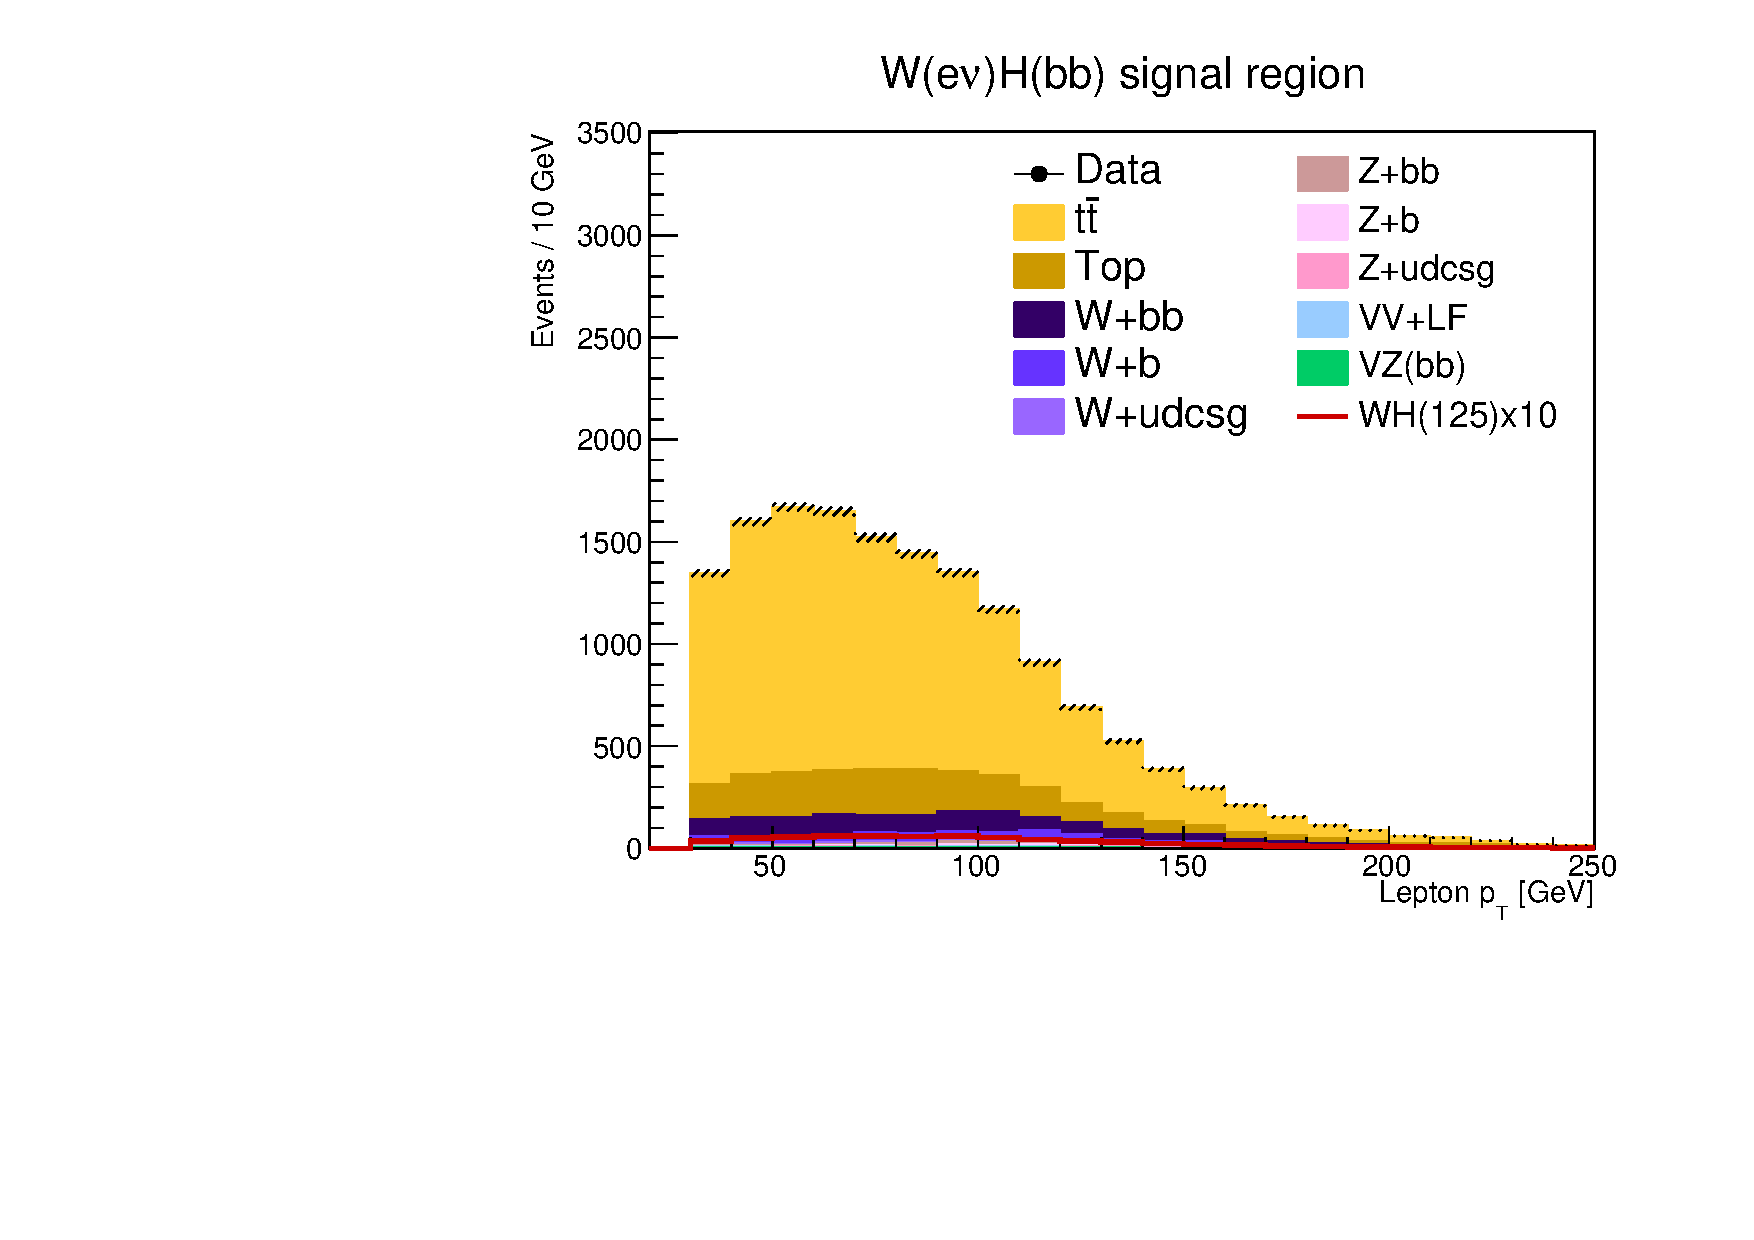
\includegraphics[width=0.48\textwidth]{figures/wlnhbb2016/resolved/WenWHSR_lepton1Pt.pdf}
    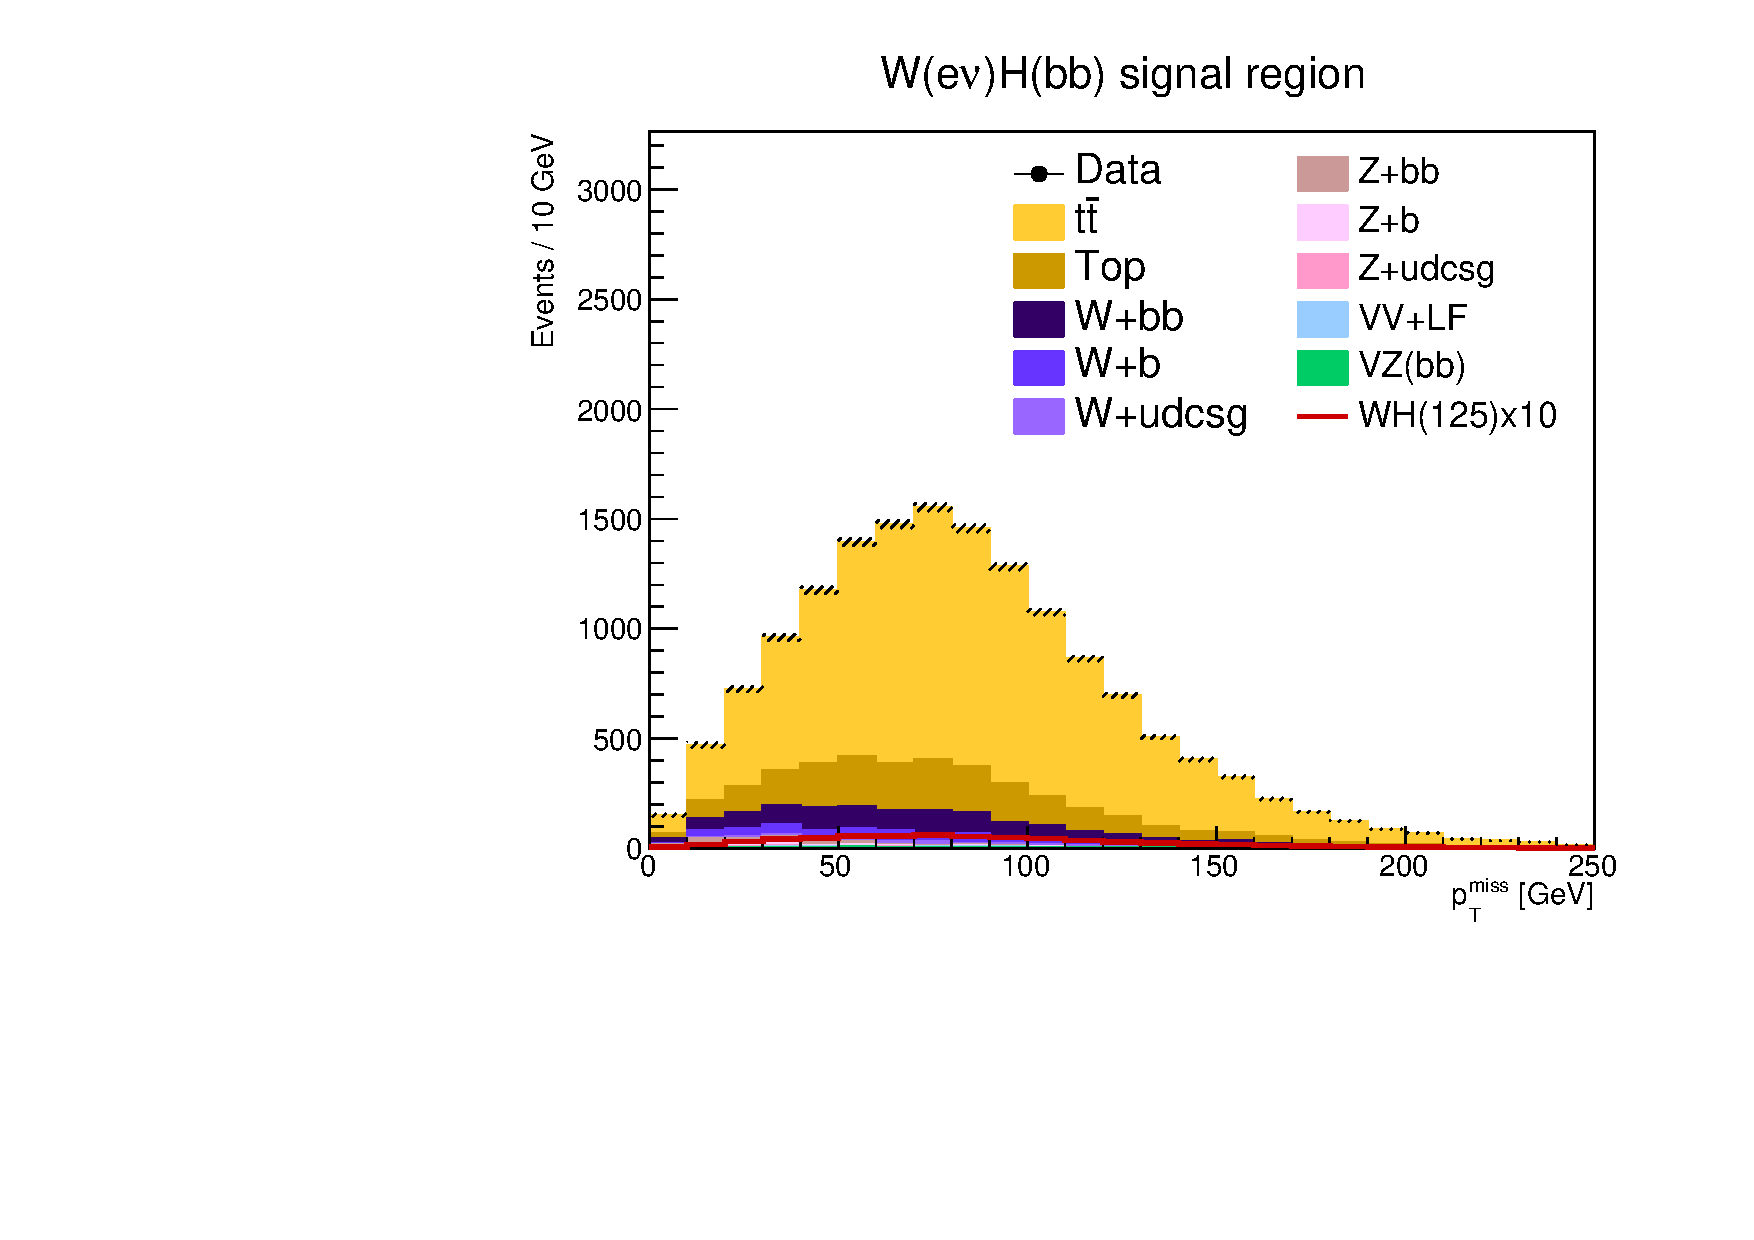
\includegraphics[width=0.48\textwidth]{figures/wlnhbb2016/resolved/WenWHSR_pfmet.pdf}
    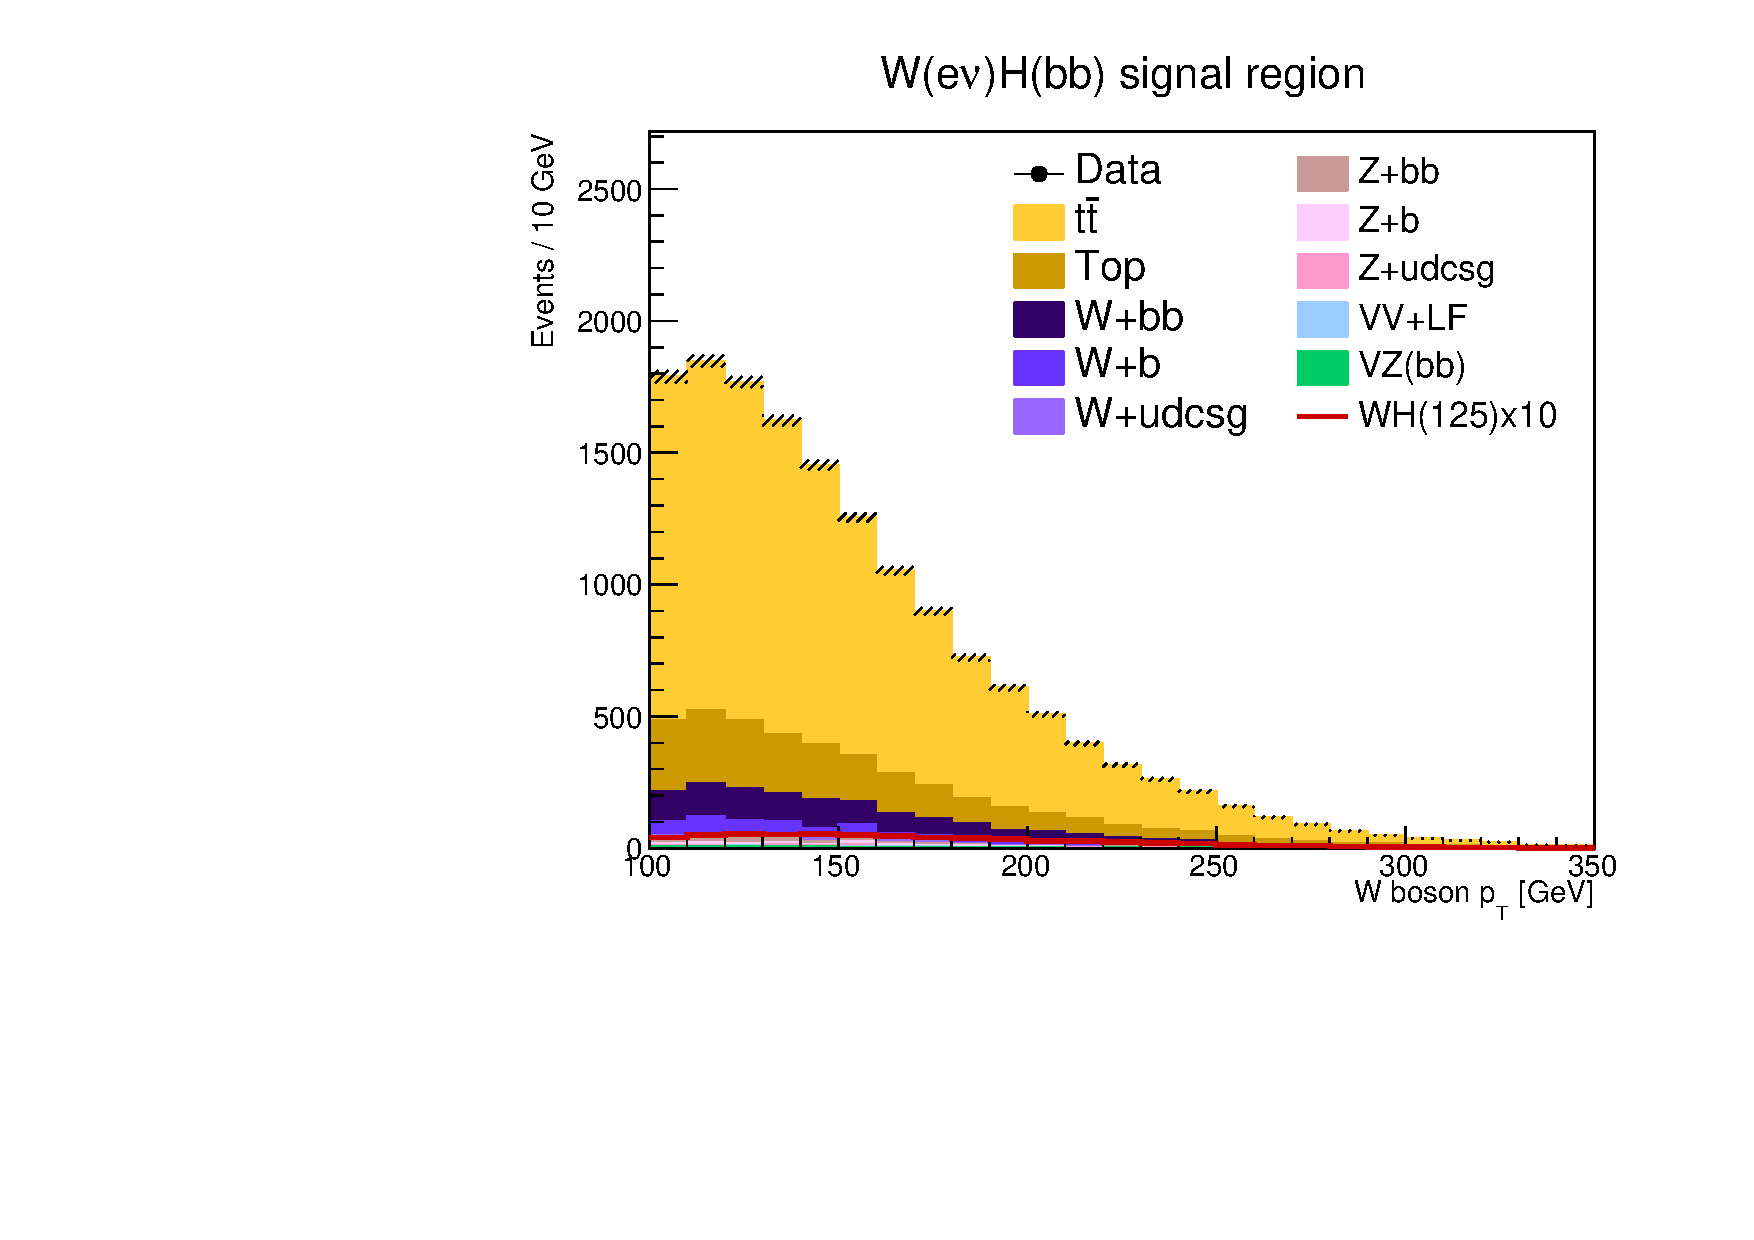
\includegraphics[width=0.48\textwidth]{figures/wlnhbb2016/resolved/WenWHSR_WpT.pdf}
    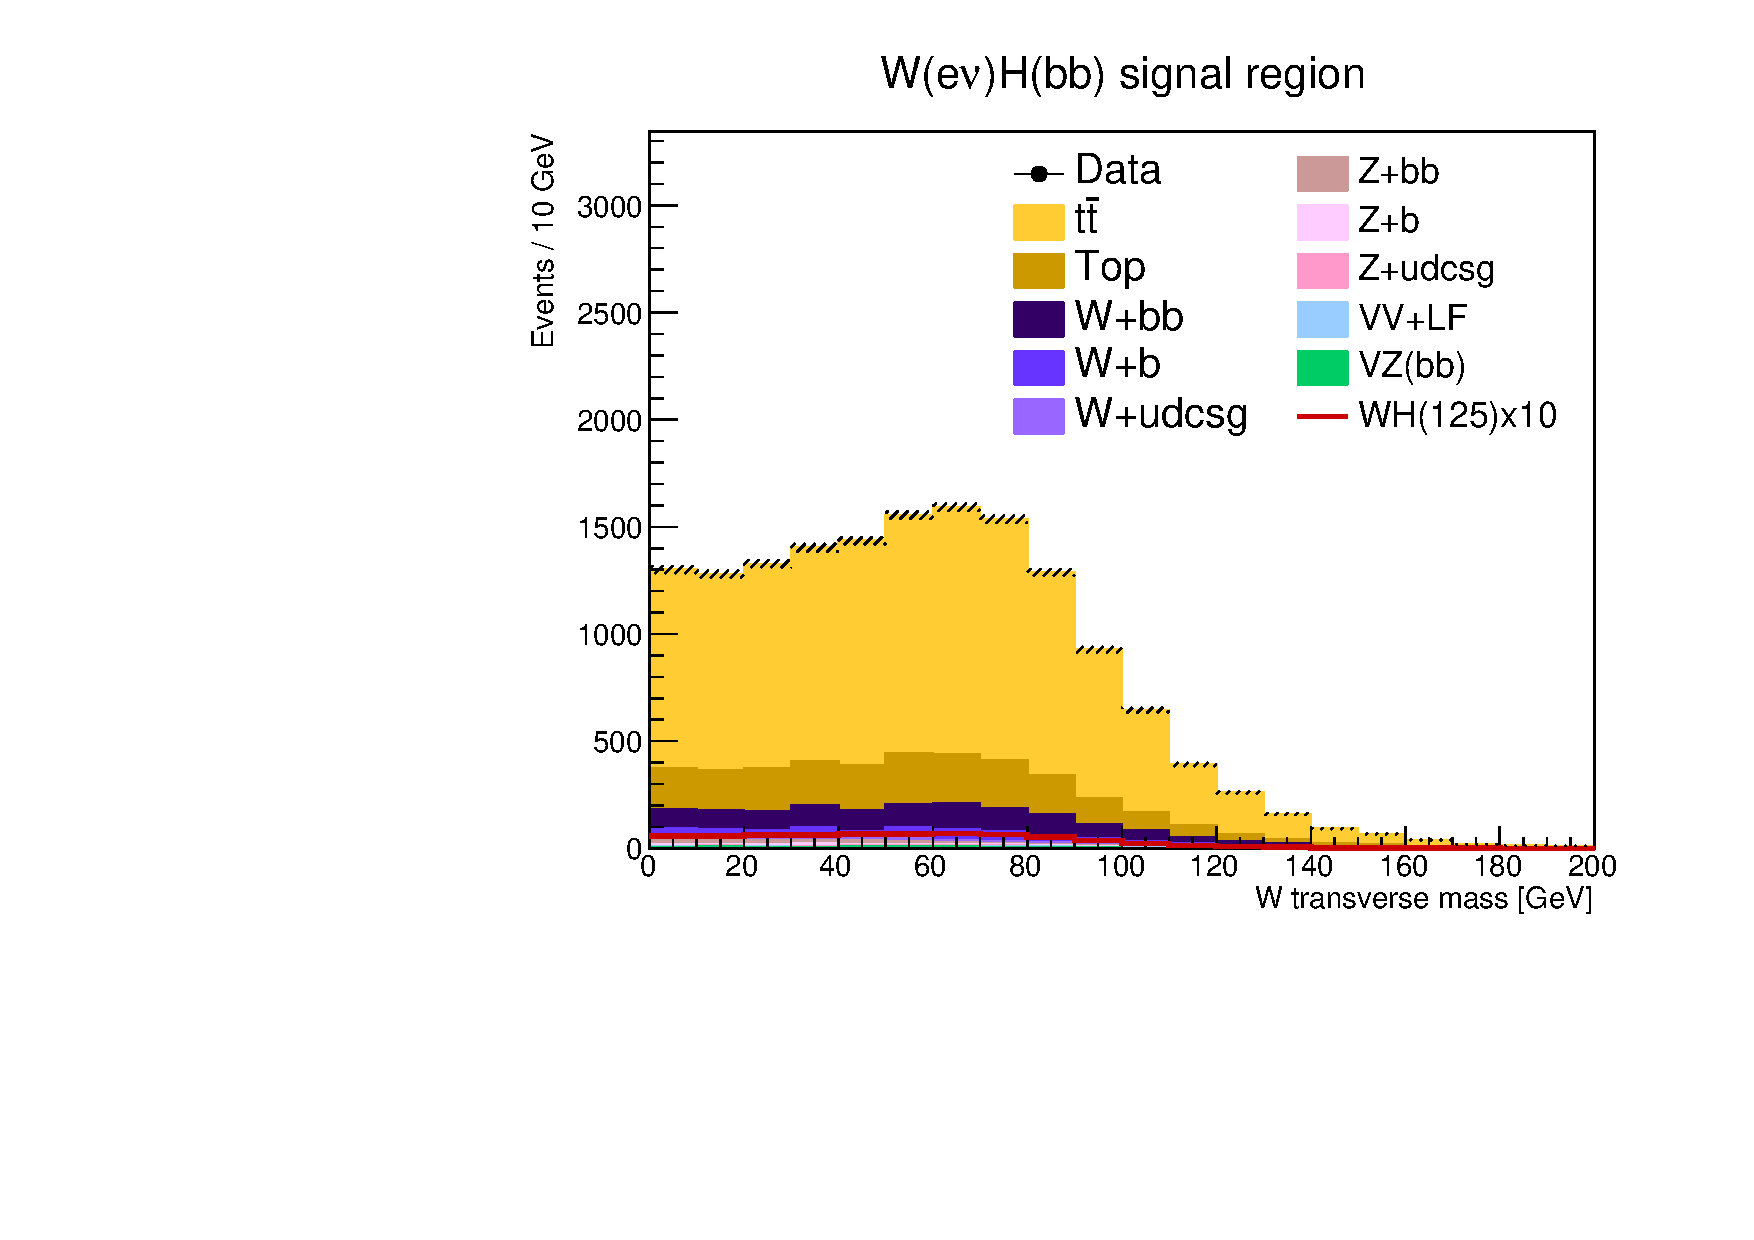
\includegraphics[width=0.48\textwidth]{figures/wlnhbb2016/resolved/WenWHSR_mTW.pdf}
    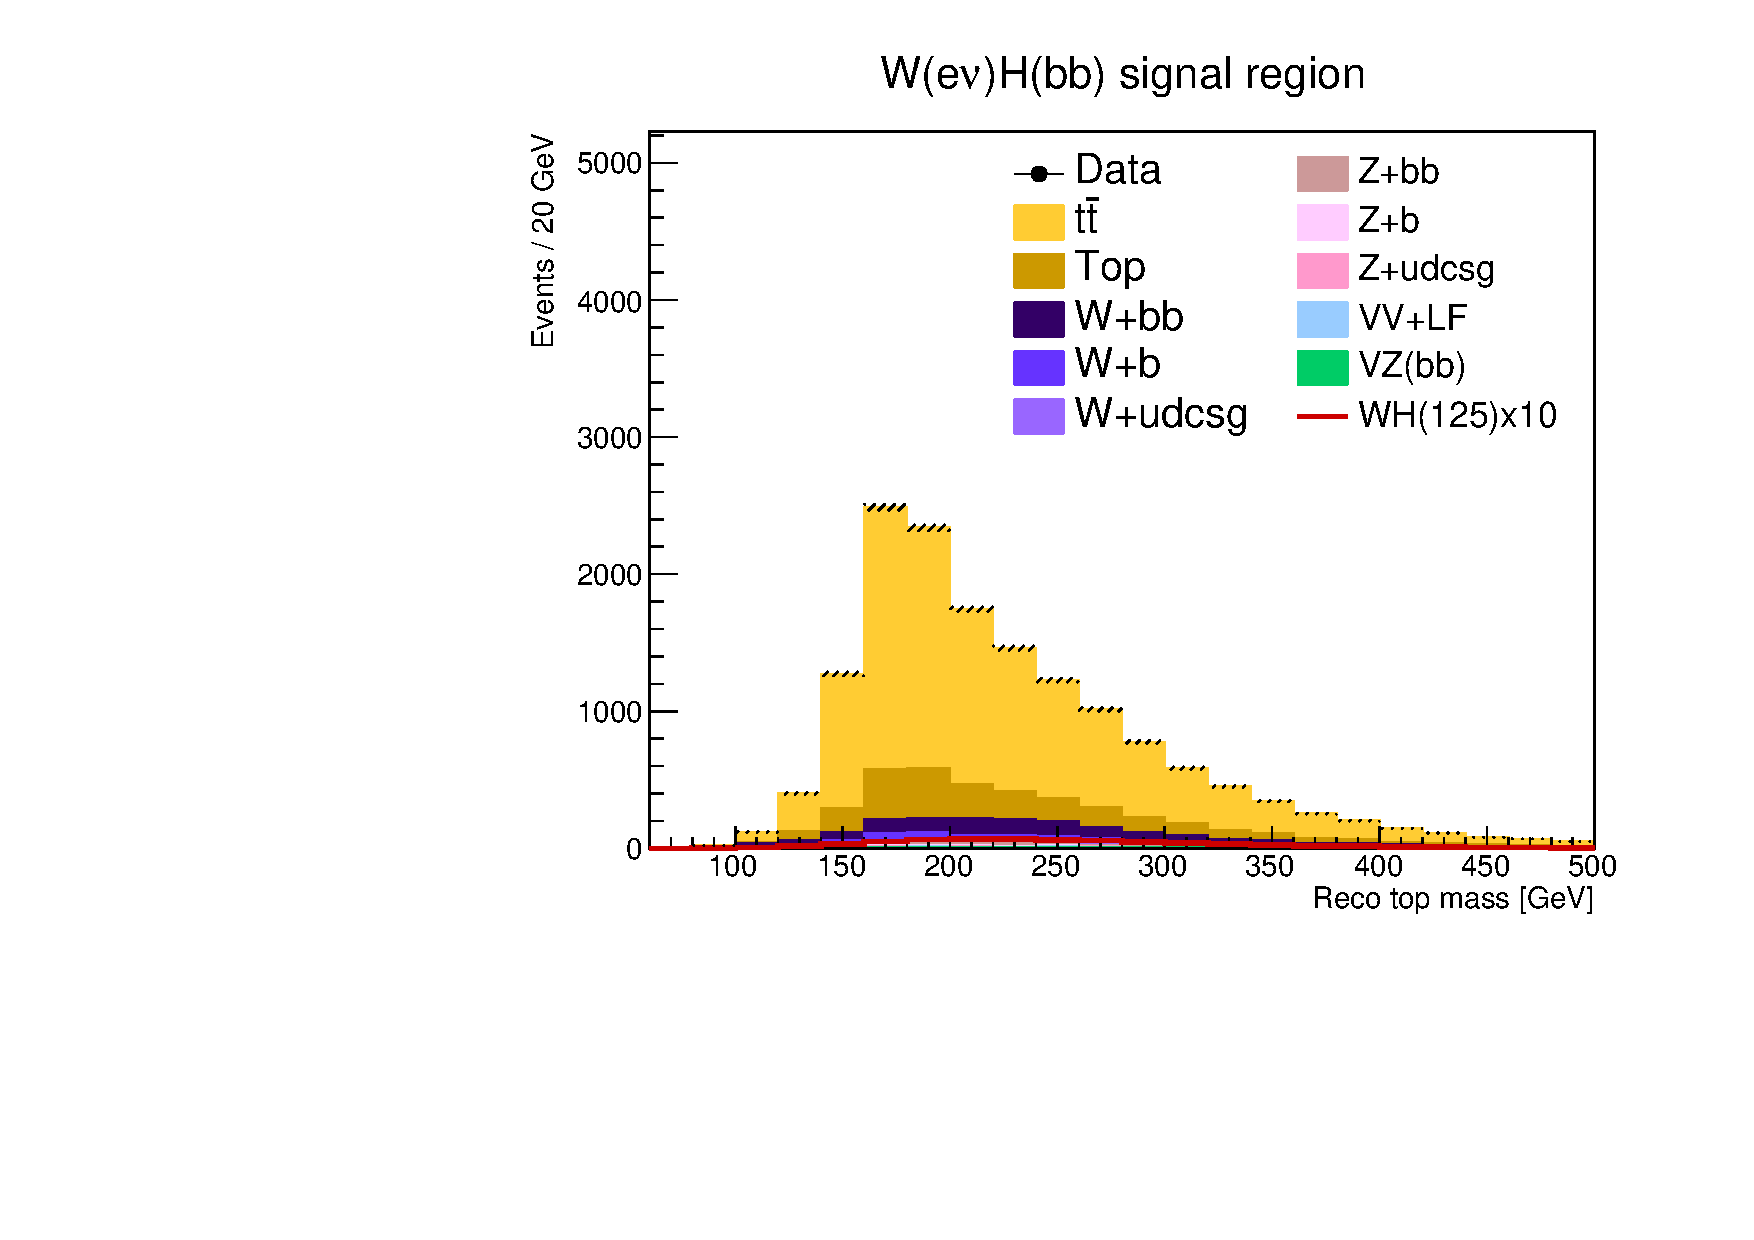
\includegraphics[width=0.48\textwidth]{figures/wlnhbb2016/resolved/WenWHSR_topMassLep1Met.pdf}
    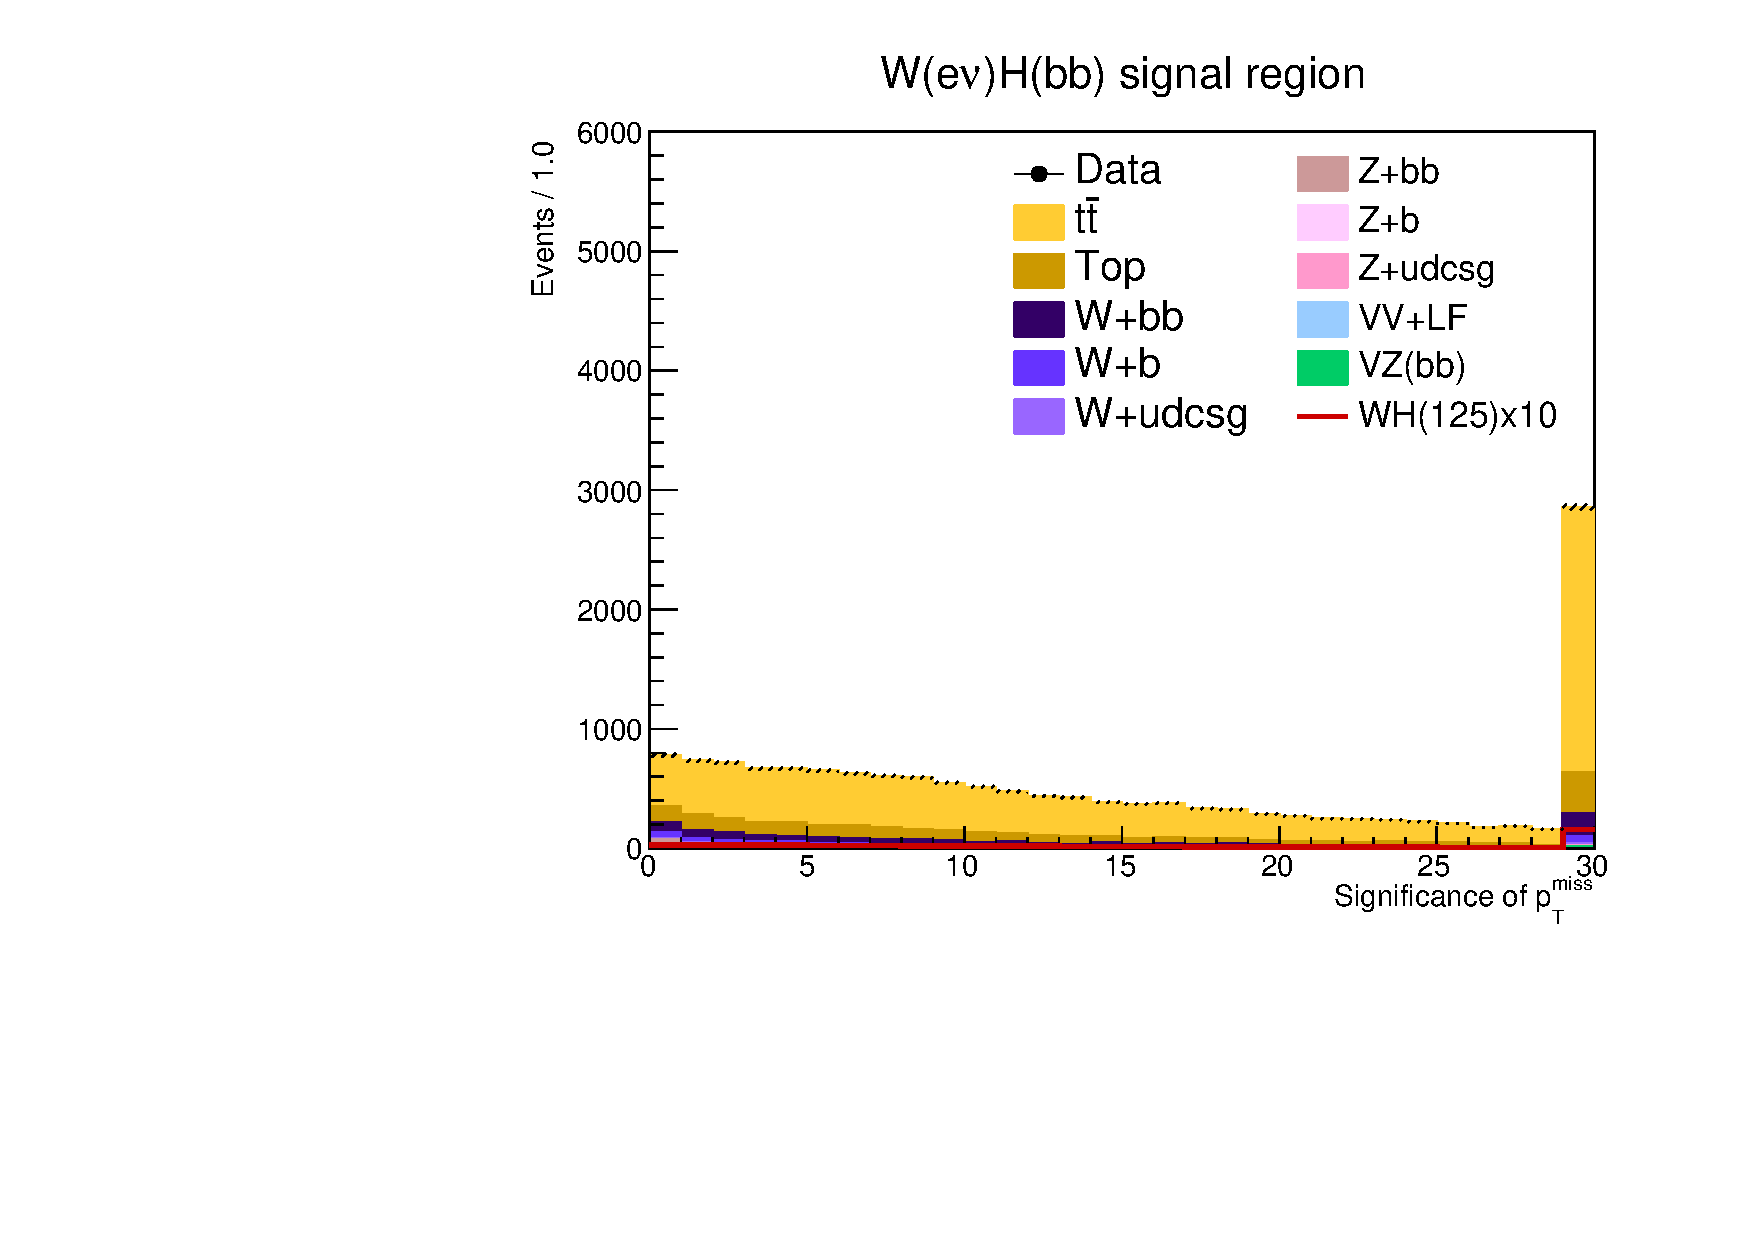
\includegraphics[width=0.48\textwidth]{figures/wlnhbb2016/resolved/WenWHSR_pfmetsig.pdf}
    \caption{W boson reconstruction in the resolved category W(e$\nu$) signal region.
    Left to right and top to bottom: electron $\pt$, $\MET$, W boson $\pt$, W boson transverse mass,
    the reconstructed top quark mass, and the $\MET$ significance.
    The simulated shapes are prefit, with the postfit normalizations applied.}
    \label{fig:res_WenSR_WBosons}
  \end{center}
\end{figure}
\clearpage

\begin{figure}[tbp]
  \begin{center}
    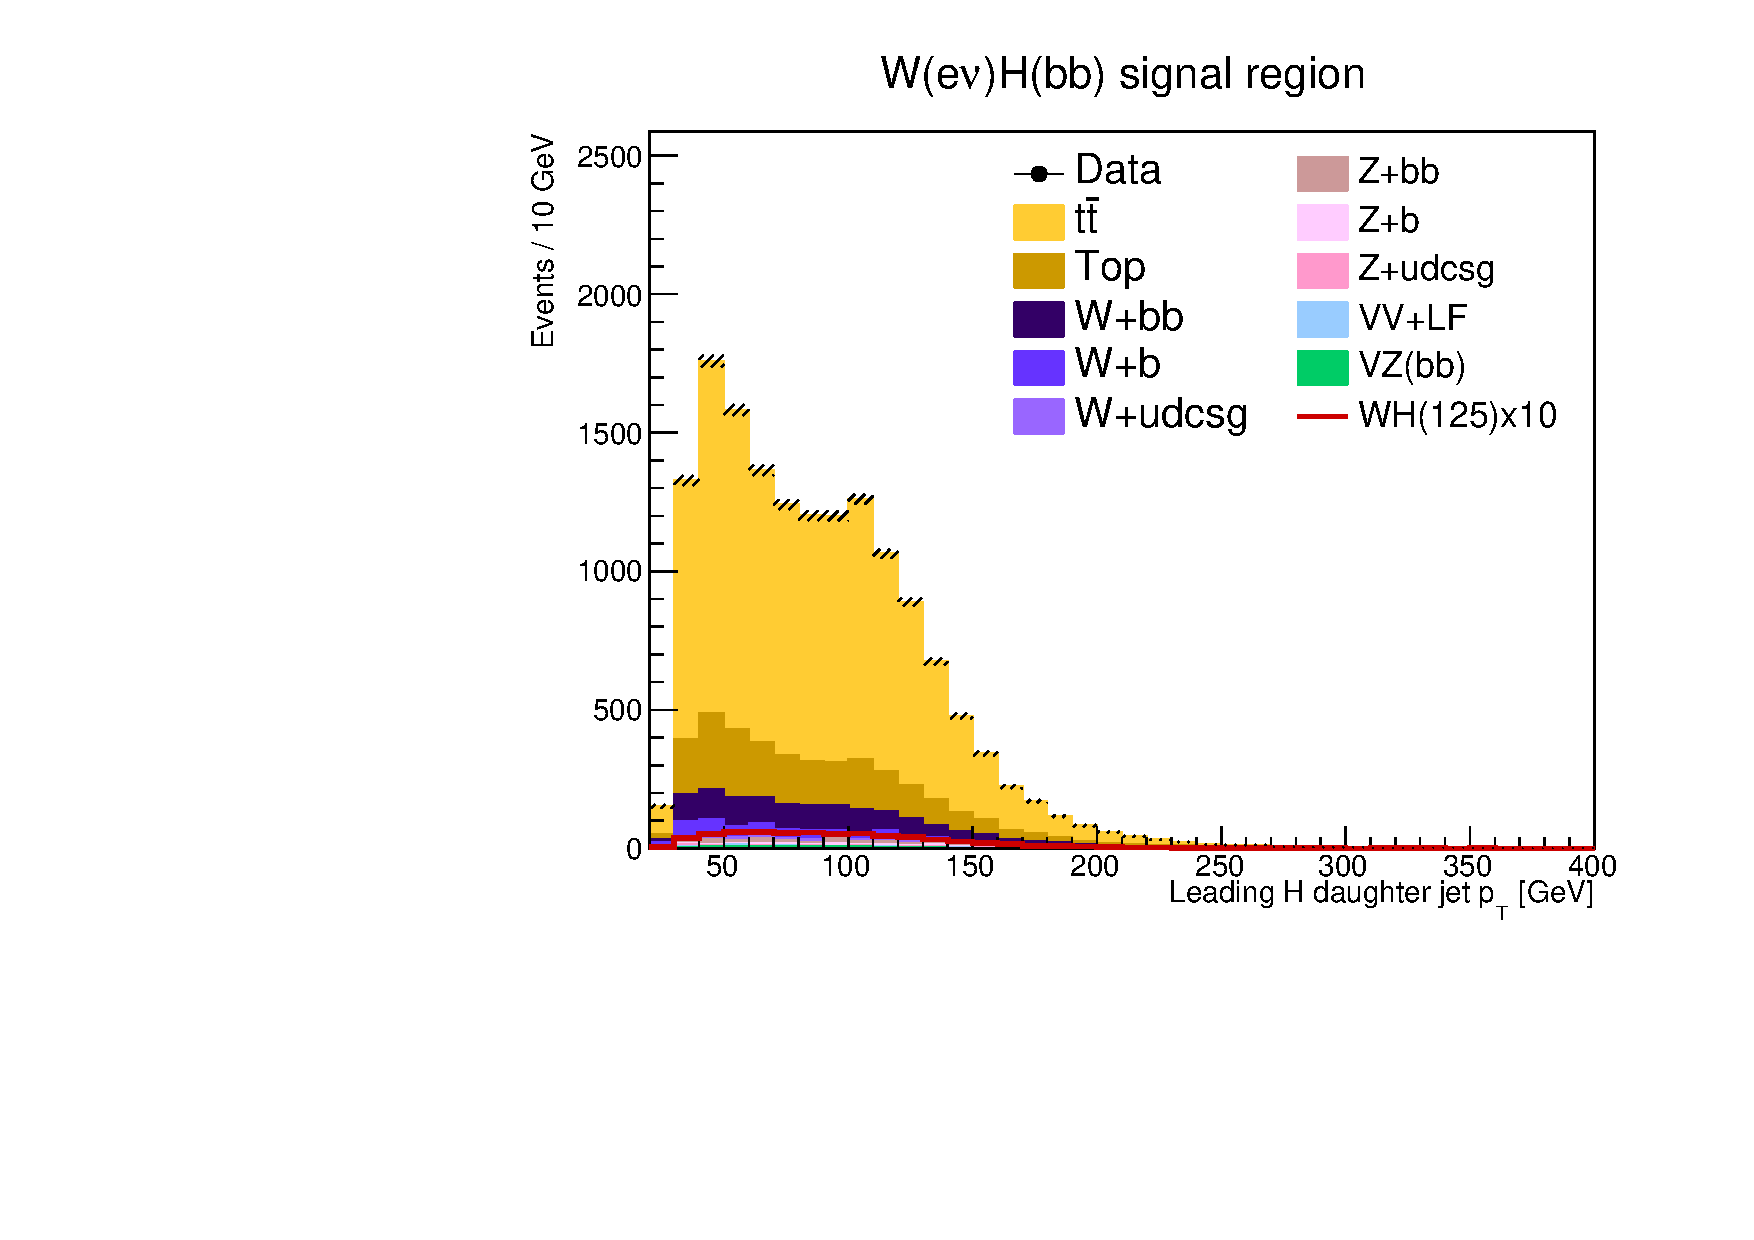
\includegraphics[width=0.48\textwidth]{figures/wlnhbb2016/resolved/WenWHSR_Hbjet1Pt.pdf}
    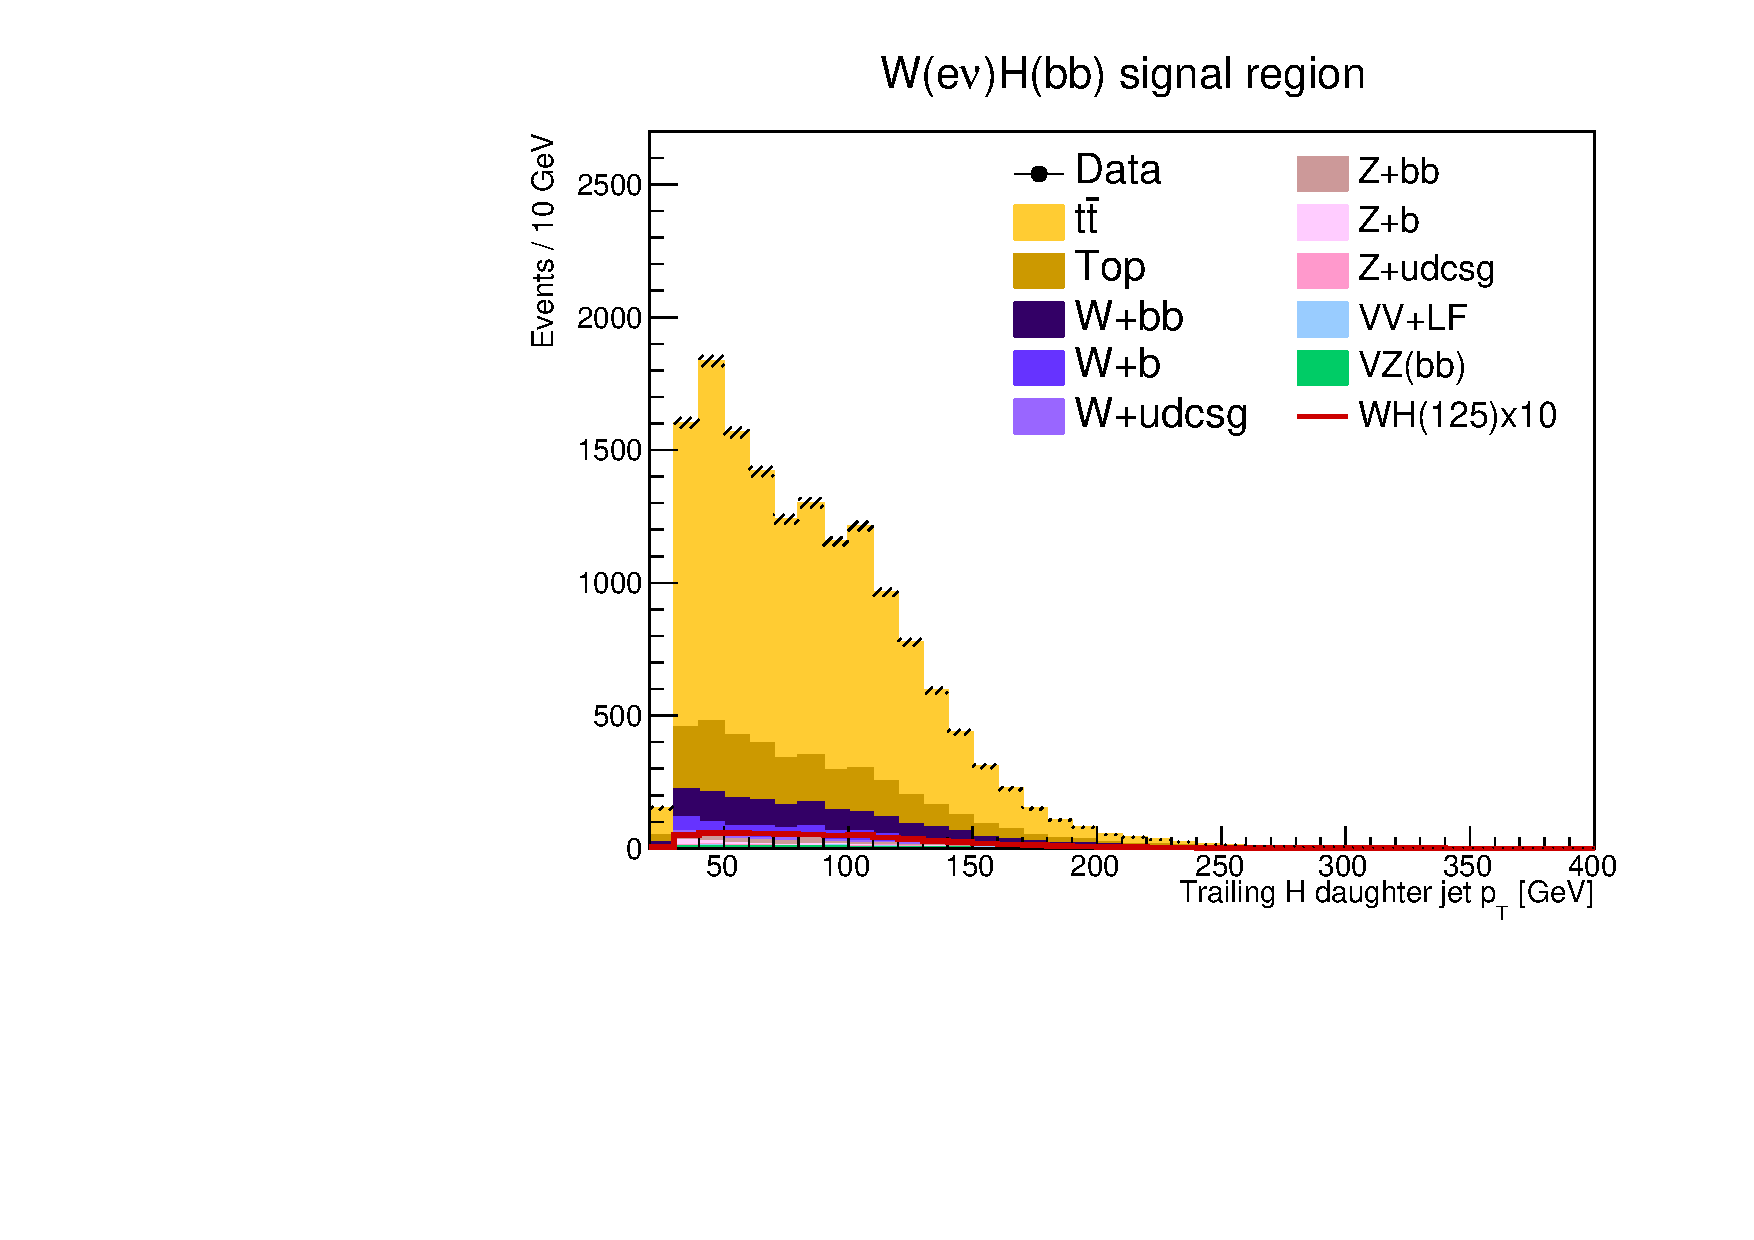
\includegraphics[width=0.48\textwidth]{figures/wlnhbb2016/resolved/WenWHSR_Hbjet2Pt.pdf}
    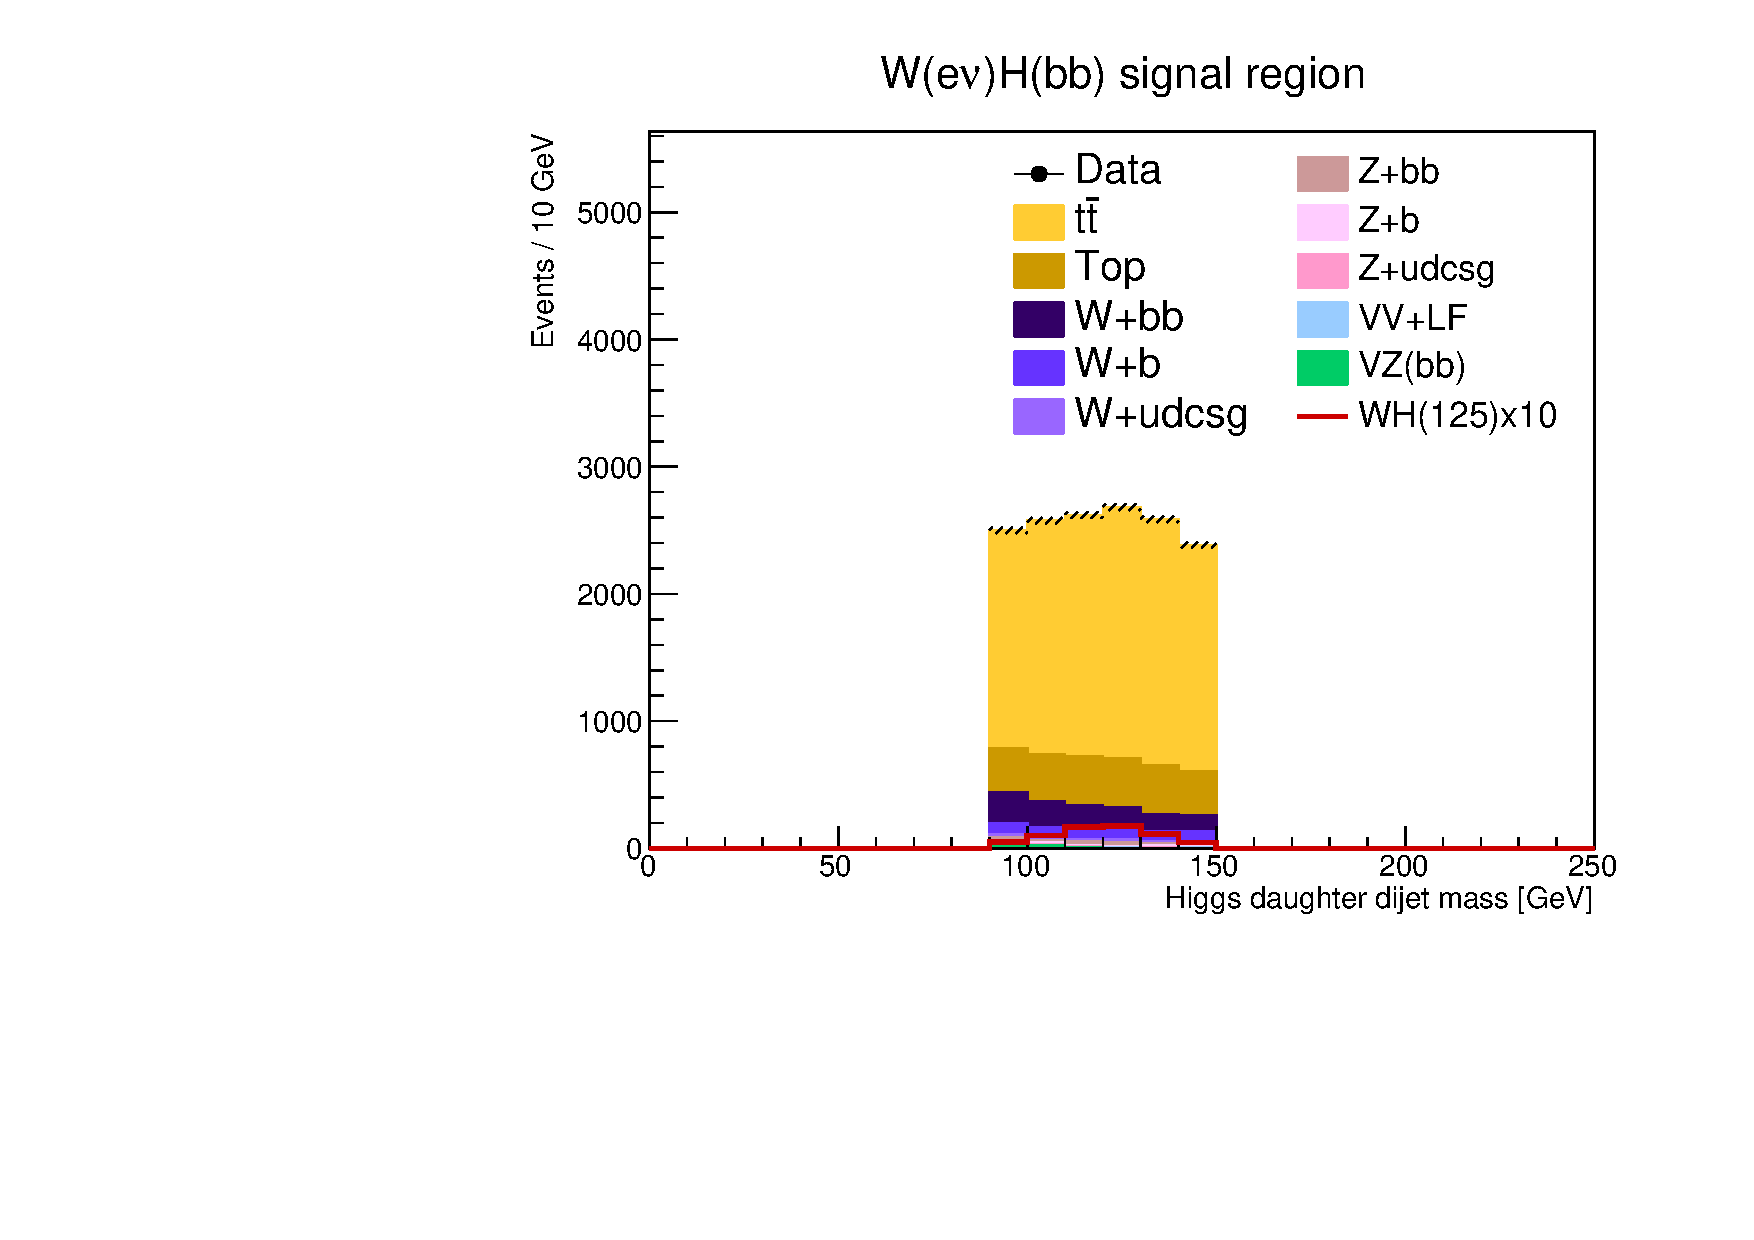
\includegraphics[width=0.48\textwidth]{figures/wlnhbb2016/resolved/WenWHSR_mH.pdf}
    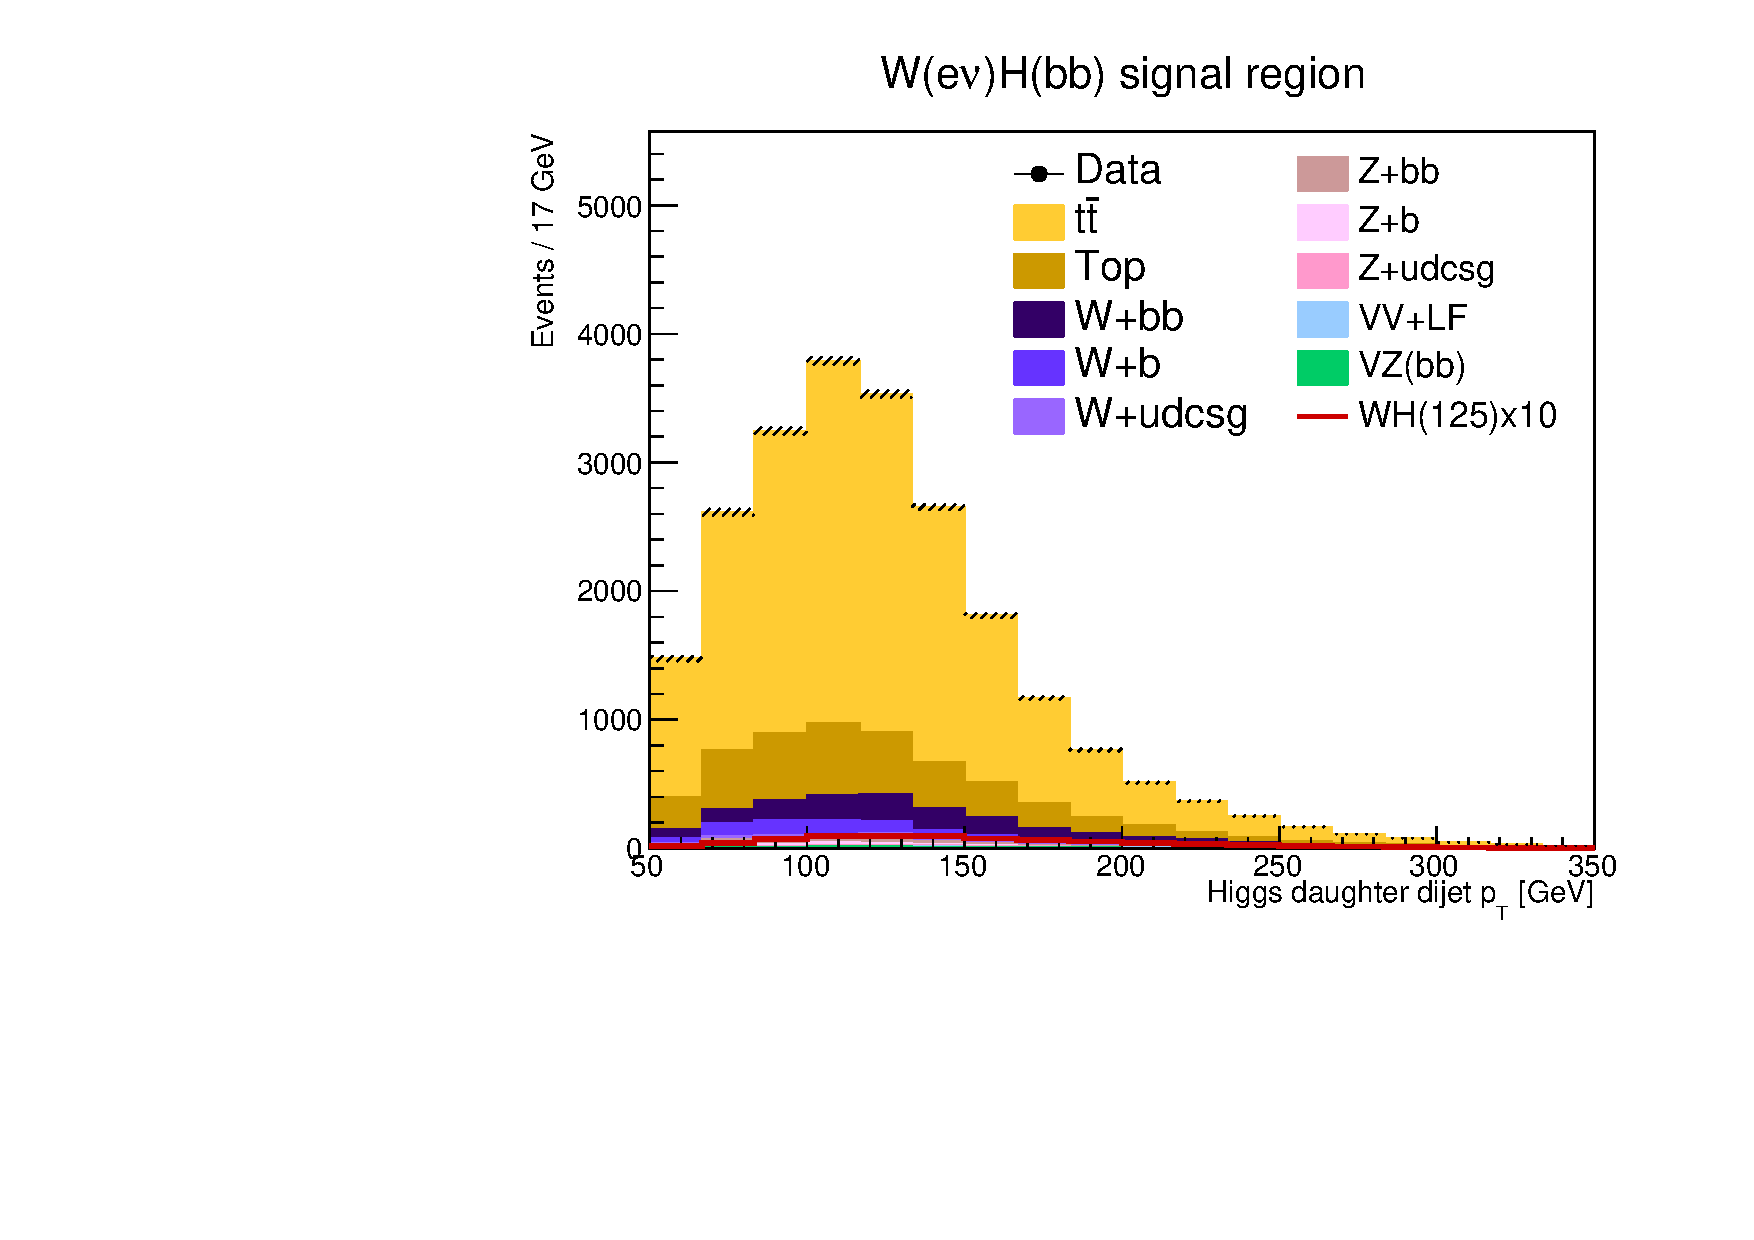
\includegraphics[width=0.48\textwidth]{figures/wlnhbb2016/resolved/WenWHSR_pTH.pdf}
    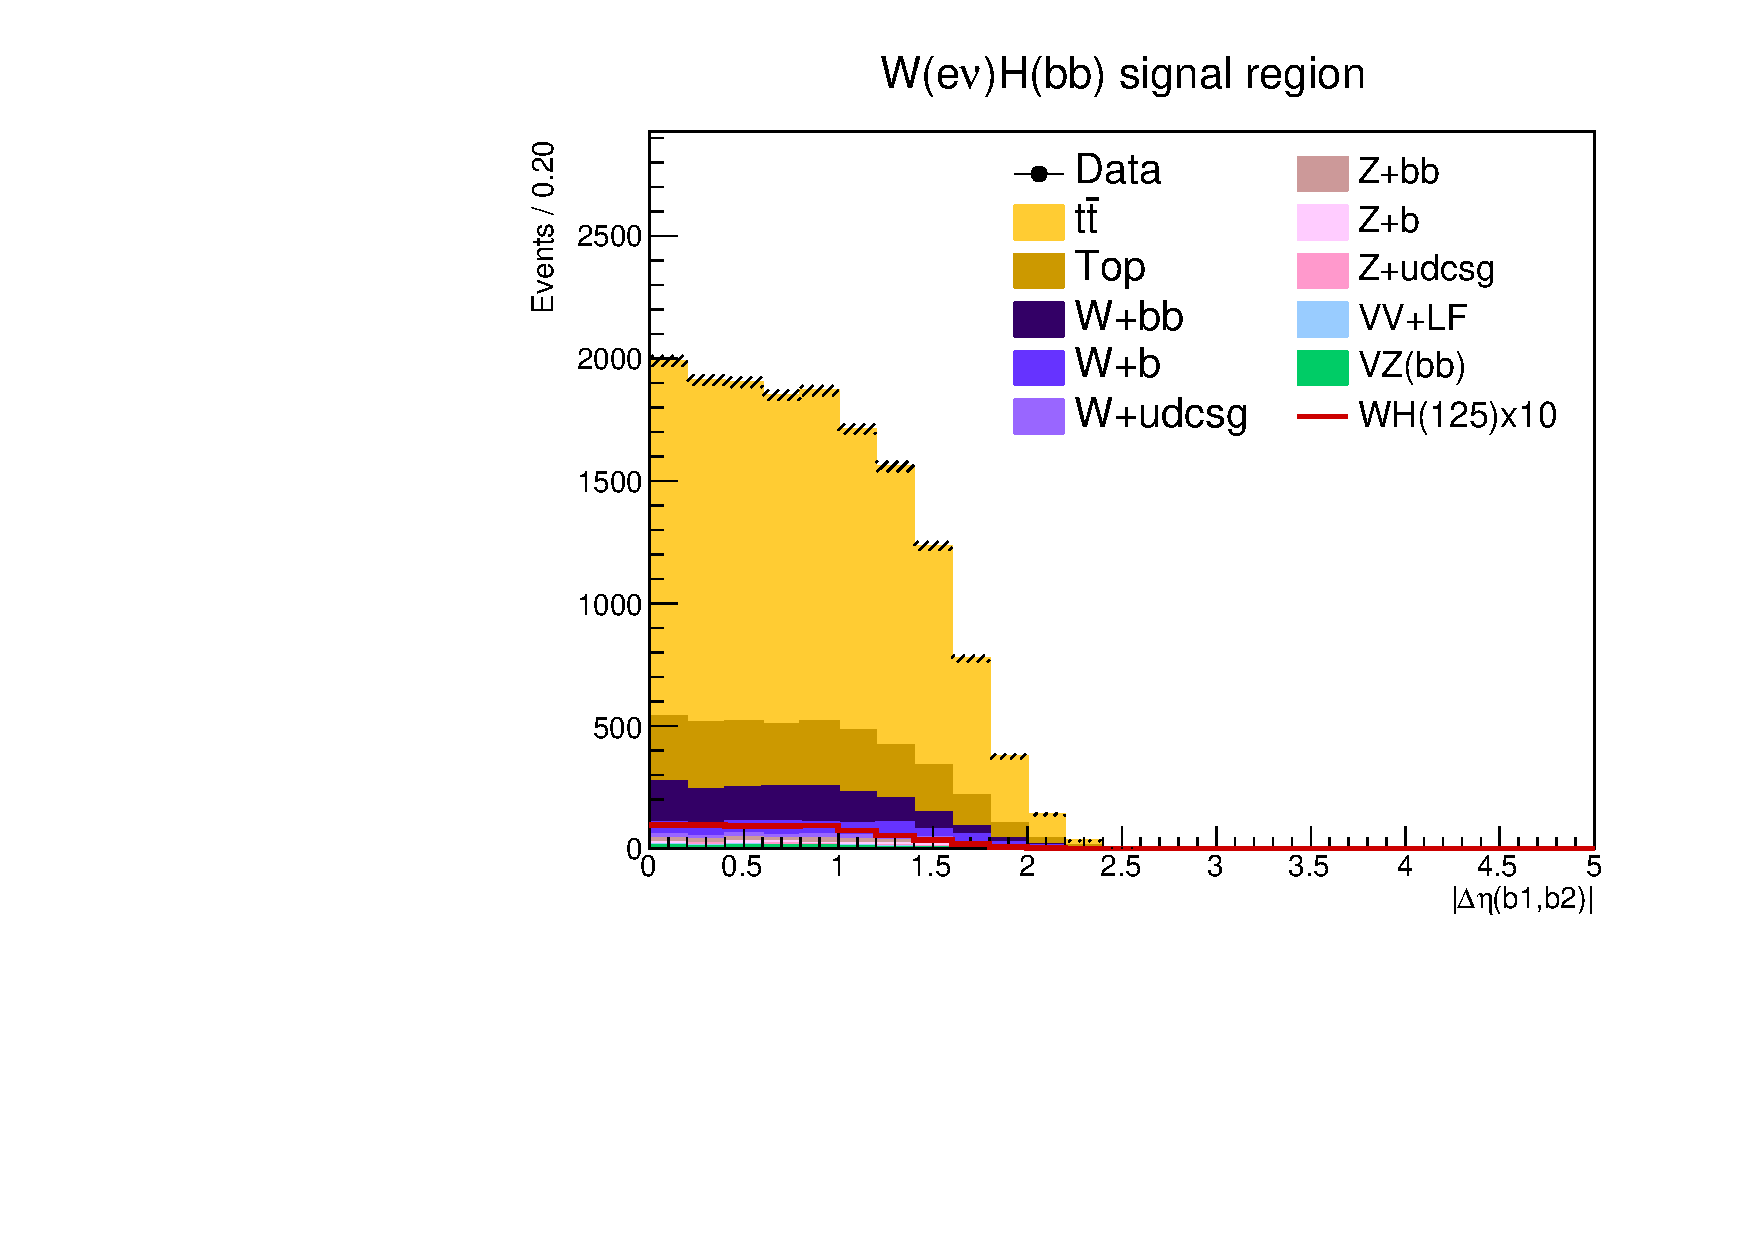
\includegraphics[width=0.48\textwidth]{figures/wlnhbb2016/resolved/WenWHSR_dEtab1b2.pdf}
    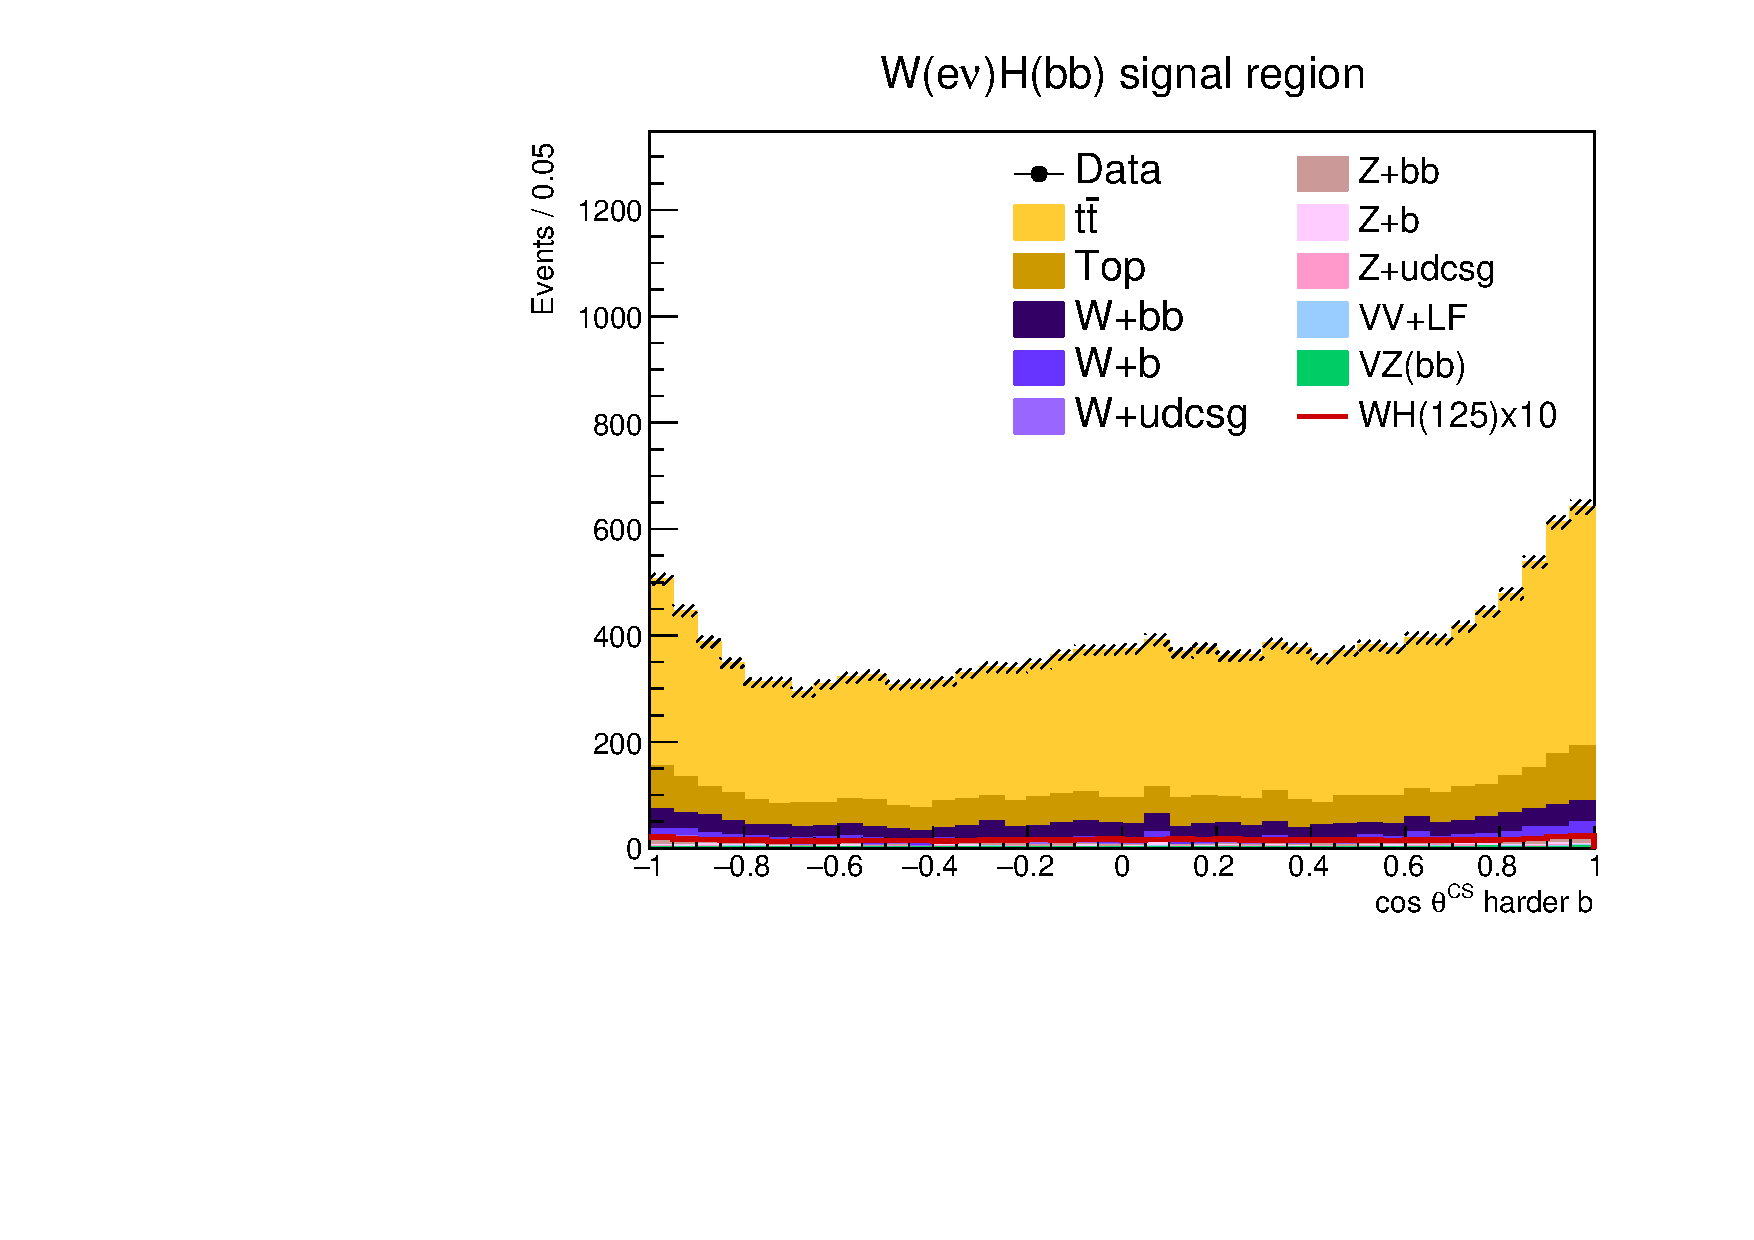
\includegraphics[width=0.48\textwidth]{figures/wlnhbb2016/resolved/WenWHSR_hbbCosThetaCSJ1.pdf}
    \caption{\HBB\ reconstruction in the resolved category W(e$\nu$) signal region.
    Left to right and top to bottom: higher b-tagged jet $\pt$, lower b-tagged jet $\pt$, dijet mass, dijet $\pt$, 
    pseudorapidity difference between the two jets, and the Collins-Soper angle of the harder b-tagged jet.
    The simulated shapes are prefit, with the postfit normalizations applied.}
    \label{fig:res_WenSR_Hbb}
  \end{center}
\end{figure}
\clearpage

\begin{figure}[tbp]
  \begin{center}
    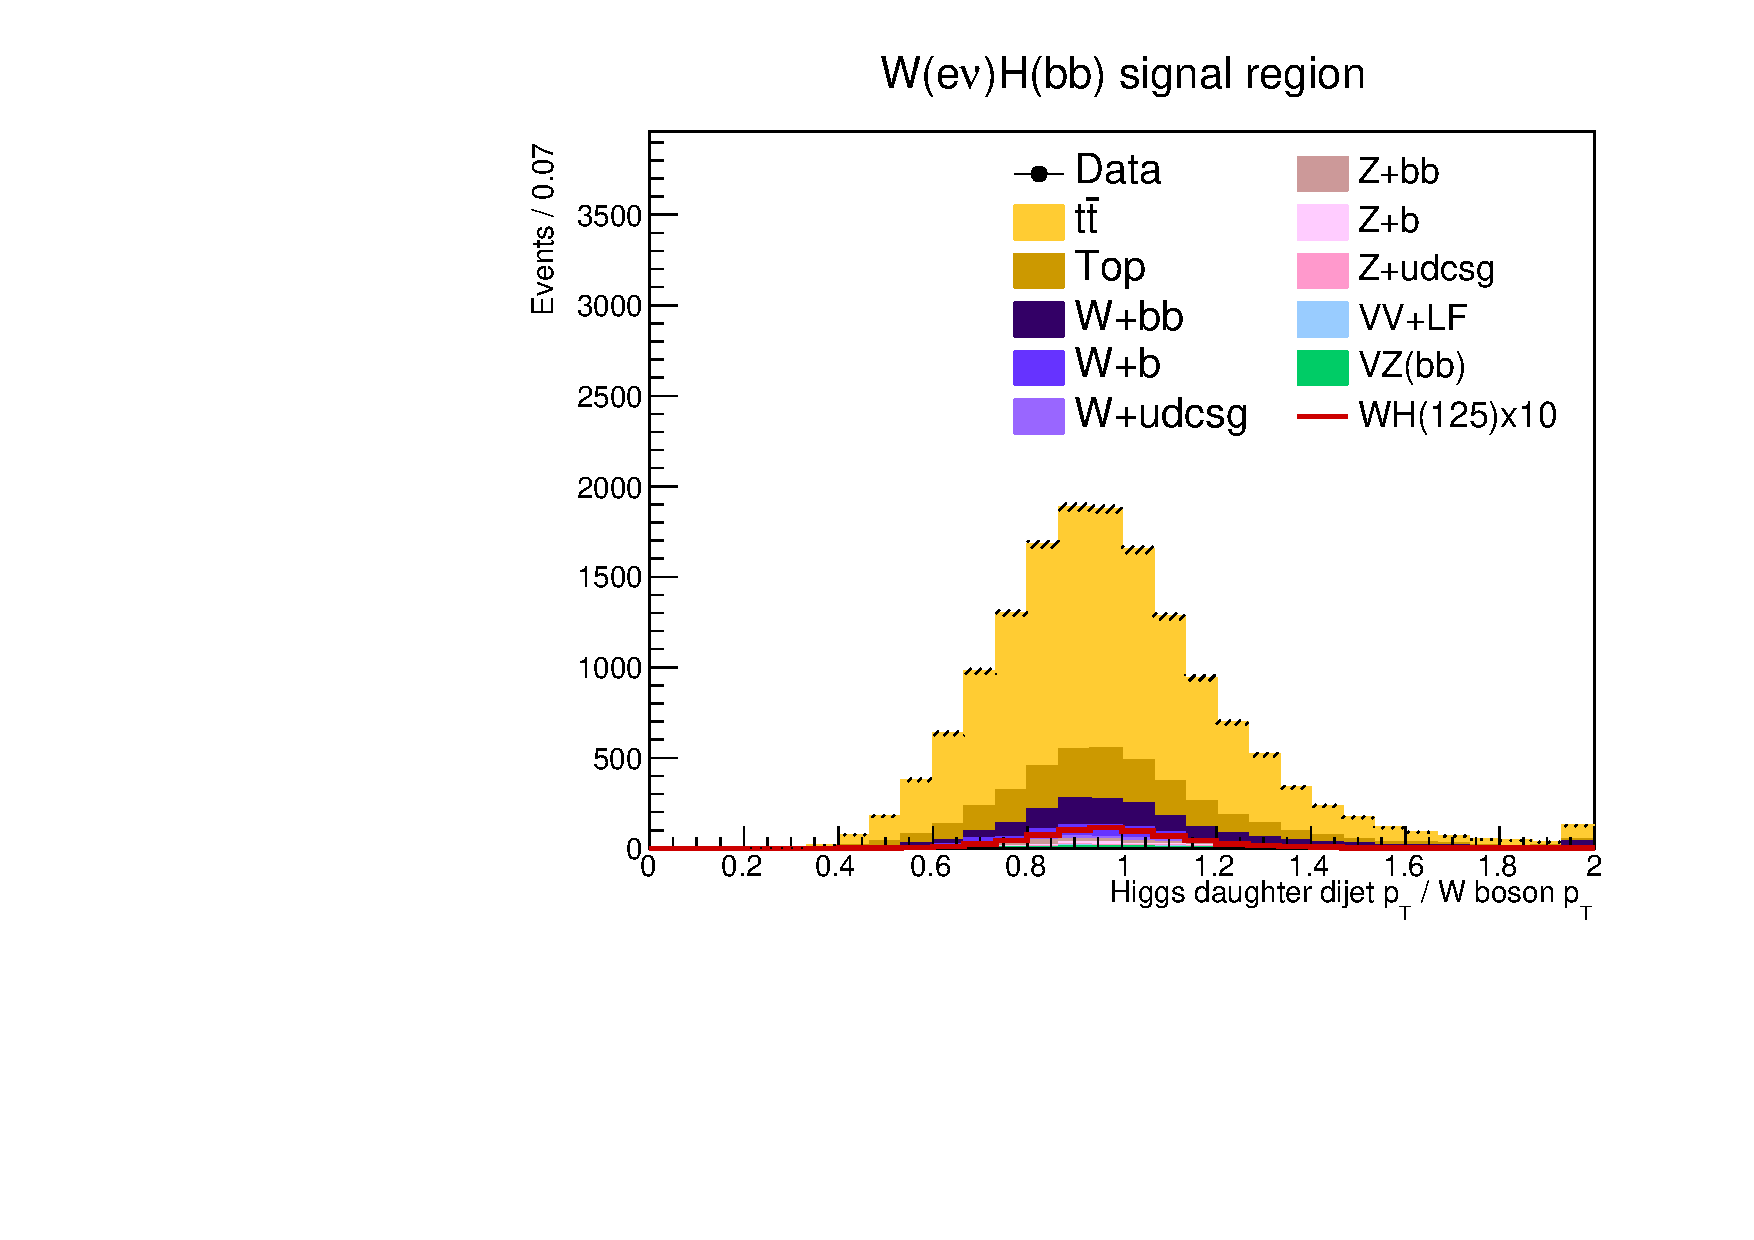
\includegraphics[width=0.48\textwidth]{figures/wlnhbb2016/resolved/WenWHSR_pTBalanceDijetW.pdf}
    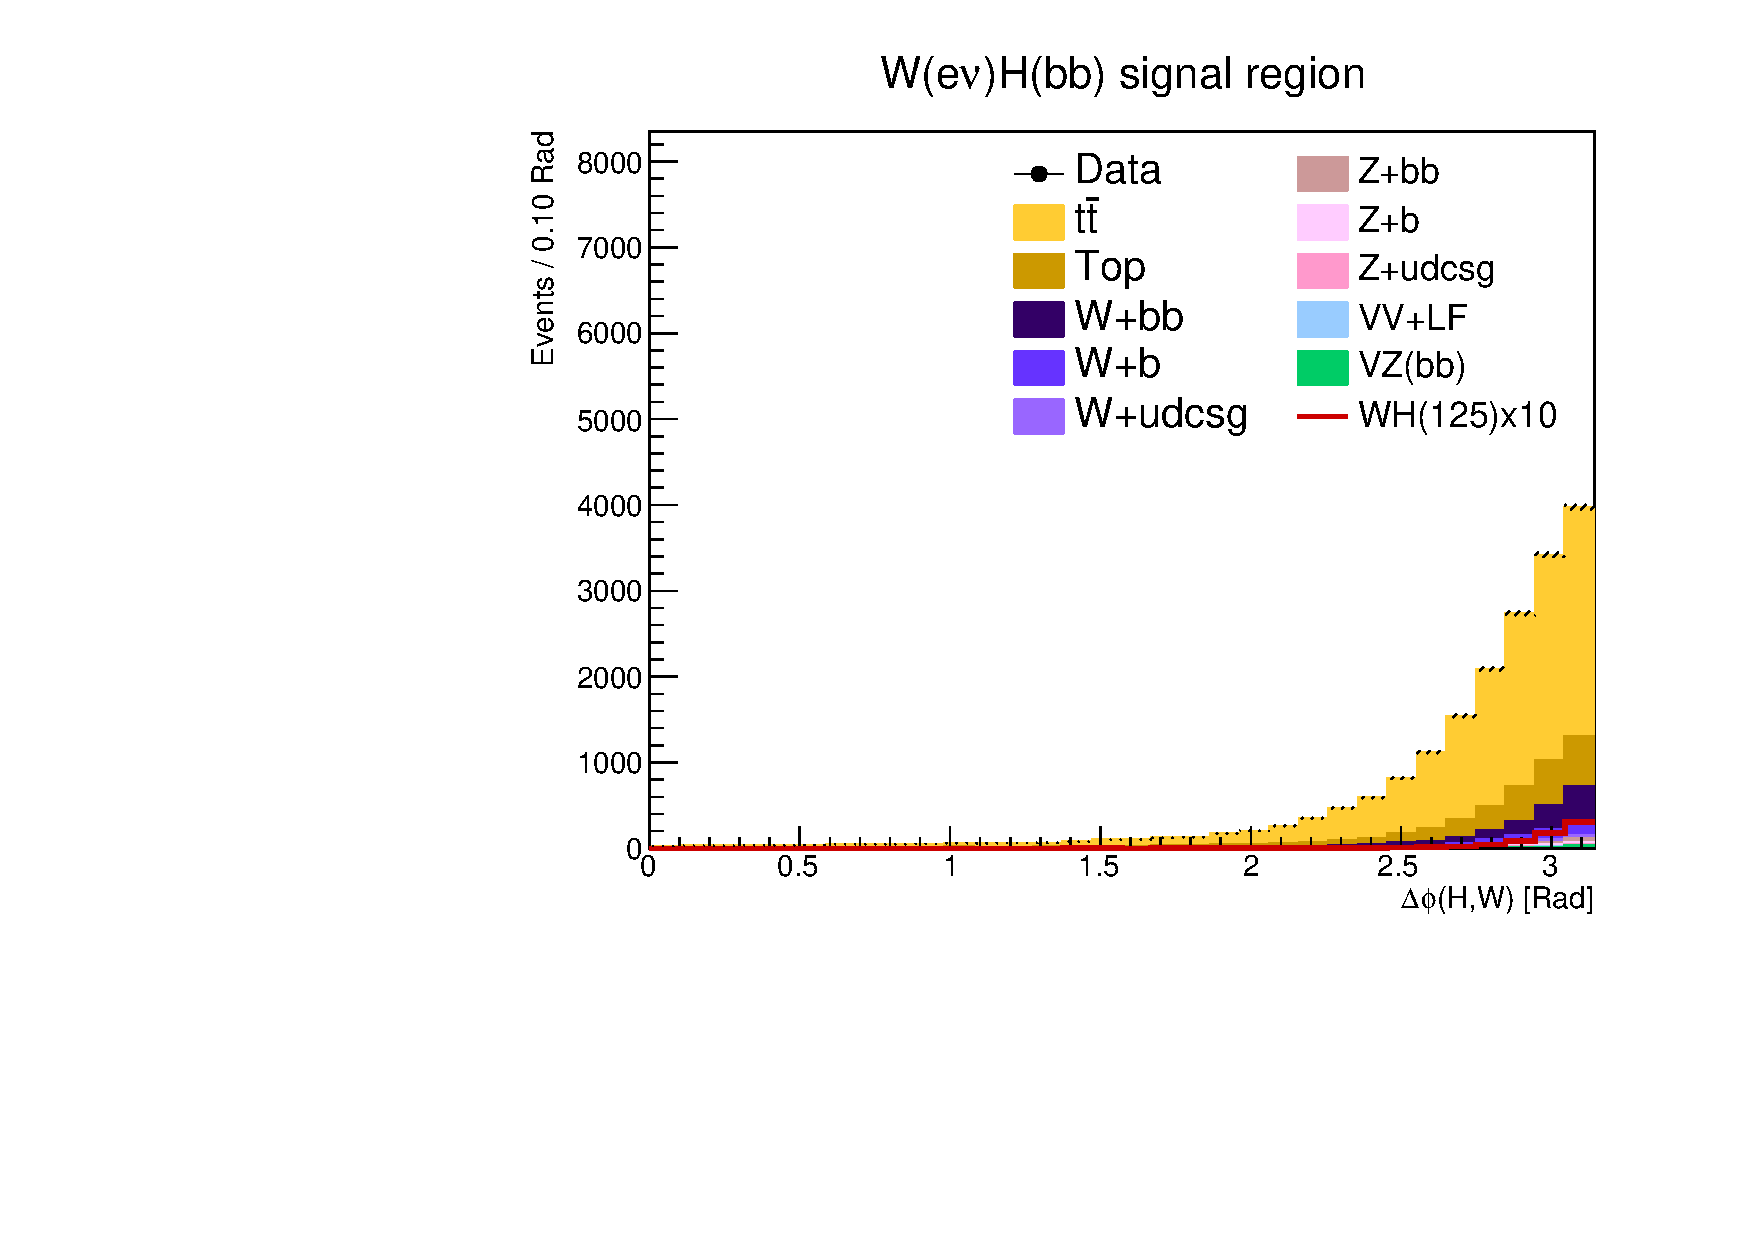
\includegraphics[width=0.48\textwidth]{figures/wlnhbb2016/resolved/WenWHSR_deltaPhiVH.pdf}
    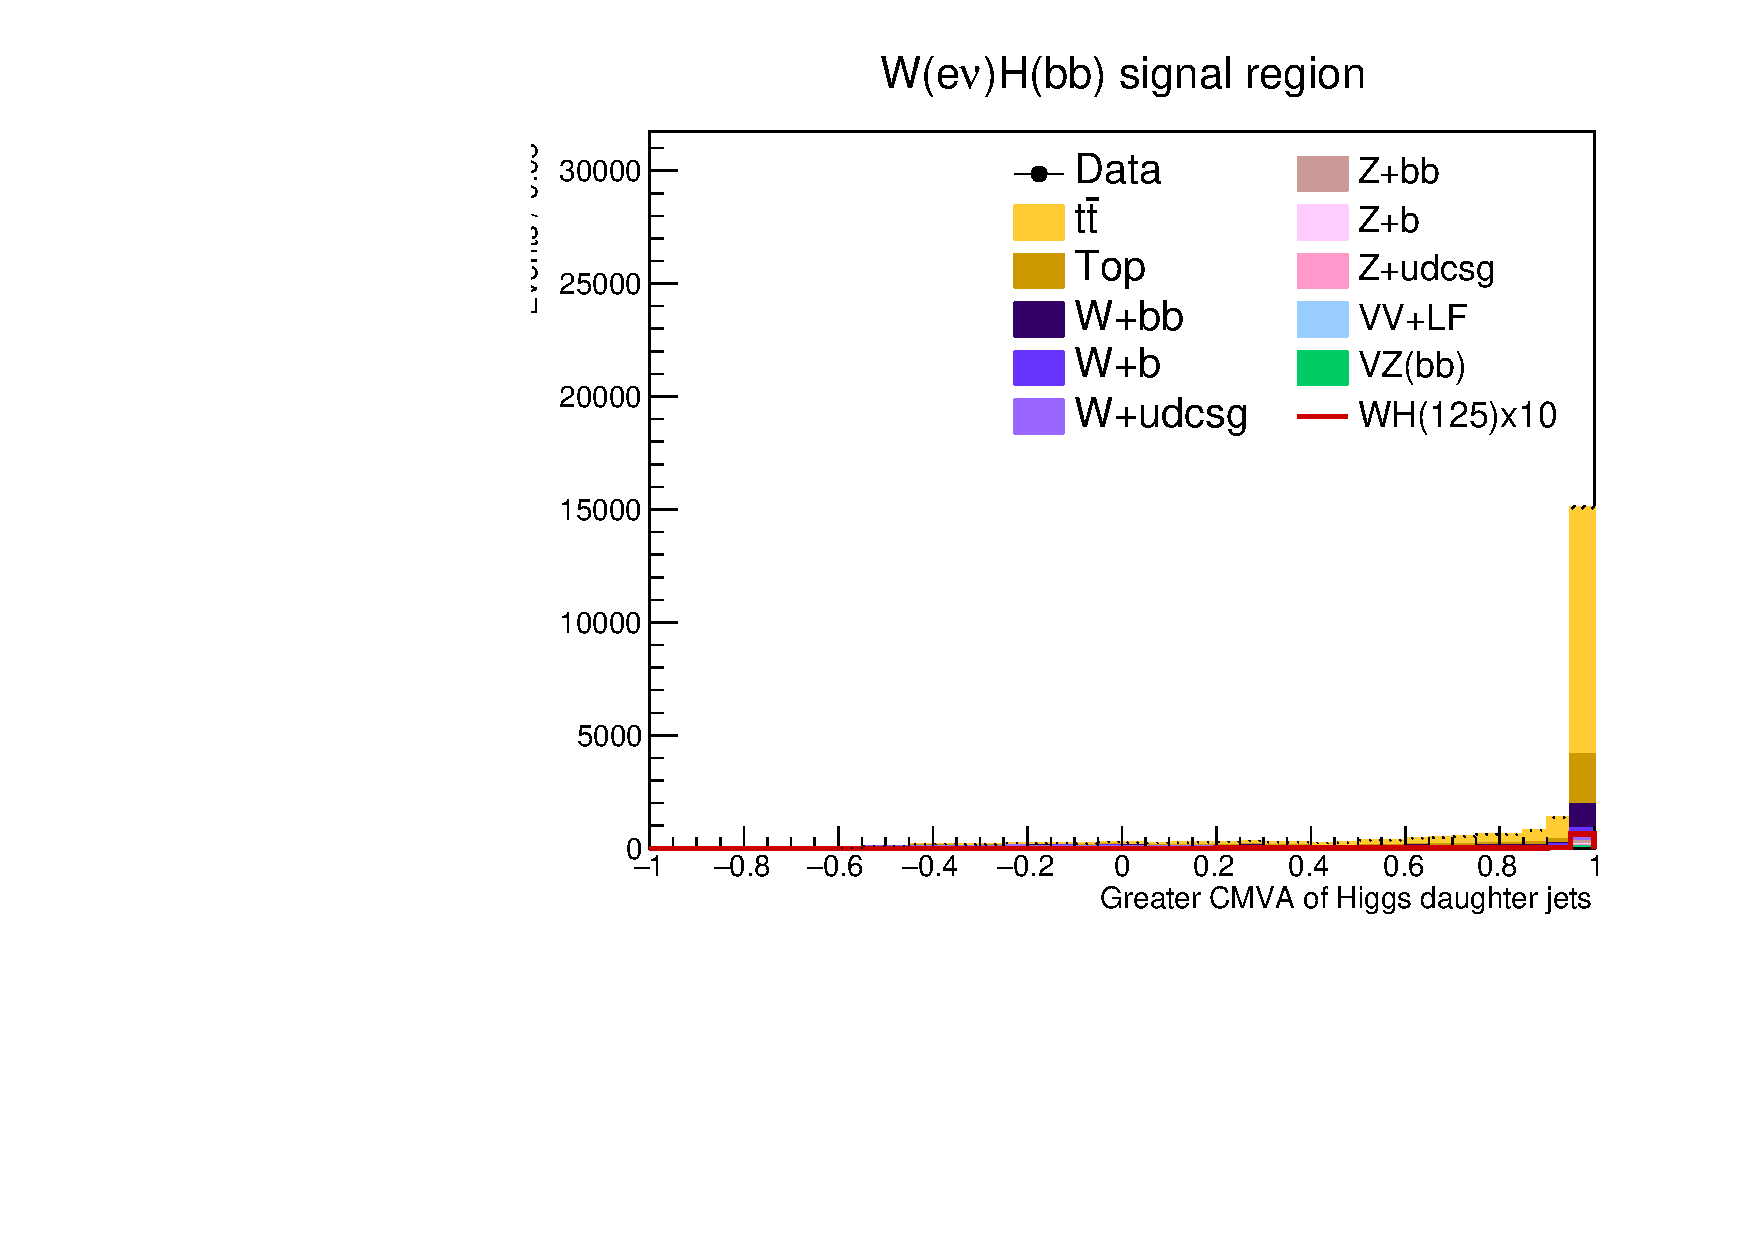
\includegraphics[width=0.48\textwidth]{figures/wlnhbb2016/resolved/WenWHSR_bDiscrMax.pdf}
    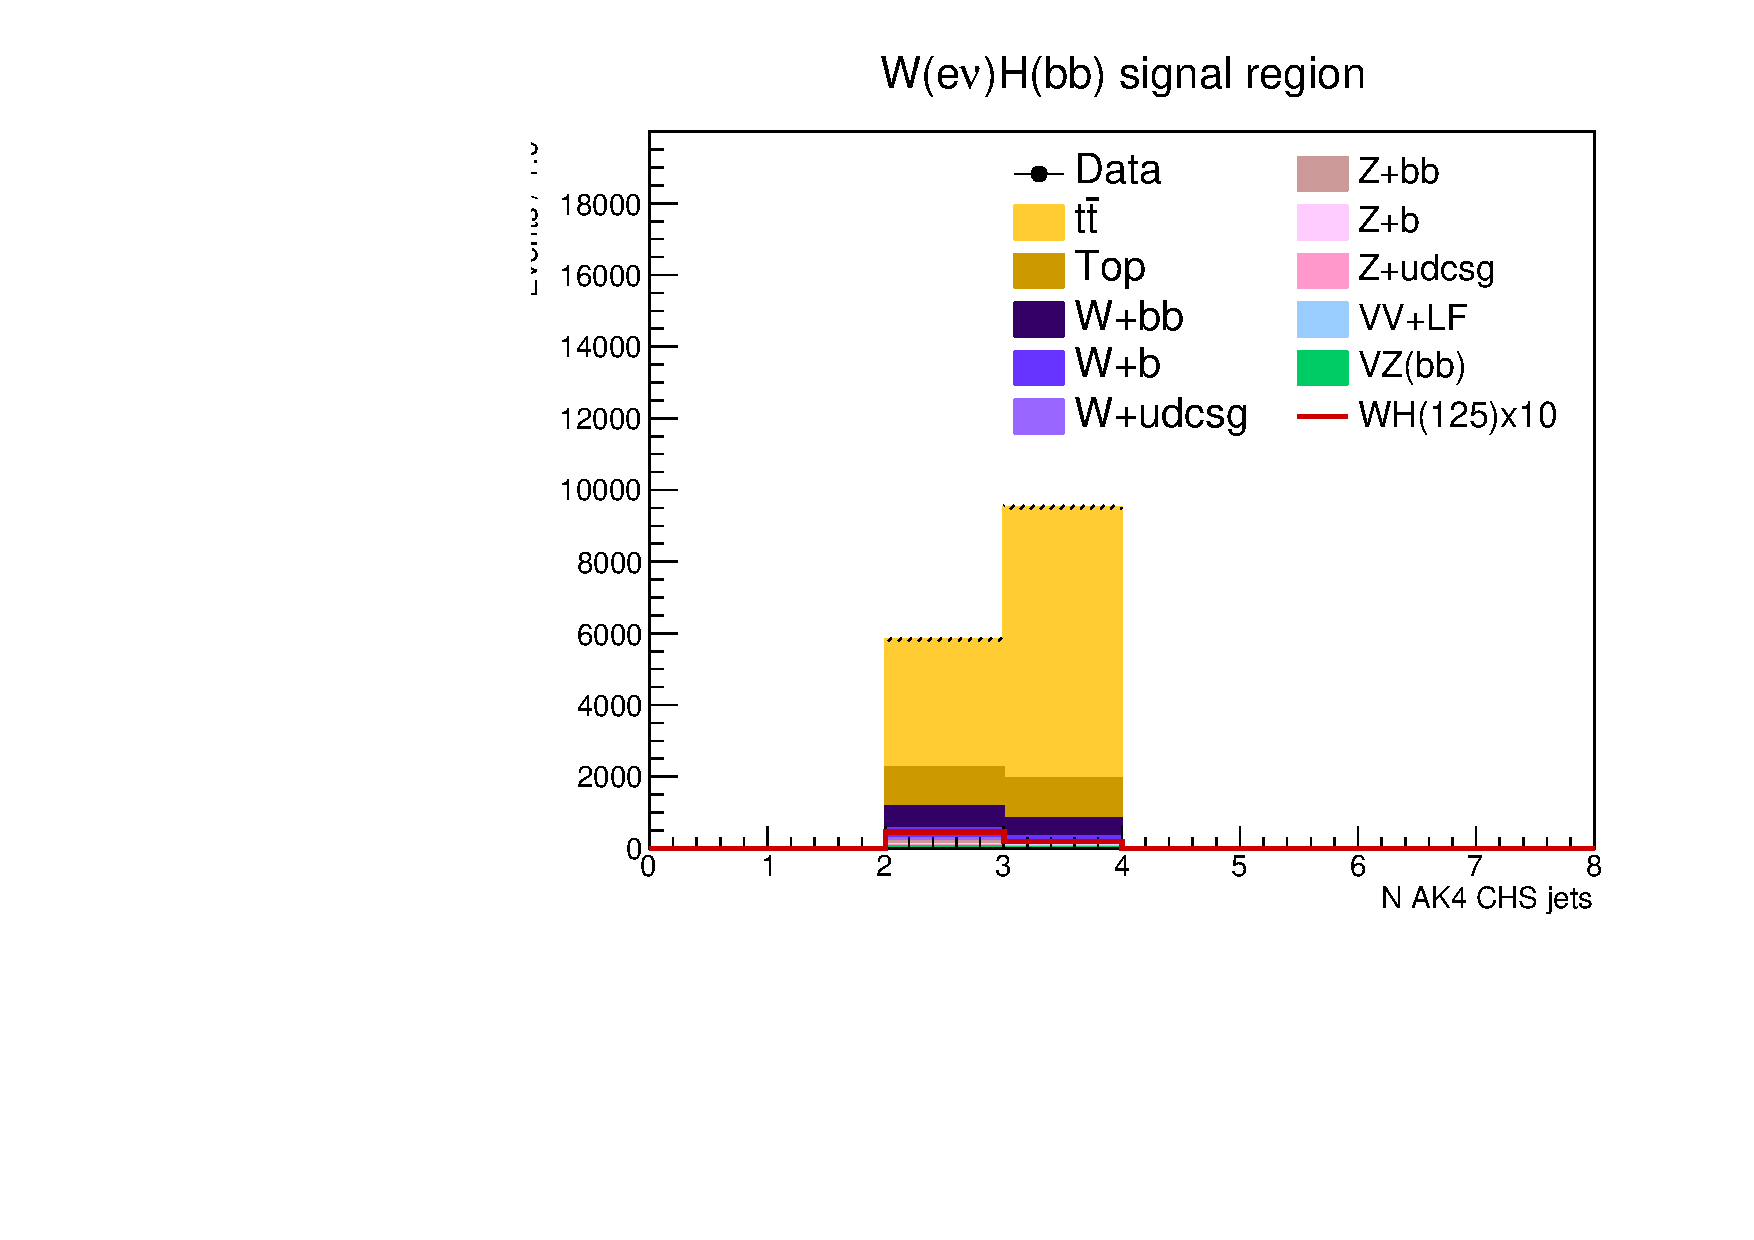
\includegraphics[width=0.48\textwidth]{figures/wlnhbb2016/resolved/WenWHSR_nJet.pdf}
    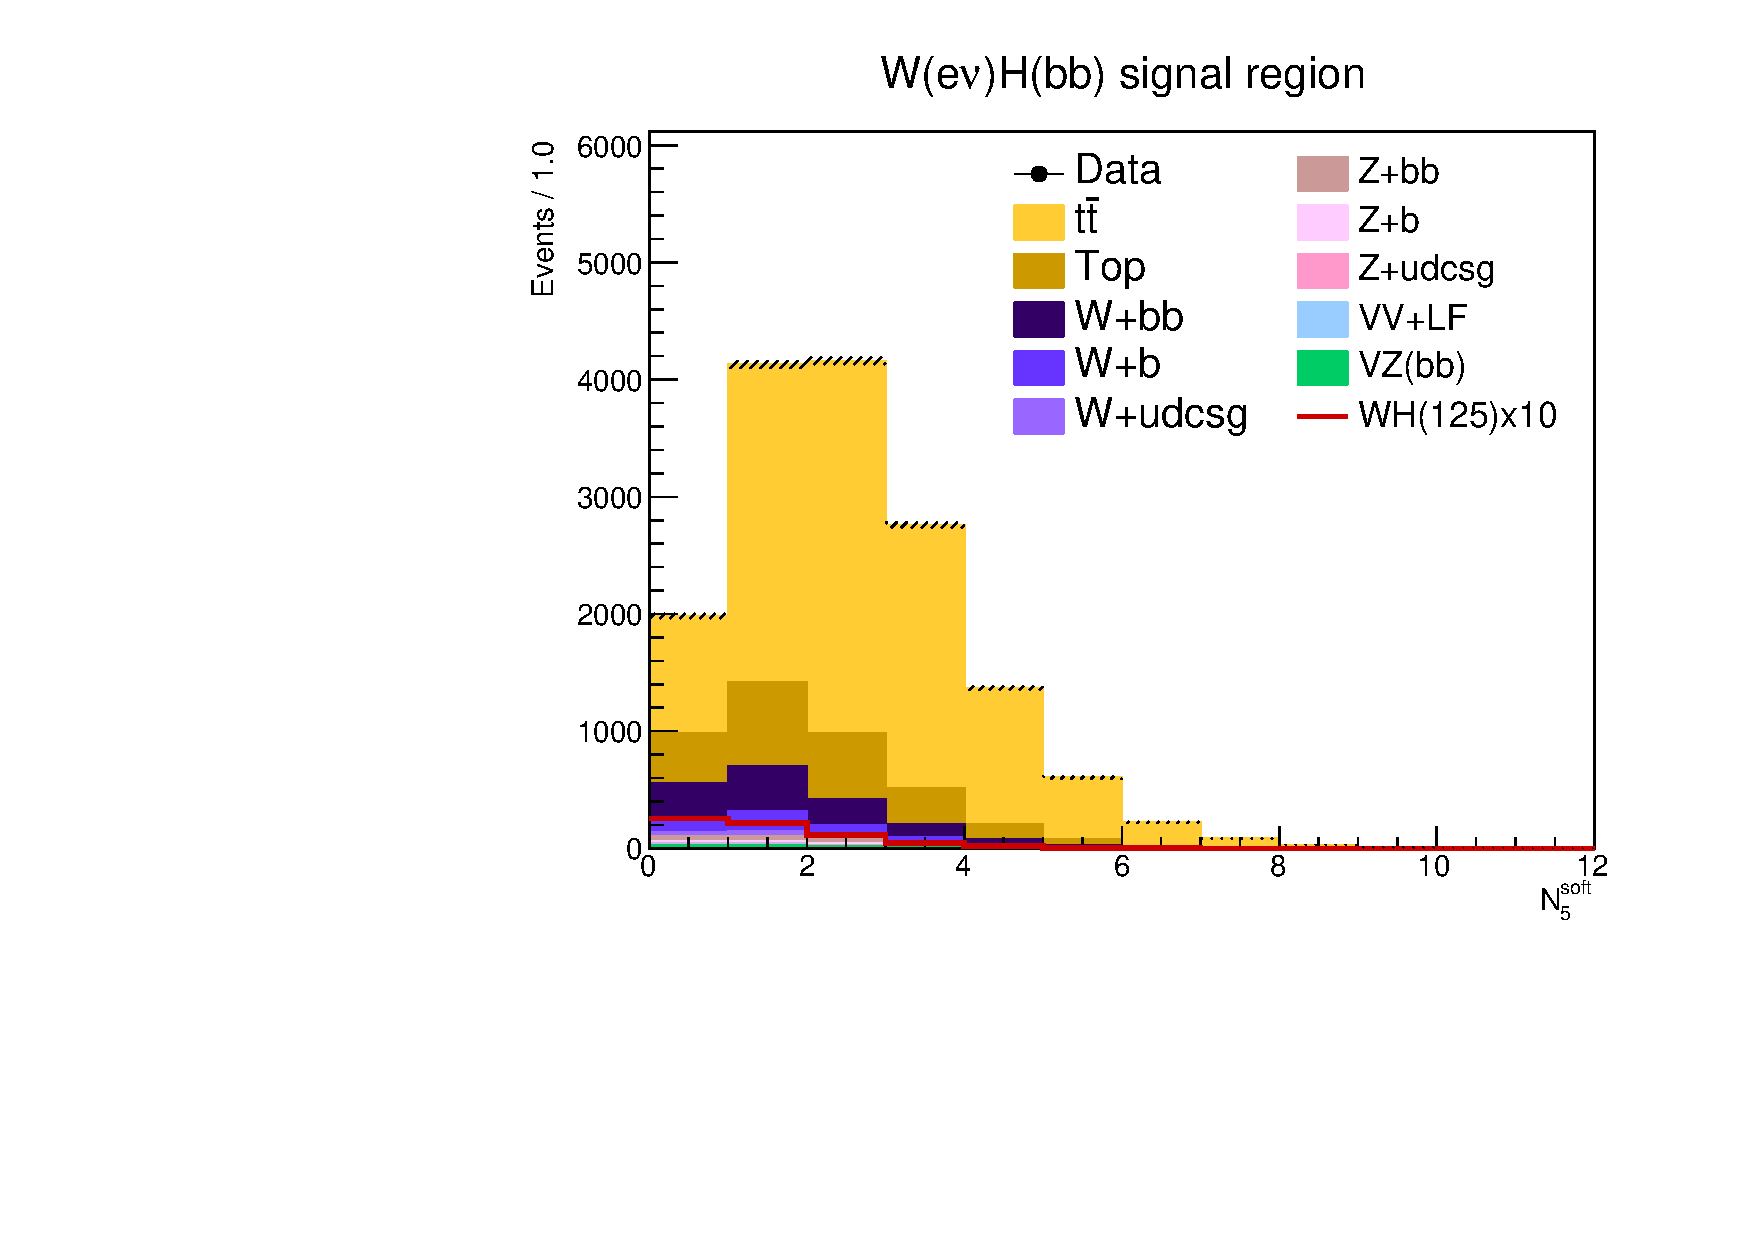
\includegraphics[width=0.48\textwidth]{figures/wlnhbb2016/resolved/WenWHSR_nSoft5.pdf}
    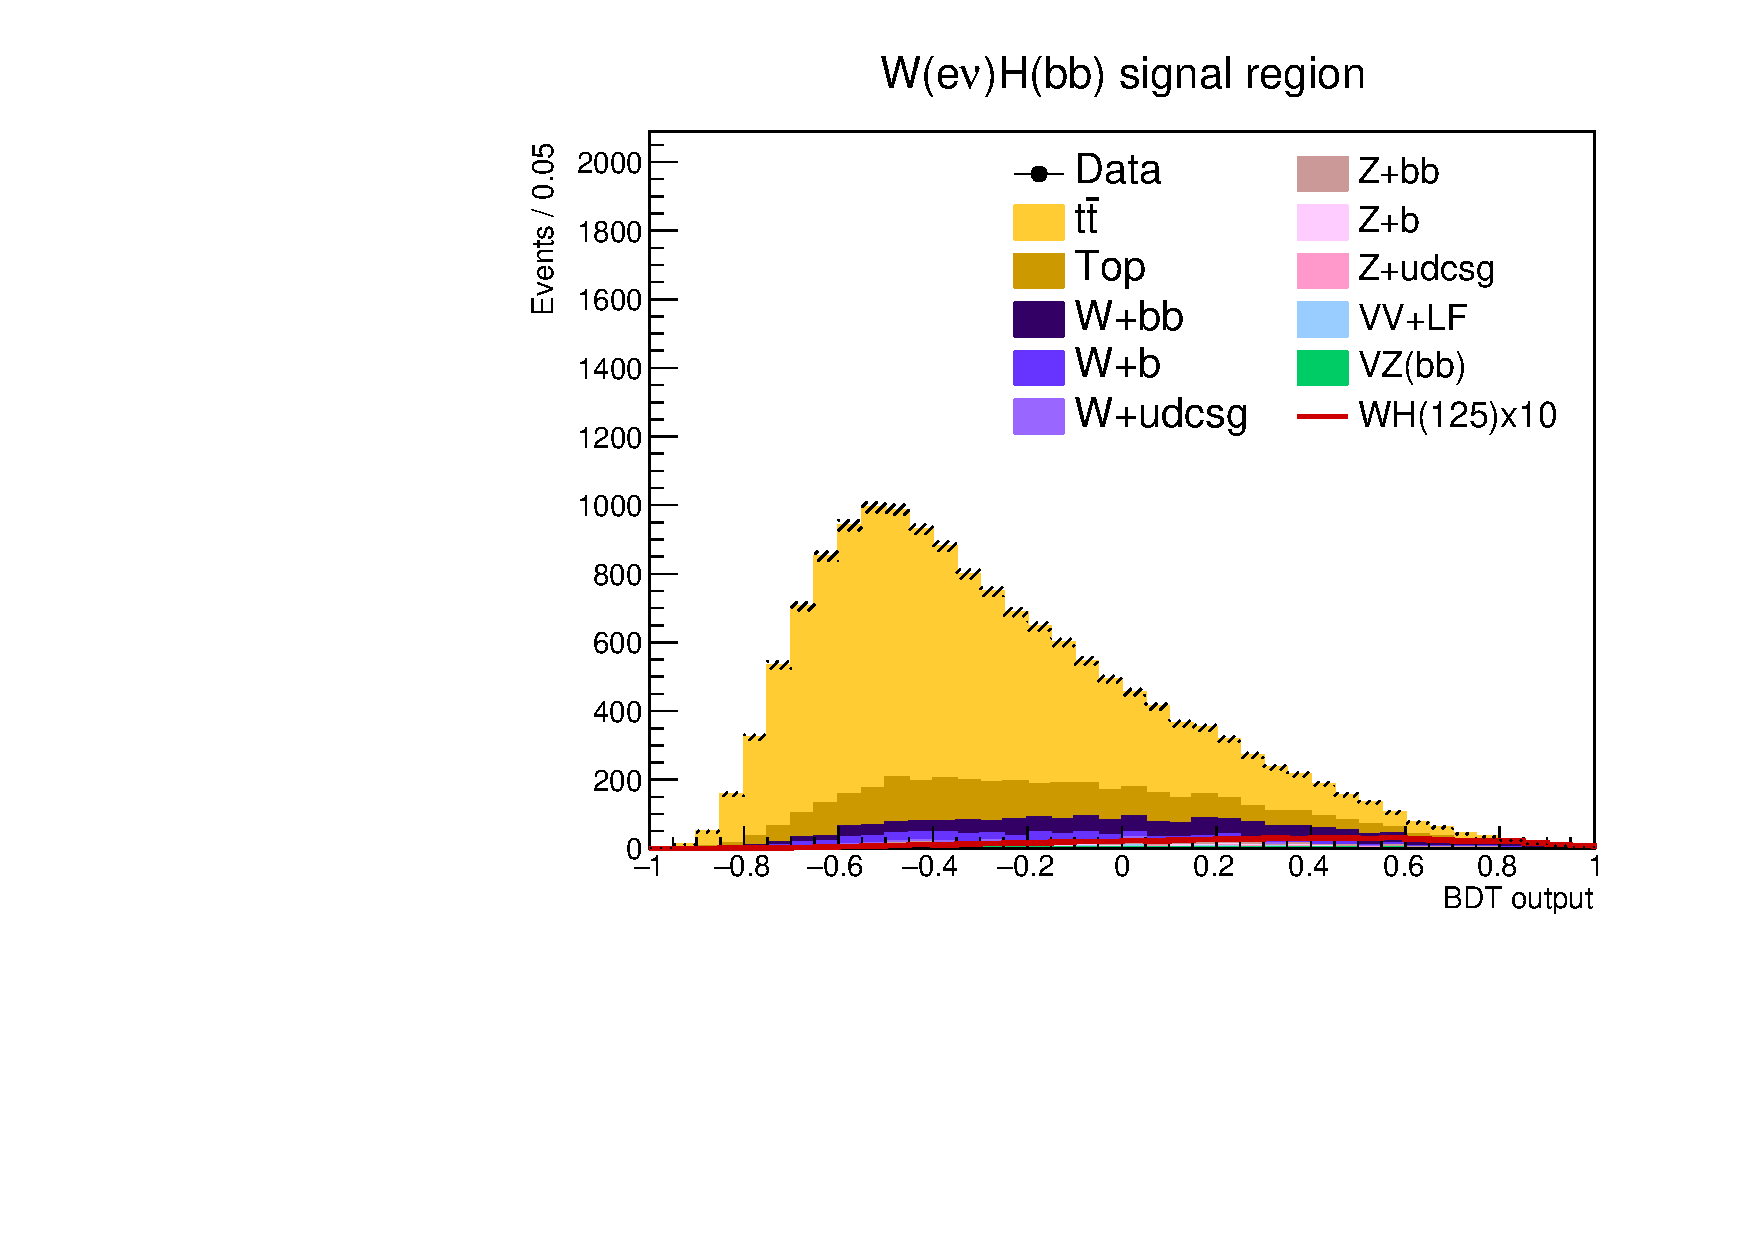
\includegraphics[width=0.48\textwidth]{figures/wlnhbb2016/resolved/WenWHSR_bdtValue.pdf}
    \caption{WH kinematics in the resolved category W(e$\nu$) signal region.
    Left to right and top to bottom: WH $\pt$ balance, WH azimuthal separation, leading b-tag score, the number of central jets,
    the number of 5 \GeV\ soft activity jets, and the evaluation of the signal extraction BDT.
    The simulated shapes are prefit, with the postfit normalizations applied.}
    \label{fig:res_WenSR_WH}
  \end{center}
\end{figure}
\clearpage


\begin{figure}[tbp]
  \begin{center}
    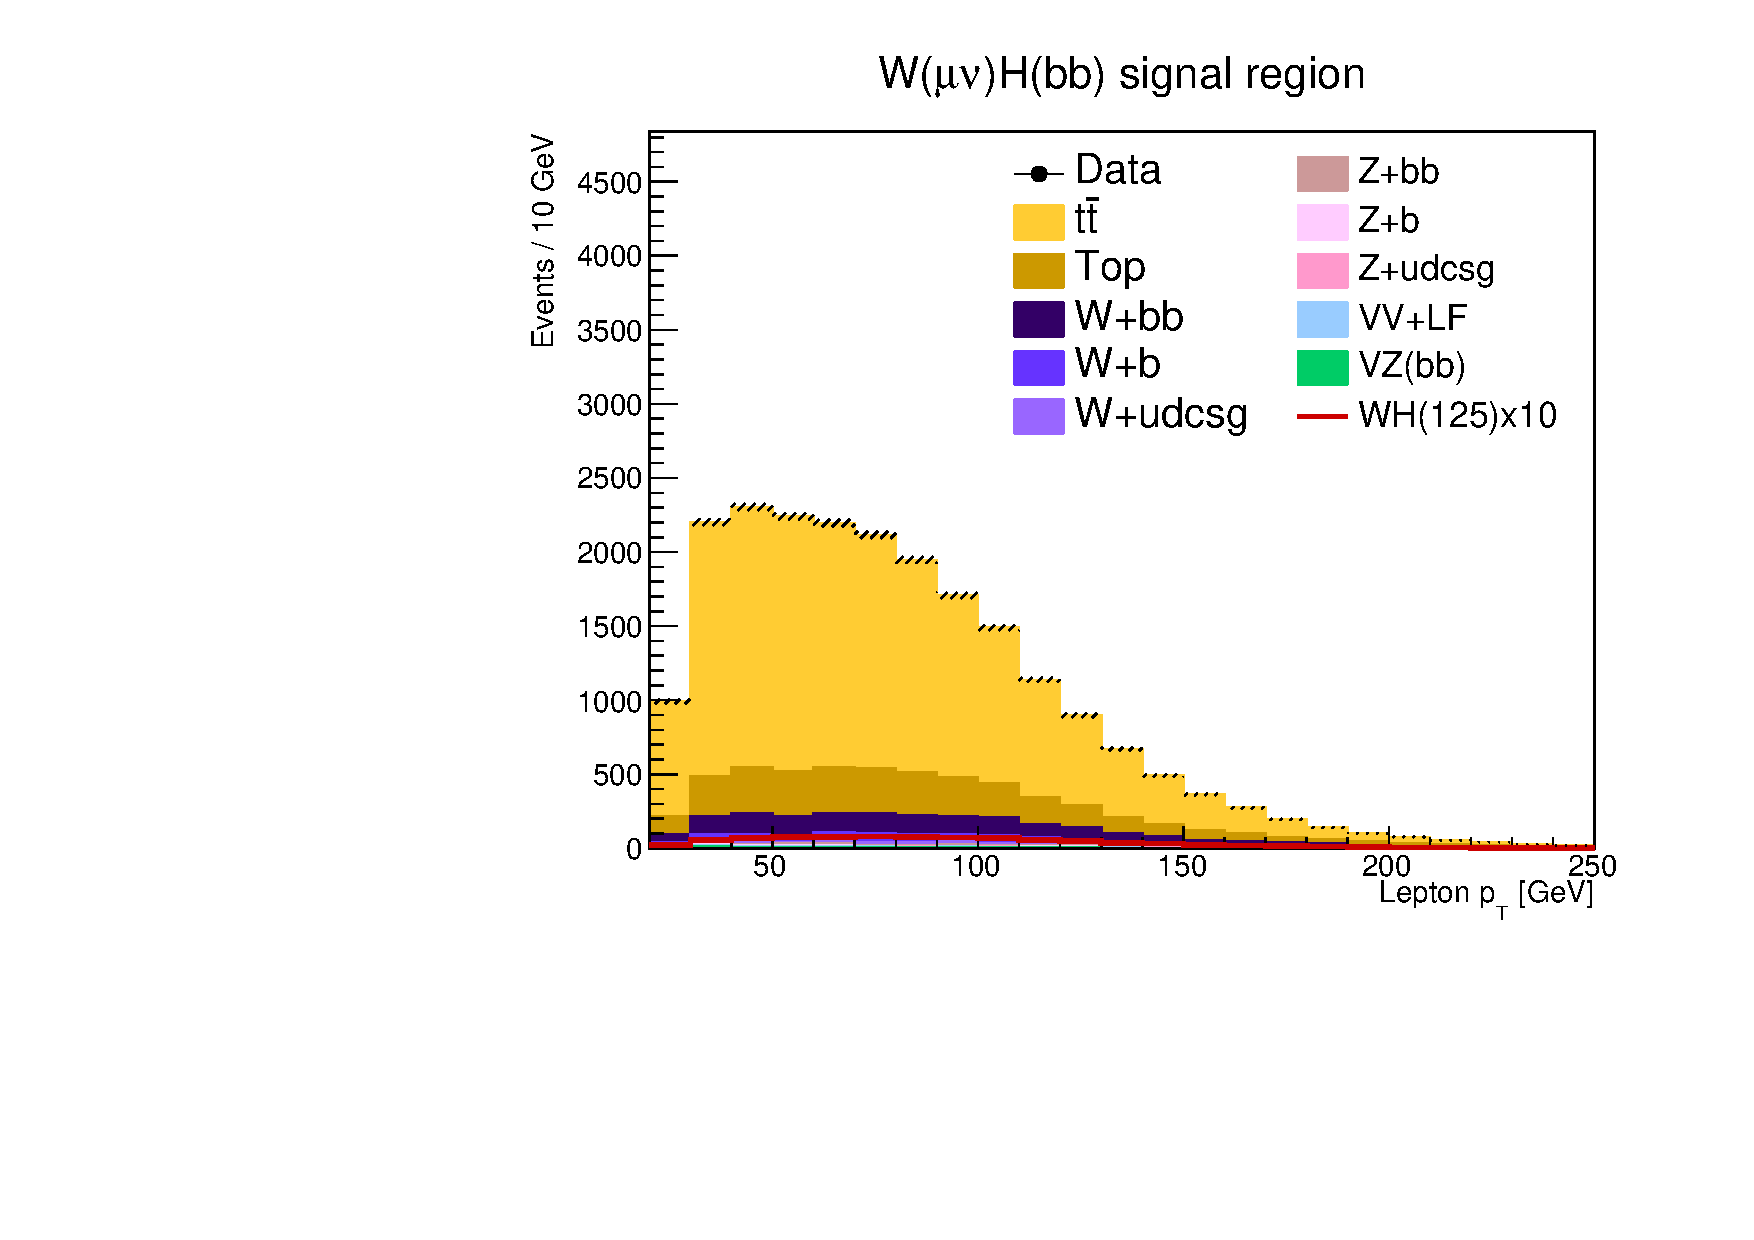
\includegraphics[width=0.48\textwidth]{figures/wlnhbb2016/resolved/WmnWHSR_lepton1Pt.pdf}
    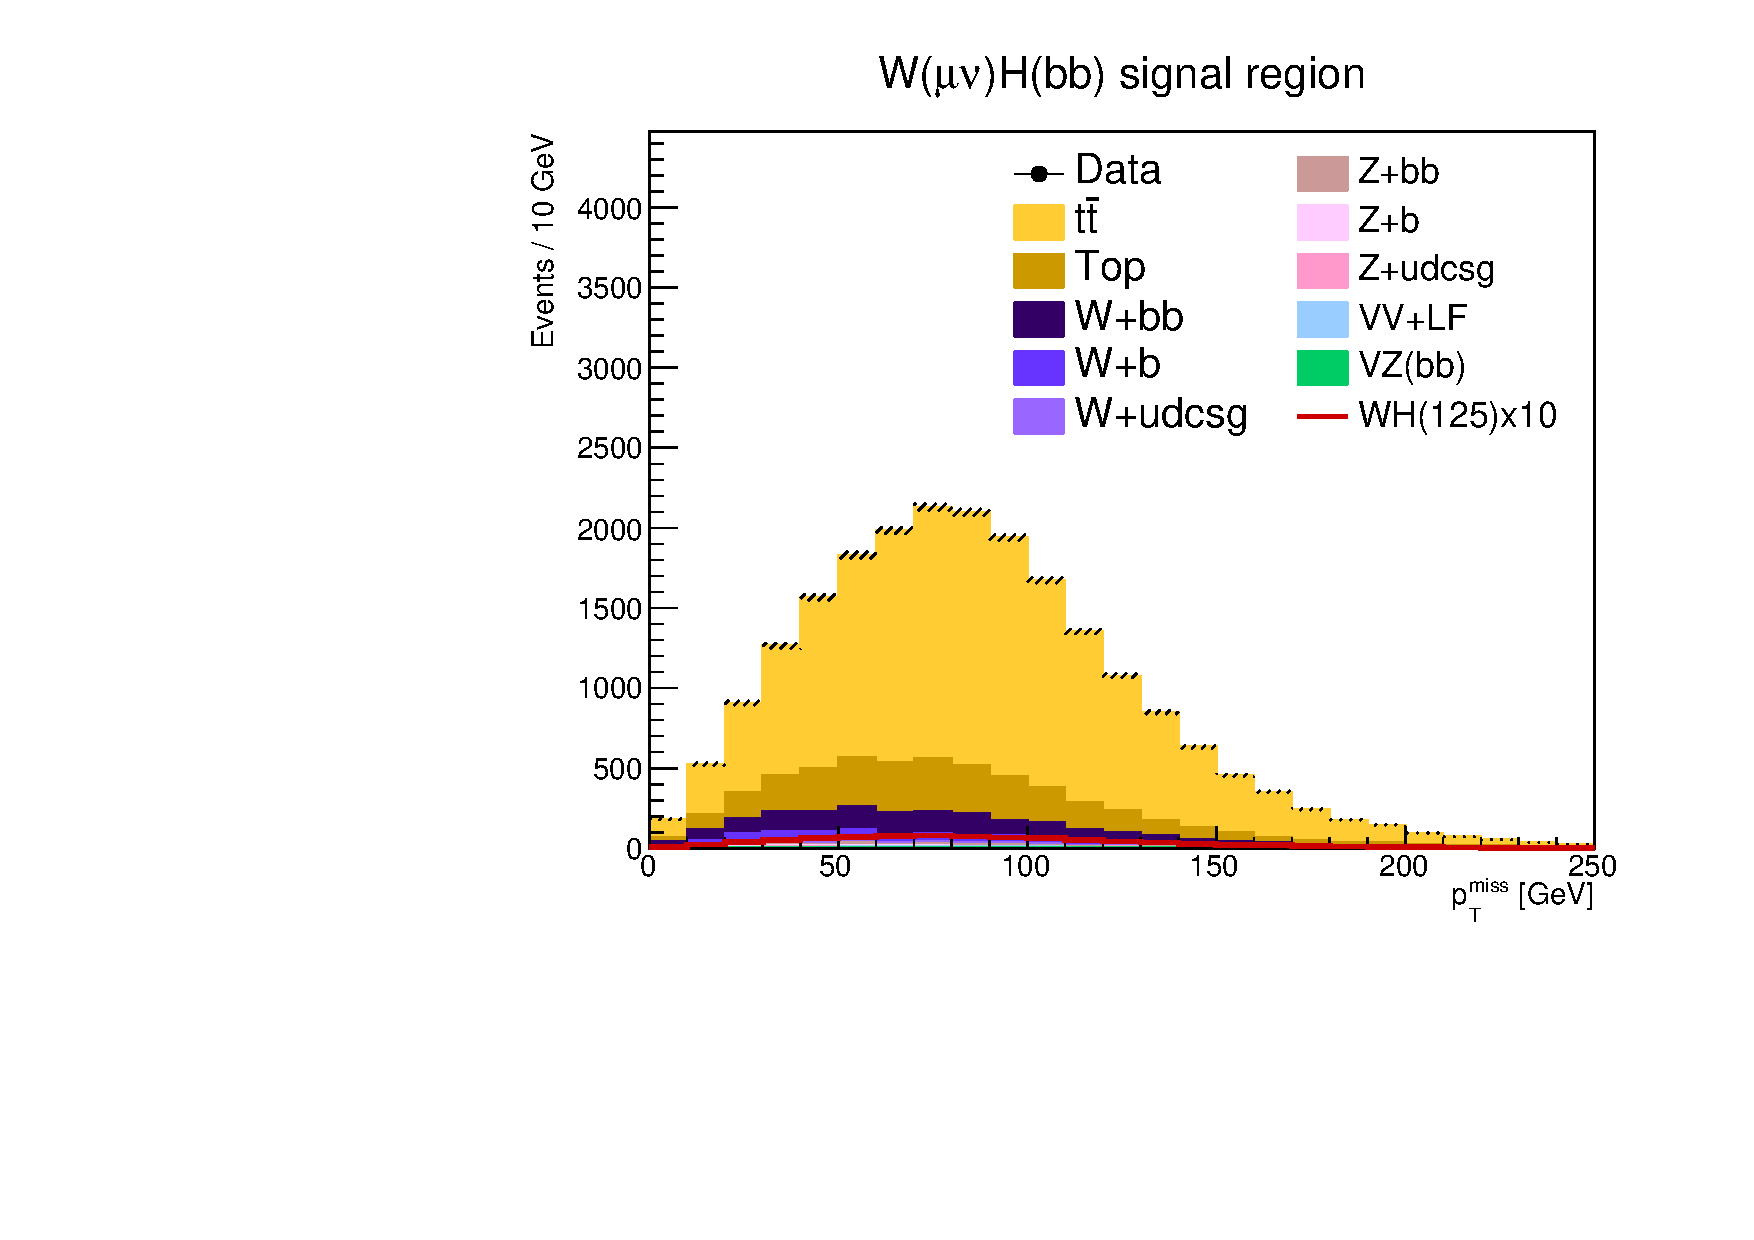
\includegraphics[width=0.48\textwidth]{figures/wlnhbb2016/resolved/WmnWHSR_pfmet.pdf}
    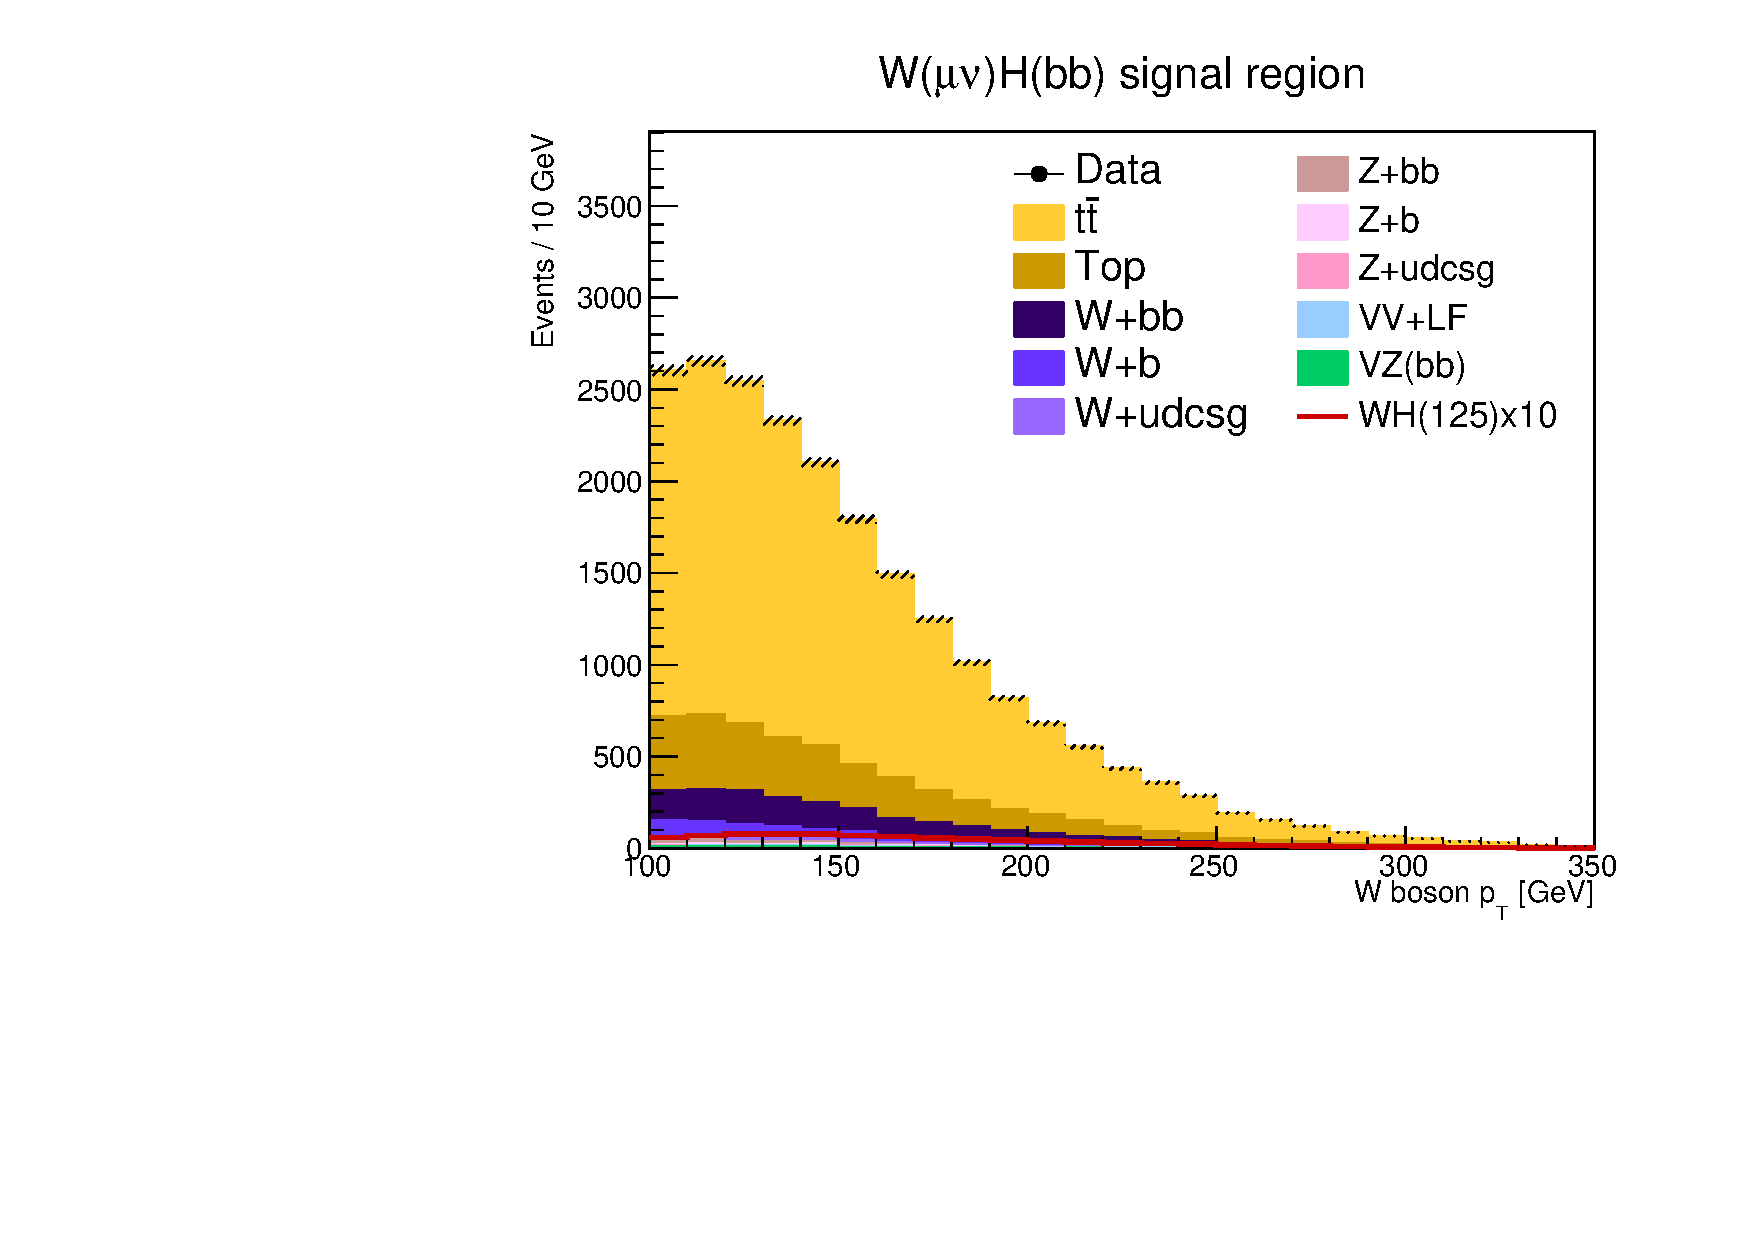
\includegraphics[width=0.48\textwidth]{figures/wlnhbb2016/resolved/WmnWHSR_WpT.pdf}
    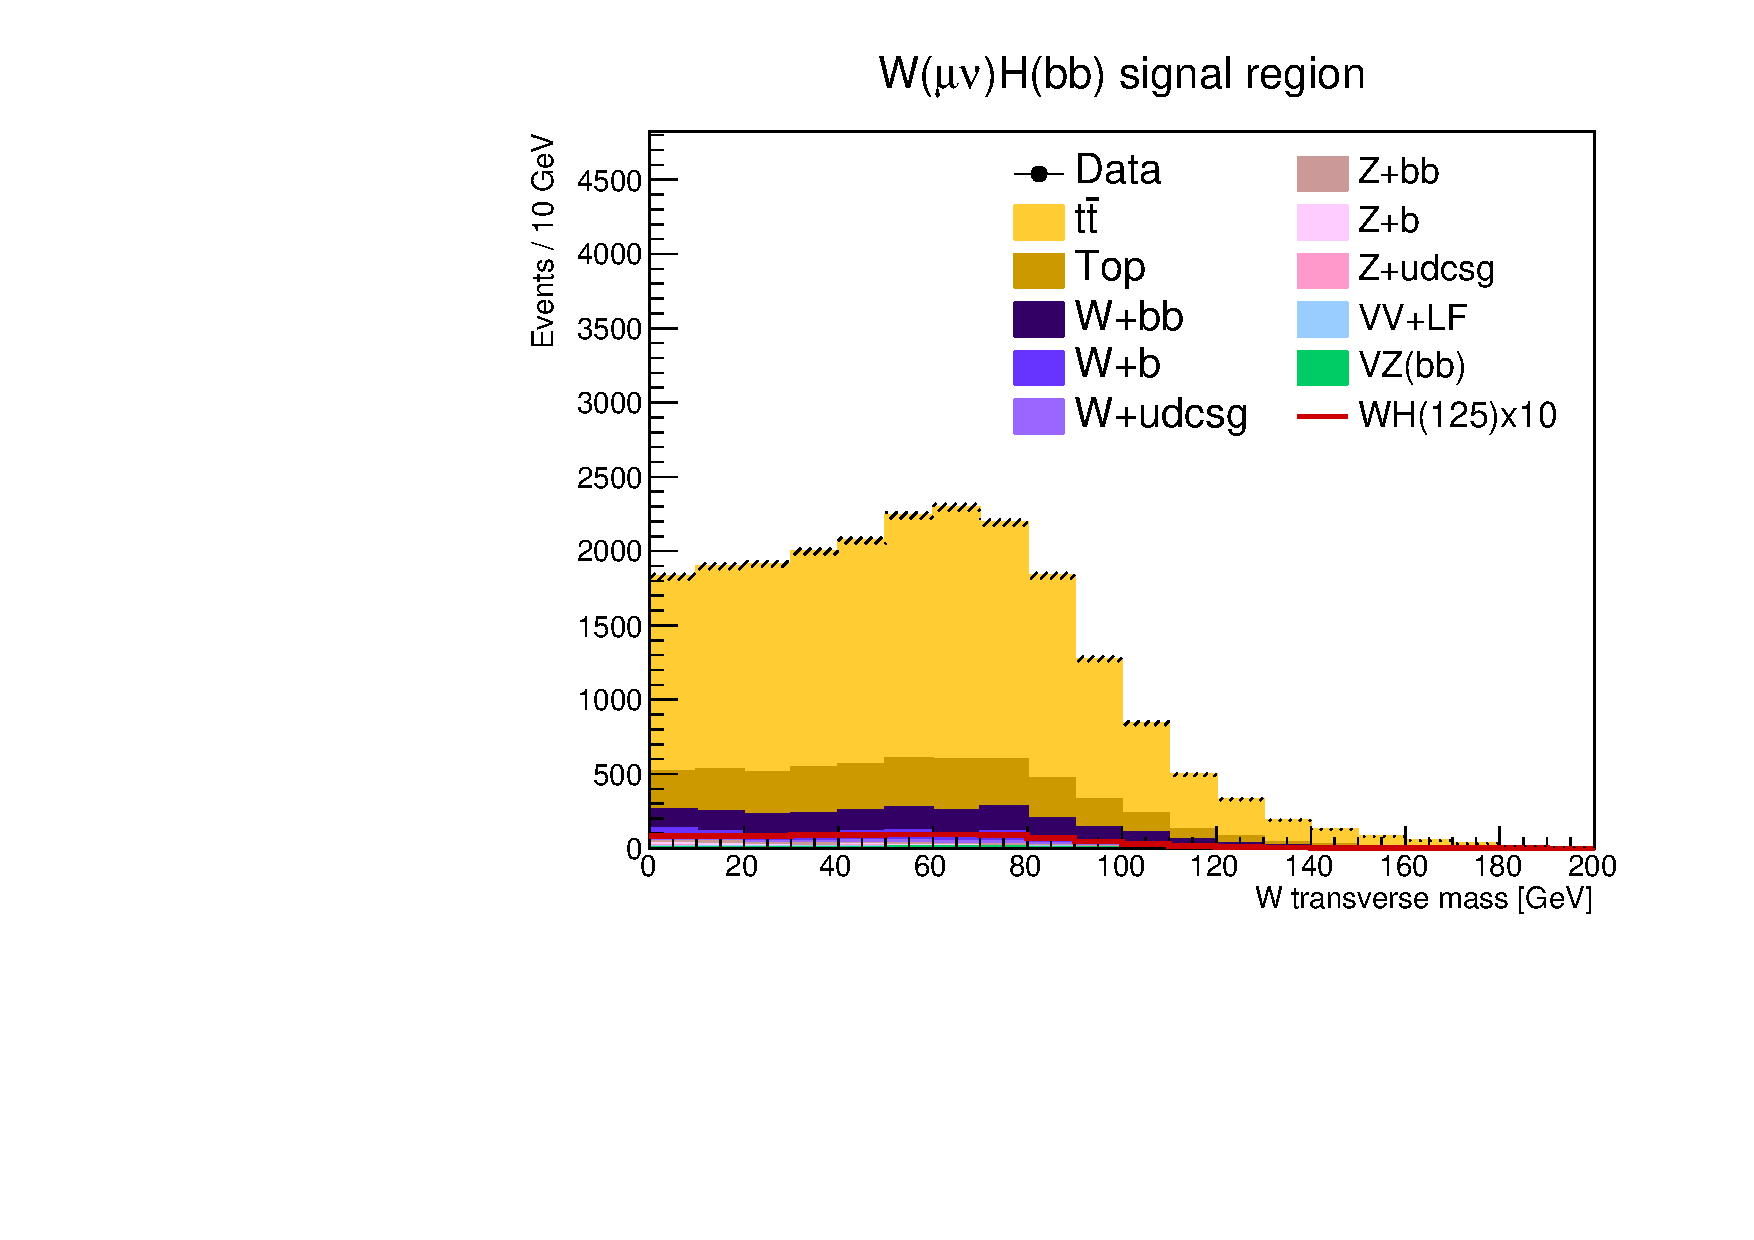
\includegraphics[width=0.48\textwidth]{figures/wlnhbb2016/resolved/WmnWHSR_mTW.pdf}
    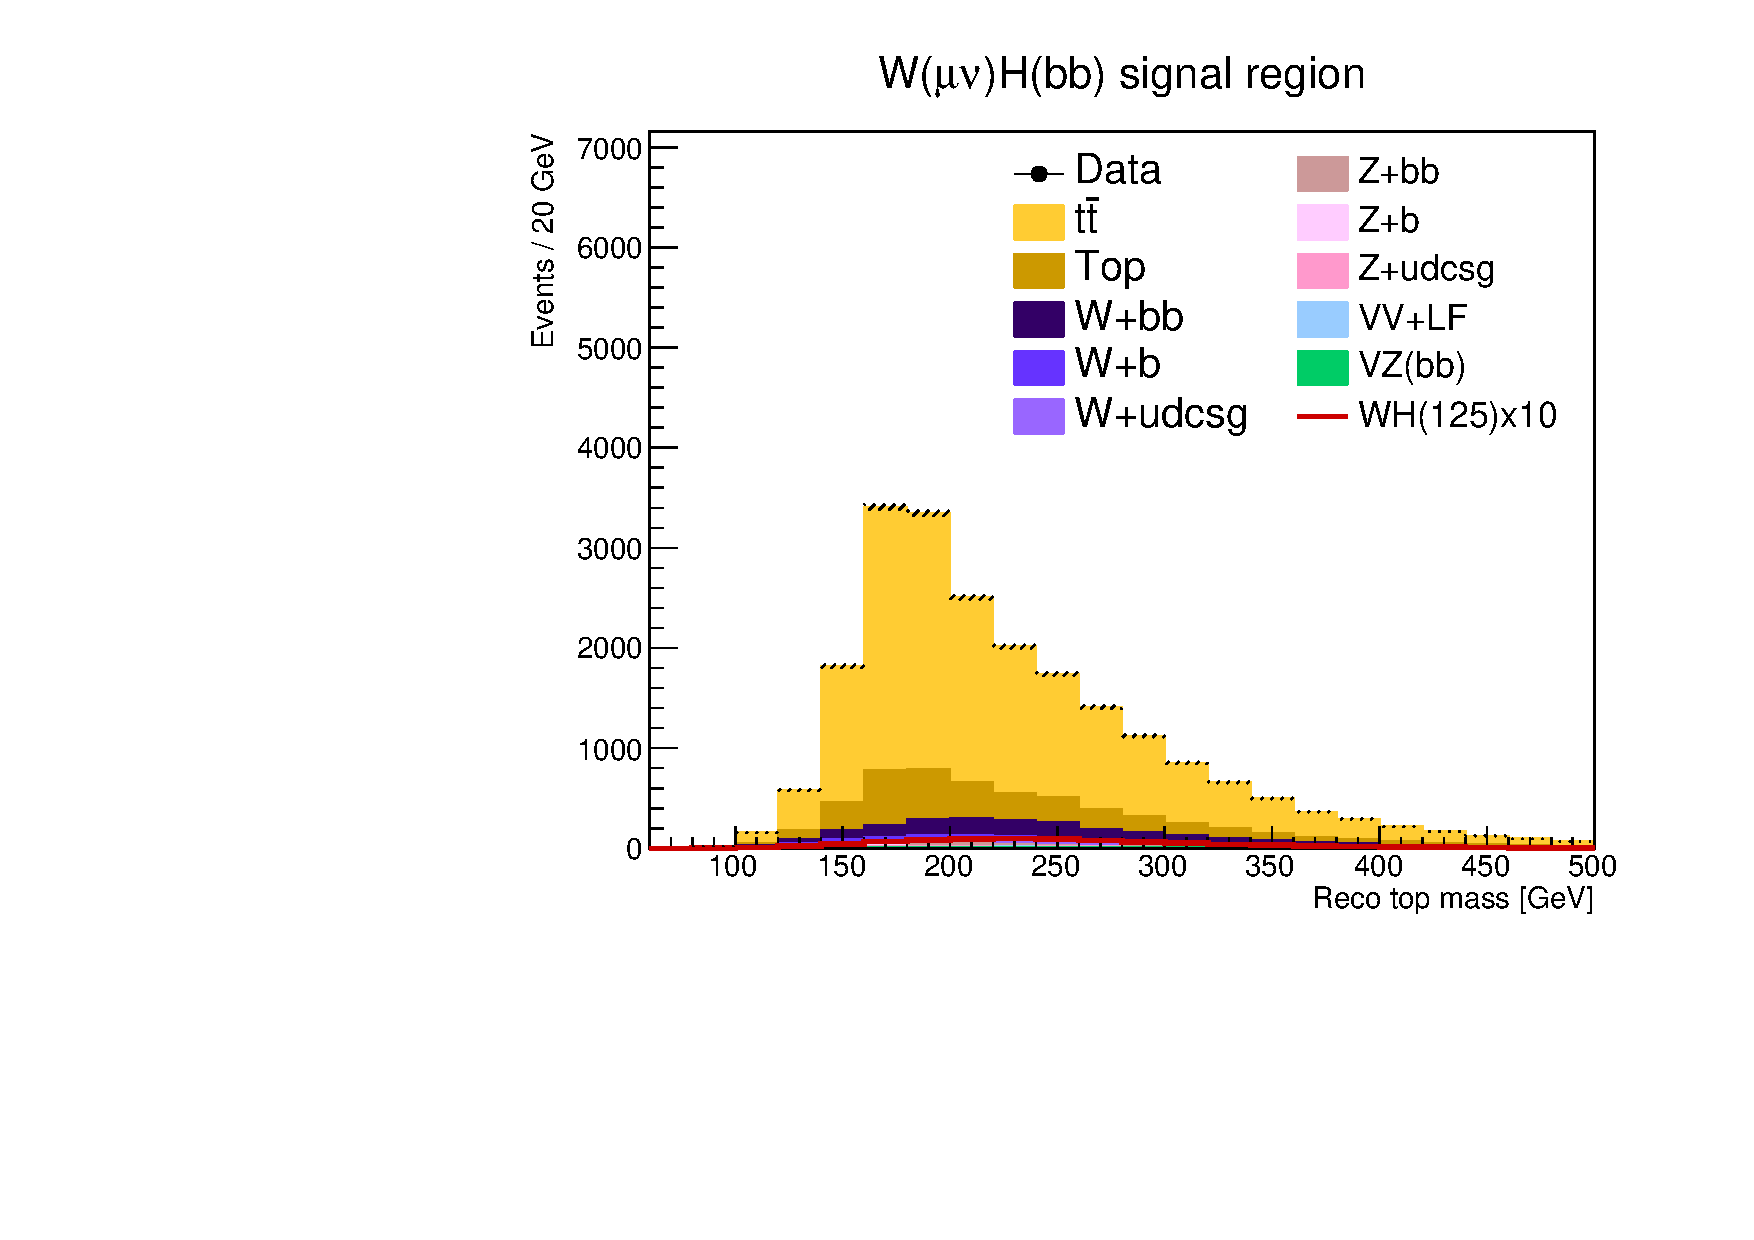
\includegraphics[width=0.48\textwidth]{figures/wlnhbb2016/resolved/WmnWHSR_topMassLep1Met.pdf}
    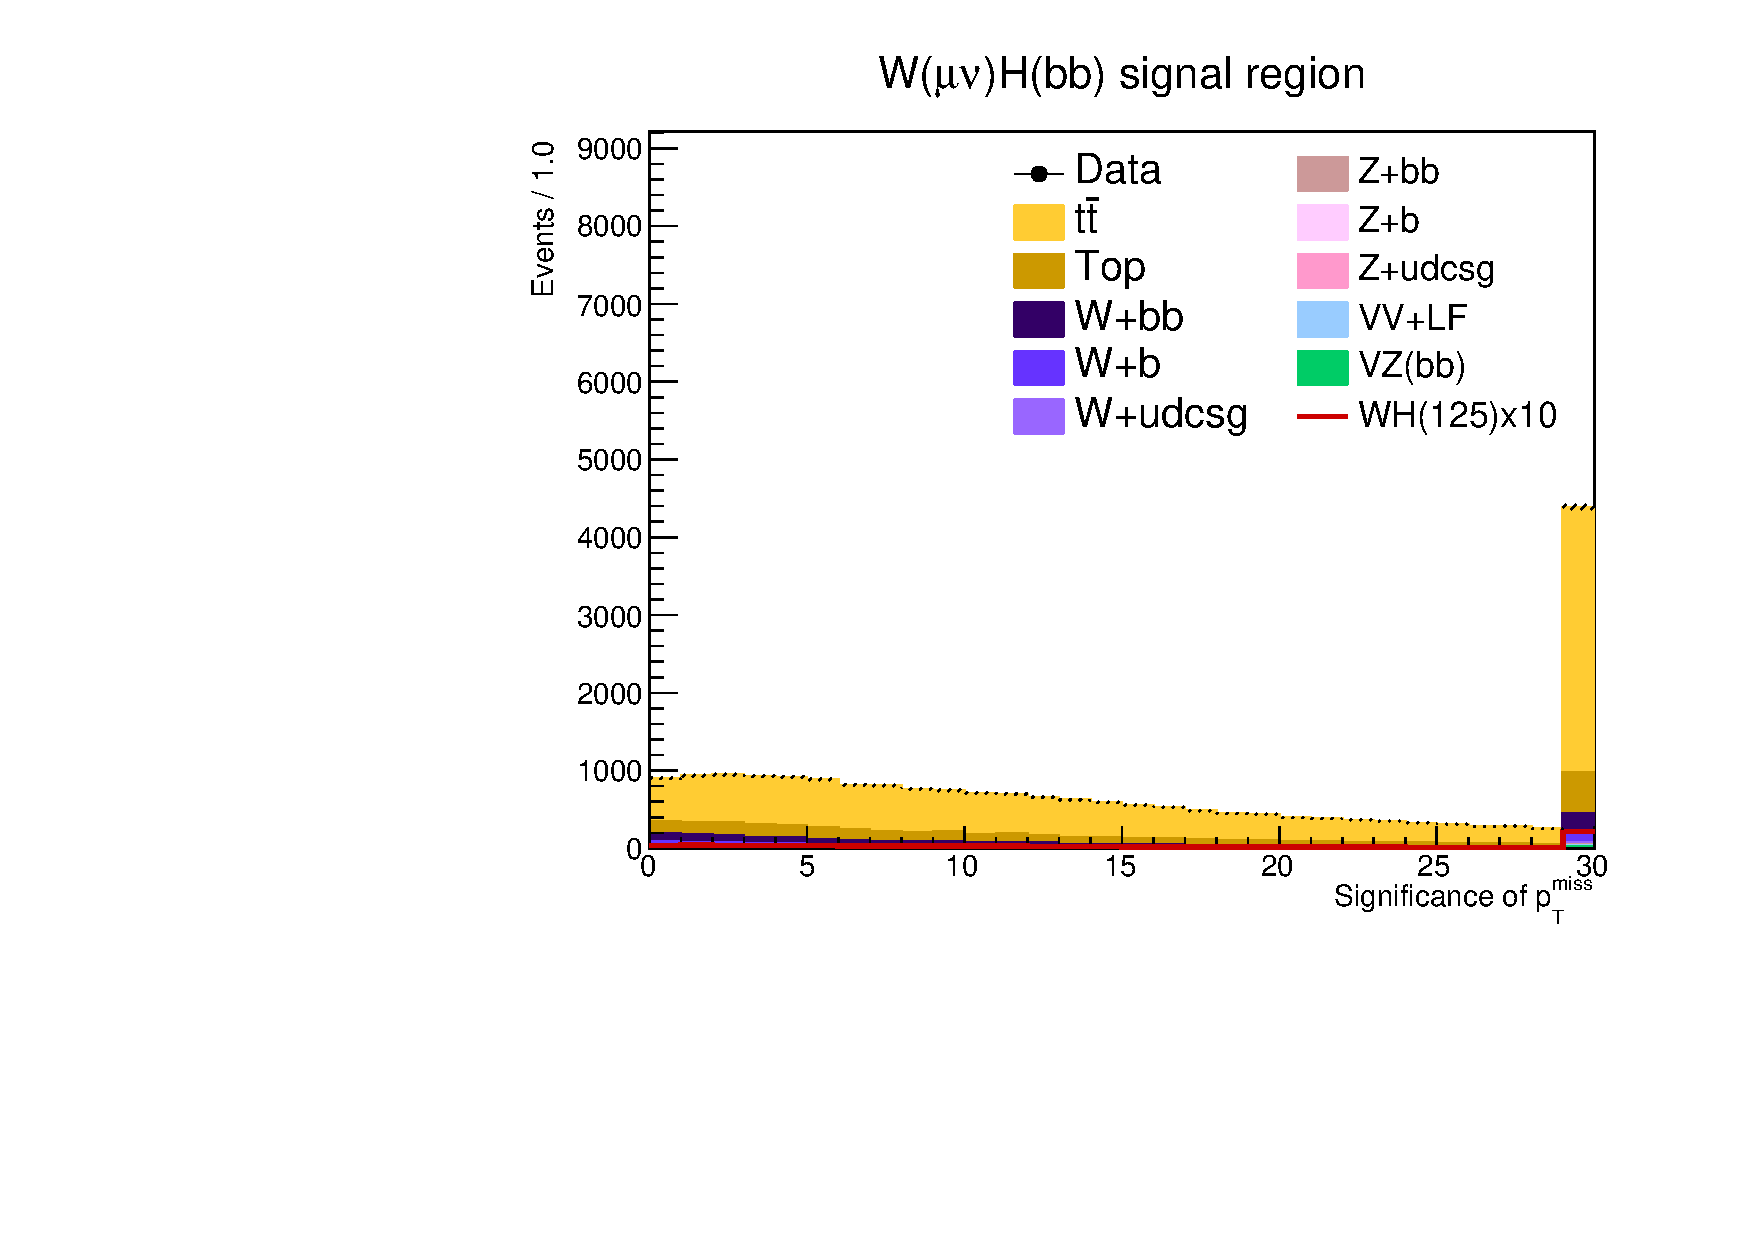
\includegraphics[width=0.48\textwidth]{figures/wlnhbb2016/resolved/WmnWHSR_pfmetsig.pdf}
    \caption{W boson reconstruction in the resolved category W($\mu\nu$) signal region.
    Left to right and top to bottom: muon $\pt$, $\MET$, W boson $\pt$, W boson transverse mass,
    the reconstructed top quark mass, and the $\MET$ significance.
    The simulated shapes are prefit, with the postfit normalizations applied.}
    \label{fig:res_WmnSR_WBosons}
  \end{center}
\end{figure}
\clearpage

\begin{figure}[tbp]
  \begin{center}
    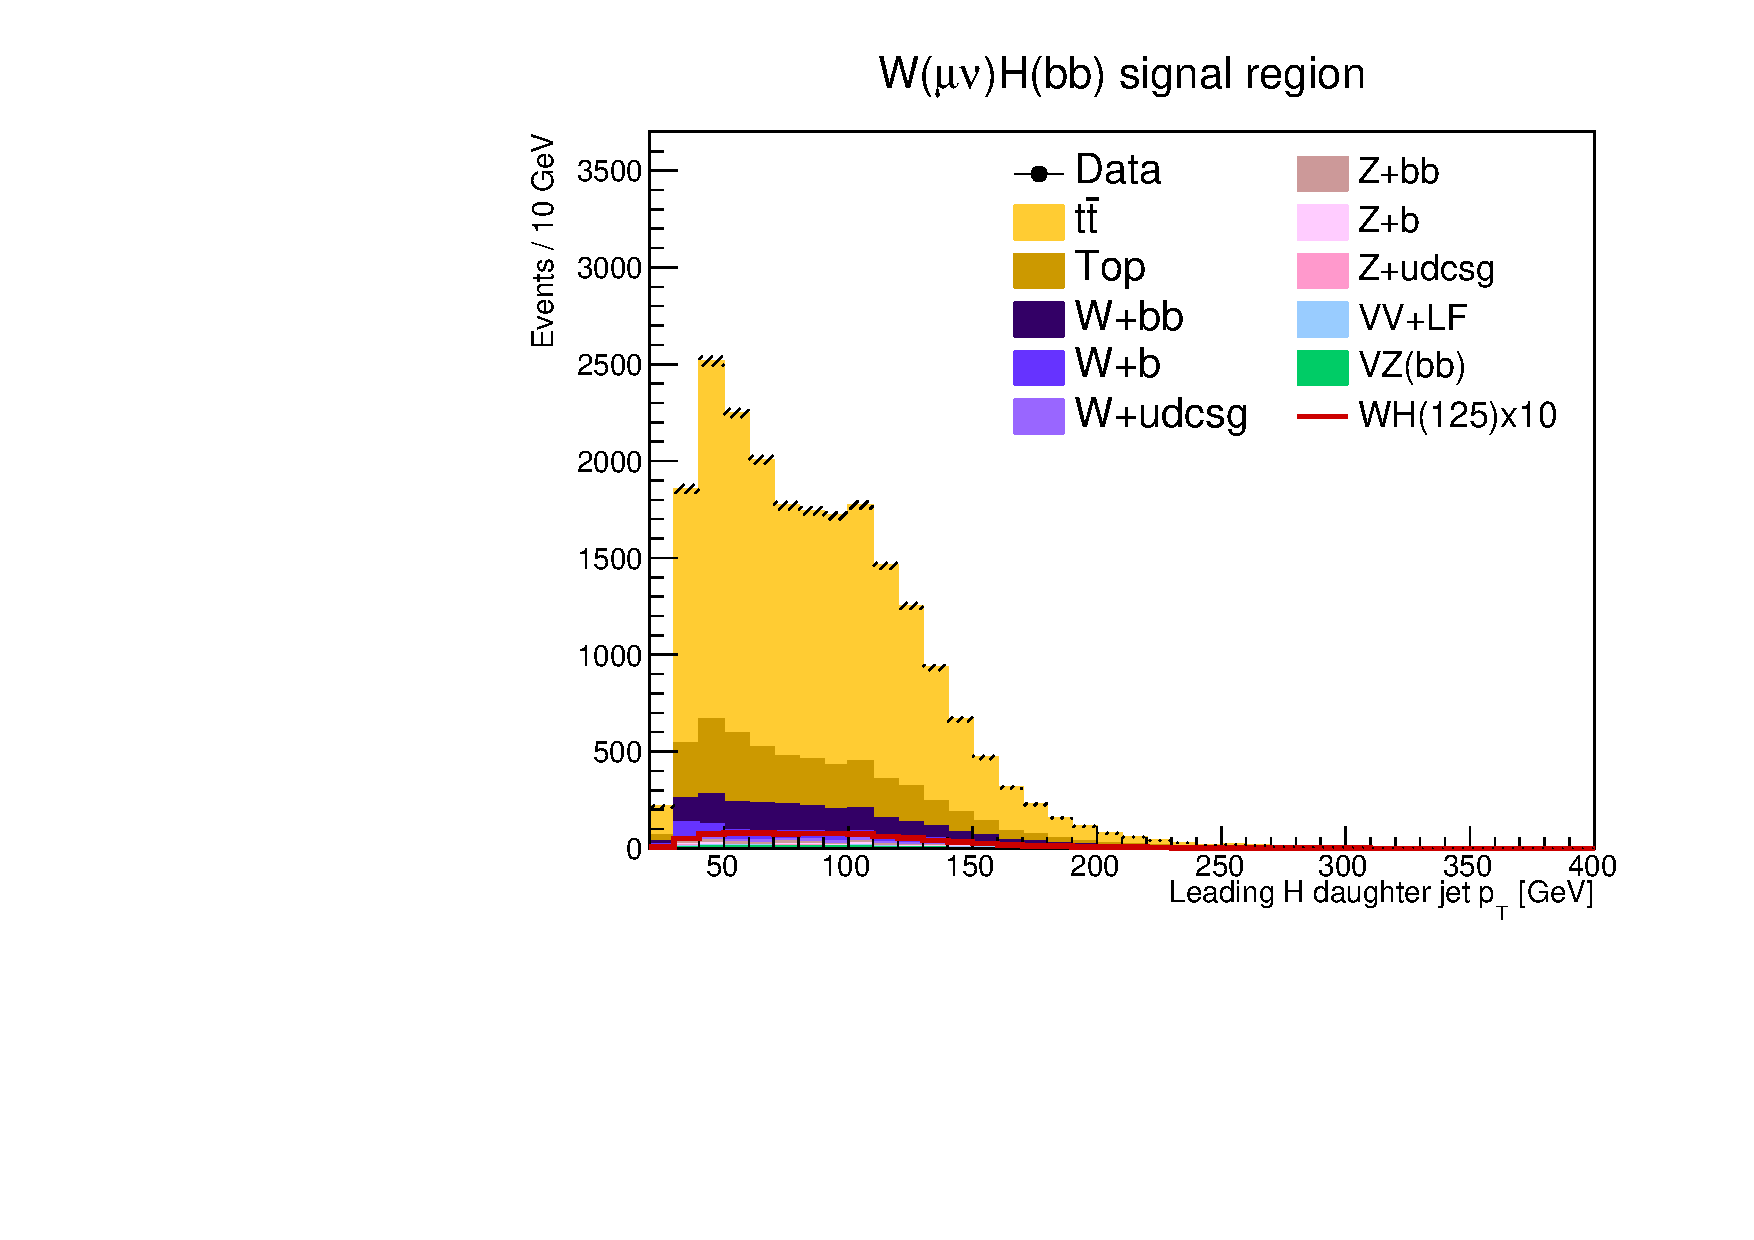
\includegraphics[width=0.48\textwidth]{figures/wlnhbb2016/resolved/WmnWHSR_Hbjet1Pt.pdf}
    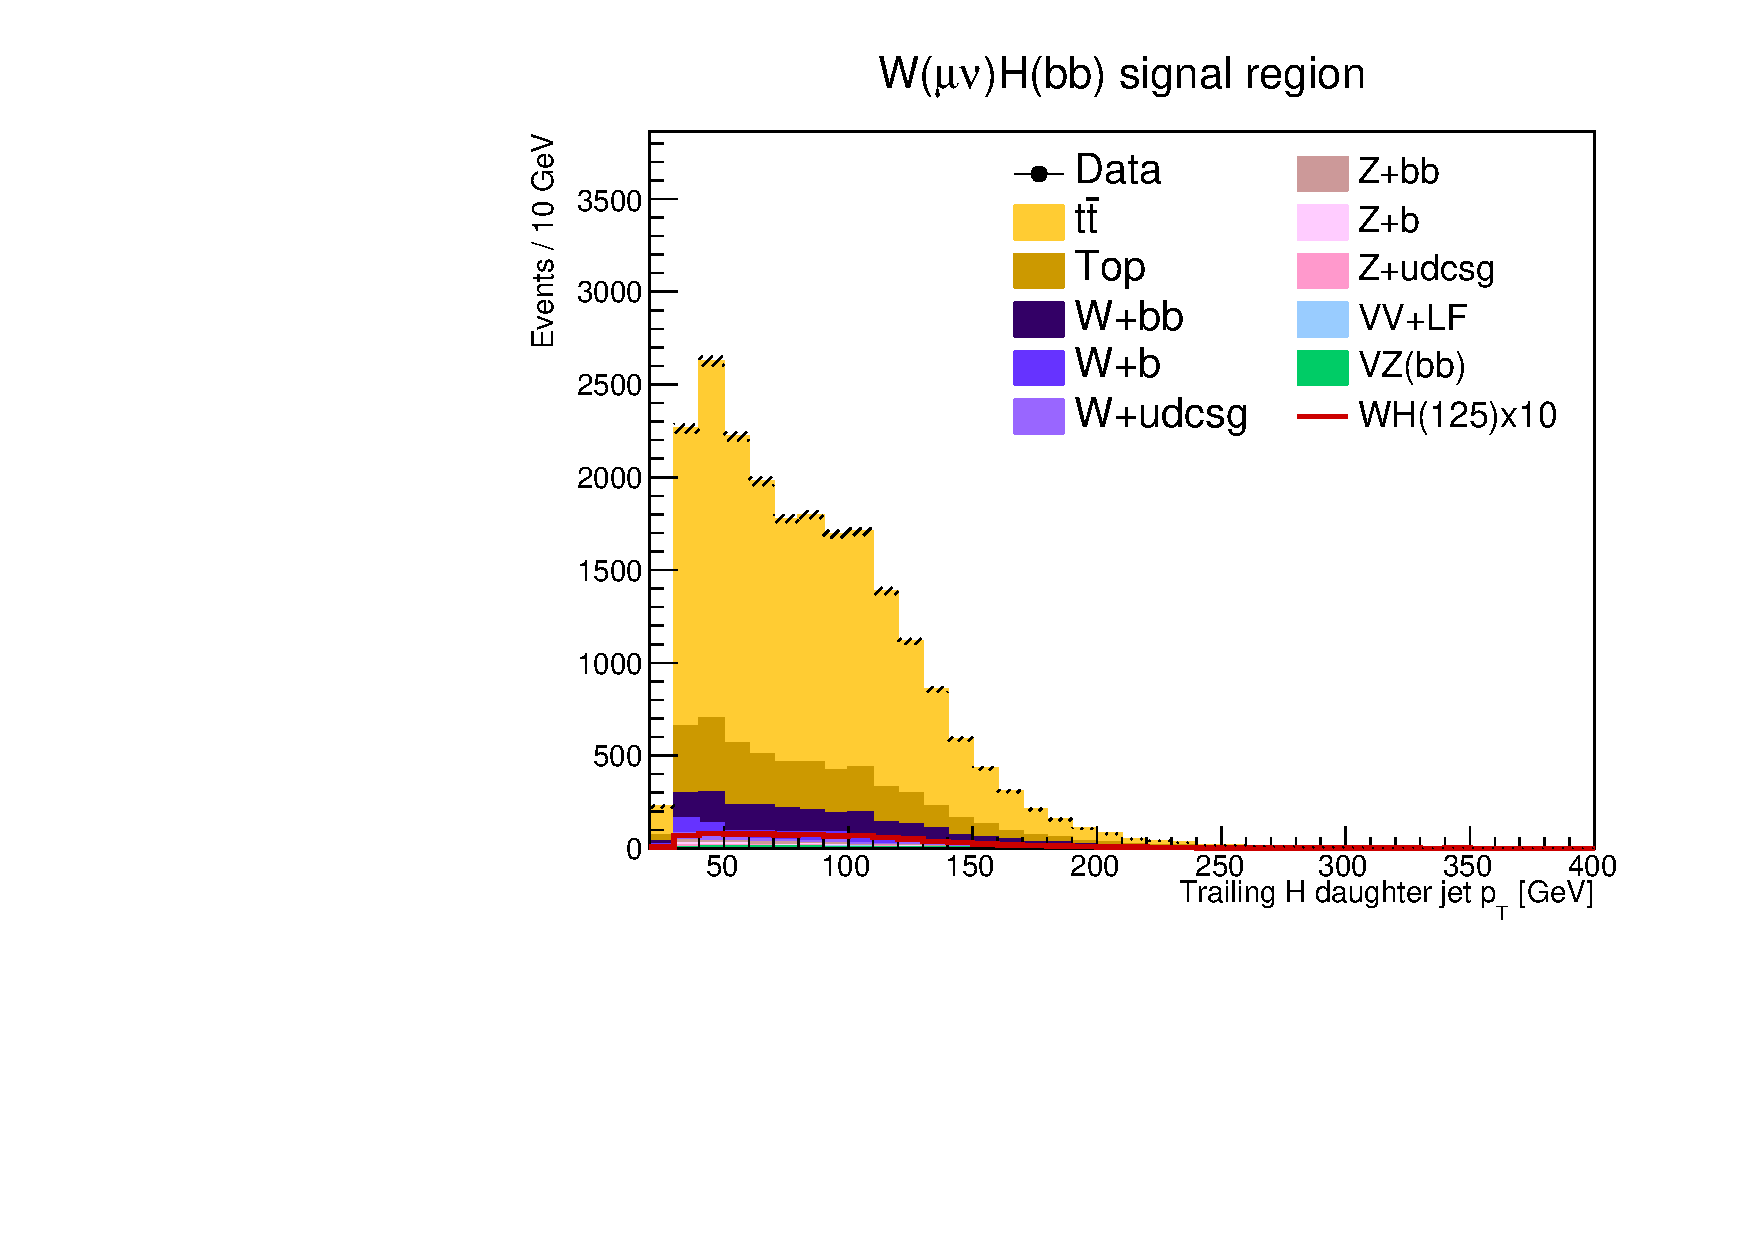
\includegraphics[width=0.48\textwidth]{figures/wlnhbb2016/resolved/WmnWHSR_Hbjet2Pt.pdf}
    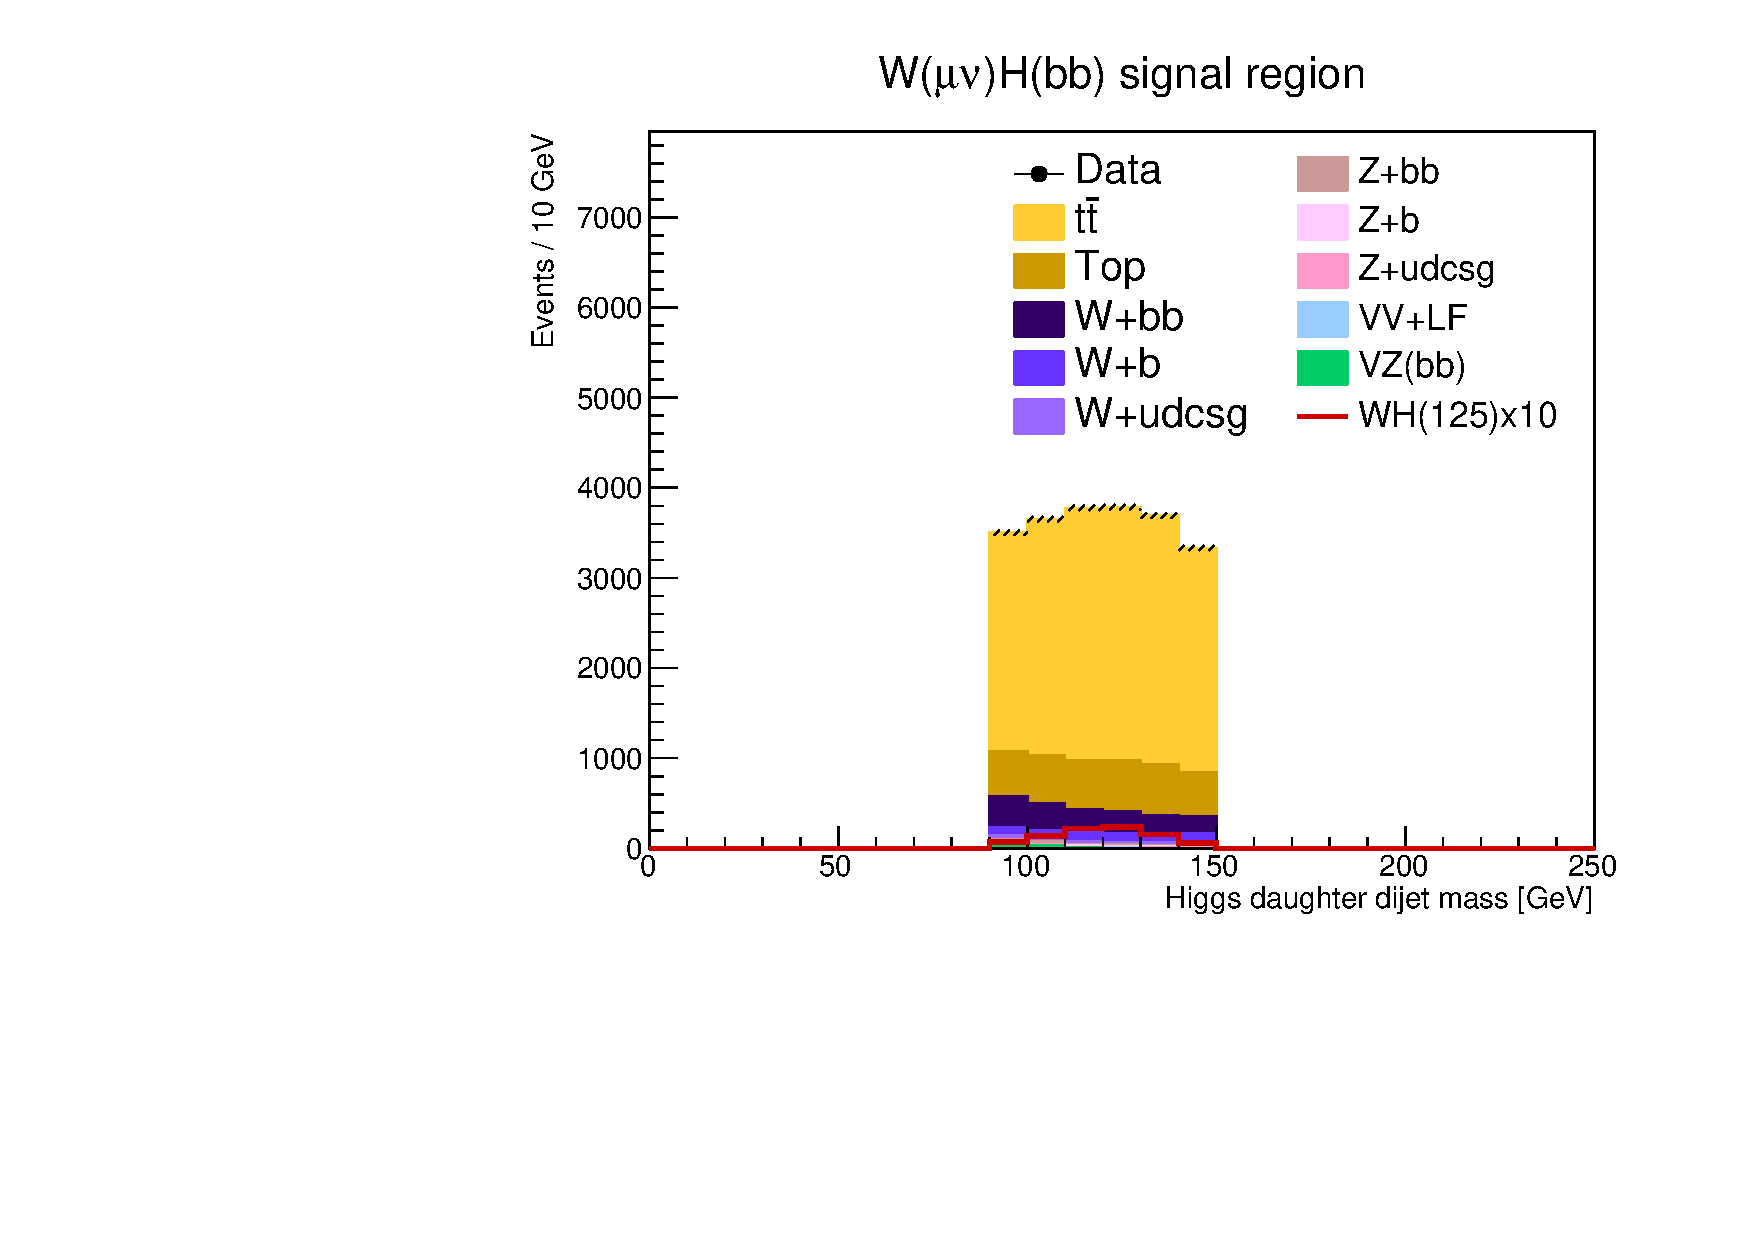
\includegraphics[width=0.48\textwidth]{figures/wlnhbb2016/resolved/WmnWHSR_mH.pdf}
    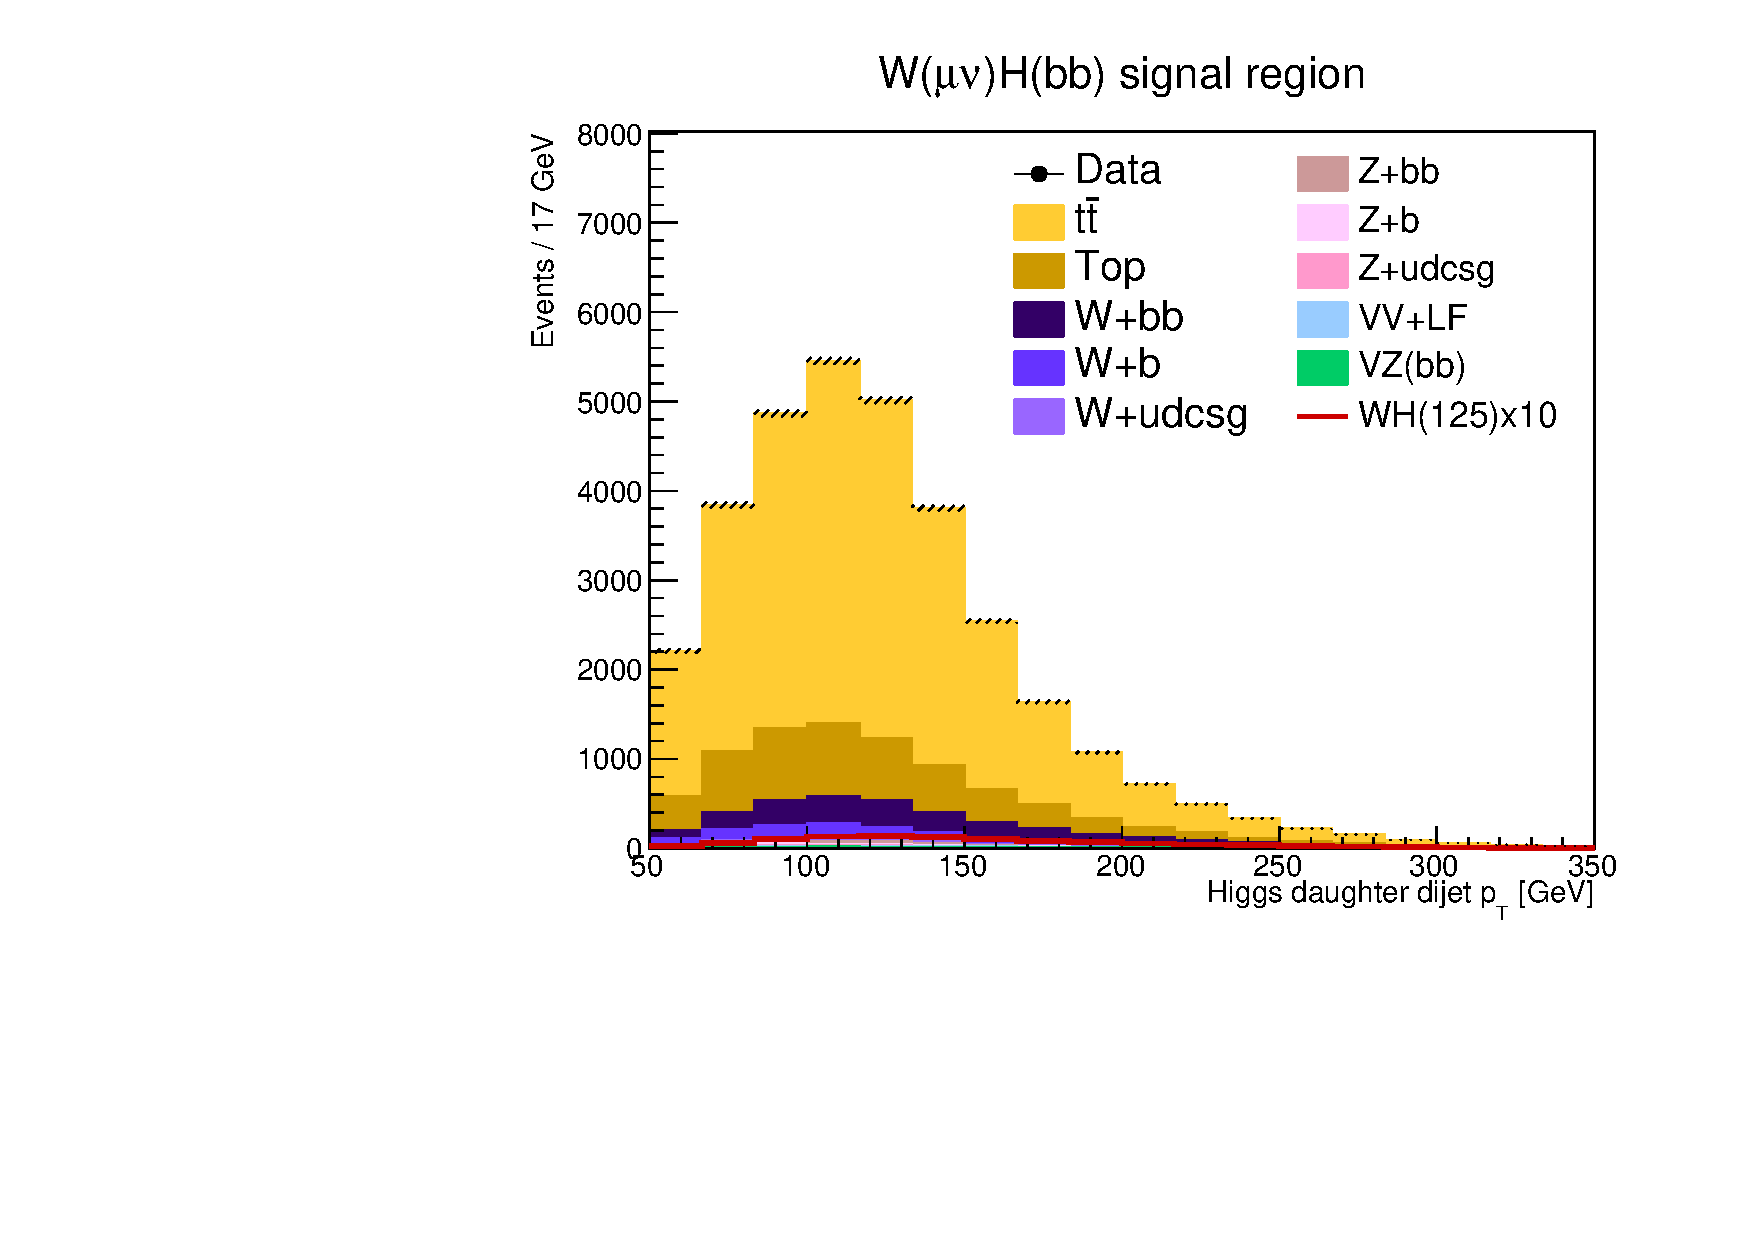
\includegraphics[width=0.48\textwidth]{figures/wlnhbb2016/resolved/WmnWHSR_pTH.pdf}
    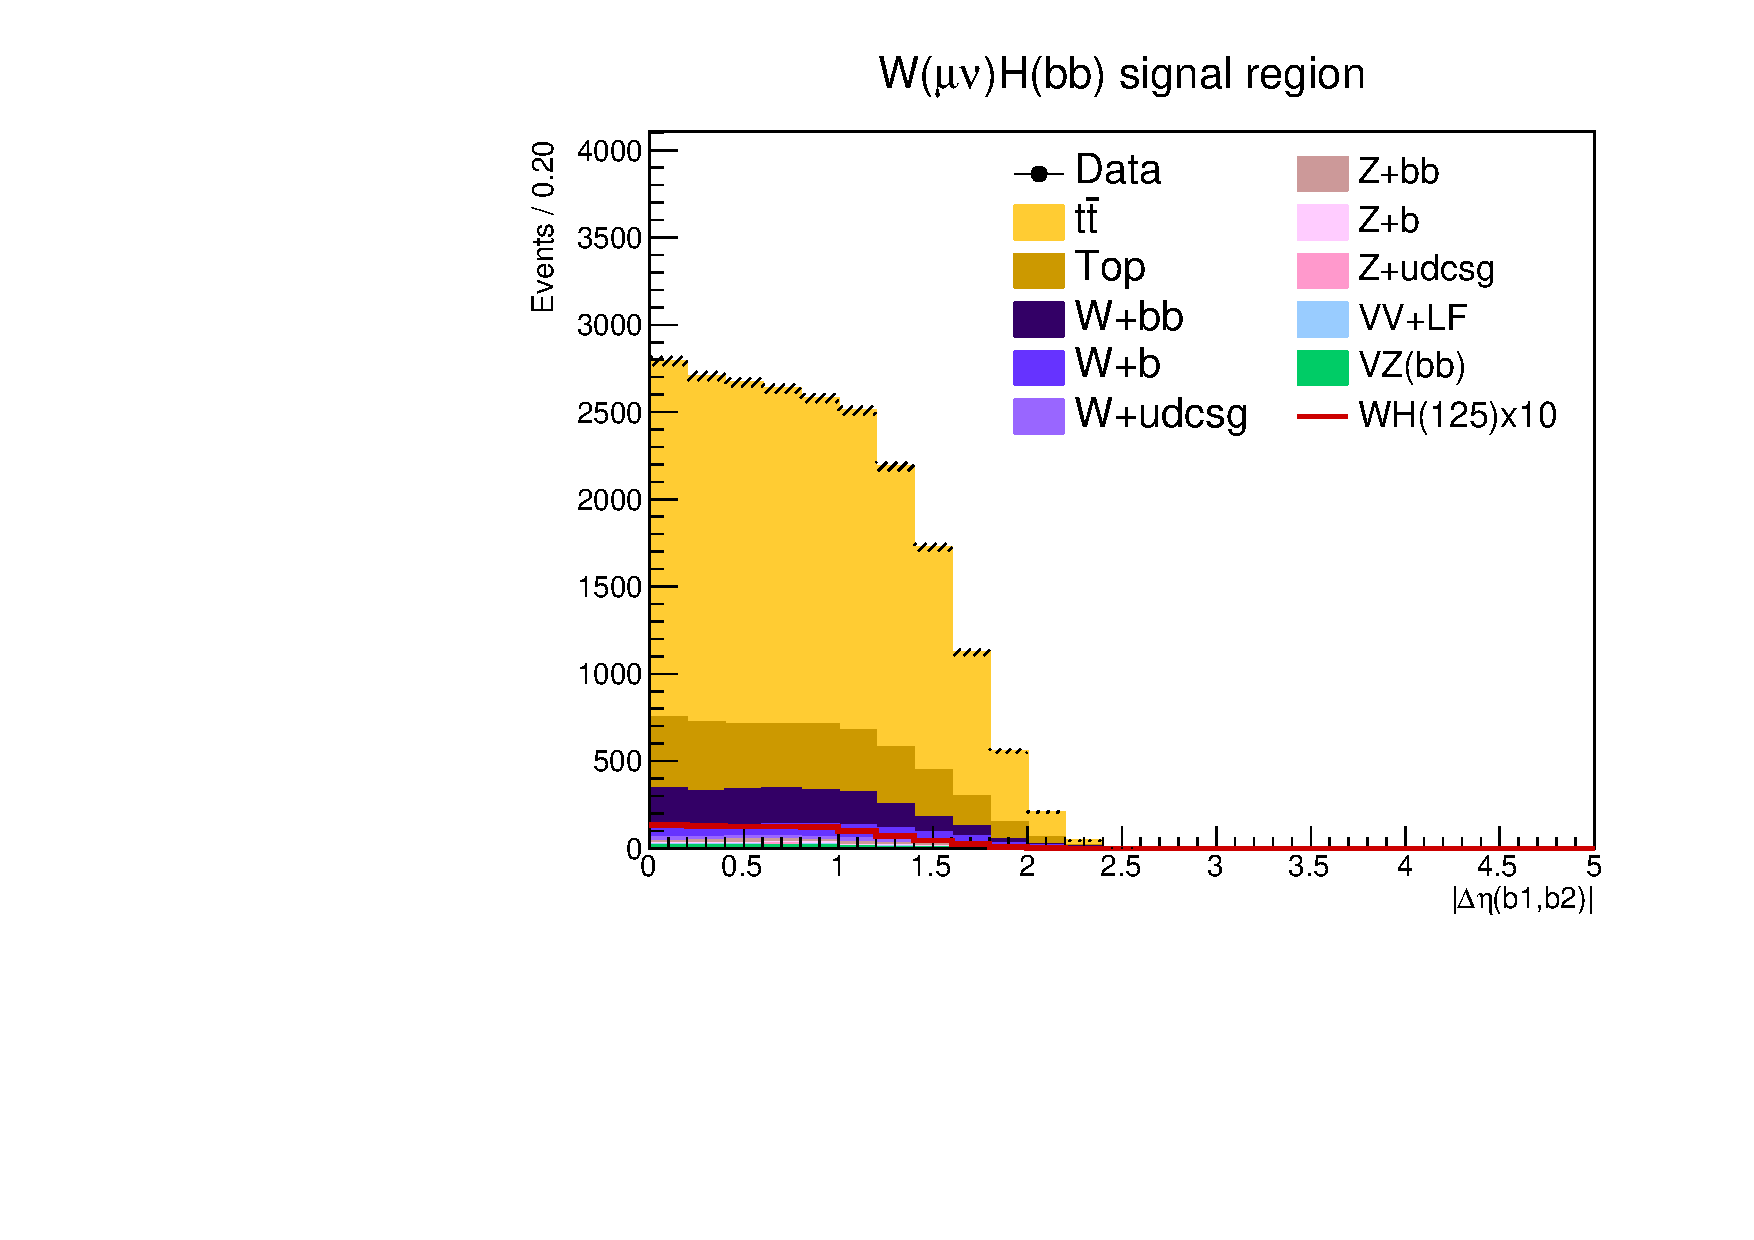
\includegraphics[width=0.48\textwidth]{figures/wlnhbb2016/resolved/WmnWHSR_dEtab1b2.pdf}
    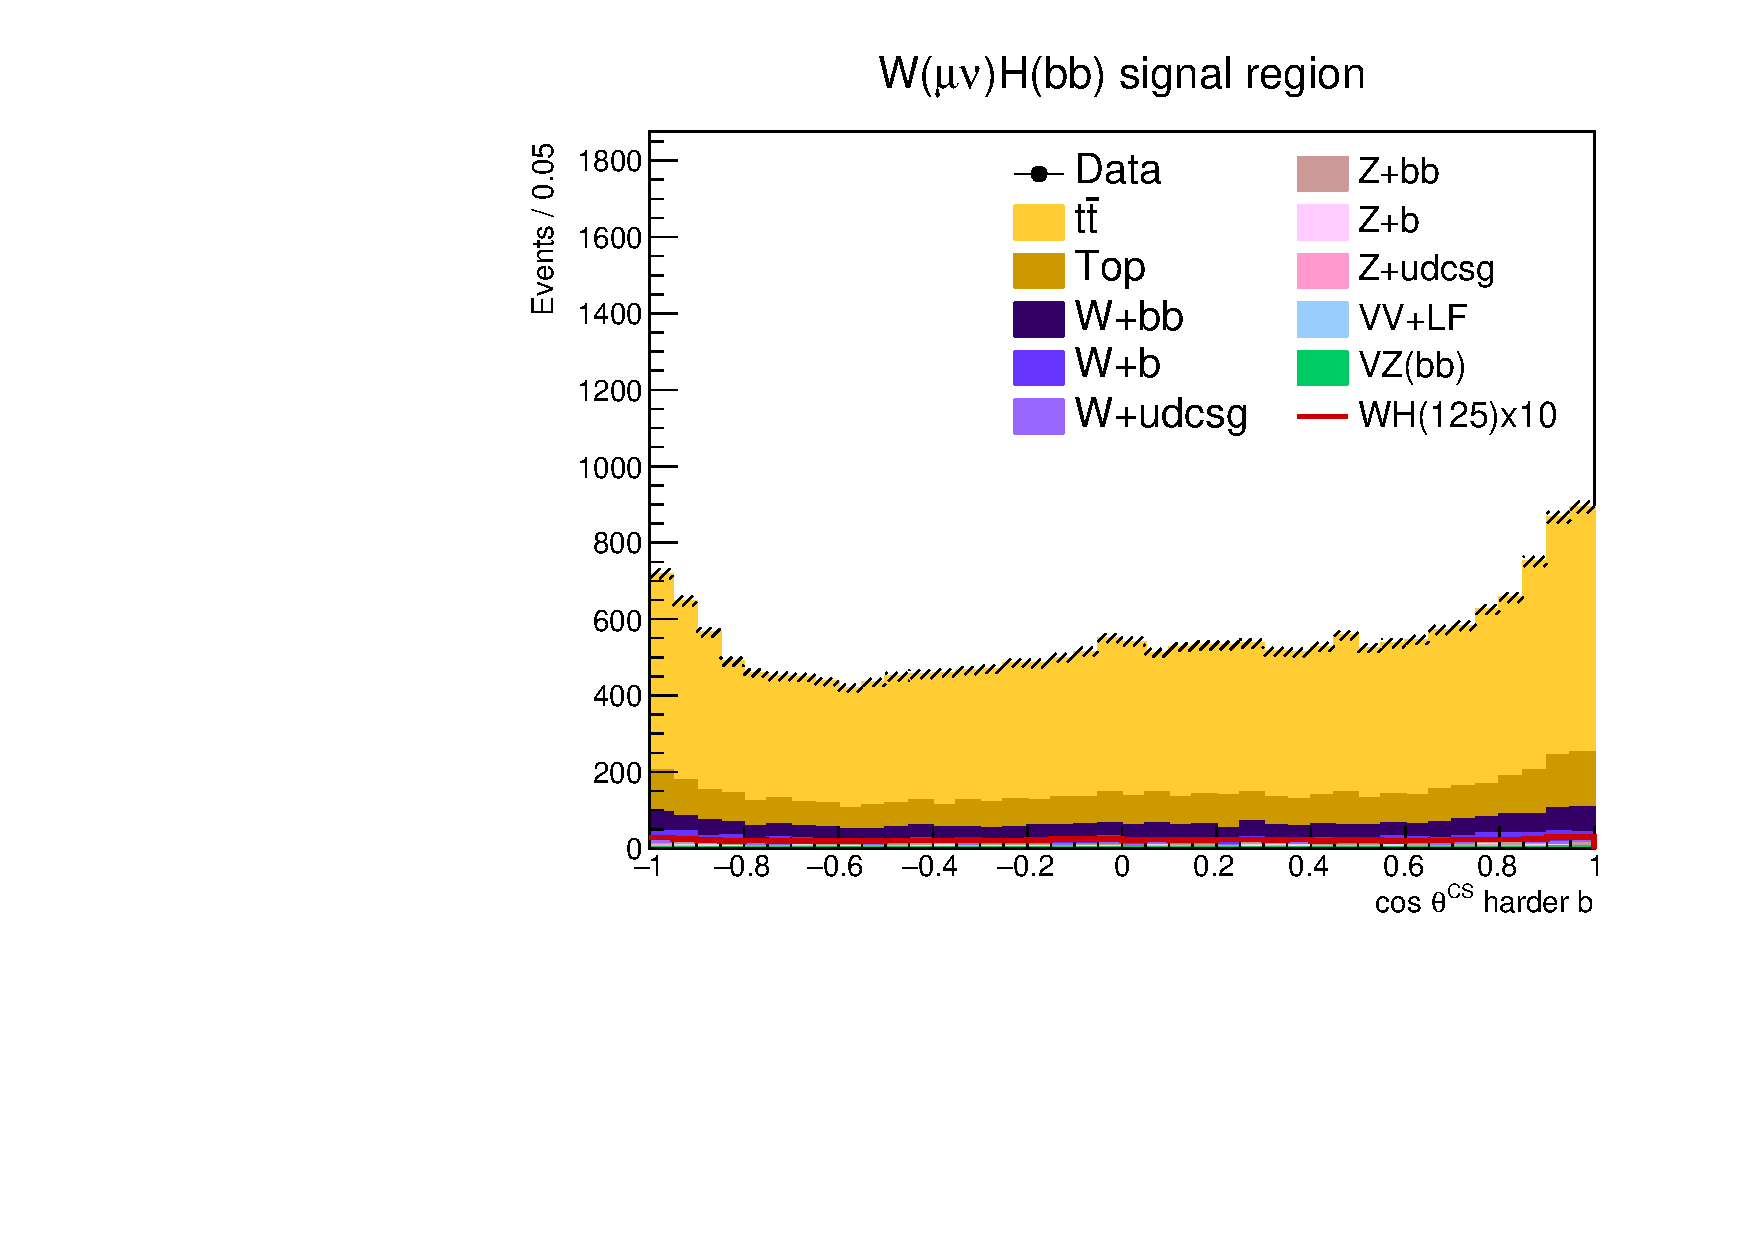
\includegraphics[width=0.48\textwidth]{figures/wlnhbb2016/resolved/WmnWHSR_hbbCosThetaCSJ1.pdf}
    \caption{\HBB\ reconstruction in the resolved category W($\mu\nu$) signal region.
    Left to right and top to bottom: higher b-tagged jet $\pt$, lower b-tagged jet $\pt$, dijet mass, dijet $\pt$, 
    pseudorapidity difference between the two jets, and the Collins-Soper angle of the harder b-tagged jet.
    The simulated shapes are prefit, with the postfit normalizations applied.}
    \label{fig:res_WmnSR_Hbb}
  \end{center}
\end{figure}
\clearpage

\begin{figure}[tbp]
  \begin{center}
    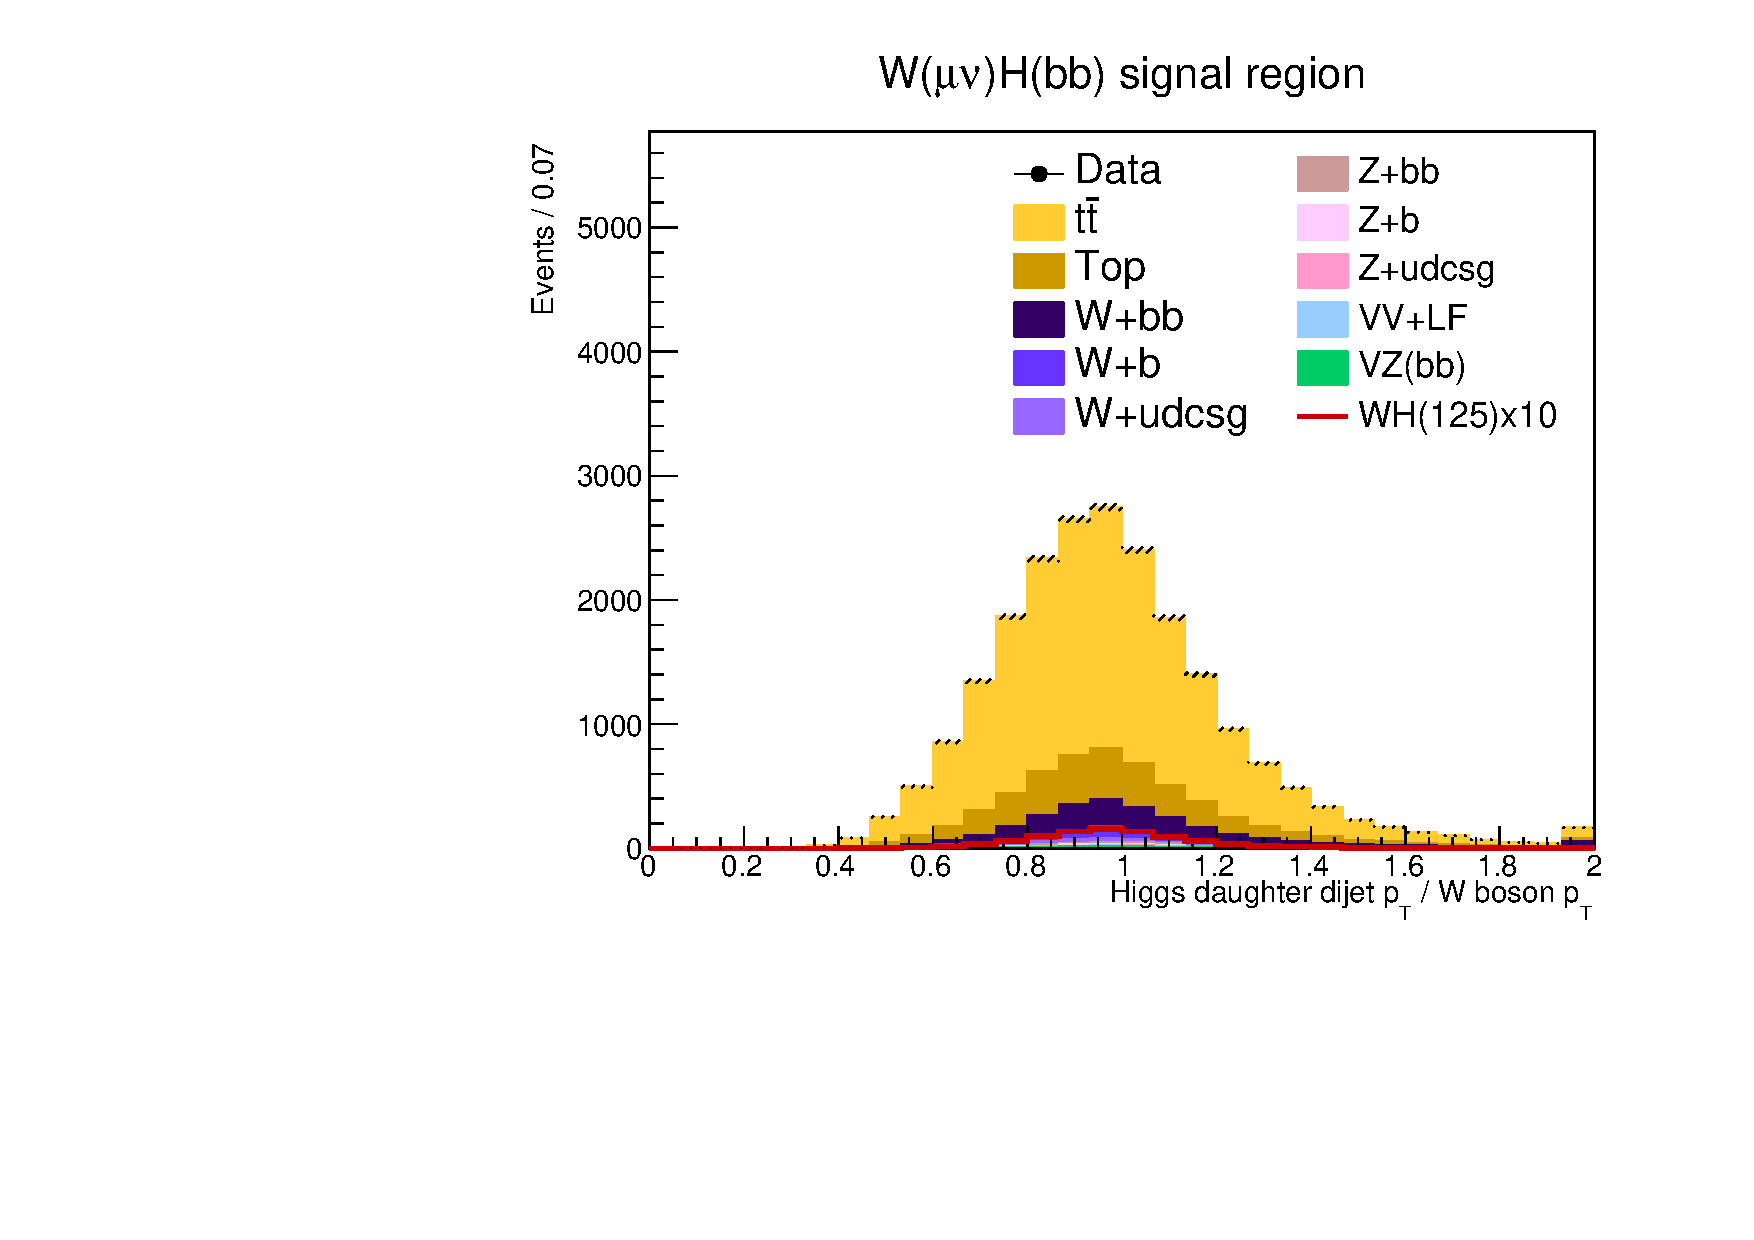
\includegraphics[width=0.48\textwidth]{figures/wlnhbb2016/resolved/WmnWHSR_pTBalanceDijetW.pdf}
    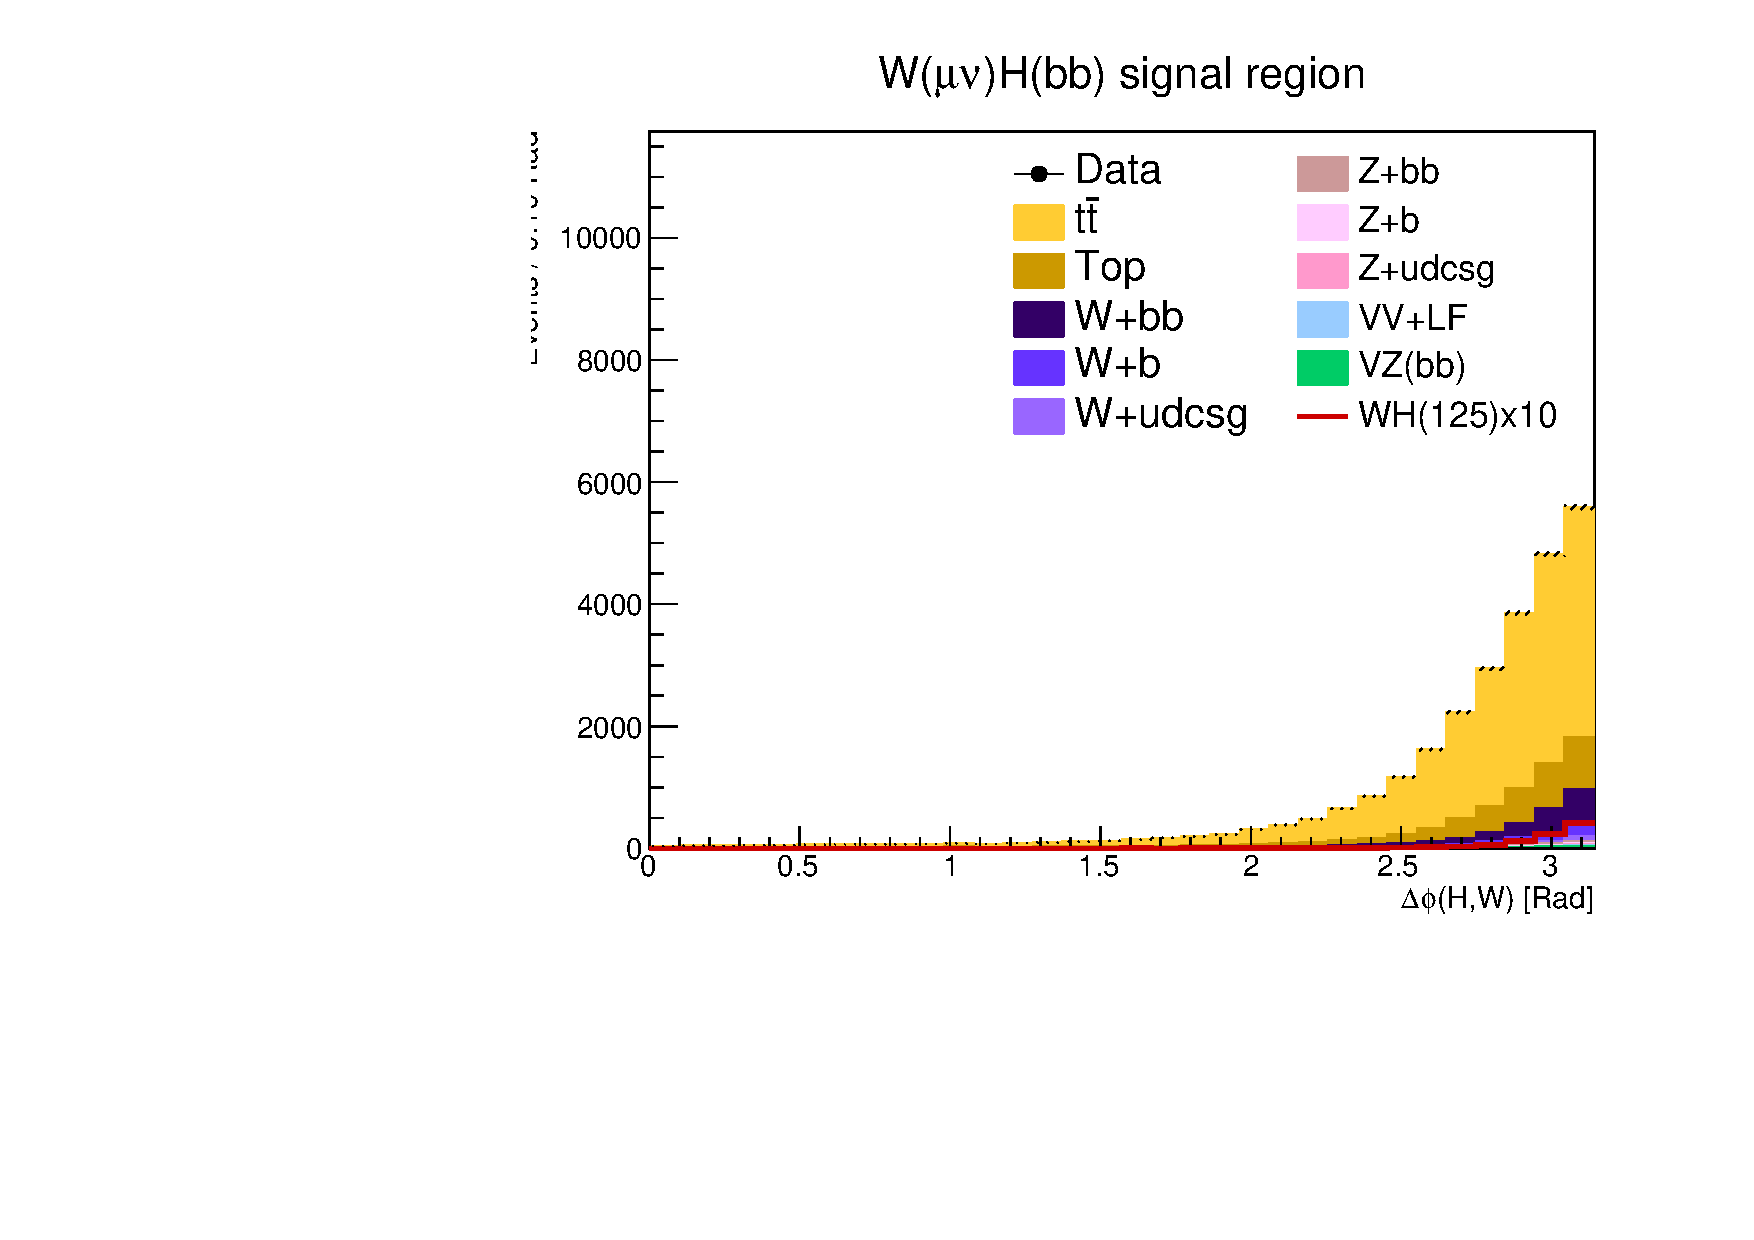
\includegraphics[width=0.48\textwidth]{figures/wlnhbb2016/resolved/WmnWHSR_deltaPhiVH.pdf}
    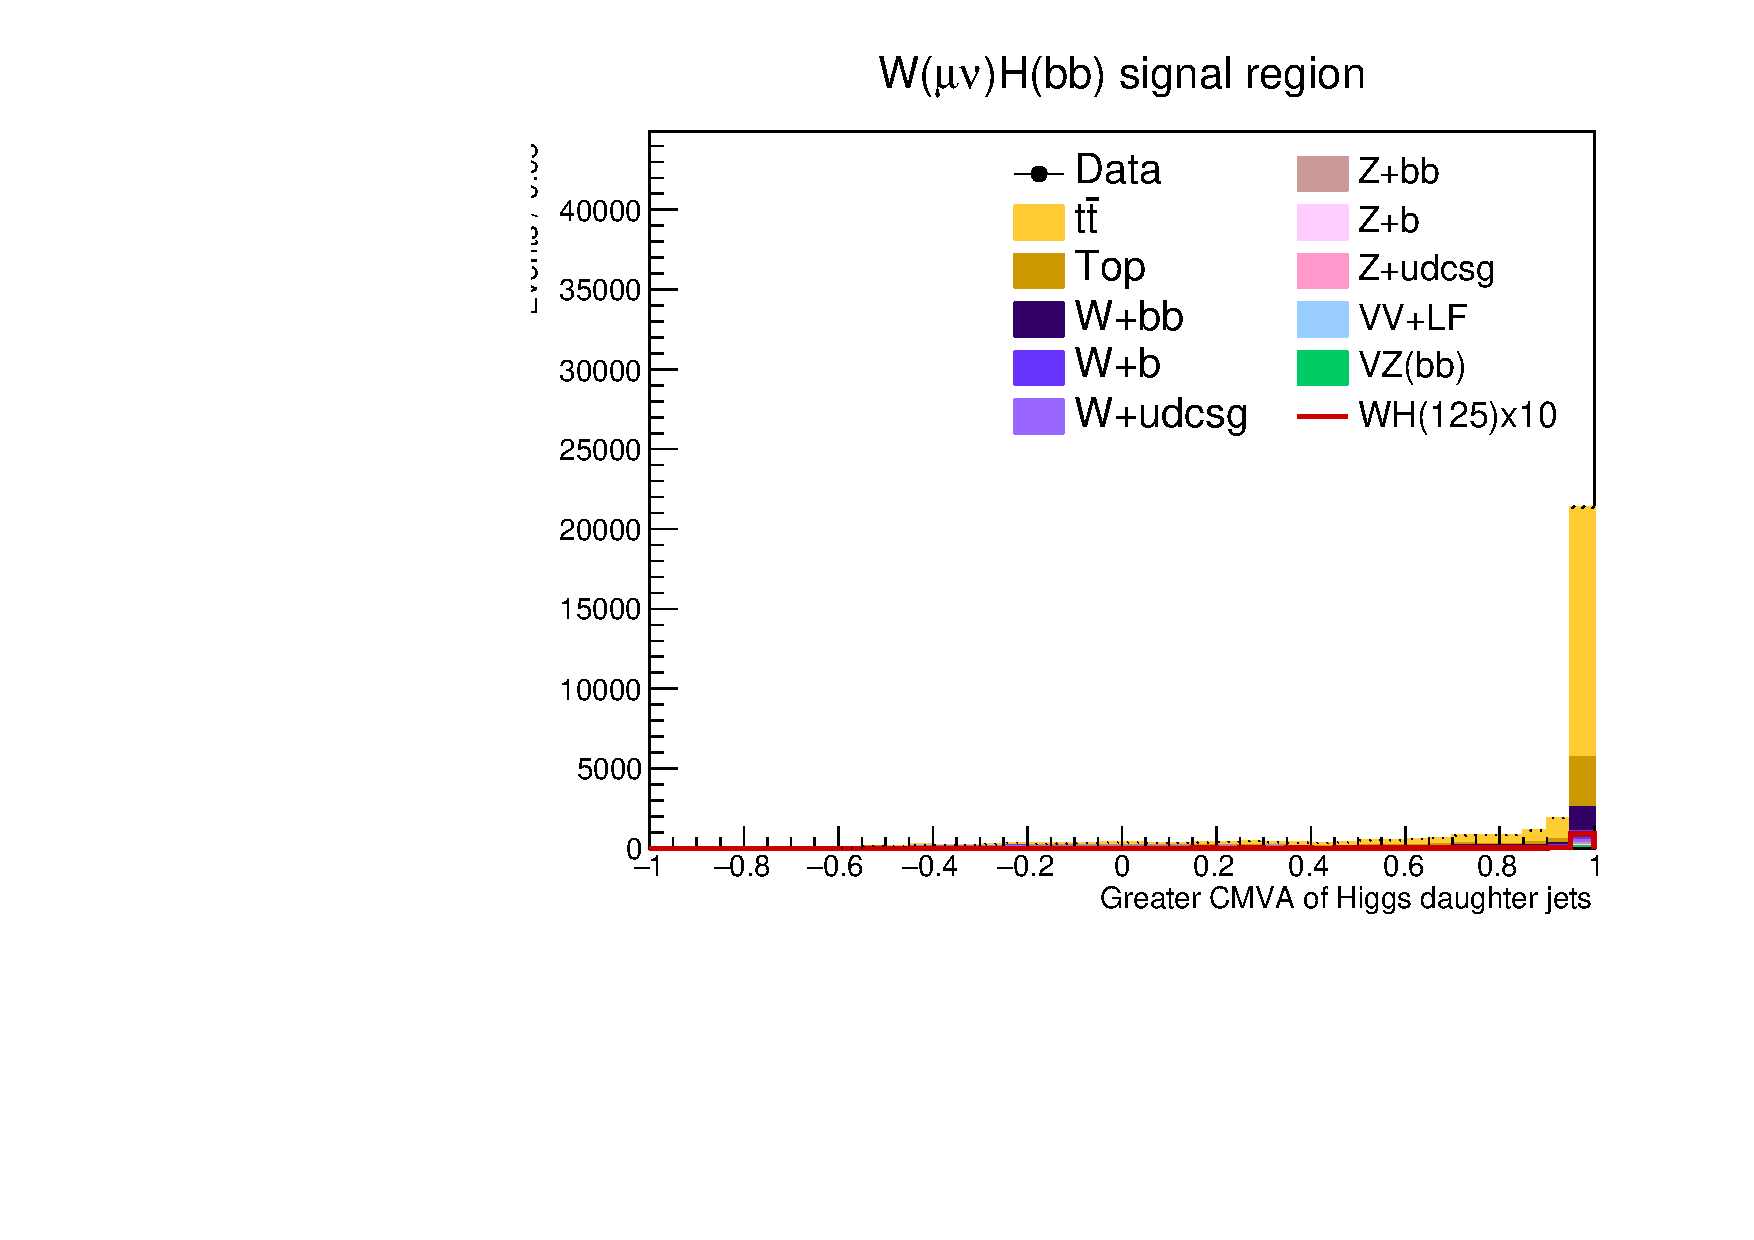
\includegraphics[width=0.48\textwidth]{figures/wlnhbb2016/resolved/WmnWHSR_bDiscrMax.pdf}
    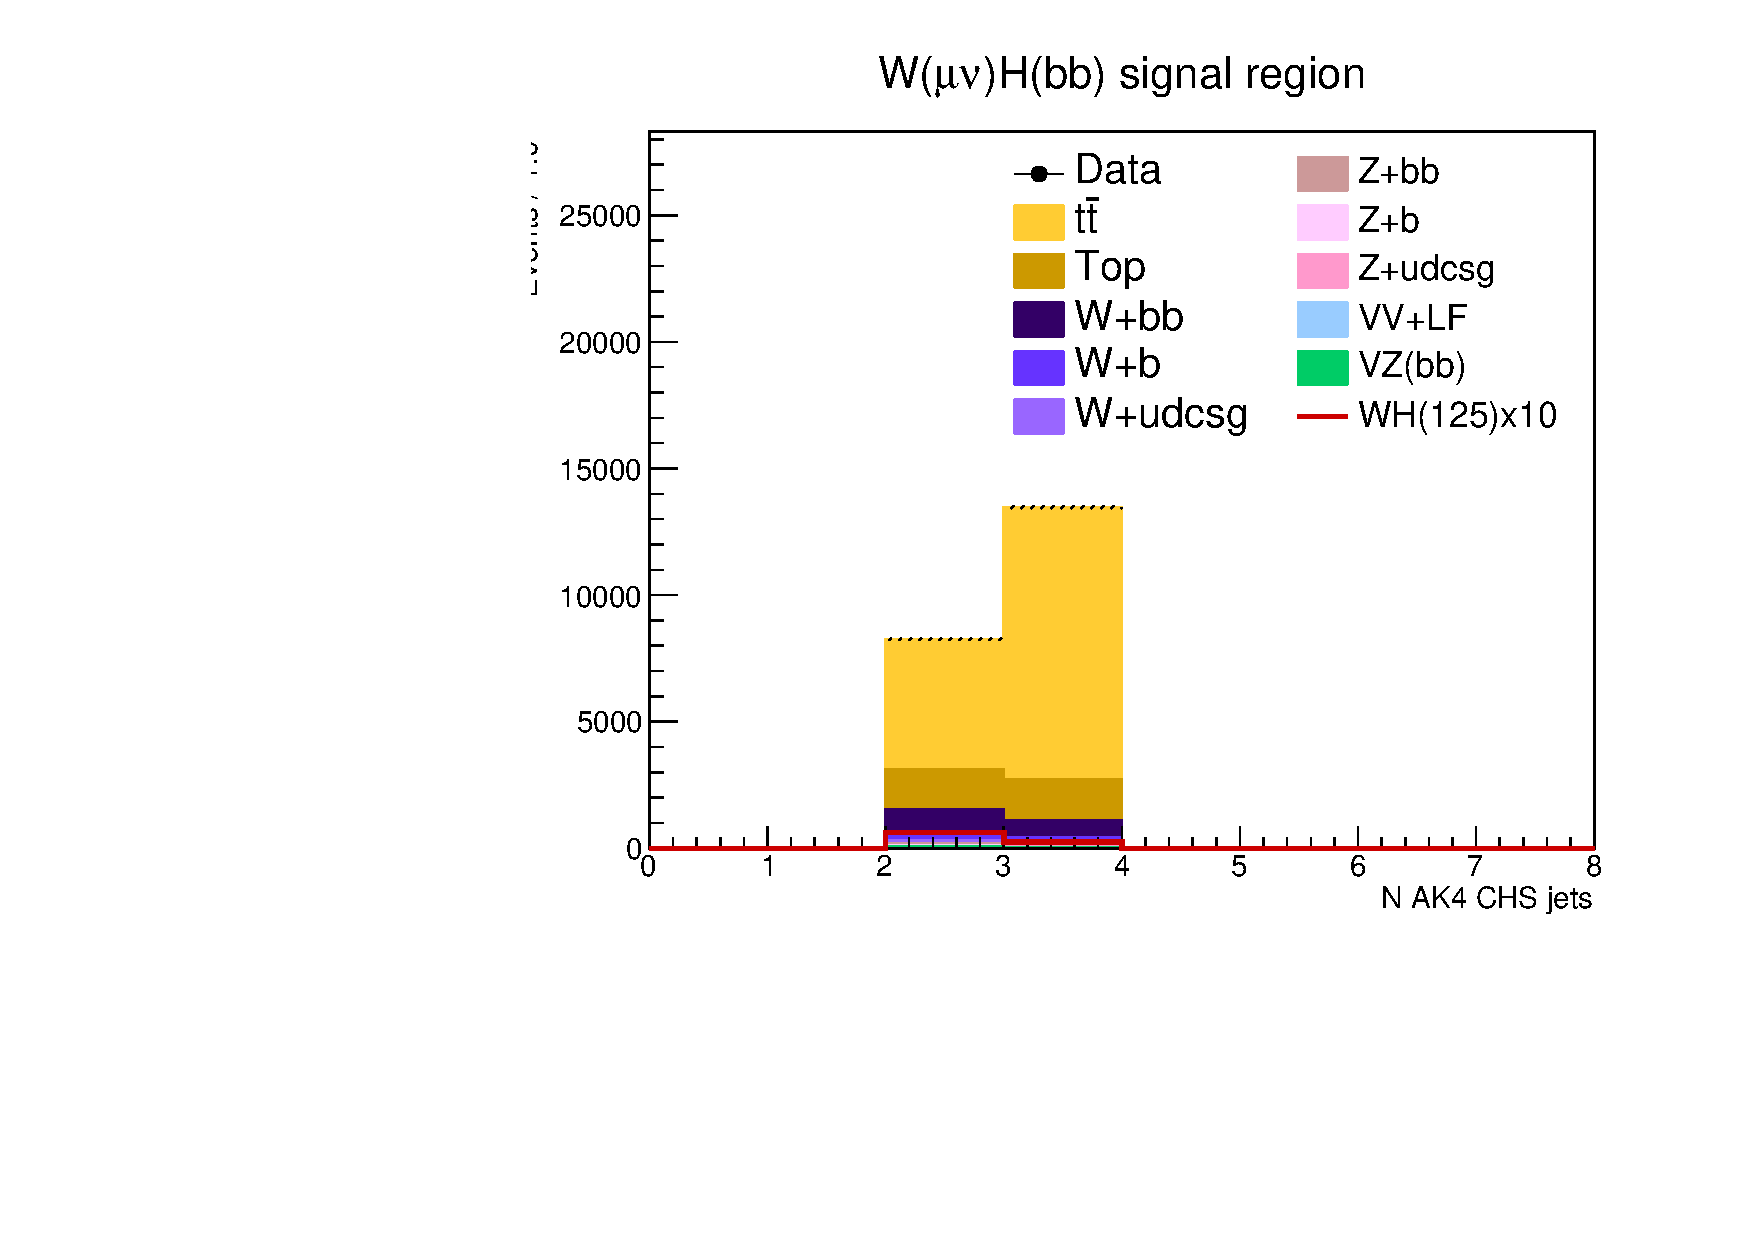
\includegraphics[width=0.48\textwidth]{figures/wlnhbb2016/resolved/WmnWHSR_nJet.pdf}
    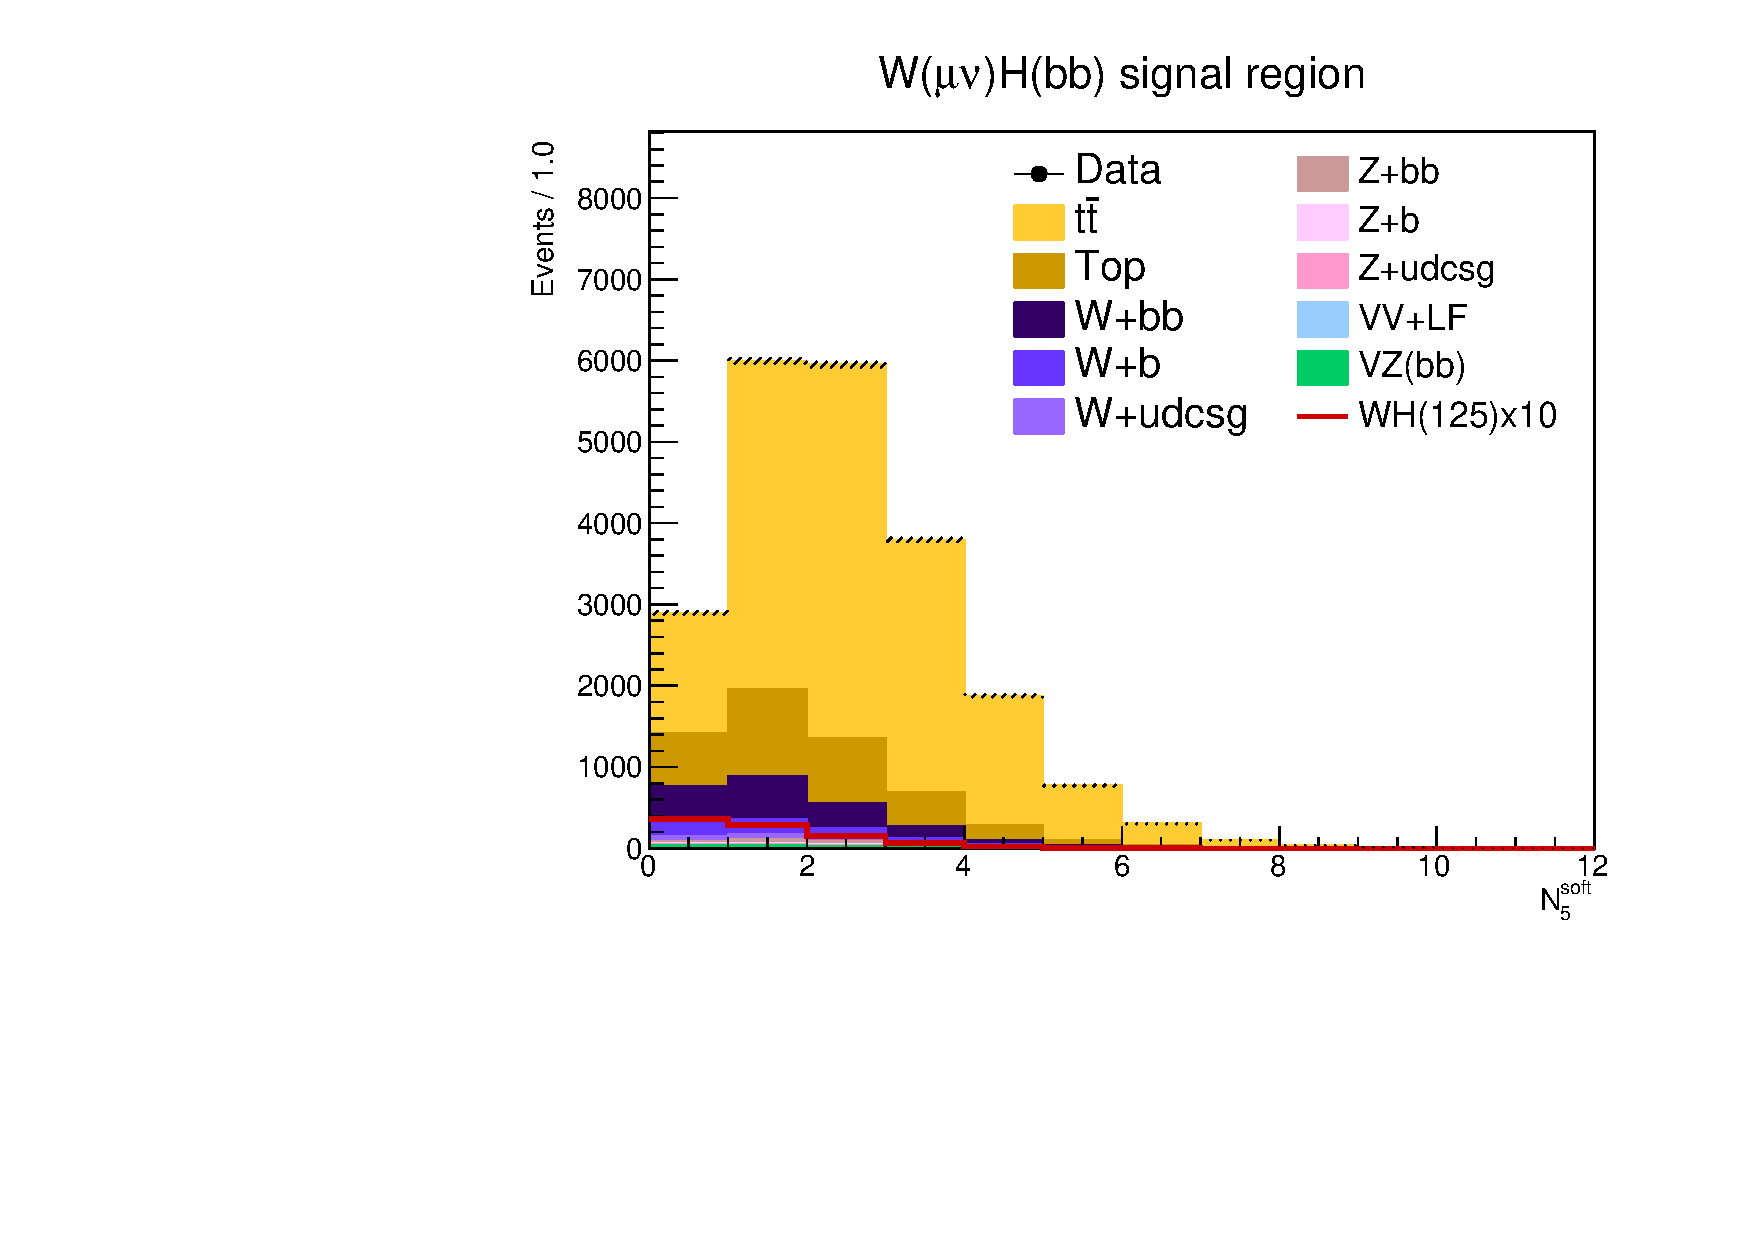
\includegraphics[width=0.48\textwidth]{figures/wlnhbb2016/resolved/WmnWHSR_nSoft5.pdf}
    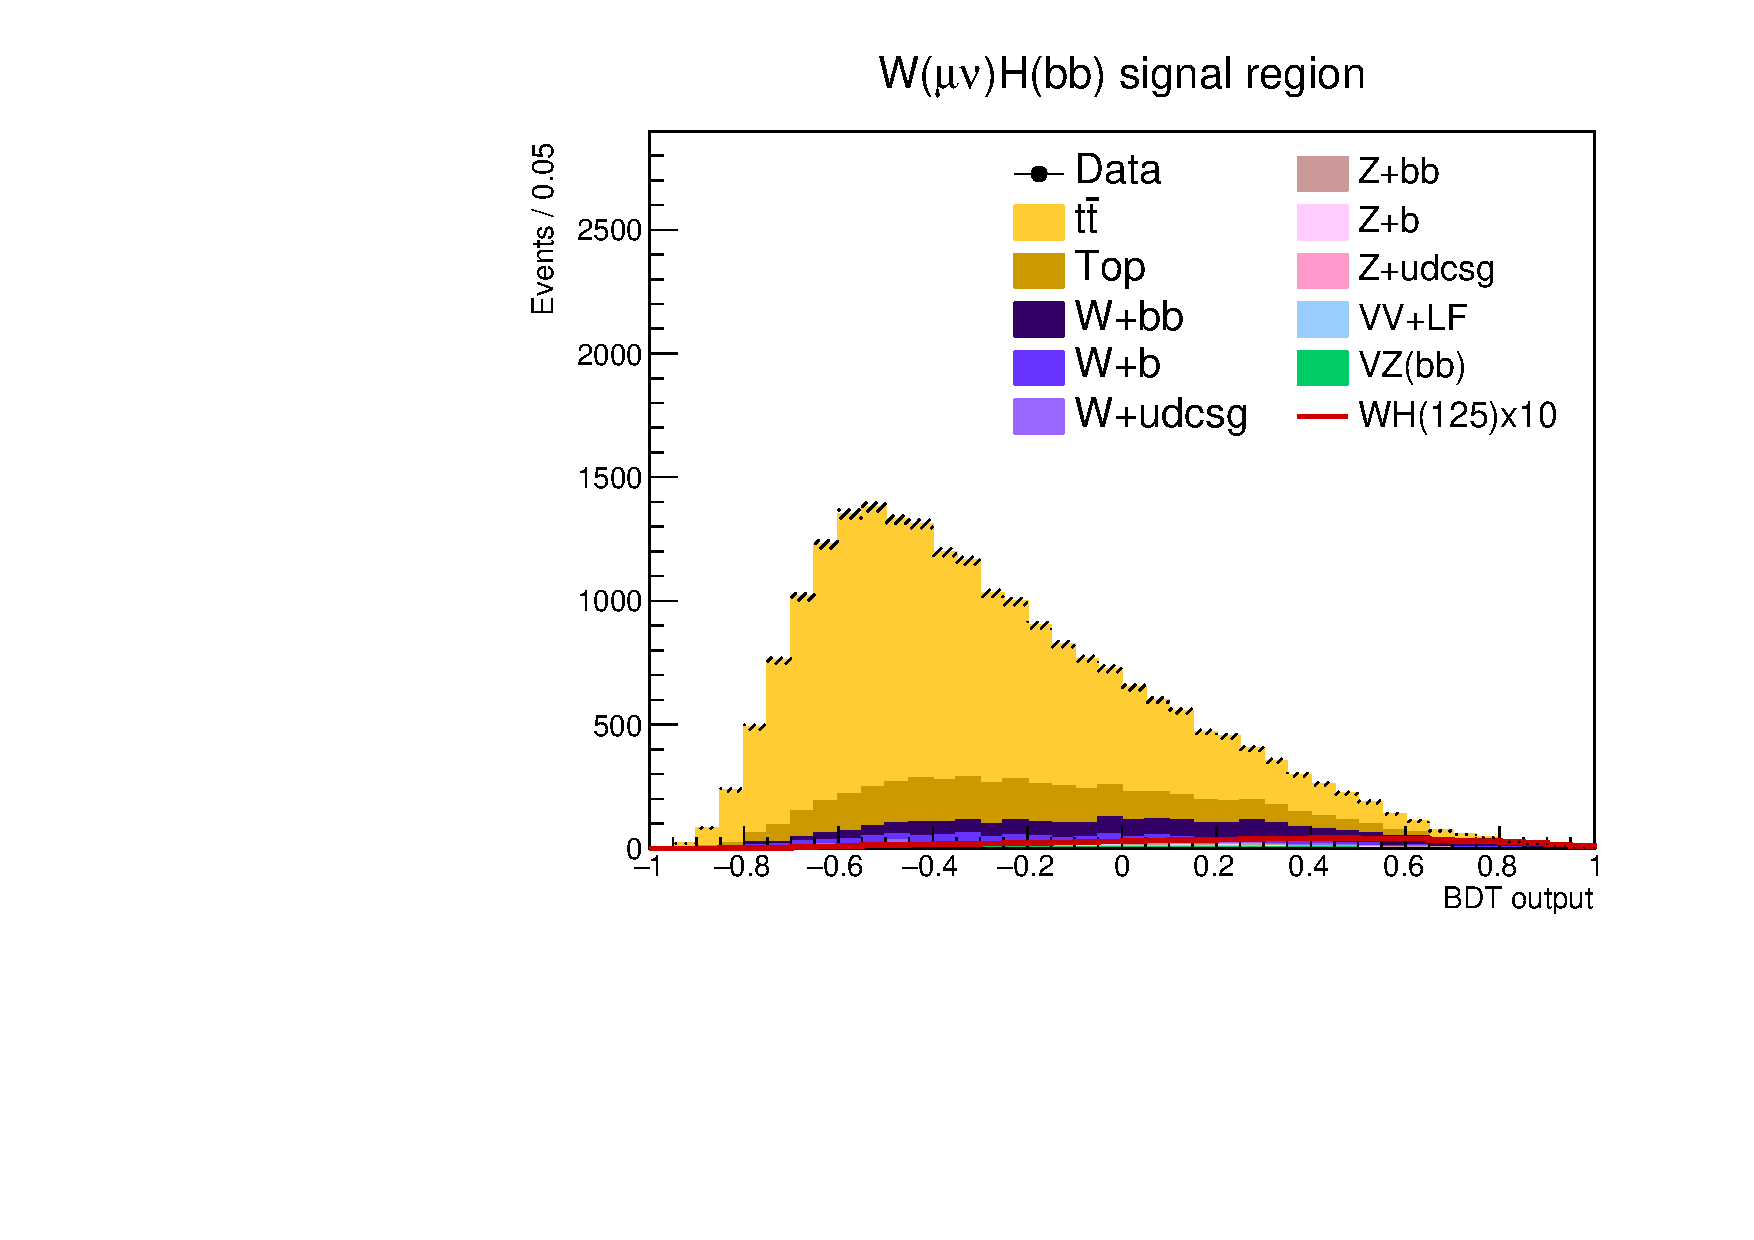
\includegraphics[width=0.48\textwidth]{figures/wlnhbb2016/resolved/WmnWHSR_bdtValue.pdf}
    \caption{WH kinematics in the resolved category W($\mu\nu$) signal region.
    Left to right and top to bottom: WH $\pt$ balance, WH azimuthal separation, leading b-tag score, the number of central jets,
    the number of 5 \GeV\ soft activity jets, and the evaluation of the signal extraction BDT.
    The simulated shapes are prefit, with the postfit normalizations applied.}
    \label{fig:res_WmnSR_WH}
  \end{center}
\end{figure}
\clearpage

\begin{figure}[tbp]
  \begin{center}
    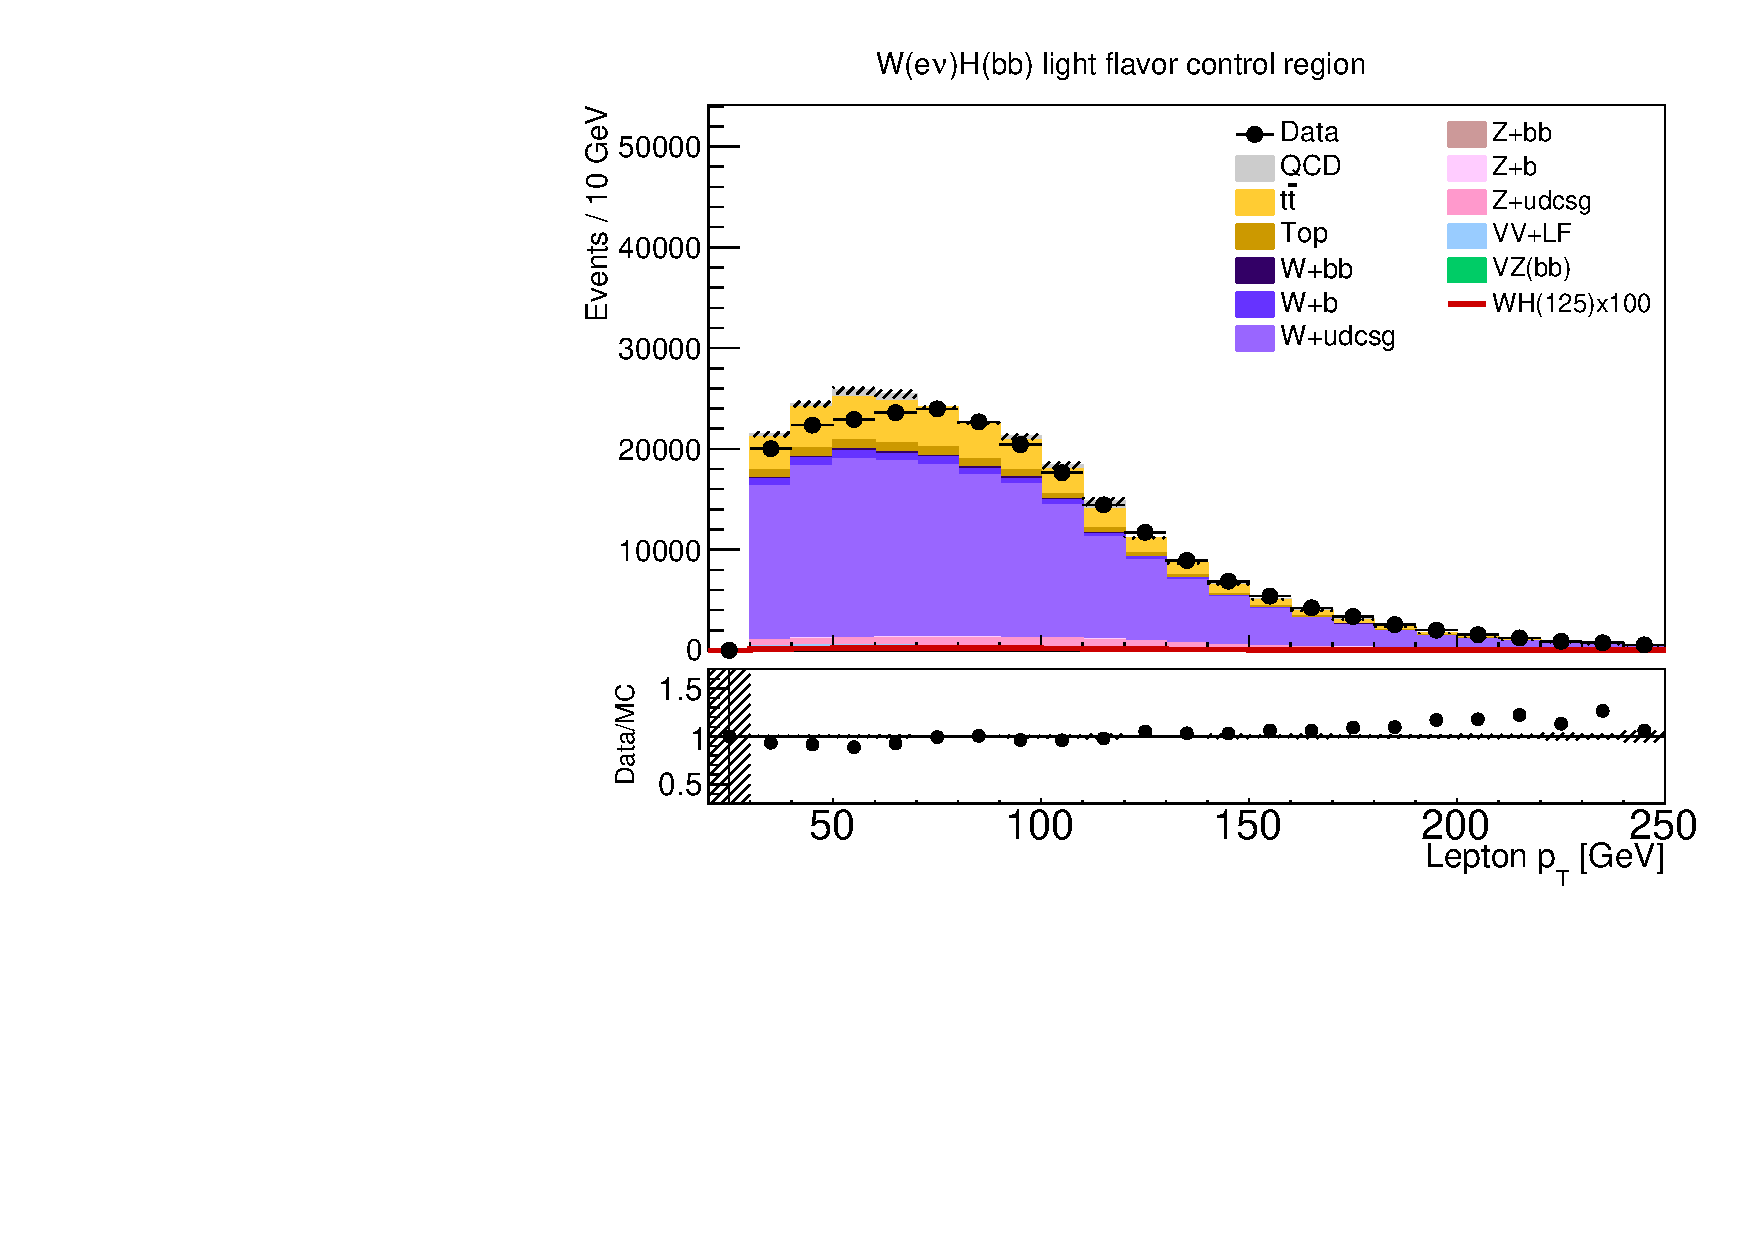
\includegraphics[width=0.48\textwidth]{figures/wlnhbb2016/resolved/WenWHLightFlavorCR_lepton1Pt.pdf}
    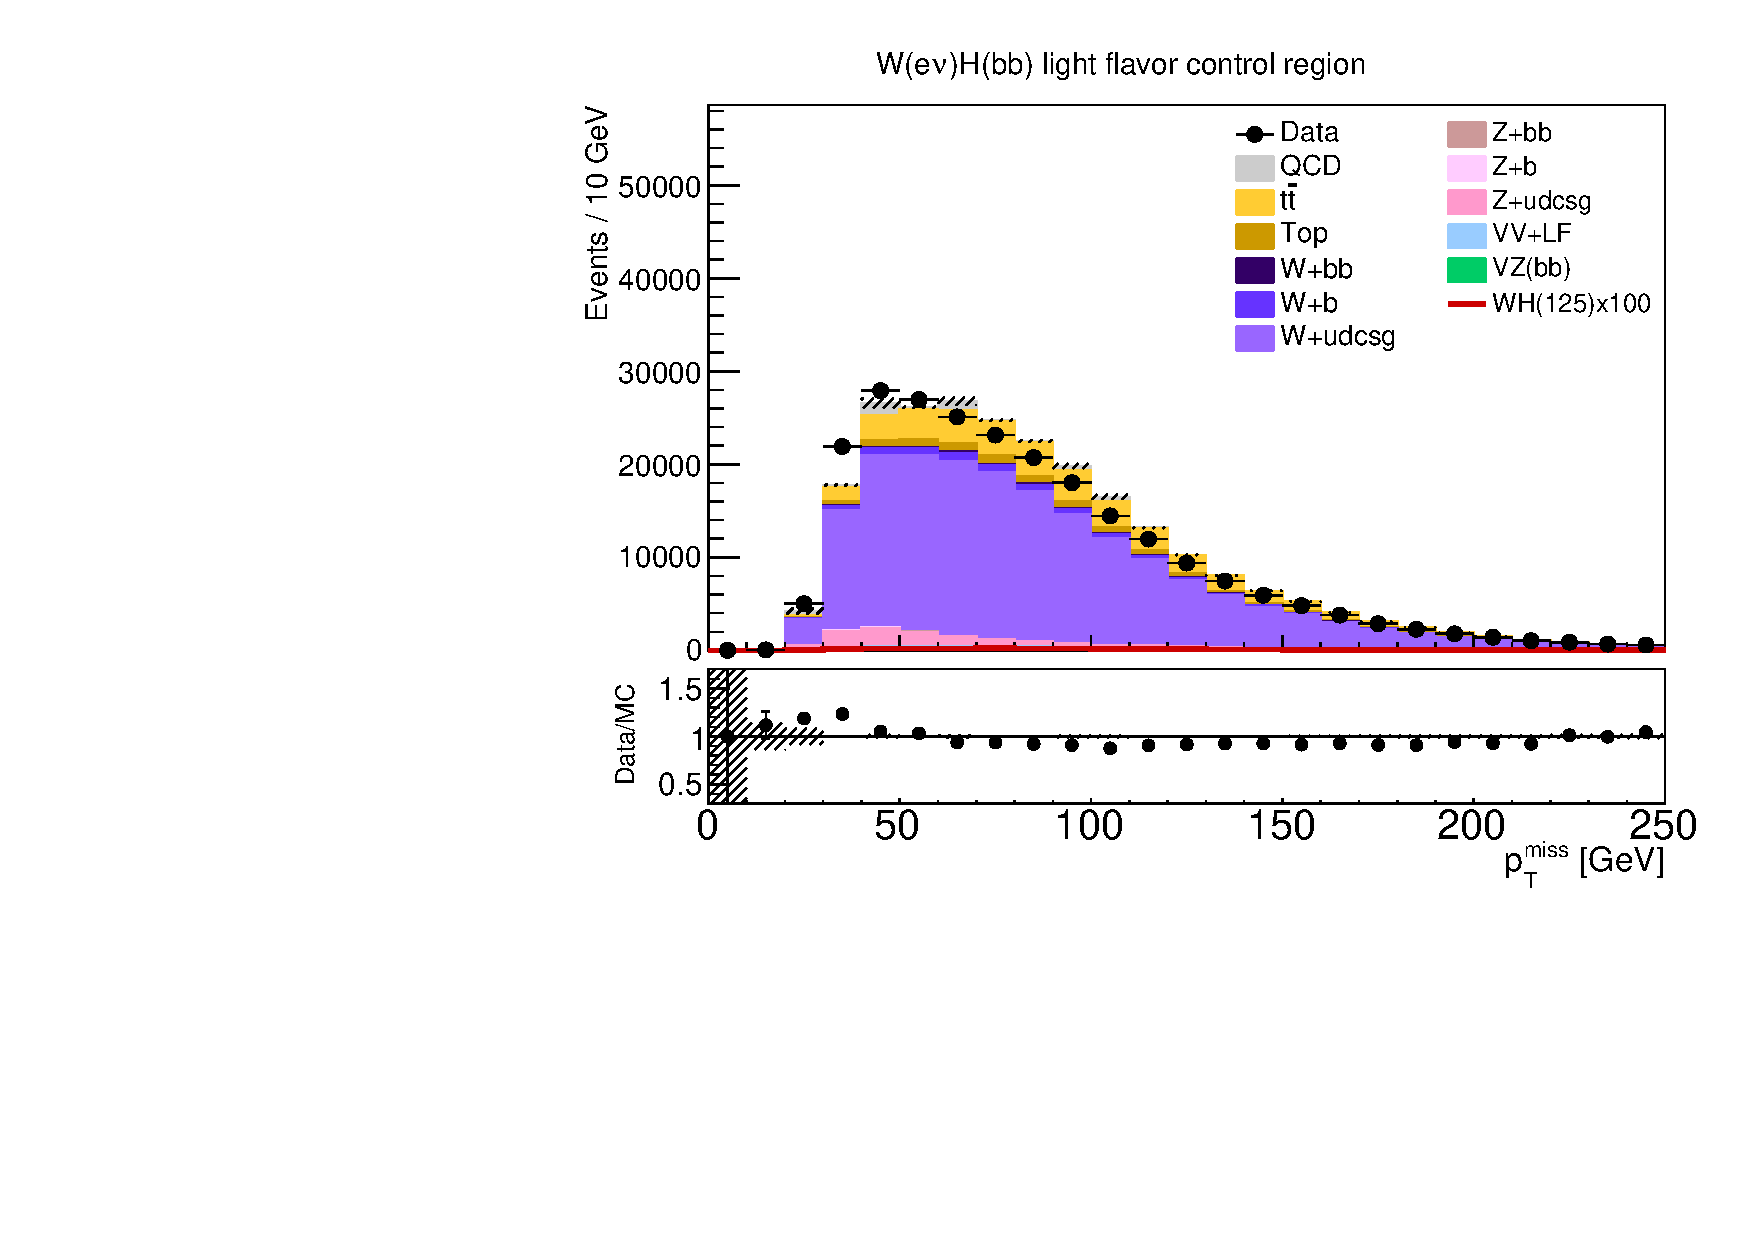
\includegraphics[width=0.48\textwidth]{figures/wlnhbb2016/resolved/WenWHLightFlavorCR_pfmet.pdf}
    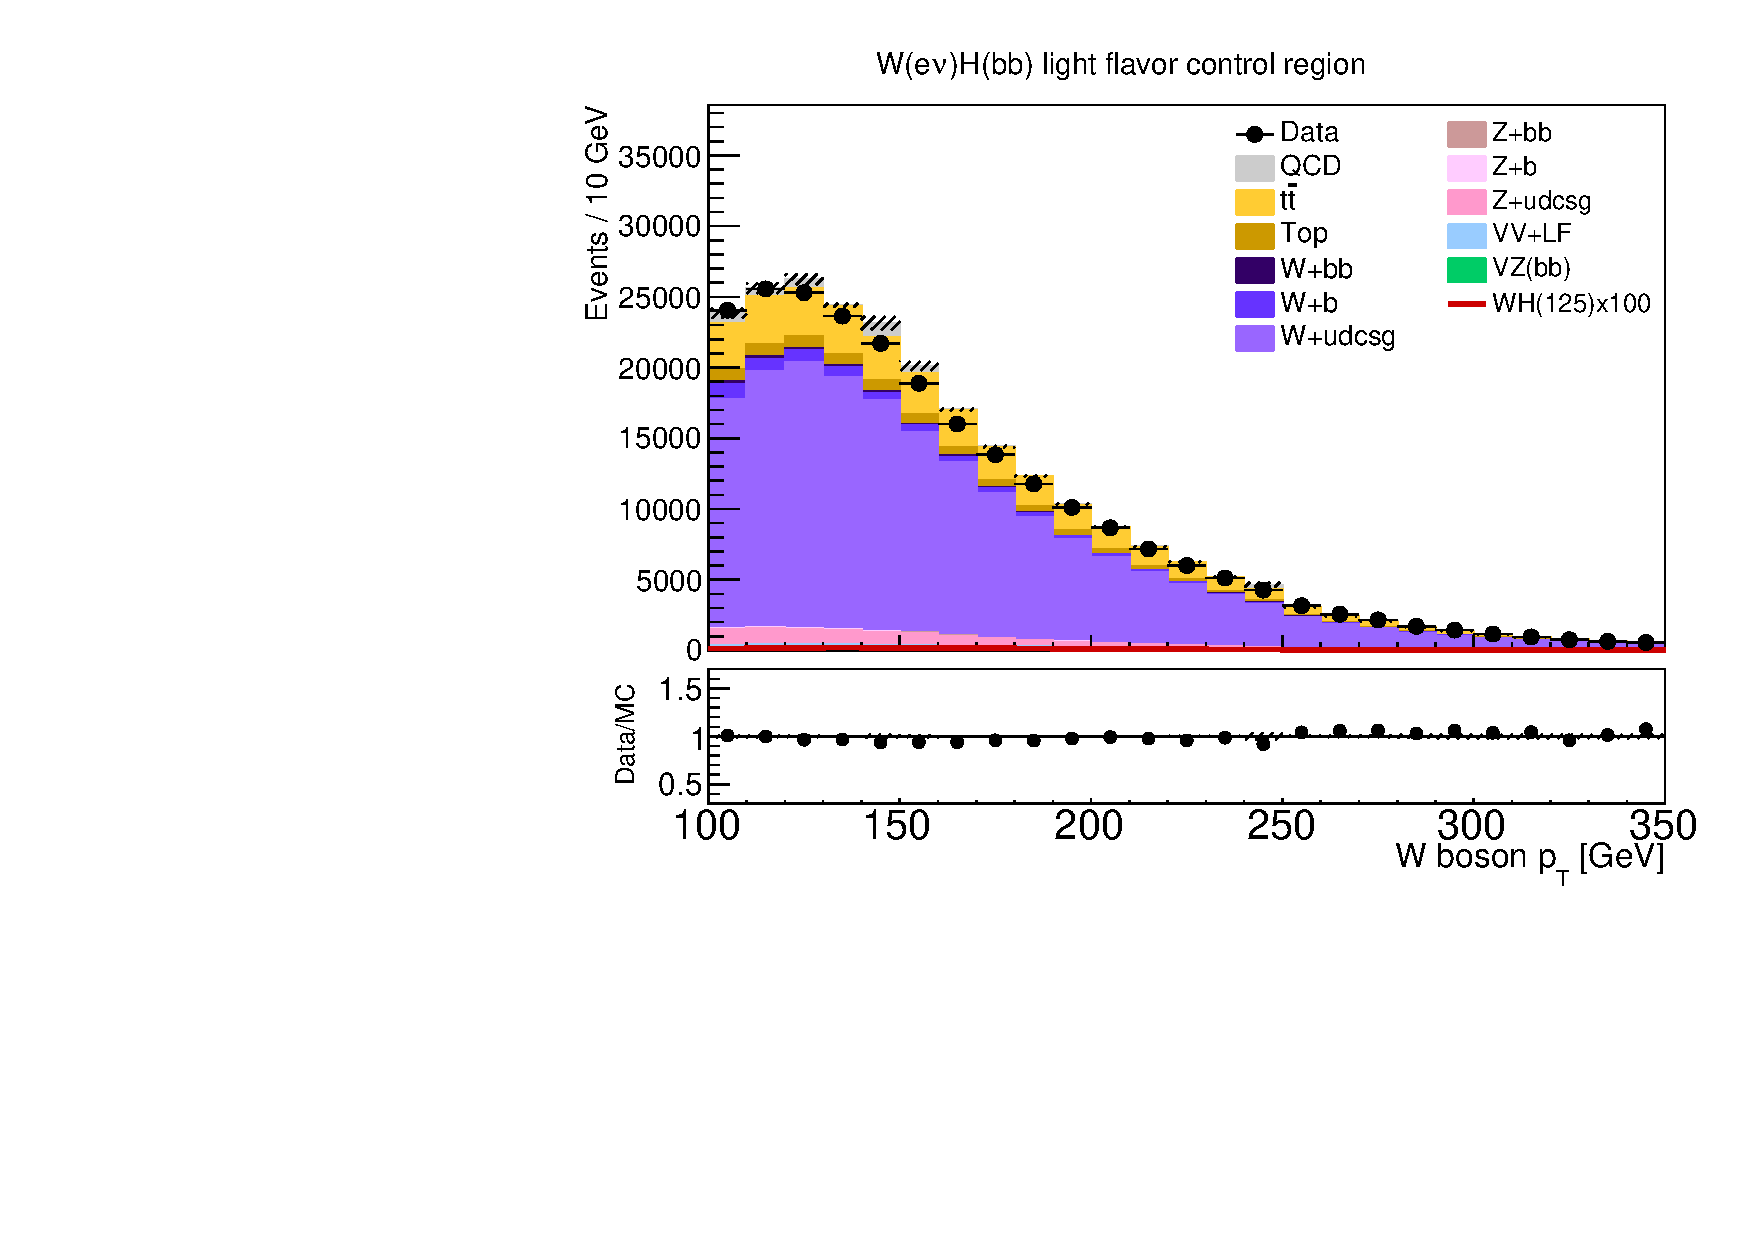
\includegraphics[width=0.48\textwidth]{figures/wlnhbb2016/resolved/WenWHLightFlavorCR_WpT.pdf}
    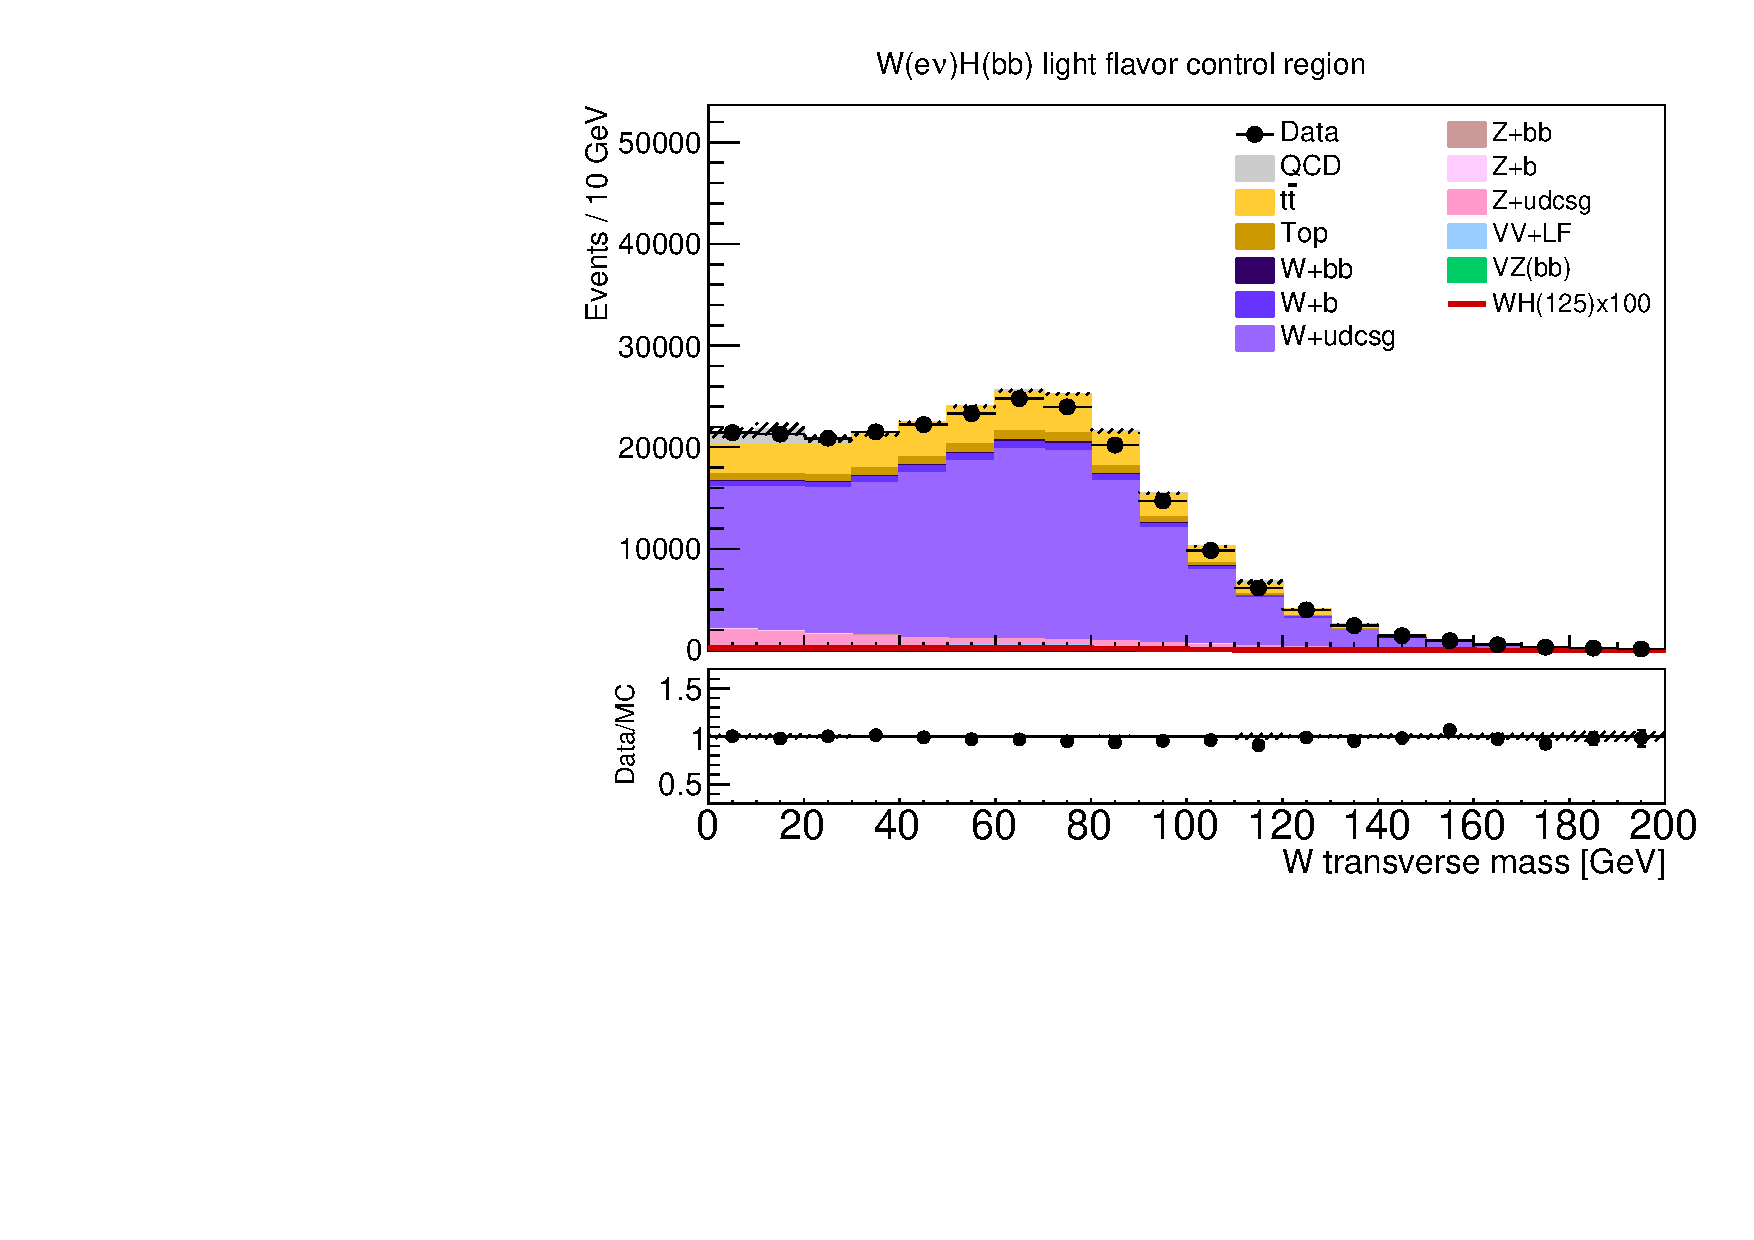
\includegraphics[width=0.48\textwidth]{figures/wlnhbb2016/resolved/WenWHLightFlavorCR_mTW.pdf}
    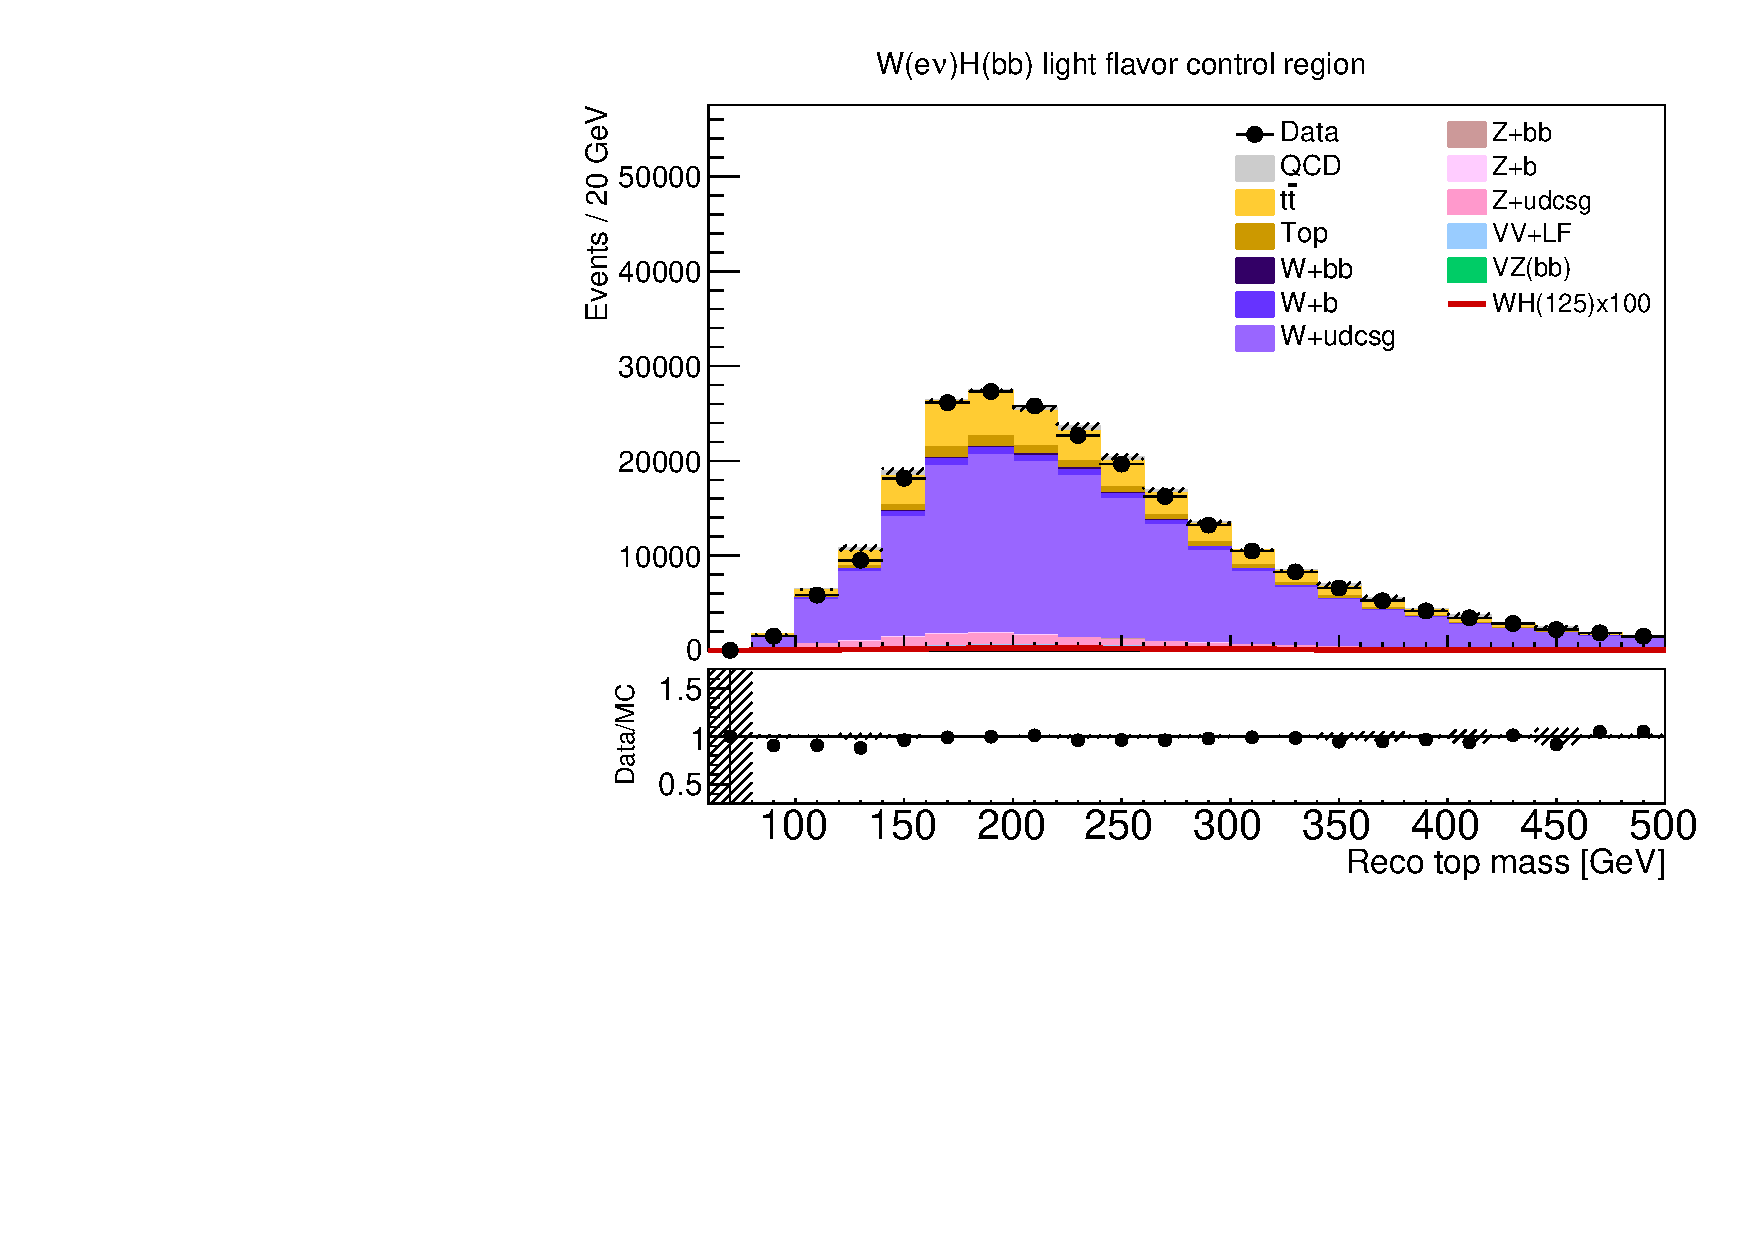
\includegraphics[width=0.48\textwidth]{figures/wlnhbb2016/resolved/WenWHLightFlavorCR_topMassLep1Met.pdf}
    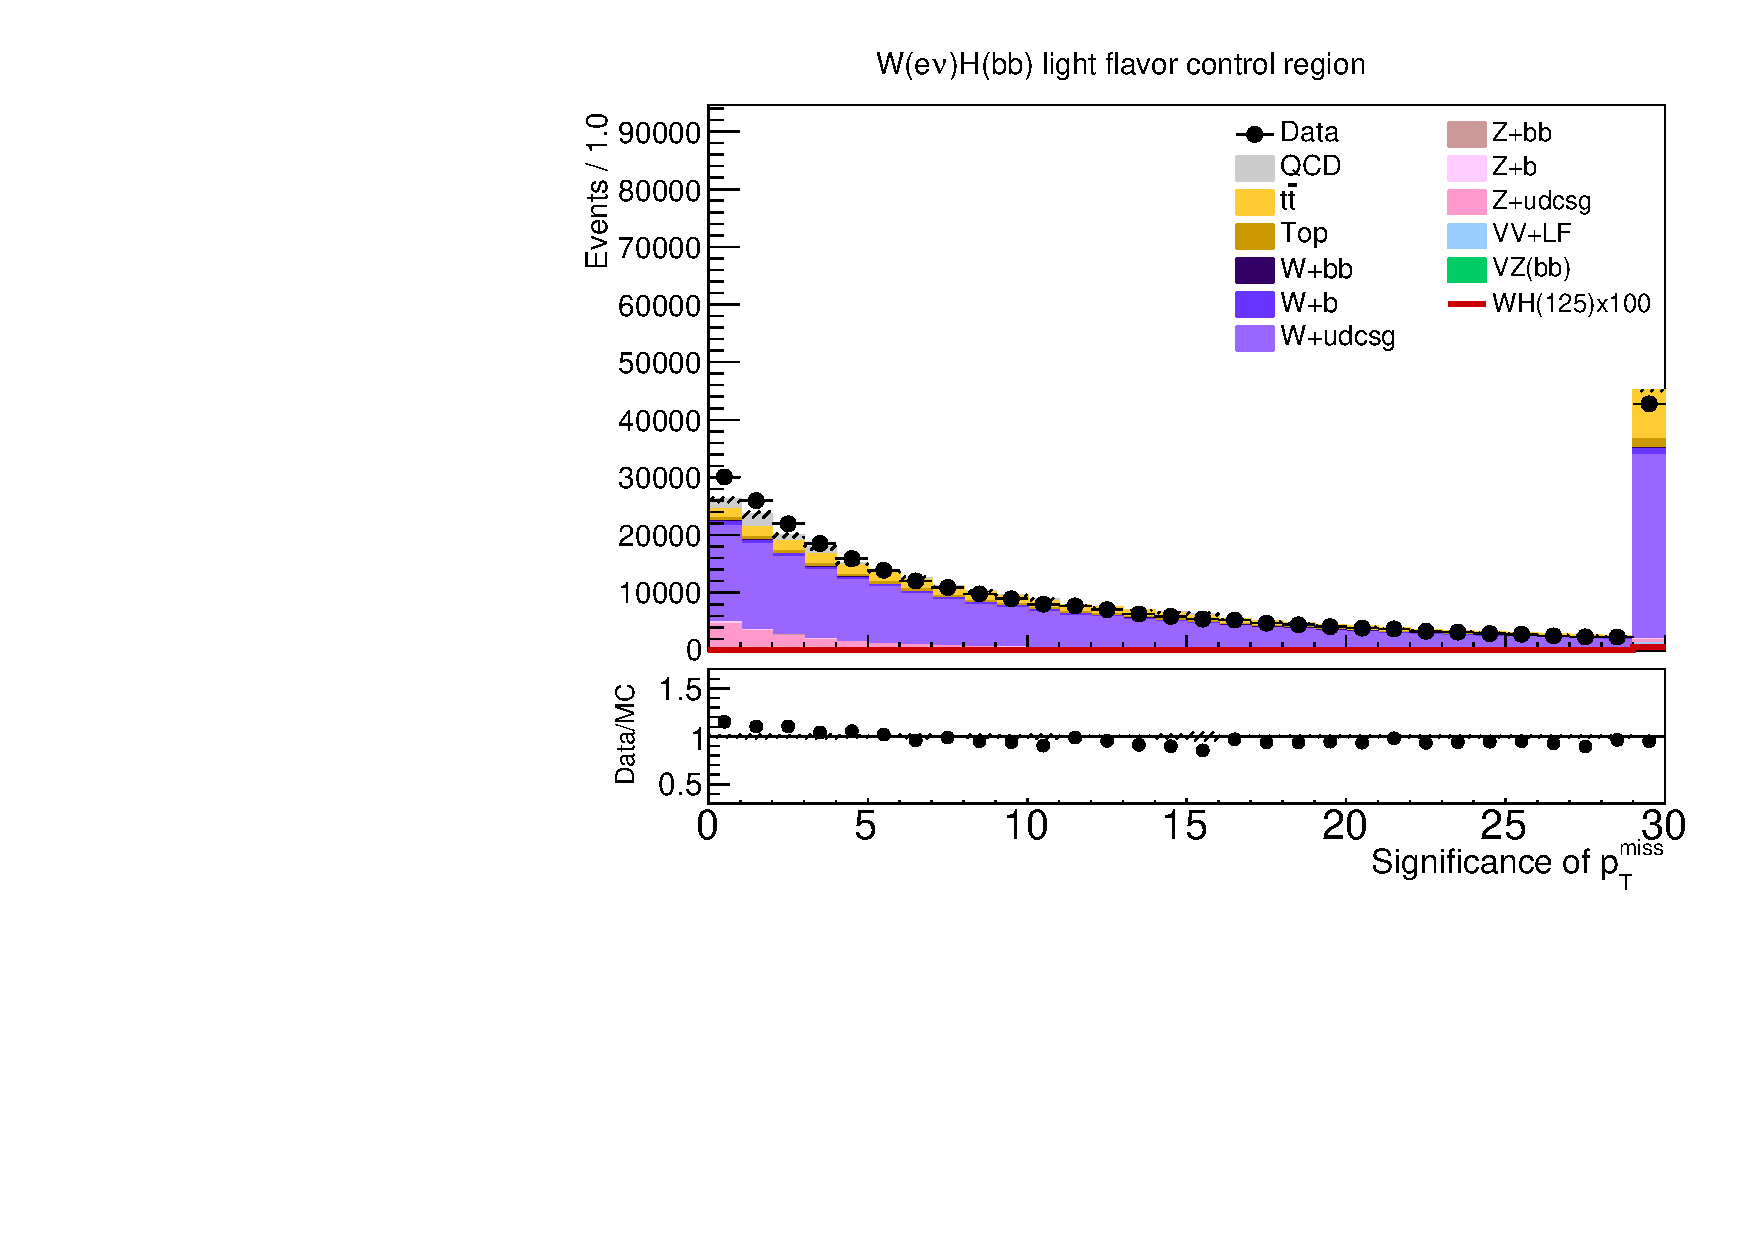
\includegraphics[width=0.48\textwidth]{figures/wlnhbb2016/resolved/WenWHLightFlavorCR_pfmetsig.pdf}
    \caption{W boson reconstruction in the resolved category W(e$\nu$)+LF control region.
    Left to right and top to bottom: electron $\pt$, $\MET$, W boson $\pt$, W boson transverse mass,
    the reconstructed top quark mass, and the $\MET$ significance.
    The simulated shapes are prefit, with the postfit normalizations applied.}
    \label{fig:res_WenLF_WBosons}
  \end{center}
\end{figure}
\clearpage

\begin{figure}[tbp]
  \begin{center}
    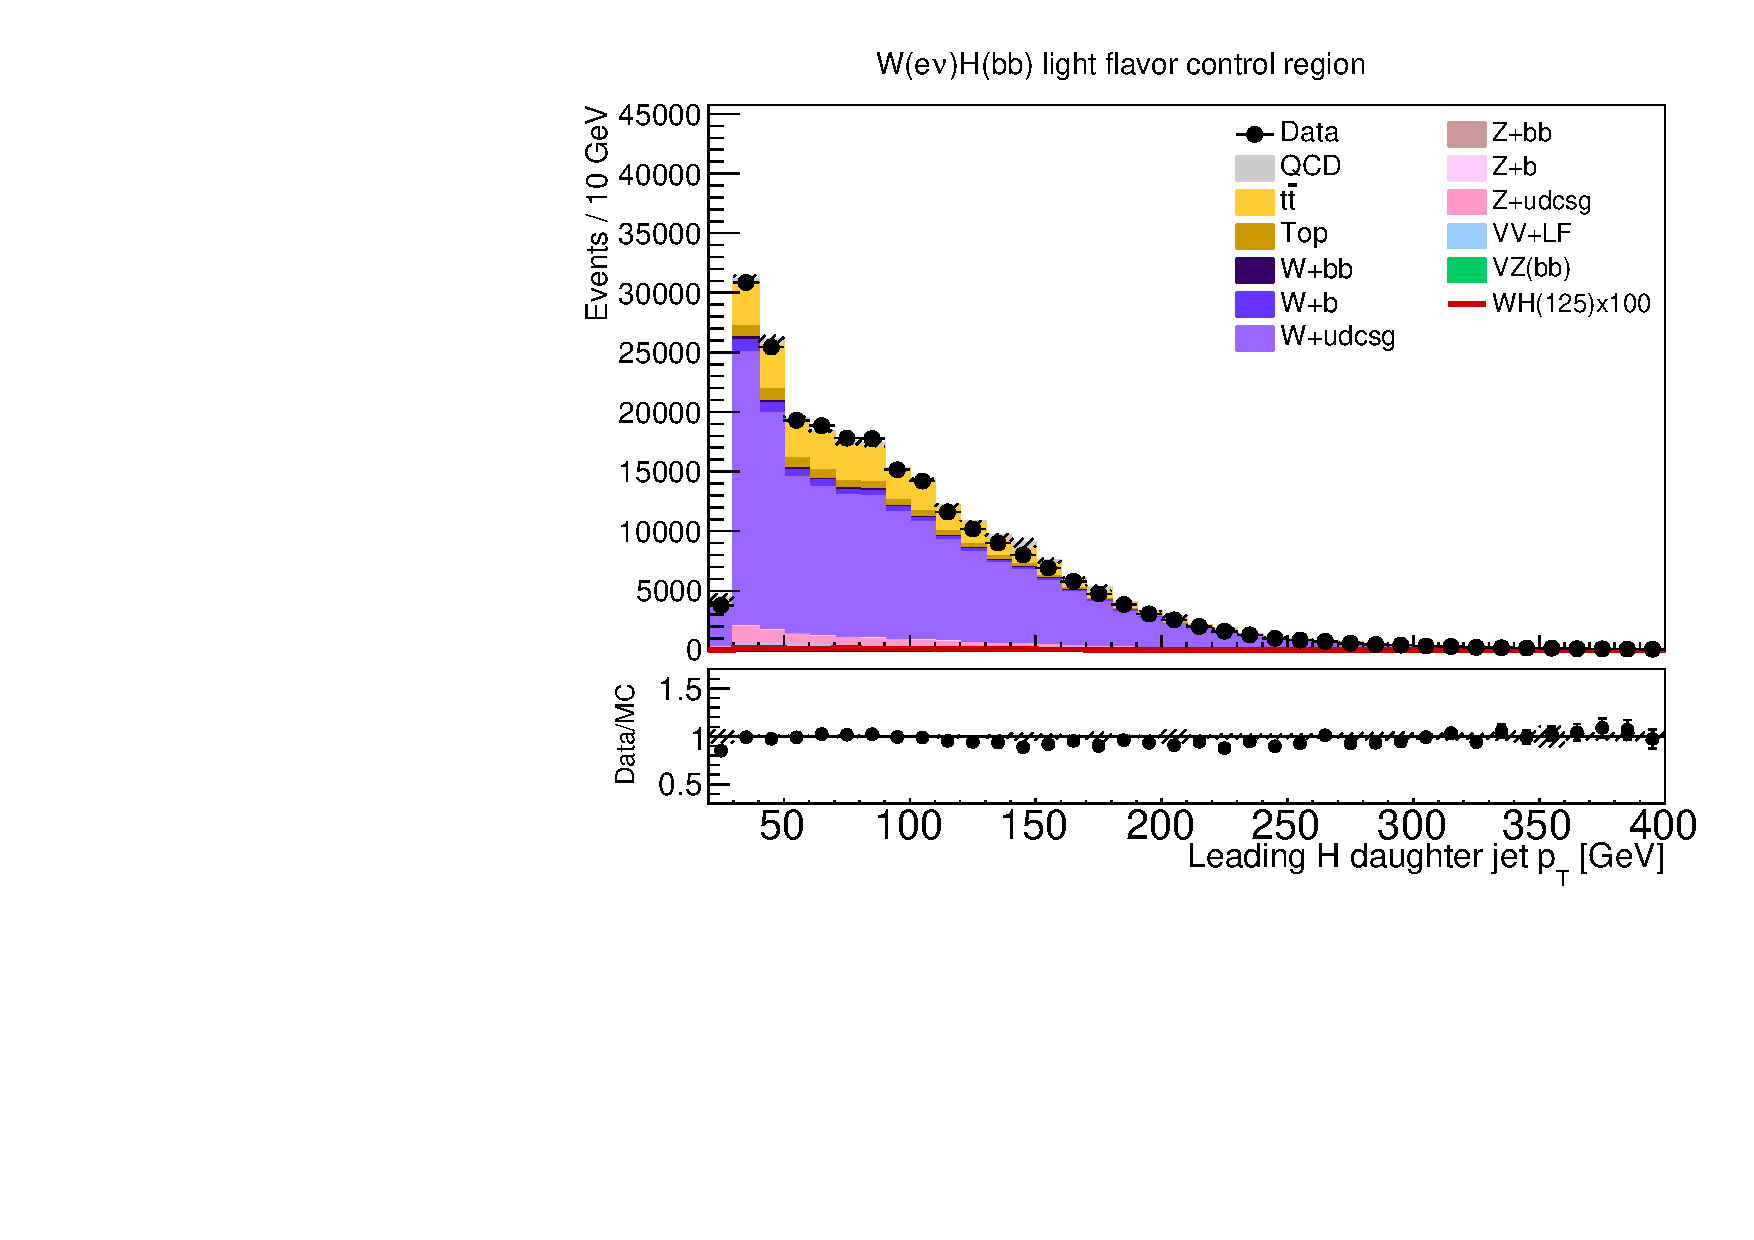
\includegraphics[width=0.48\textwidth]{figures/wlnhbb2016/resolved/WenWHLightFlavorCR_Hbjet1Pt.pdf}
    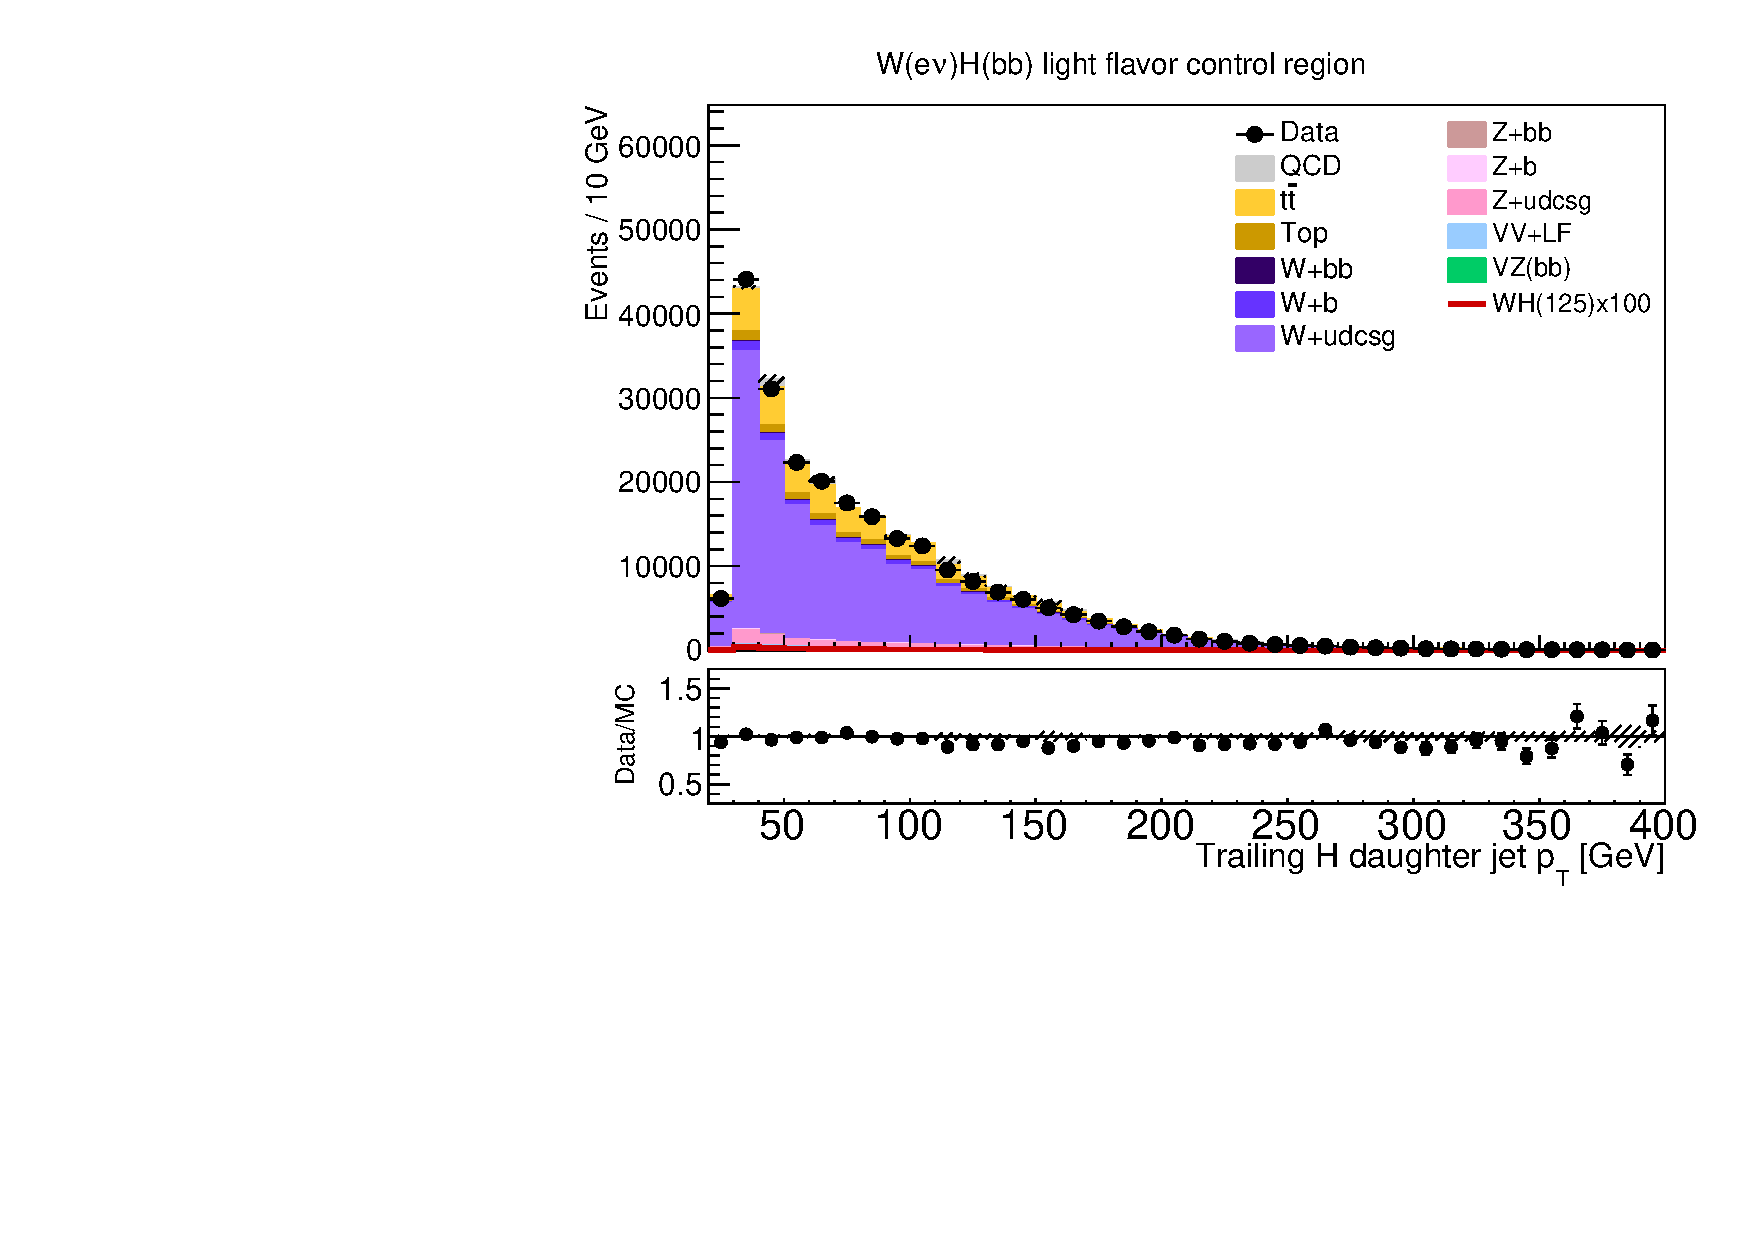
\includegraphics[width=0.48\textwidth]{figures/wlnhbb2016/resolved/WenWHLightFlavorCR_Hbjet2Pt.pdf}
    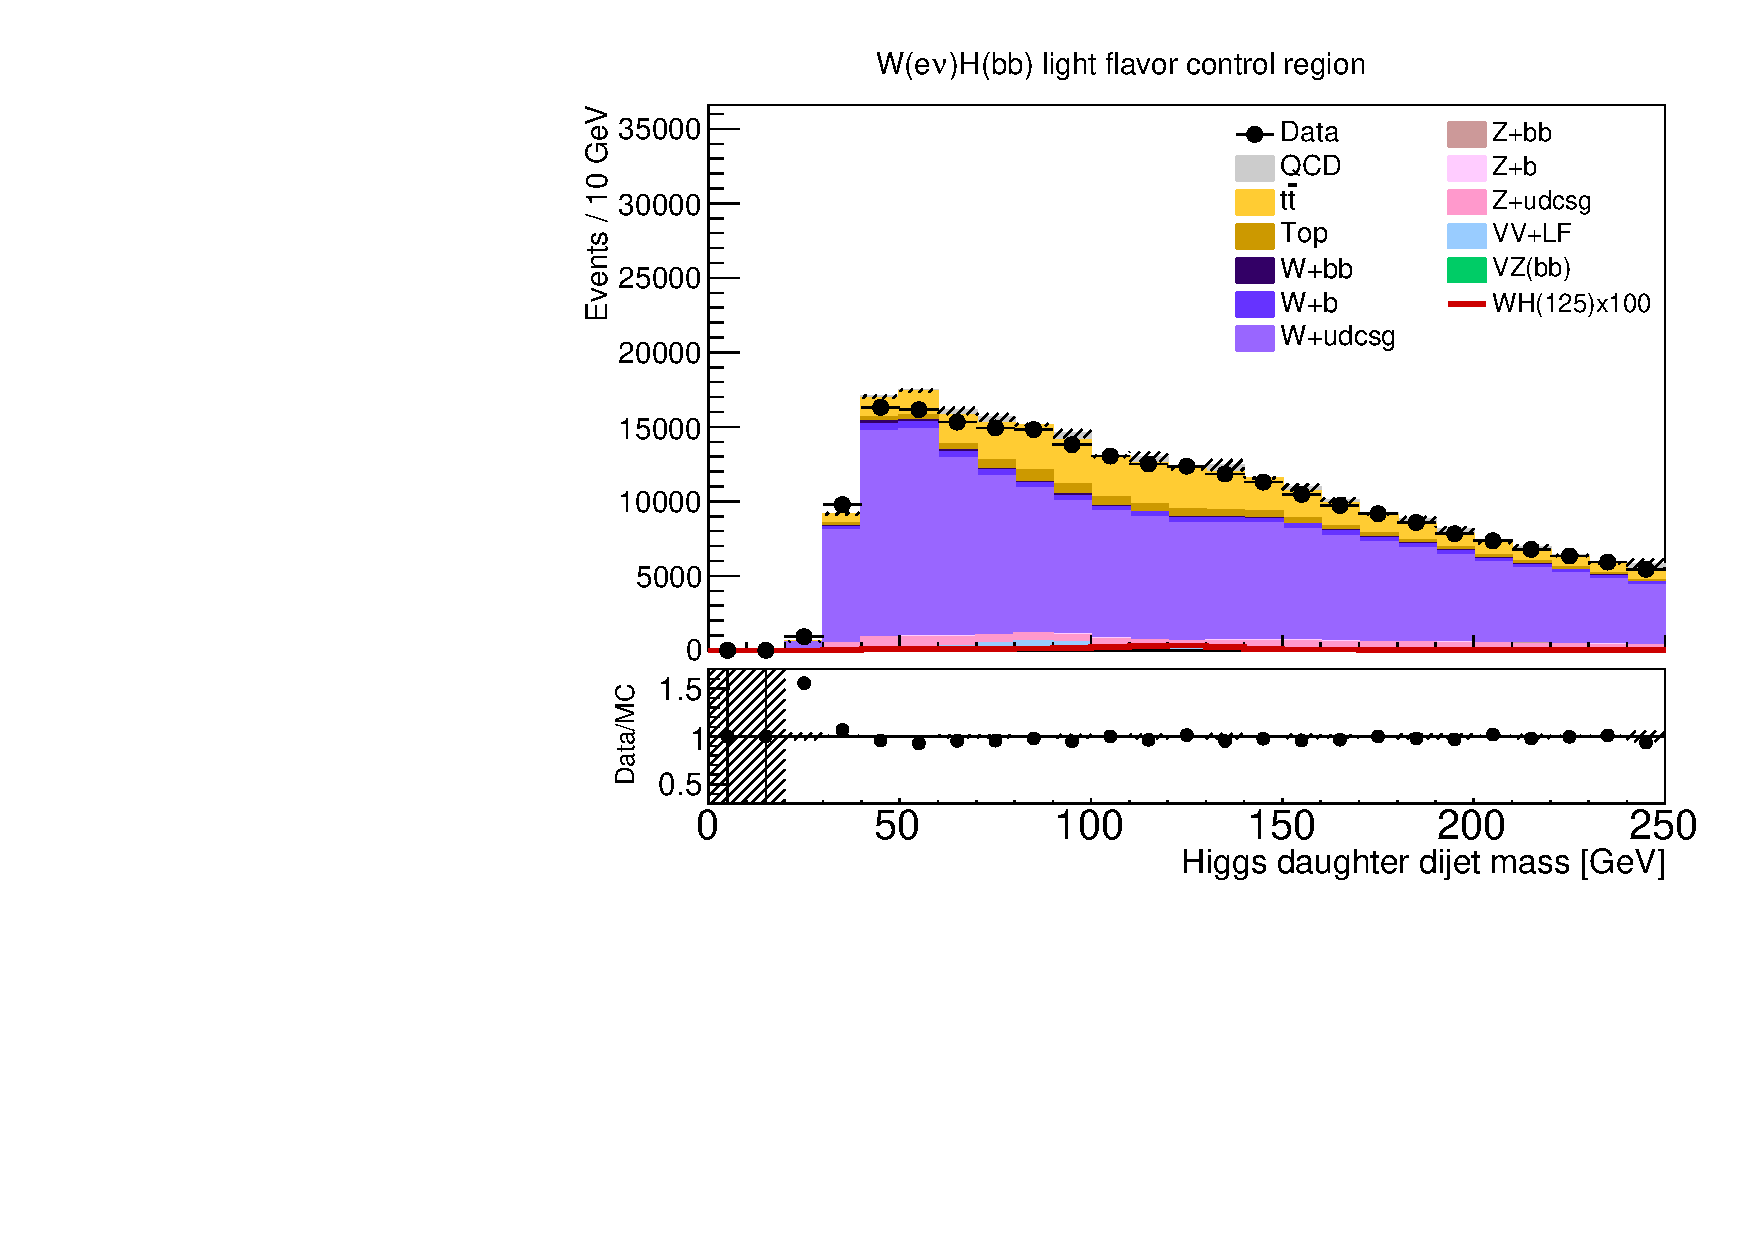
\includegraphics[width=0.48\textwidth]{figures/wlnhbb2016/resolved/WenWHLightFlavorCR_mH.pdf}
    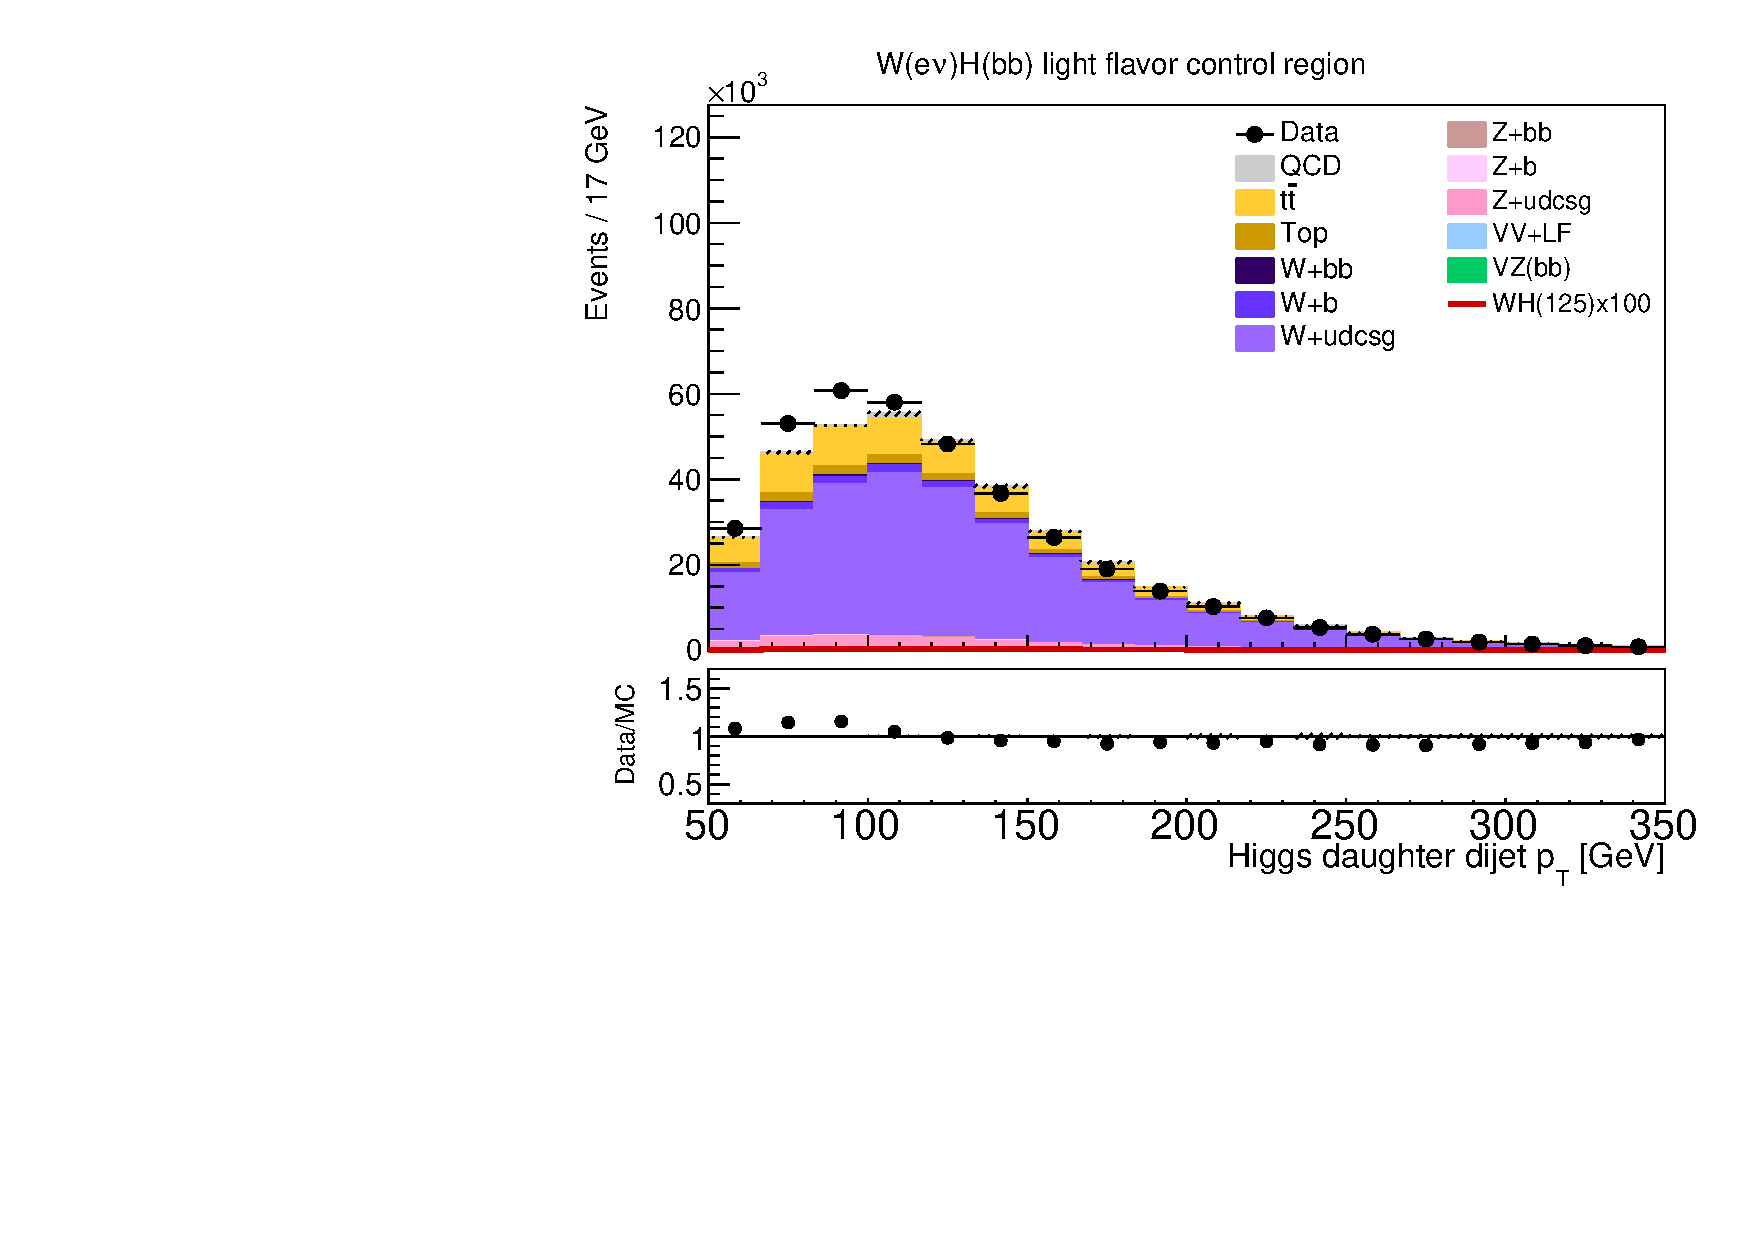
\includegraphics[width=0.48\textwidth]{figures/wlnhbb2016/resolved/WenWHLightFlavorCR_pTH.pdf}
    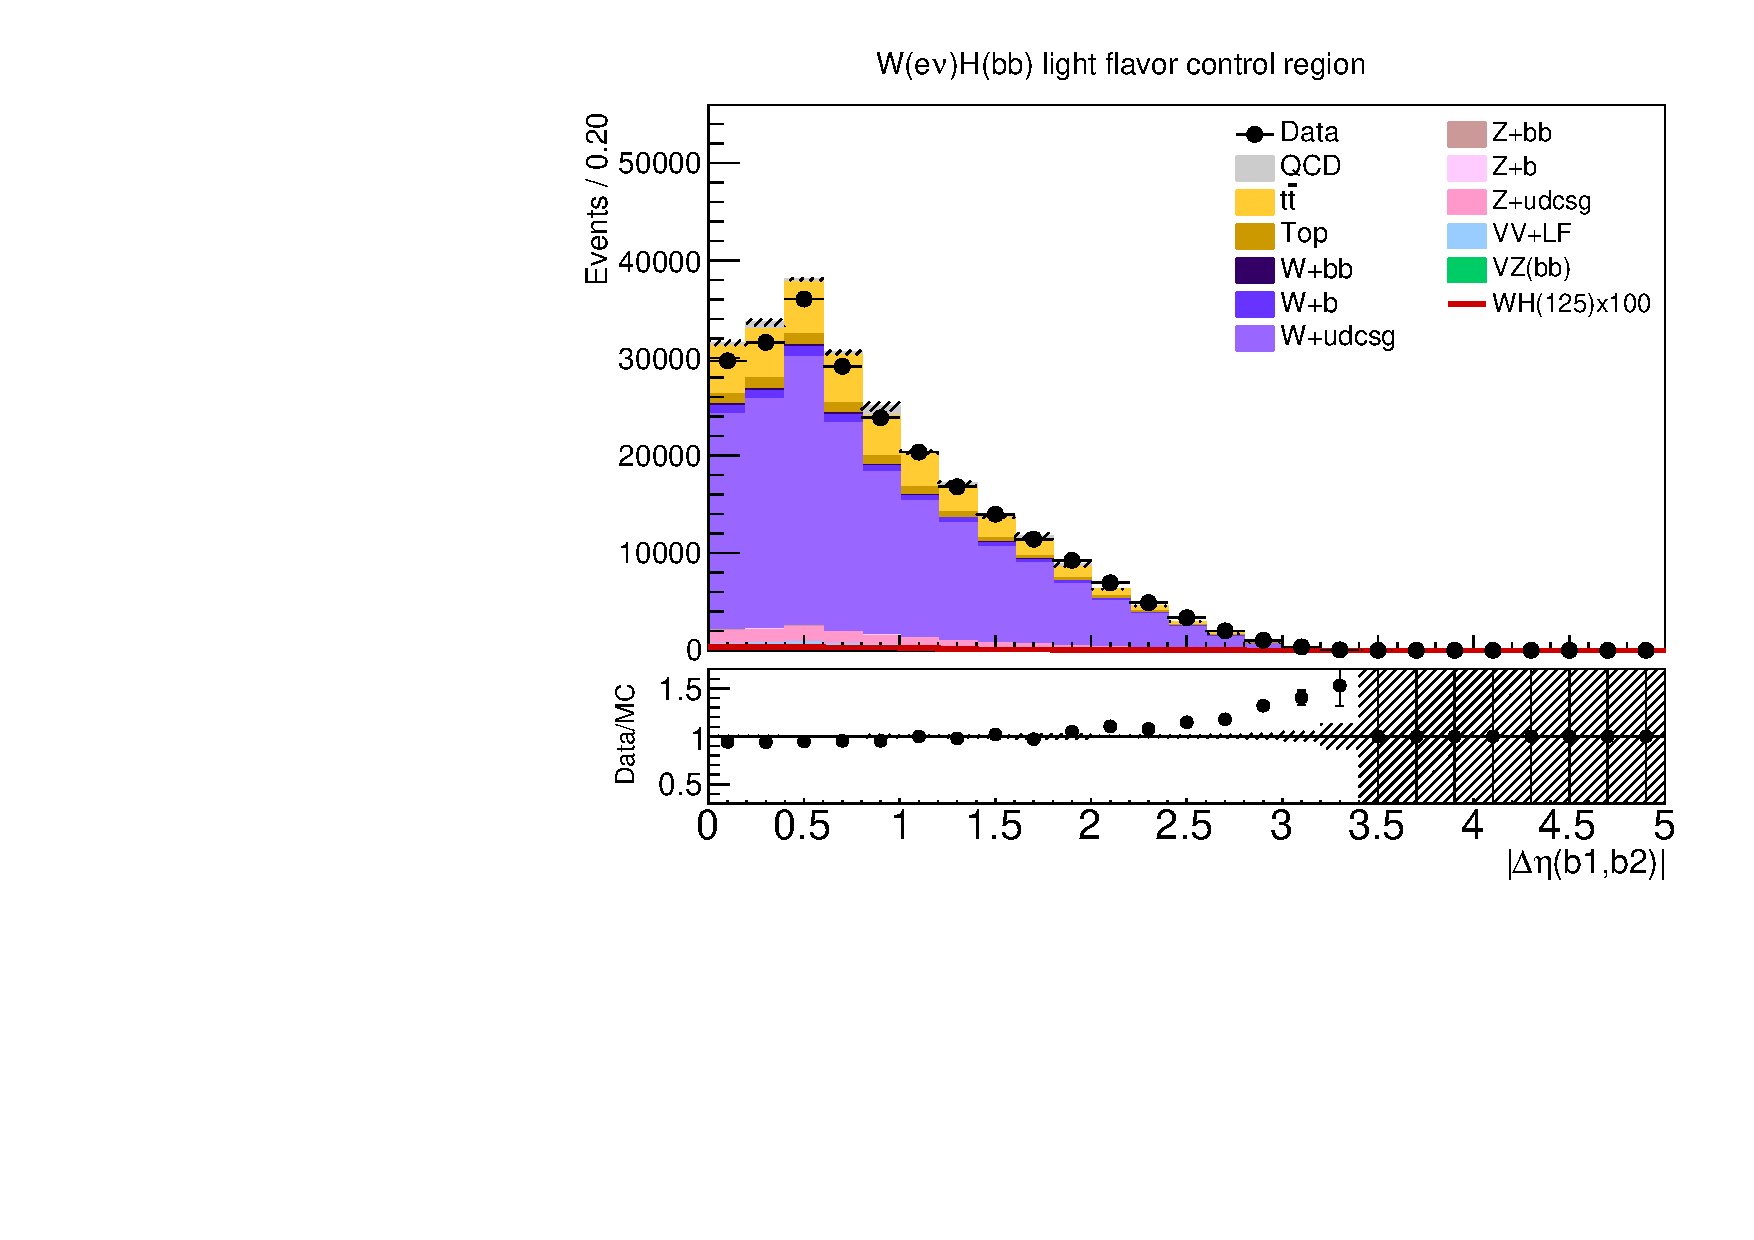
\includegraphics[width=0.48\textwidth]{figures/wlnhbb2016/resolved/WenWHLightFlavorCR_dEtab1b2.pdf}
    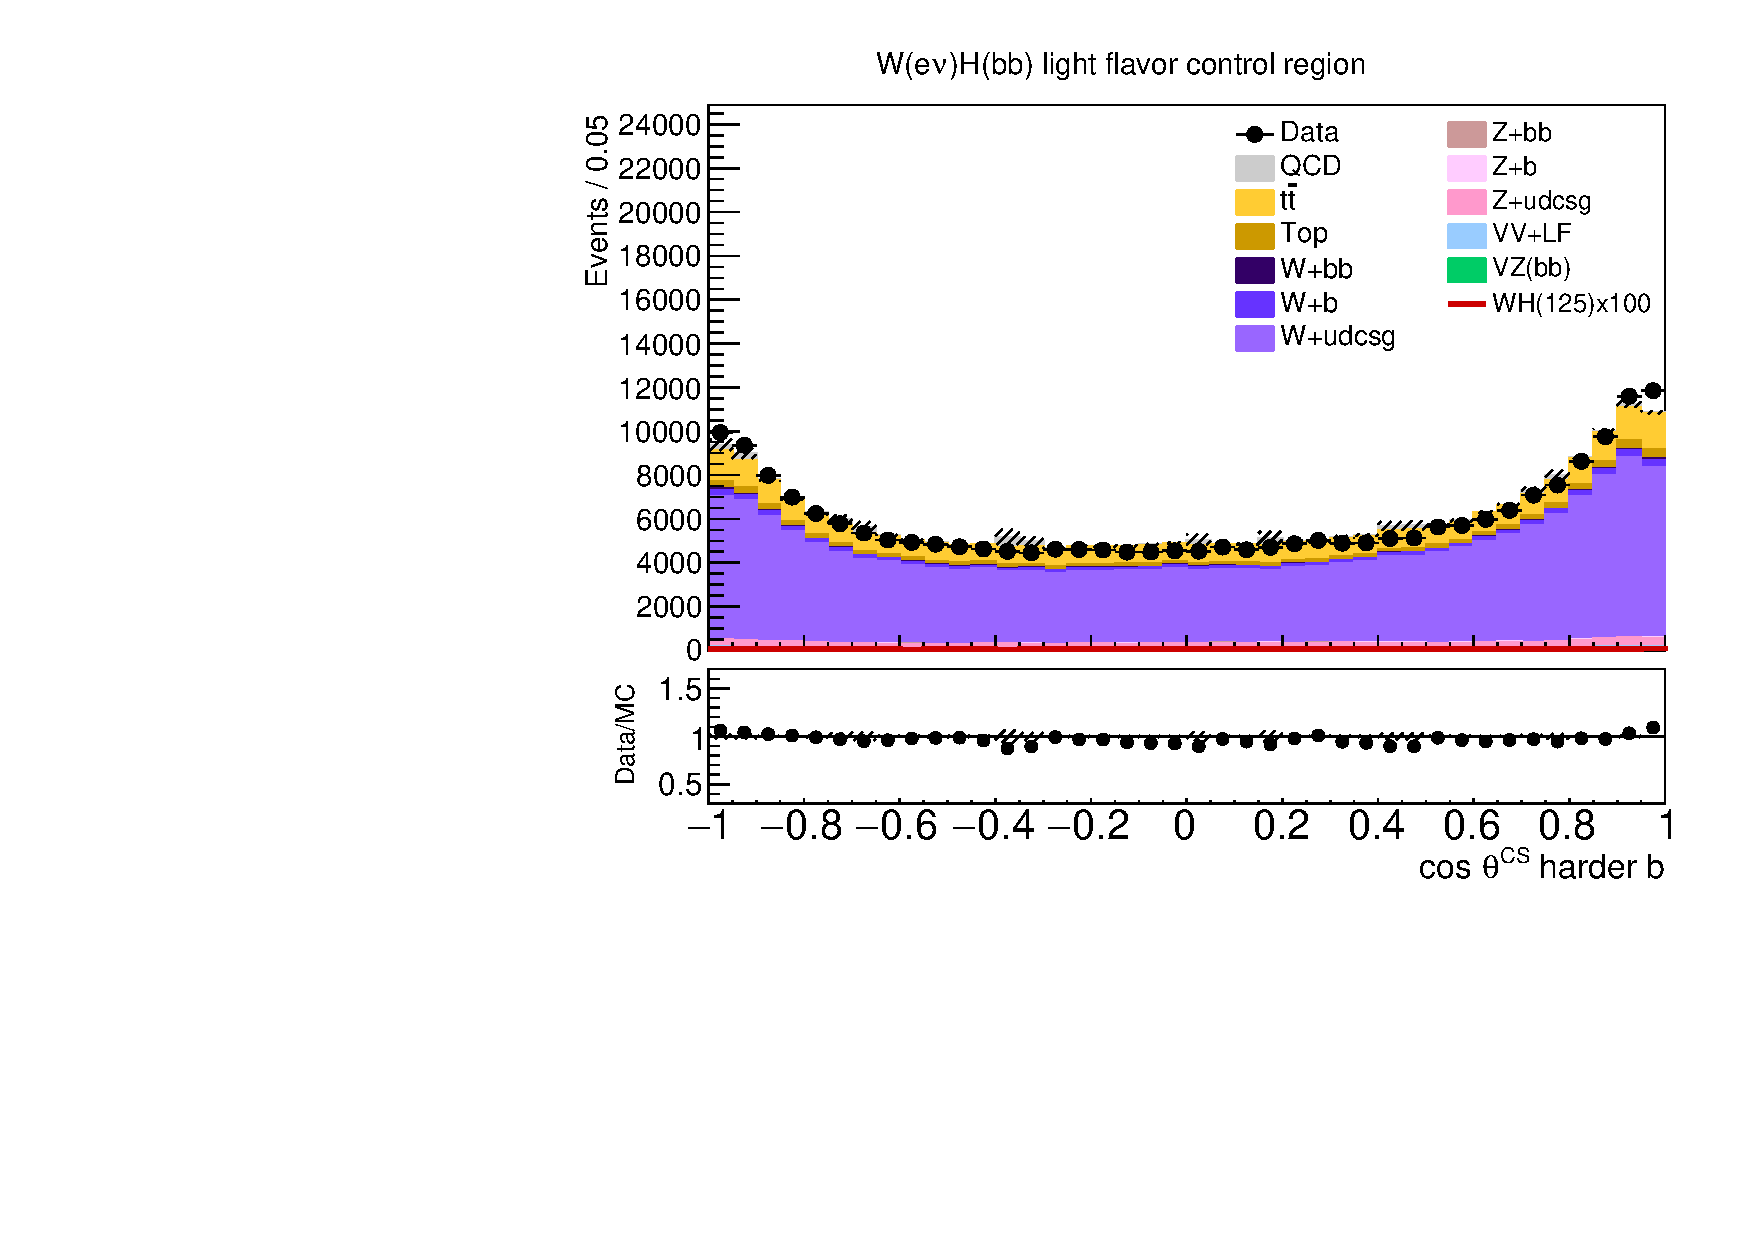
\includegraphics[width=0.48\textwidth]{figures/wlnhbb2016/resolved/WenWHLightFlavorCR_hbbCosThetaCSJ1.pdf}
    \caption{\HBB\ reconstruction in the resolved category W(e$\nu$)+LF control region.
    Left to right and top to bottom: higher b-tagged jet $\pt$, lower b-tagged jet $\pt$, dijet mass, dijet $\pt$, 
    pseudorapidity difference between the two jets, and the Collins-Soper angle of the harder b-tagged jet.
    The simulated shapes are prefit, with the postfit normalizations applied.}
    \label{fig:res_WenLF_Hbb}
  \end{center}
\end{figure}
\clearpage

\begin{figure}[tbp]
  \begin{center}
    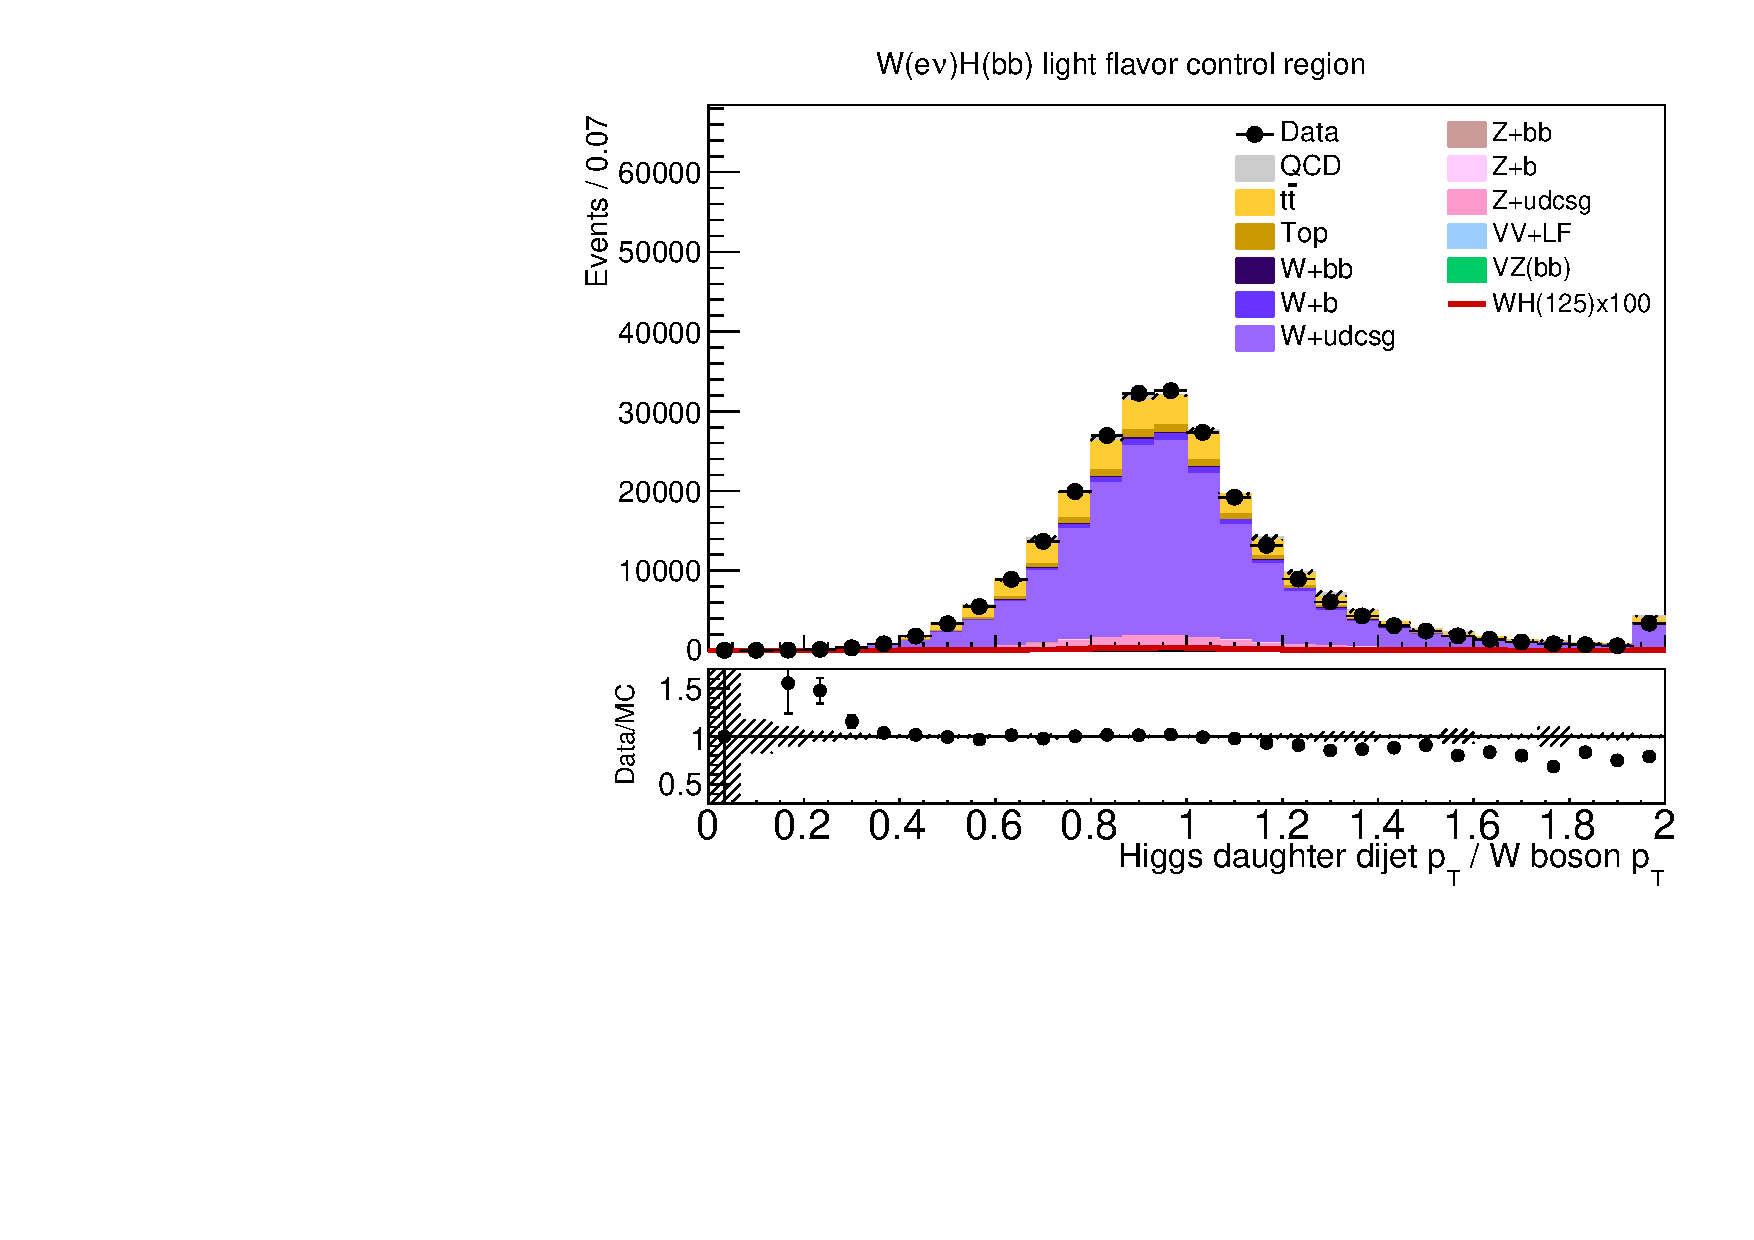
\includegraphics[width=0.48\textwidth]{figures/wlnhbb2016/resolved/WenWHLightFlavorCR_pTBalanceDijetW.pdf}
    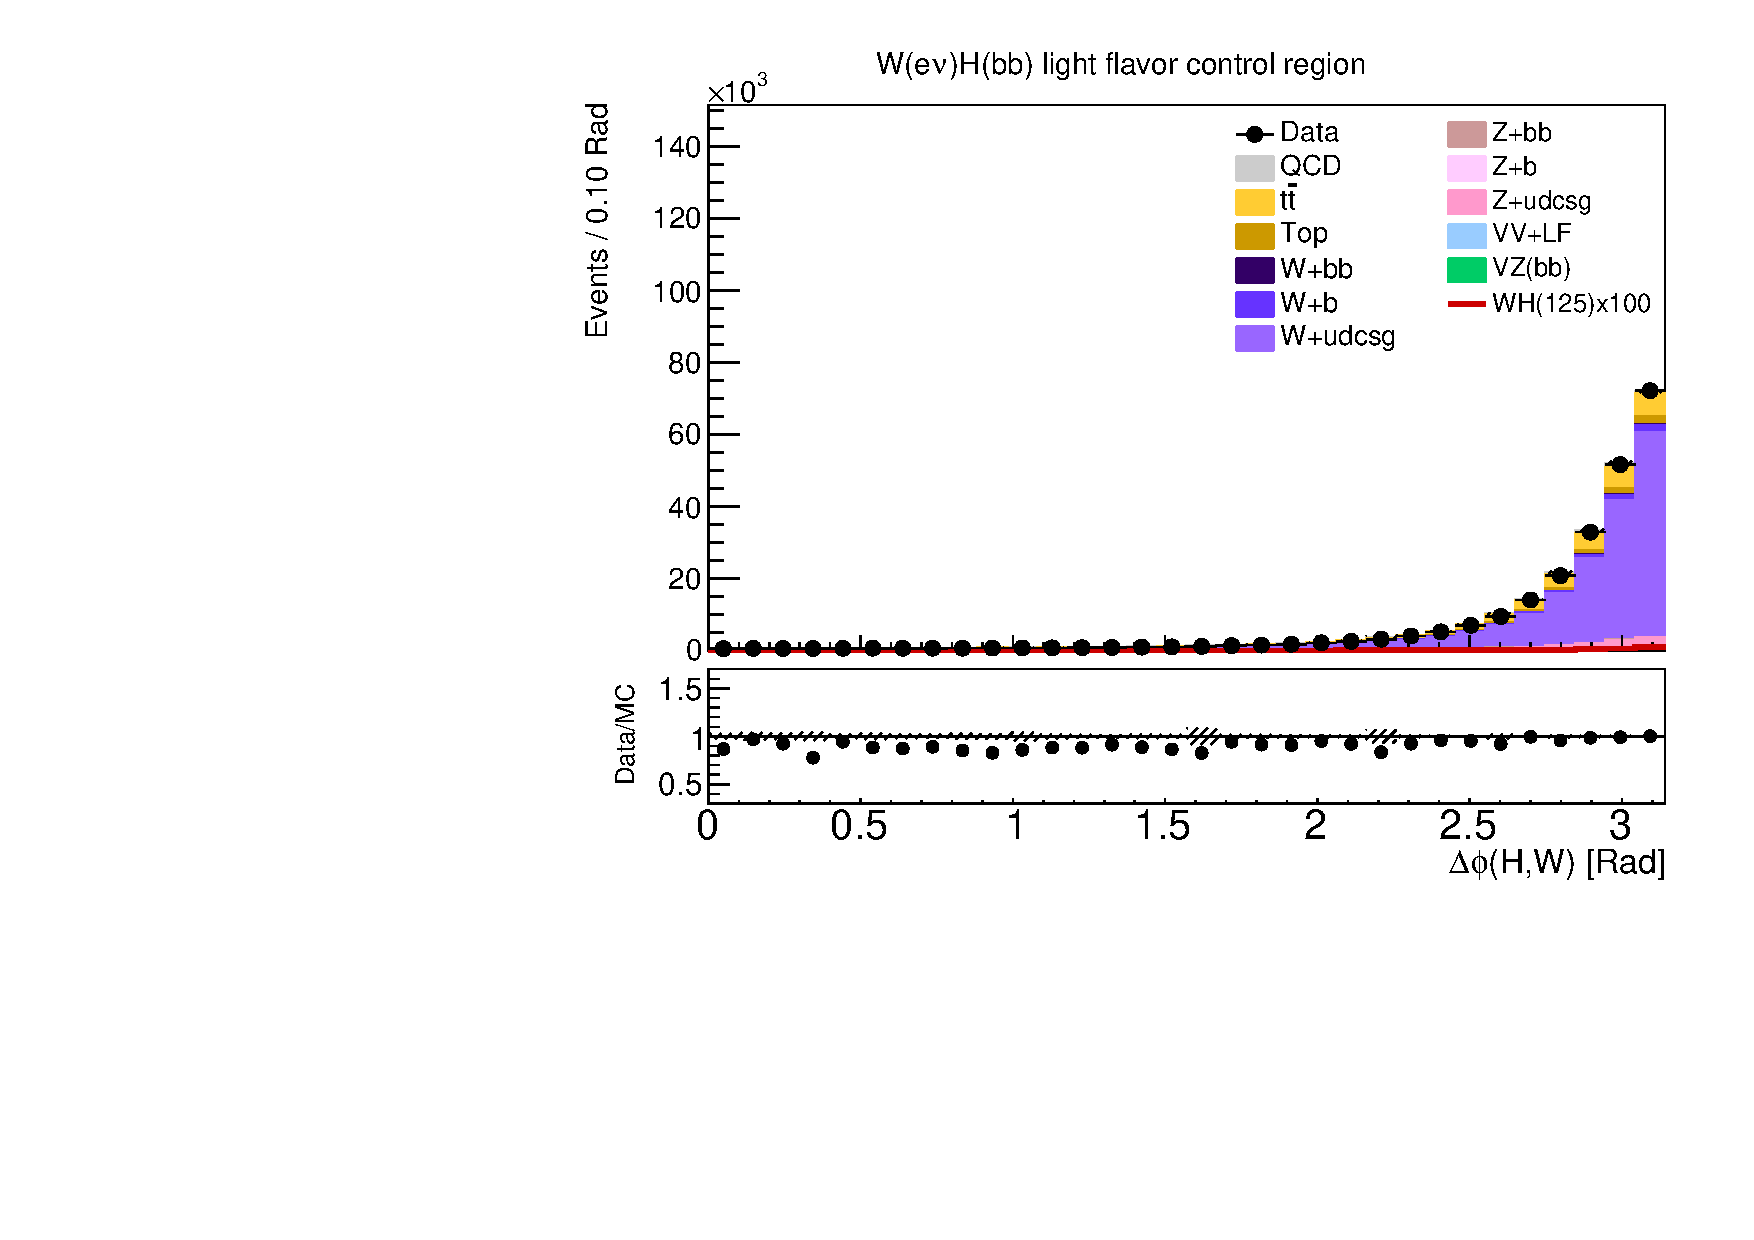
\includegraphics[width=0.48\textwidth]{figures/wlnhbb2016/resolved/WenWHLightFlavorCR_deltaPhiVH.pdf}
    \includegraphics[width=0.48\textwidth]{figures/wlnhbb2016/resolved/WenWHLightFlavorCR_bDiscrMax.pdf}
    \includegraphics[width=0.48\textwidth]{figures/wlnhbb2016/resolved/WenWHLightFlavorCR_nJet.pdf}
    \includegraphics[width=0.48\textwidth]{figures/wlnhbb2016/resolved/WenWHLightFlavorCR_nSoft5.pdf}
    \includegraphics[width=0.48\textwidth]{figures/wlnhbb2016/resolved/WenWHLightFlavorCR_bdtValue.pdf}
    \caption{WH kinematics in the resolved category W(e$\nu$)+LF control region.
    Left to right and top to bottom: WH $\pt$ balance, WH azimuthal separation, leading b-tag score, the number of central jets,
    the number of 5 \GeV\ soft activity jets, and the evaluation of the signal extraction BDT.
    The simulated shapes are prefit, with the postfit normalizations applied.}
    \label{fig:res_WenLF_WH}
  \end{center}
\end{figure}
\clearpage


\begin{figure}[tbp]
  \begin{center}
    \includegraphics[width=0.48\textwidth]{figures/wlnhbb2016/resolved/WmnWHLightFlavorCR_lepton1Pt.pdf}
    \includegraphics[width=0.48\textwidth]{figures/wlnhbb2016/resolved/WmnWHLightFlavorCR_pfmet.pdf}
    \includegraphics[width=0.48\textwidth]{figures/wlnhbb2016/resolved/WmnWHLightFlavorCR_WpT.pdf}
    \includegraphics[width=0.48\textwidth]{figures/wlnhbb2016/resolved/WmnWHLightFlavorCR_mTW.pdf}
    \includegraphics[width=0.48\textwidth]{figures/wlnhbb2016/resolved/WmnWHLightFlavorCR_topMassLep1Met.pdf}
    \includegraphics[width=0.48\textwidth]{figures/wlnhbb2016/resolved/WmnWHLightFlavorCR_pfmetsig.pdf}
    \caption{W boson reconstruction in the resolved category W($\mu\nu$)+LF control region.
    Left to right and top to bottom: muon $\pt$, $\MET$, W boson $\pt$, W boson transverse mass,
    the reconstructed top quark mass, and the $\MET$ significance.
    The simulated shapes are prefit, with the postfit normalizations applied.}
    \label{fig:res_WmnLF_WBosons}
  \end{center}
\end{figure}
\clearpage

\begin{figure}[tbp]
  \begin{center}
    \includegraphics[width=0.48\textwidth]{figures/wlnhbb2016/resolved/WmnWHLightFlavorCR_Hbjet1Pt.pdf}
    \includegraphics[width=0.48\textwidth]{figures/wlnhbb2016/resolved/WmnWHLightFlavorCR_Hbjet2Pt.pdf}
    \includegraphics[width=0.48\textwidth]{figures/wlnhbb2016/resolved/WmnWHLightFlavorCR_mH.pdf}
    \includegraphics[width=0.48\textwidth]{figures/wlnhbb2016/resolved/WmnWHLightFlavorCR_pTH.pdf}
    \includegraphics[width=0.48\textwidth]{figures/wlnhbb2016/resolved/WmnWHLightFlavorCR_dEtab1b2.pdf}
    \includegraphics[width=0.48\textwidth]{figures/wlnhbb2016/resolved/WmnWHLightFlavorCR_hbbCosThetaCSJ1.pdf}
    \caption{\HBB\ reconstruction in the resolved category W($\mu\nu$)+LF control region.
    Left to right and top to bottom: higher b-tagged jet $\pt$, lower b-tagged jet $\pt$, dijet mass, dijet $\pt$, 
    pseudorapidity difference between the two jets, and the Collins-Soper angle of the harder b-tagged jet.
    The simulated shapes are prefit, with the postfit normalizations applied.}
    \label{fig:res_WmnLF_Hbb}
  \end{center}
\end{figure}
\clearpage

\begin{figure}[tbp]
  \begin{center}
    \includegraphics[width=0.48\textwidth]{figures/wlnhbb2016/resolved/WmnWHLightFlavorCR_pTBalanceDijetW.pdf}
    \includegraphics[width=0.48\textwidth]{figures/wlnhbb2016/resolved/WmnWHLightFlavorCR_deltaPhiVH.pdf}
    \includegraphics[width=0.48\textwidth]{figures/wlnhbb2016/resolved/WmnWHLightFlavorCR_bDiscrMax.pdf}
    \includegraphics[width=0.48\textwidth]{figures/wlnhbb2016/resolved/WmnWHLightFlavorCR_nJet.pdf}
    \includegraphics[width=0.48\textwidth]{figures/wlnhbb2016/resolved/WmnWHLightFlavorCR_nSoft5.pdf}
    \includegraphics[width=0.48\textwidth]{figures/wlnhbb2016/resolved/WmnWHLightFlavorCR_bdtValue.pdf}
    \caption{WH kinematics in the resolved category W($\mu\nu$)+LF control region.
    Left to right and top to bottom: WH $\pt$ balance, WH azimuthal separation, leading b-tag score, the number of central jets,
    the number of 5 \GeV\ soft activity jets, and the evaluation of the signal extraction BDT.
    The simulated shapes are prefit, with the postfit normalizations applied.}
    \label{fig:res_WmnLF_WH}
  \end{center}
\end{figure}
\clearpage


\begin{figure}[tbp]
  \begin{center}
    \includegraphics[width=0.48\textwidth]{figures/wlnhbb2016/resolved/WenWH2TopCR_lepton1Pt.pdf}
    \includegraphics[width=0.48\textwidth]{figures/wlnhbb2016/resolved/WenWH2TopCR_pfmet.pdf}
    \includegraphics[width=0.48\textwidth]{figures/wlnhbb2016/resolved/WenWH2TopCR_WpT.pdf}
    \includegraphics[width=0.48\textwidth]{figures/wlnhbb2016/resolved/WenWH2TopCR_mTW.pdf}
    \includegraphics[width=0.48\textwidth]{figures/wlnhbb2016/resolved/WenWH2TopCR_topMassLep1Met.pdf}
    \includegraphics[width=0.48\textwidth]{figures/wlnhbb2016/resolved/WenWH2TopCR_pfmetsig.pdf}
    \caption{W boson reconstruction in the resolved category W(e$\nu$) \ttbar control region.
    Left to right and top to bottom: electron $\pt$, $\MET$, W boson $\pt$, W boson transverse mass,
    the reconstructed top quark mass, and the $\MET$ significance.
    The simulated shapes are prefit, with the postfit normalizations applied.}
    \label{fig:res_WenTT_WBosons}
  \end{center}
\end{figure}
\clearpage

\begin{figure}[tbp]
  \begin{center}
    \includegraphics[width=0.48\textwidth]{figures/wlnhbb2016/resolved/WenWH2TopCR_Hbjet1Pt.pdf}
    \includegraphics[width=0.48\textwidth]{figures/wlnhbb2016/resolved/WenWH2TopCR_Hbjet2Pt.pdf}
    \includegraphics[width=0.48\textwidth]{figures/wlnhbb2016/resolved/WenWH2TopCR_mH.pdf}
    \includegraphics[width=0.48\textwidth]{figures/wlnhbb2016/resolved/WenWH2TopCR_pTH.pdf}
    \includegraphics[width=0.48\textwidth]{figures/wlnhbb2016/resolved/WenWH2TopCR_dEtab1b2.pdf}
    \includegraphics[width=0.48\textwidth]{figures/wlnhbb2016/resolved/WenWH2TopCR_hbbCosThetaCSJ1.pdf}
    \caption{\HBB\ reconstruction in the resolved category W(e$\nu$) \ttbar control region.
    Left to right and top to bottom: higher b-tagged jet $\pt$, lower b-tagged jet $\pt$, dijet mass, dijet $\pt$, 
    pseudorapidity difference between the two jets, and the Collins-Soper angle of the harder b-tagged jet.
    The simulated shapes are prefit, with the postfit normalizations applied.}
    \label{fig:res_WenTT_Hbb}
  \end{center}
\end{figure}
\clearpage

\begin{figure}[tbp]
  \begin{center}
    \includegraphics[width=0.48\textwidth]{figures/wlnhbb2016/resolved/WenWH2TopCR_pTBalanceDijetW.pdf}
    \includegraphics[width=0.48\textwidth]{figures/wlnhbb2016/resolved/WenWH2TopCR_deltaPhiVH.pdf}
    \includegraphics[width=0.48\textwidth]{figures/wlnhbb2016/resolved/WenWH2TopCR_bDiscrMax.pdf}
    \includegraphics[width=0.48\textwidth]{figures/wlnhbb2016/resolved/WenWH2TopCR_nJet.pdf}
    \includegraphics[width=0.48\textwidth]{figures/wlnhbb2016/resolved/WenWH2TopCR_nSoft5.pdf}
    \includegraphics[width=0.48\textwidth]{figures/wlnhbb2016/resolved/WenWH2TopCR_bdtValue.pdf}
    \caption{WH kinematics in the resolved category W(e$\nu$) \ttbar control region.
    Left to right and top to bottom: WH $\pt$ balance, WH azimuthal separation, leading b-tag score, the number of central jets,
    the number of 5 \GeV\ soft activity jets, and the evaluation of the signal extraction BDT.
    The simulated shapes are prefit, with the postfit normalizations applied.}
    \label{fig:res_WenTT_WH}
  \end{center}
\end{figure}
\clearpage


\begin{figure}[tbp]
  \begin{center}
    \includegraphics[width=0.48\textwidth]{figures/wlnhbb2016/resolved/WmnWH2TopCR_lepton1Pt.pdf}
    \includegraphics[width=0.48\textwidth]{figures/wlnhbb2016/resolved/WmnWH2TopCR_pfmet.pdf}
    \includegraphics[width=0.48\textwidth]{figures/wlnhbb2016/resolved/WmnWH2TopCR_WpT.pdf}
    \includegraphics[width=0.48\textwidth]{figures/wlnhbb2016/resolved/WmnWH2TopCR_mTW.pdf}
    \includegraphics[width=0.48\textwidth]{figures/wlnhbb2016/resolved/WmnWH2TopCR_topMassLep1Met.pdf}
    \includegraphics[width=0.48\textwidth]{figures/wlnhbb2016/resolved/WmnWH2TopCR_pfmetsig.pdf}
    \caption{W boson reconstruction in the resolved category W($\mu\nu$) \ttbar control region.
    Left to right and top to bottom: muon $\pt$, $\MET$, W boson $\pt$, W boson transverse mass,
    the reconstructed top quark mass, and the $\MET$ significance.
    The simulated shapes are prefit, with the postfit normalizations applied.}
    \label{fig:res_WmnTT_WBosons}
  \end{center}
\end{figure}
\clearpage

\begin{figure}[tbp]
  \begin{center}
    \includegraphics[width=0.48\textwidth]{figures/wlnhbb2016/resolved/WmnWH2TopCR_Hbjet1Pt.pdf}
    \includegraphics[width=0.48\textwidth]{figures/wlnhbb2016/resolved/WmnWH2TopCR_Hbjet2Pt.pdf}
    \includegraphics[width=0.48\textwidth]{figures/wlnhbb2016/resolved/WmnWH2TopCR_mH.pdf}
    \includegraphics[width=0.48\textwidth]{figures/wlnhbb2016/resolved/WmnWH2TopCR_pTH.pdf}
    \includegraphics[width=0.48\textwidth]{figures/wlnhbb2016/resolved/WmnWH2TopCR_dEtab1b2.pdf}
    \includegraphics[width=0.48\textwidth]{figures/wlnhbb2016/resolved/WmnWH2TopCR_hbbCosThetaCSJ1.pdf}
    \caption{\HBB\ reconstruction in the resolved category W($\mu\nu$) \ttbar control region.
    Left to right and top to bottom: higher b-tagged jet $\pt$, lower b-tagged jet $\pt$, dijet mass, dijet $\pt$, 
    pseudorapidity difference between the two jets, and the Collins-Soper angle of the harder b-tagged jet.
    The simulated shapes are prefit, with the postfit normalizations applied.}
    \label{fig:res_WmnTT_Hbb}
  \end{center}
\end{figure}
\clearpage

\begin{figure}[tbp]
  \begin{center}
    \includegraphics[width=0.48\textwidth]{figures/wlnhbb2016/resolved/WmnWH2TopCR_pTBalanceDijetW.pdf}
    \includegraphics[width=0.48\textwidth]{figures/wlnhbb2016/resolved/WmnWH2TopCR_deltaPhiVH.pdf}
    \includegraphics[width=0.48\textwidth]{figures/wlnhbb2016/resolved/WmnWH2TopCR_bDiscrMax.pdf}
    \includegraphics[width=0.48\textwidth]{figures/wlnhbb2016/resolved/WmnWH2TopCR_nJet.pdf}
    \includegraphics[width=0.48\textwidth]{figures/wlnhbb2016/resolved/WmnWH2TopCR_nSoft5.pdf}
    \includegraphics[width=0.48\textwidth]{figures/wlnhbb2016/resolved/WmnWH2TopCR_bdtValue.pdf}
    \caption{WH kinematics in the resolved category W($\mu\nu$) \ttbar control region.
    Left to right and top to bottom: WH $\pt$ balance, WH azimuthal separation, leading b-tag score, the number of central jets,
    the number of 5 \GeV\ soft activity jets, and the evaluation of the signal extraction BDT.
    The simulated shapes are prefit, with the postfit normalizations applied.}
    \label{fig:res_WmnTT_WH}
  \end{center}
\end{figure}
\clearpage

\begin{figure}[tbp]
  \begin{center}
    \includegraphics[width=0.48\textwidth]{figures/wlnhbb2016/resolved/WenWHHeavyFlavorCRLowMass_lepton1Pt.pdf}
    \includegraphics[width=0.48\textwidth]{figures/wlnhbb2016/resolved/WenWHHeavyFlavorCRLowMass_pfmet.pdf}
    \includegraphics[width=0.48\textwidth]{figures/wlnhbb2016/resolved/WenWHHeavyFlavorCRLowMass_WpT.pdf}
    \includegraphics[width=0.48\textwidth]{figures/wlnhbb2016/resolved/WenWHHeavyFlavorCRLowMass_mTW.pdf}
    \includegraphics[width=0.48\textwidth]{figures/wlnhbb2016/resolved/WenWHHeavyFlavorCRLowMass_topMassLep1Met.pdf}
    \includegraphics[width=0.48\textwidth]{figures/wlnhbb2016/resolved/WenWHHeavyFlavorCRLowMass_pfmetsig.pdf}
    \caption{W boson reconstruction in the resolved category W(e$\nu$)+HF low mass control region.
    Left to right and top to bottom: electron $\pt$, $\MET$, W boson $\pt$, W boson transverse mass,
    the reconstructed top quark mass, and the $\MET$ significance.
    The simulated shapes are prefit, with the postfit normalizations applied.}
    \label{fig:res_WenHFLowMass_WBosons}
  \end{center}
\end{figure}
\clearpage

\begin{figure}[tbp]
  \begin{center}
    \includegraphics[width=0.48\textwidth]{figures/wlnhbb2016/resolved/WenWHHeavyFlavorCRLowMass_Hbjet1Pt.pdf}
    \includegraphics[width=0.48\textwidth]{figures/wlnhbb2016/resolved/WenWHHeavyFlavorCRLowMass_Hbjet2Pt.pdf}
    \includegraphics[width=0.48\textwidth]{figures/wlnhbb2016/resolved/WenWHHeavyFlavorCRLowMass_mH.pdf}
    \includegraphics[width=0.48\textwidth]{figures/wlnhbb2016/resolved/WenWHHeavyFlavorCRLowMass_pTH.pdf}
    \includegraphics[width=0.48\textwidth]{figures/wlnhbb2016/resolved/WenWHHeavyFlavorCRLowMass_dEtab1b2.pdf}
    \includegraphics[width=0.48\textwidth]{figures/wlnhbb2016/resolved/WenWHHeavyFlavorCRLowMass_hbbCosThetaCSJ1.pdf}
    \caption{\HBB\ reconstruction in the resolved category W(e$\nu$)+HF low mass control region.
    Left to right and top to bottom: higher b-tagged jet $\pt$, lower b-tagged jet $\pt$, dijet mass, dijet $\pt$, 
    pseudorapidity difference between the two jets, and the Collins-Soper angle of the harder b-tagged jet.
    The simulated shapes are prefit, with the postfit normalizations applied.}
    \label{fig:res_WenHFLowMass_Hbb}
  \end{center}
\end{figure}
\clearpage

\begin{figure}[tbp]
  \begin{center}
    \includegraphics[width=0.48\textwidth]{figures/wlnhbb2016/resolved/WenWHHeavyFlavorCRLowMass_pTBalanceDijetW.pdf}
    \includegraphics[width=0.48\textwidth]{figures/wlnhbb2016/resolved/WenWHHeavyFlavorCRLowMass_deltaPhiVH.pdf}
    \includegraphics[width=0.48\textwidth]{figures/wlnhbb2016/resolved/WenWHHeavyFlavorCRLowMass_bDiscrMax.pdf}
    \includegraphics[width=0.48\textwidth]{figures/wlnhbb2016/resolved/WenWHHeavyFlavorCRLowMass_nJet.pdf}
    \includegraphics[width=0.48\textwidth]{figures/wlnhbb2016/resolved/WenWHHeavyFlavorCRLowMass_nSoft5.pdf}
    \includegraphics[width=0.48\textwidth]{figures/wlnhbb2016/resolved/WenWHHeavyFlavorCRLowMass_bdtValue.pdf}
    \caption{WH kinematics in the resolved category W(e$\nu$)+HF low mass control region.
    Left to right and top to bottom: WH $\pt$ balance, WH azimuthal separation, leading b-tag score, the number of central jets,
    the number of 5 \GeV\ soft activity jets, and the evaluation of the signal extraction BDT.
    The simulated shapes are prefit, with the postfit normalizations applied.}
    \label{fig:res_WenHFLowMass_WH}
  \end{center}
\end{figure}
\clearpage


\begin{figure}[tbp]
  \begin{center}
    \includegraphics[width=0.48\textwidth]{figures/wlnhbb2016/resolved/WmnWHHeavyFlavorCRLowMass_lepton1Pt.pdf}
    \includegraphics[width=0.48\textwidth]{figures/wlnhbb2016/resolved/WmnWHHeavyFlavorCRLowMass_pfmet.pdf}
    \includegraphics[width=0.48\textwidth]{figures/wlnhbb2016/resolved/WmnWHHeavyFlavorCRLowMass_WpT.pdf}
    \includegraphics[width=0.48\textwidth]{figures/wlnhbb2016/resolved/WmnWHHeavyFlavorCRLowMass_mTW.pdf}
    \includegraphics[width=0.48\textwidth]{figures/wlnhbb2016/resolved/WmnWHHeavyFlavorCRLowMass_topMassLep1Met.pdf}
    \includegraphics[width=0.48\textwidth]{figures/wlnhbb2016/resolved/WmnWHHeavyFlavorCRLowMass_pfmetsig.pdf}
    \caption{W boson reconstruction in the resolved category W($\mu\nu$)+HF low mass control region.
    Left to right and top to bottom: muon $\pt$, $\MET$, W boson $\pt$, W boson transverse mass,
    the reconstructed top quark mass, and the $\MET$ significance.
    The simulated shapes are prefit, with the postfit normalizations applied.}
    \label{fig:res_WmnHFLowMass_WBosons}
  \end{center}
\end{figure}
\clearpage

\begin{figure}[tbp]
  \begin{center}
    \includegraphics[width=0.48\textwidth]{figures/wlnhbb2016/resolved/WmnWHHeavyFlavorCRLowMass_Hbjet1Pt.pdf}
    \includegraphics[width=0.48\textwidth]{figures/wlnhbb2016/resolved/WmnWHHeavyFlavorCRLowMass_Hbjet2Pt.pdf}
    \includegraphics[width=0.48\textwidth]{figures/wlnhbb2016/resolved/WmnWHHeavyFlavorCRLowMass_mH.pdf}
    \includegraphics[width=0.48\textwidth]{figures/wlnhbb2016/resolved/WmnWHHeavyFlavorCRLowMass_pTH.pdf}
    \includegraphics[width=0.48\textwidth]{figures/wlnhbb2016/resolved/WmnWHHeavyFlavorCRLowMass_dEtab1b2.pdf}
    \includegraphics[width=0.48\textwidth]{figures/wlnhbb2016/resolved/WmnWHHeavyFlavorCRLowMass_hbbCosThetaCSJ1.pdf}
    \caption{\HBB\ reconstruction in the resolved category W($\mu\nu$)+HF low mass control region.
    Left to right and top to bottom: higher b-tagged jet $\pt$, lower b-tagged jet $\pt$, dijet mass, dijet $\pt$, 
    pseudorapidity difference between the two jets, and the Collins-Soper angle of the harder b-tagged jet.
    The simulated shapes are prefit, with the postfit normalizations applied.}
    \label{fig:res_WmnHFLowMass_Hbb}
  \end{center}
\end{figure}
\clearpage

\begin{figure}[tbp]
  \begin{center}
    \includegraphics[width=0.48\textwidth]{figures/wlnhbb2016/resolved/WmnWHHeavyFlavorCRLowMass_pTBalanceDijetW.pdf}
    \includegraphics[width=0.48\textwidth]{figures/wlnhbb2016/resolved/WmnWHHeavyFlavorCRLowMass_deltaPhiVH.pdf}
    \includegraphics[width=0.48\textwidth]{figures/wlnhbb2016/resolved/WmnWHHeavyFlavorCRLowMass_bDiscrMax.pdf}
    \includegraphics[width=0.48\textwidth]{figures/wlnhbb2016/resolved/WmnWHHeavyFlavorCRLowMass_nJet.pdf}
    \includegraphics[width=0.48\textwidth]{figures/wlnhbb2016/resolved/WmnWHHeavyFlavorCRLowMass_nSoft5.pdf}
    \includegraphics[width=0.48\textwidth]{figures/wlnhbb2016/resolved/WmnWHHeavyFlavorCRLowMass_bdtValue.pdf}
    \caption{WH kinematics in the resolved category W($\mu\nu$)+HF low mass control region.
    Left to right and top to bottom: WH $\pt$ balance, WH azimuthal separation, leading b-tag score, the number of central jets,
    the number of 5 \GeV\ soft activity jets, and the evaluation of the signal extraction BDT.
    The simulated shapes are prefit, with the postfit normalizations applied.}
    \label{fig:res_WmnHFLowMass_WH}
  \end{center}
\end{figure}
\clearpage

\begin{figure}[tbp]
  \begin{center}
    \includegraphics[width=0.48\textwidth]{figures/wlnhbb2016/resolved/WenWHHeavyFlavorCRHighMass_lepton1Pt.pdf}
    \includegraphics[width=0.48\textwidth]{figures/wlnhbb2016/resolved/WenWHHeavyFlavorCRHighMass_pfmet.pdf}
    \includegraphics[width=0.48\textwidth]{figures/wlnhbb2016/resolved/WenWHHeavyFlavorCRHighMass_WpT.pdf}
    \includegraphics[width=0.48\textwidth]{figures/wlnhbb2016/resolved/WenWHHeavyFlavorCRHighMass_mTW.pdf}
    \includegraphics[width=0.48\textwidth]{figures/wlnhbb2016/resolved/WenWHHeavyFlavorCRHighMass_topMassLep1Met.pdf}
    \includegraphics[width=0.48\textwidth]{figures/wlnhbb2016/resolved/WenWHHeavyFlavorCRHighMass_pfmetsig.pdf}
    \caption{W boson reconstruction in the resolved category W(e$\nu$)+HF high mass control region.
    Left to right and top to bottom: electron $\pt$, $\MET$, W boson $\pt$, W boson transverse mass,
    the reconstructed top quark mass, and the $\MET$ significance.
    The simulated shapes are prefit, with the postfit normalizations applied.}
    \label{fig:res_WenHFHighMass_WBosons}
  \end{center}
\end{figure}
\clearpage

\begin{figure}[tbp]
  \begin{center}
    \includegraphics[width=0.48\textwidth]{figures/wlnhbb2016/resolved/WenWHHeavyFlavorCRHighMass_Hbjet1Pt.pdf}
    \includegraphics[width=0.48\textwidth]{figures/wlnhbb2016/resolved/WenWHHeavyFlavorCRHighMass_Hbjet2Pt.pdf}
    \includegraphics[width=0.48\textwidth]{figures/wlnhbb2016/resolved/WenWHHeavyFlavorCRHighMass_mH.pdf}
    \includegraphics[width=0.48\textwidth]{figures/wlnhbb2016/resolved/WenWHHeavyFlavorCRHighMass_pTH.pdf}
    \includegraphics[width=0.48\textwidth]{figures/wlnhbb2016/resolved/WenWHHeavyFlavorCRHighMass_dEtab1b2.pdf}
    \includegraphics[width=0.48\textwidth]{figures/wlnhbb2016/resolved/WenWHHeavyFlavorCRHighMass_hbbCosThetaCSJ1.pdf}
    \caption{\HBB\ reconstruction in the resolved category W(e$\nu$)+HF high mass control region.
    Left to right and top to bottom: higher b-tagged jet $\pt$, lower b-tagged jet $\pt$, dijet mass, dijet $\pt$, 
    pseudorapidity difference between the two jets, and the Collins-Soper angle of the harder b-tagged jet.
    The simulated shapes are prefit, with the postfit normalizations applied.}
    \label{fig:res_WenHFHighMass_Hbb}
  \end{center}
\end{figure}
\clearpage

\begin{figure}[tbp]
  \begin{center}
    \includegraphics[width=0.48\textwidth]{figures/wlnhbb2016/resolved/WenWHHeavyFlavorCRHighMass_pTBalanceDijetW.pdf}
    \includegraphics[width=0.48\textwidth]{figures/wlnhbb2016/resolved/WenWHHeavyFlavorCRHighMass_deltaPhiVH.pdf}
    \includegraphics[width=0.48\textwidth]{figures/wlnhbb2016/resolved/WenWHHeavyFlavorCRHighMass_bDiscrMax.pdf}
    \includegraphics[width=0.48\textwidth]{figures/wlnhbb2016/resolved/WenWHHeavyFlavorCRHighMass_nJet.pdf}
    \includegraphics[width=0.48\textwidth]{figures/wlnhbb2016/resolved/WenWHHeavyFlavorCRHighMass_nSoft5.pdf}
    \includegraphics[width=0.48\textwidth]{figures/wlnhbb2016/resolved/WenWHHeavyFlavorCRHighMass_bdtValue.pdf}
    \caption{WH kinematics in the resolved category W(e$\nu$)+HF high mass control region.
    Left to right and top to bottom: WH $\pt$ balance, WH azimuthal separation, leading b-tag score, the number of central jets,
    the number of 5 \GeV\ soft activity jets, and the evaluation of the signal extraction BDT.
    The simulated shapes are prefit, with the postfit normalizations applied.}
    \label{fig:res_WenHFHighMass_WH}
  \end{center}
\end{figure}
\clearpage


\begin{figure}[tbp]
  \begin{center}
    \includegraphics[width=0.48\textwidth]{figures/wlnhbb2016/resolved/WmnWHHeavyFlavorCRHighMass_lepton1Pt.pdf}
    \includegraphics[width=0.48\textwidth]{figures/wlnhbb2016/resolved/WmnWHHeavyFlavorCRHighMass_pfmet.pdf}
    \includegraphics[width=0.48\textwidth]{figures/wlnhbb2016/resolved/WmnWHHeavyFlavorCRHighMass_WpT.pdf}
    \includegraphics[width=0.48\textwidth]{figures/wlnhbb2016/resolved/WmnWHHeavyFlavorCRHighMass_mTW.pdf}
    \includegraphics[width=0.48\textwidth]{figures/wlnhbb2016/resolved/WmnWHHeavyFlavorCRHighMass_topMassLep1Met.pdf}
    \includegraphics[width=0.48\textwidth]{figures/wlnhbb2016/resolved/WmnWHHeavyFlavorCRHighMass_pfmetsig.pdf}
    \caption{W boson reconstruction in the resolved category W($\mu\nu$)+HF high mass control region.
    Left to right and top to bottom: muon $\pt$, $\MET$, W boson $\pt$, W boson transverse mass,
    the reconstructed top quark mass, and the $\MET$ significance.
    The simulated shapes are prefit, with the postfit normalizations applied.}
    \label{fig:res_WmnHFHighMass_WBosons}
  \end{center}
\end{figure}
\clearpage

\begin{figure}[tbp]
  \begin{center}
    \includegraphics[width=0.48\textwidth]{figures/wlnhbb2016/resolved/WmnWHHeavyFlavorCRHighMass_Hbjet1Pt.pdf}
    \includegraphics[width=0.48\textwidth]{figures/wlnhbb2016/resolved/WmnWHHeavyFlavorCRHighMass_Hbjet2Pt.pdf}
    \includegraphics[width=0.48\textwidth]{figures/wlnhbb2016/resolved/WmnWHHeavyFlavorCRHighMass_mH.pdf}
    \includegraphics[width=0.48\textwidth]{figures/wlnhbb2016/resolved/WmnWHHeavyFlavorCRHighMass_pTH.pdf}
    \includegraphics[width=0.48\textwidth]{figures/wlnhbb2016/resolved/WmnWHHeavyFlavorCRHighMass_dEtab1b2.pdf}
    \includegraphics[width=0.48\textwidth]{figures/wlnhbb2016/resolved/WmnWHHeavyFlavorCRHighMass_hbbCosThetaCSJ1.pdf}
    \caption{\HBB\ reconstruction in the resolved category W($\mu\nu$)+HF high mass control region.
    Left to right and top to bottom: higher b-tagged jet $\pt$, lower b-tagged jet $\pt$, dijet mass, dijet $\pt$, 
    pseudorapidity difference between the two jets, and the Collins-Soper angle of the harder b-tagged jet.
    The simulated shapes are prefit, with the postfit normalizations applied.}
    \label{fig:res_WmnHFHighMass_Hbb}
  \end{center}
\end{figure}
\clearpage

\begin{figure}[tbp]
  \begin{center}
    \includegraphics[width=0.48\textwidth]{figures/wlnhbb2016/resolved/WmnWHHeavyFlavorCRHighMass_pTBalanceDijetW.pdf}
    \includegraphics[width=0.48\textwidth]{figures/wlnhbb2016/resolved/WmnWHHeavyFlavorCRHighMass_deltaPhiVH.pdf}
    \includegraphics[width=0.48\textwidth]{figures/wlnhbb2016/resolved/WmnWHHeavyFlavorCRHighMass_bDiscrMax.pdf}
    \includegraphics[width=0.48\textwidth]{figures/wlnhbb2016/resolved/WmnWHHeavyFlavorCRHighMass_nJet.pdf}
    \includegraphics[width=0.48\textwidth]{figures/wlnhbb2016/resolved/WmnWHHeavyFlavorCRHighMass_nSoft5.pdf}
    \includegraphics[width=0.48\textwidth]{figures/wlnhbb2016/resolved/WmnWHHeavyFlavorCRHighMass_bdtValue.pdf}
    \caption{WH kinematics in the resolved category W($\mu\nu$)+HF high mass control region.
    Left to right and top to bottom: WH $\pt$ balance, WH azimuthal separation, leading b-tag score, the number of central jets,
    the number of 5 \GeV\ soft activity jets, and the evaluation of the signal extraction BDT.
    The simulated shapes are prefit, with the postfit normalizations applied.}
    \label{fig:res_WmnHFHighMass_WH}
  \end{center}
\end{figure}
\clearpage

\subsection{WH 1-lepton boosted category}
The \WlnH\ boosted category has one signal region and four control regions.

\textbf{Signal region}: This signal region is similar in concept to the resolved category, except we allow no
isolated jet b-tags to reject the \ttbar background. The soft drop mass window is $[80,150]$ due to the worse
mass resolution of fatjets compared to the previously considered dijets. Meanwhile,
we focus on real b-quark pairs by requiring a fatjet double b-tag score greater than 0.8.
Blinded plots of analysis variables in this region are shown in Figures~\ref{fig:boost_WenSR_WBosons}--\ref{fig:boost_WmnSR_WH}.

\textbf{W + light flavor jets}: Again, this is similar in concept to the resolved W+LF region,
except we enhance the light flavor component by requiring a fatjet double b-tag score below 0.8.
In order to reject \ttbar, only events with zero isolated jet b-tags are considered.
Plots of analysis variables in this region are shown in Figures~\ref{fig:boost_WenLF_WBosons}--\ref{fig:boost_WmnLF_WH}.

\textbf{$\mathbf{t\bar{t}}$ double-B control region}: This control region aims to measure the \ttbar background where there
are two hard prongs of energy deposited in the fatjet with conditions resembling a b-quark pair.
To target these events, we require at least one isolated jet b-tag, and a fatjet double b-tag score greater
than 0.8. The mass distribution of the dominant \ttbar component in this region has two peaks at the measured masses of the
top quark and the W boson. The former occurs when all three quarks from the top decay end up inside the fatjet.
The latter occurs when the b-quark ends up outside it.
Plots of analysis variables in this region are shown in Figures~\ref{fig:boost_WenTT2b_WBosons}--\ref{fig:boost_WmnTT2b_WH}.

\textbf{$\mathbf{t\bar{t}}$ anti-double-B control region}: This is identical to the \textbf{\ttbar double-B} region, except
the fatjet double b-tag requirement is inverted. This results in the \ttbar component's mass distribution taking a 
very strong peak at the W boson mass, where the b-quark is almost always outside the fatjet.
Plots of analysis variables in this region are shown in Figures~\ref{fig:boost_WenTT1b_WBosons}--\ref{fig:boost_WmnTT1b_WH}.

\textbf{W + heavy flavor jets control region, low mass sideband}: This is similar in concept to the resolved W+HF region, but due to 
challenges in fatjet reconstruction for $\msd < 40 \GeV$, we have fewer events to work with.
It is even more challenging in the boosted fatjet regime to get a hold of the \Wbb\ process; meanwhile, the \Wb\ is almost
non-existent. We do our best to enhance them by requiring a fatjet double b-tag score greater than 0.8
and requiring zero isolated jet b-tags. We do not consider a high mass sideband because it is dominated by \ttbar events.
Plots of analysis variables in this region are shown in Figures~\ref{fig:boost_WenHF_WBosons}--\ref{fig:boost_WmnHF_WH}.

The following table defines the signal and control regions for the boosted \WenH\ and \WmnH\ channels.

%\begin{table}[tbp]
%\caption{Definition of signal and control regions for the boosted \WenH\ and \WmnH\ channels.
%  LF and HF refer to light- and heavy-flavor jets. \Nal\ is the number of additional leptons,
%  and \NisoB is the number of isolated AK4 jets which pass a loose b-tagging requirement,
%  as described in \ref{sec:physobj}.
%  The values listed for kinematical variables are in units of \GeV.}
%\label{tab:WlnSelResolved}
\begin{center}
%\scalebox{0.8}{
\begin{tabular}{r|ccccc} \hline\hline
    \multirow{ 2}{*}{Variable}  & \multirow{ 2}{*}{W+LF} & \ttbar   & \ttbar        & W+HF      & \multirow{ 2}{*}{Signal} \\
                                &                        & double-B & anti-double-B & low mass  &                          \\
    \hline                                                                                    
    Fatjet \pt                      & $>250$          & $>250$          & $>250$                & $>250$         & $>250$          \\
    \ptW                            & $>250$          & $>250$          & $>250$                & $>250$         & $>250$          \\
    $\Delta\phi(\mathrm{W,fatjet}$  & $>2.5$          & $>2.5$          & $>2.5$                & $>2.5$         & $>2.5$          \\
    Fatjet Double-B-tag             & $<0.8$          & $>0.8$          & $<0.8$                & $>0.8$         & $>0.8$          \\
    \NisoB                          & $=0$            & $>0$            & $>0$                  & $=0$           & $=0$            \\
    \Nal                            & $=0$            & $=0$            & $=0$                  & $=0$           & $=0$            \\
    Fatjet \msd                     & $[40,200]$      & $[40,200]$      & $[40,200]$            & $[40,80]$      & $[80,150]$      \\
    \hline\hline
\end{tabular}
%}
\end{center}
%\end{table}


\begin{figure}[tbp]
  \begin{center}
    \includegraphics[width=0.48\textwidth]{figures/wlnhbb2016/boosted/WenWHFJSR_lepton1Pt.pdf}
    \includegraphics[width=0.48\textwidth]{figures/wlnhbb2016/boosted/WenWHFJSR_pfmet.pdf}
    \includegraphics[width=0.48\textwidth]{figures/wlnhbb2016/boosted/WenWHFJSR_topWBosonPt.pdf}
    \includegraphics[width=0.48\textwidth]{figures/wlnhbb2016/boosted/WenWHFJSR_mT.pdf}
    \includegraphics[width=0.48\textwidth]{figures/wlnhbb2016/boosted/WenWHFJSR_deltaPhiLep1Met.pdf}
    \includegraphics[width=0.48\textwidth]{figures/wlnhbb2016/boosted/WenWHFJSR_lepton1Charge.pdf}
    \caption{W boson reconstruction in the boosted category W(e$\nu$) signal region.
    Left to right and top to bottom: electron $\pt$, $\MET$, W boson $\pt$, W boson transverse mass,
    azimuthal separation between the electron and the $\MET$, and the electron charge asymmetry.
    The simulated shapes are prefit, with the postfit normalizations applied.}
    \label{fig:boost_WenSR_WBosons}
  \end{center}
\end{figure}
\clearpage

\begin{figure}[tbp]
  \begin{center}
    \includegraphics[width=0.48\textwidth]{figures/wlnhbb2016/boosted/WenWHFJSR_fj1Pt.pdf}
    \includegraphics[width=0.48\textwidth]{figures/wlnhbb2016/boosted/WenWHFJSR_fj1MSD_corr.pdf}
    \includegraphics[width=0.48\textwidth]{figures/wlnhbb2016/boosted/WenWHFJSR_fj1DoubleCSV.pdf}
    \includegraphics[width=0.48\textwidth]{figures/wlnhbb2016/boosted/WenWHFJSR_fj1Eta.pdf}
    \includegraphics[width=0.48\textwidth]{figures/wlnhbb2016/boosted/WenWHFJSR_fj1Tau21SD.pdf}
    \includegraphics[width=0.48\textwidth]{figures/wlnhbb2016/boosted/WenWHFJSR_fj1Tau32SD.pdf}
    \caption{\HBB\ reconstruction in the boosted category W(e$\nu$) signal region.
    Left to right and top to bottom: the Higgs fatjet $\pt$, its soft drop mass, its
    double b-tag score, its pseudorapidity, and its score for the N-subjettiness discriminators
    after removing the soft-dropped constituents.
    The simulated shapes are prefit, with the postfit normalizations applied.}
    \label{fig:boost_WenSR_Hbb}
  \end{center}
\end{figure}
\clearpage

\begin{figure}[tbp]
  \begin{center}
    \includegraphics[width=0.48\textwidth]{figures/wlnhbb2016/boosted/WenWHFJSR_fj1WPtBalance.pdf}
    \includegraphics[width=0.48\textwidth]{figures/wlnhbb2016/boosted/WenWHFJSR_deltaPhiVH.pdf}
    \includegraphics[width=0.48\textwidth]{figures/wlnhbb2016/boosted/WenWHFJSR_dEtal1fj1.pdf}
    \includegraphics[width=0.48\textwidth]{figures/wlnhbb2016/boosted/WenWHFJSR_nIsojet.pdf}
    \includegraphics[width=0.48\textwidth]{figures/wlnhbb2016/boosted/WenWHFJSR_isojetNBtags.pdf}
    \includegraphics[width=0.48\textwidth]{figures/wlnhbb2016/boosted/WenWHFJSR_bdtValue.pdf}
    \caption{WH kinematics in the boosted category W(e$\nu$) signal region.
    Left to right and top to bottom: WH $\pt$ balance, WH azimuthal separation,
    pseudorapidity difference between the lepton and the Higgs fatjet,
    the number of isolated AK4 jets, the number of b-tagged isolated jets,
    and the evaluation of the signal extraction BDT.
    The simulated shapes are prefit, with the postfit normalizations applied.}
    \label{fig:boost_WenSR_WH}
  \end{center}
\end{figure}
\clearpage

\begin{figure}[tbp]
  \begin{center}
    \includegraphics[width=0.48\textwidth]{figures/wlnhbb2016/boosted/WmnWHFJSR_lepton1Pt.pdf}
    \includegraphics[width=0.48\textwidth]{figures/wlnhbb2016/boosted/WmnWHFJSR_pfmet.pdf}
    \includegraphics[width=0.48\textwidth]{figures/wlnhbb2016/boosted/WmnWHFJSR_topWBosonPt.pdf}
    \includegraphics[width=0.48\textwidth]{figures/wlnhbb2016/boosted/WmnWHFJSR_mT.pdf}
    \includegraphics[width=0.48\textwidth]{figures/wlnhbb2016/boosted/WmnWHFJSR_deltaPhiLep1Met.pdf}
    \includegraphics[width=0.48\textwidth]{figures/wlnhbb2016/boosted/WmnWHFJSR_lepton1Charge.pdf}
    \caption{W boson reconstruction in the boosted category W($\mu\nu$) signal region.
    Left to right and top to bottom: muon $\pt$, $\MET$, W boson $\pt$, W boson transverse mass,
    azimuthal separation between the muon and the $\MET$, and the muon charge asymmetry.
    The simulated shapes are prefit, with the postfit normalizations applied.}
    \label{fig:boost_WmnSR_WBosons}
  \end{center}
\end{figure}
\clearpage

\begin{figure}[tbp]
  \begin{center}
    \includegraphics[width=0.48\textwidth]{figures/wlnhbb2016/boosted/WmnWHFJSR_fj1Pt.pdf}
    \includegraphics[width=0.48\textwidth]{figures/wlnhbb2016/boosted/WmnWHFJSR_fj1MSD_corr.pdf}
    \includegraphics[width=0.48\textwidth]{figures/wlnhbb2016/boosted/WmnWHFJSR_fj1DoubleCSV.pdf}
    \includegraphics[width=0.48\textwidth]{figures/wlnhbb2016/boosted/WmnWHFJSR_fj1Eta.pdf}
    \includegraphics[width=0.48\textwidth]{figures/wlnhbb2016/boosted/WmnWHFJSR_fj1Tau21SD.pdf}
    \includegraphics[width=0.48\textwidth]{figures/wlnhbb2016/boosted/WmnWHFJSR_fj1Tau32SD.pdf}
    \caption{\HBB\ reconstruction in the boosted category W($\mu\nu$) signal region.
    Left to right and top to bottom: the Higgs fatjet $\pt$, its soft drop mass, its
    double b-tag score, its pseudorapidity, and its score for the N-subjettiness discriminators
    after removing the soft-dropped constituents.
    The simulated shapes are prefit, with the postfit normalizations applied.}
    \label{fig:boost_WmnSR_Hbb}
  \end{center}
\end{figure}
\clearpage

\begin{figure}[tbp]
  \begin{center}
    \includegraphics[width=0.48\textwidth]{figures/wlnhbb2016/boosted/WmnWHFJSR_fj1WPtBalance.pdf}
    \includegraphics[width=0.48\textwidth]{figures/wlnhbb2016/boosted/WmnWHFJSR_deltaPhiVH.pdf}
    \includegraphics[width=0.48\textwidth]{figures/wlnhbb2016/boosted/WmnWHFJSR_dEtal1fj1.pdf}
    \includegraphics[width=0.48\textwidth]{figures/wlnhbb2016/boosted/WmnWHFJSR_nIsojet.pdf}
    \includegraphics[width=0.48\textwidth]{figures/wlnhbb2016/boosted/WmnWHFJSR_isojetNBtags.pdf}
    \includegraphics[width=0.48\textwidth]{figures/wlnhbb2016/boosted/WmnWHFJSR_bdtValue.pdf}
    \caption{WH kinematics in the boosted category W($\mu\nu$) signal region.
    Left to right and top to bottom: WH $\pt$ balance, WH azimuthal separation,
    pseudorapidity difference between the lepton and the Higgs fatjet,
    the number of isolated AK4 jets, the number of b-tagged isolated jets,
    and the evaluation of the signal extraction BDT.
    The simulated shapes are prefit, with the postfit normalizations applied.}
    \label{fig:boost_WmnSR_WH}
  \end{center}
\end{figure}
\clearpage

\begin{figure}[tbp]
  \begin{center}
    \includegraphics[width=0.48\textwidth]{figures/wlnhbb2016/boosted/WenWHLightFlavorFJCR_lepton1Pt.pdf}
    \includegraphics[width=0.48\textwidth]{figures/wlnhbb2016/boosted/WenWHLightFlavorFJCR_pfmet.pdf}
    \includegraphics[width=0.48\textwidth]{figures/wlnhbb2016/boosted/WenWHLightFlavorFJCR_topWBosonPt.pdf}
    \includegraphics[width=0.48\textwidth]{figures/wlnhbb2016/boosted/WenWHLightFlavorFJCR_mT.pdf}
    \includegraphics[width=0.48\textwidth]{figures/wlnhbb2016/boosted/WenWHLightFlavorFJCR_deltaPhiLep1Met.pdf}
    \includegraphics[width=0.48\textwidth]{figures/wlnhbb2016/boosted/WenWHLightFlavorFJCR_lepton1Charge.pdf}
    \caption{W boson reconstruction in the boosted category W(e$\nu$)+LF control region.
    Left to right and top to bottom: electron $\pt$, $\MET$, W boson $\pt$, W boson transverse mass,
    azimuthal separation between the electron and the $\MET$, and the electron charge asymmetry.
    The simulated shapes are prefit, with the postfit normalizations applied.}
    \label{fig:boost_WenLF_WBosons}
  \end{center}
\end{figure}
\clearpage

\begin{figure}[tbp]
  \begin{center}
    \includegraphics[width=0.48\textwidth]{figures/wlnhbb2016/boosted/WenWHLightFlavorFJCR_fj1Pt.pdf}
    \includegraphics[width=0.48\textwidth]{figures/wlnhbb2016/boosted/WenWHLightFlavorFJCR_fj1MSD_corr.pdf}
    \includegraphics[width=0.48\textwidth]{figures/wlnhbb2016/boosted/WenWHLightFlavorFJCR_fj1DoubleCSV.pdf}
    \includegraphics[width=0.48\textwidth]{figures/wlnhbb2016/boosted/WenWHLightFlavorFJCR_fj1Eta.pdf}
    \includegraphics[width=0.48\textwidth]{figures/wlnhbb2016/boosted/WenWHLightFlavorFJCR_fj1Tau21SD.pdf}
    \includegraphics[width=0.48\textwidth]{figures/wlnhbb2016/boosted/WenWHLightFlavorFJCR_fj1Tau32SD.pdf}
    \caption{\HBB\ reconstruction in the boosted category W(e$\nu$)+LF control region.
    Left to right and top to bottom: the Higgs fatjet $\pt$, its soft drop mass, its
    double b-tag score, its pseudorapidity, and its score for the N-subjettiness discriminators
    after removing the soft-dropped constituents.
    The simulated shapes are prefit, with the postfit normalizations applied.}
    \label{fig:boost_WenLF_Hbb}
  \end{center}
\end{figure}
\clearpage

\begin{figure}[tbp]
  \begin{center}
    \includegraphics[width=0.48\textwidth]{figures/wlnhbb2016/boosted/WenWHLightFlavorFJCR_fj1WPtBalance.pdf}
    \includegraphics[width=0.48\textwidth]{figures/wlnhbb2016/boosted/WenWHLightFlavorFJCR_deltaPhiVH.pdf}
    \includegraphics[width=0.48\textwidth]{figures/wlnhbb2016/boosted/WenWHLightFlavorFJCR_dEtal1fj1.pdf}
    \includegraphics[width=0.48\textwidth]{figures/wlnhbb2016/boosted/WenWHLightFlavorFJCR_nIsojet.pdf}
    \includegraphics[width=0.48\textwidth]{figures/wlnhbb2016/boosted/WenWHLightFlavorFJCR_isojetNBtags.pdf}
    \includegraphics[width=0.48\textwidth]{figures/wlnhbb2016/boosted/WenWHLightFlavorFJCR_bdtValue.pdf}
    \caption{WH kinematics in the boosted category W(e$\nu$)+LF control region.
    Left to right and top to bottom: WH $\pt$ balance, WH azimuthal separation,
    pseudorapidity difference between the lepton and the Higgs fatjet,
    the number of isolated AK4 jets, the number of b-tagged isolated jets,
    and the evaluation of the signal extraction BDT.
    The simulated shapes are prefit, with the postfit normalizations applied.}
    \label{fig:boost_WenLF_WH}
  \end{center}
\end{figure}
\clearpage

\begin{figure}[tbp]
  \begin{center}
    \includegraphics[width=0.48\textwidth]{figures/wlnhbb2016/boosted/WmnWHLightFlavorFJCR_lepton1Pt.pdf}
    \includegraphics[width=0.48\textwidth]{figures/wlnhbb2016/boosted/WmnWHLightFlavorFJCR_pfmet.pdf}
    \includegraphics[width=0.48\textwidth]{figures/wlnhbb2016/boosted/WmnWHLightFlavorFJCR_topWBosonPt.pdf}
    \includegraphics[width=0.48\textwidth]{figures/wlnhbb2016/boosted/WmnWHLightFlavorFJCR_mT.pdf}
    \includegraphics[width=0.48\textwidth]{figures/wlnhbb2016/boosted/WmnWHLightFlavorFJCR_deltaPhiLep1Met.pdf}
    \includegraphics[width=0.48\textwidth]{figures/wlnhbb2016/boosted/WmnWHLightFlavorFJCR_lepton1Charge.pdf}
    \caption{W boson reconstruction in the boosted category W($\mu\nu$)+LF control region.
    Left to right and top to bottom: muon $\pt$, $\MET$, W boson $\pt$, W boson transverse mass,
    azimuthal separation between the muon and the $\MET$, and the muon charge asymmetry.
    The simulated shapes are prefit, with the postfit normalizations applied.}
    \label{fig:boost_WmnLF_WBosons}
  \end{center}
\end{figure}
\clearpage

\begin{figure}[tbp]
  \begin{center}
    \includegraphics[width=0.48\textwidth]{figures/wlnhbb2016/boosted/WmnWHLightFlavorFJCR_fj1Pt.pdf}
    \includegraphics[width=0.48\textwidth]{figures/wlnhbb2016/boosted/WmnWHLightFlavorFJCR_fj1MSD_corr.pdf}
    \includegraphics[width=0.48\textwidth]{figures/wlnhbb2016/boosted/WmnWHLightFlavorFJCR_fj1DoubleCSV.pdf}
    \includegraphics[width=0.48\textwidth]{figures/wlnhbb2016/boosted/WmnWHLightFlavorFJCR_fj1Eta.pdf}
    \includegraphics[width=0.48\textwidth]{figures/wlnhbb2016/boosted/WmnWHLightFlavorFJCR_fj1Tau21SD.pdf}
    \includegraphics[width=0.48\textwidth]{figures/wlnhbb2016/boosted/WmnWHLightFlavorFJCR_fj1Tau32SD.pdf}
    \caption{\HBB\ reconstruction in the boosted category W($\mu\nu$)+LF control region.
    Left to right and top to bottom: the Higgs fatjet $\pt$, its soft drop mass, its
    double b-tag score, its pseudorapidity, and its score for the N-subjettiness discriminators
    after removing the soft-dropped constituents.
    The simulated shapes are prefit, with the postfit normalizations applied.}
    \label{fig:boost_WmnLF_Hbb}
  \end{center}
\end{figure}
\clearpage

\begin{figure}[tbp]
  \begin{center}
    \includegraphics[width=0.48\textwidth]{figures/wlnhbb2016/boosted/WmnWHLightFlavorFJCR_fj1WPtBalance.pdf}
    \includegraphics[width=0.48\textwidth]{figures/wlnhbb2016/boosted/WmnWHLightFlavorFJCR_deltaPhiVH.pdf}
    \includegraphics[width=0.48\textwidth]{figures/wlnhbb2016/boosted/WmnWHLightFlavorFJCR_dEtal1fj1.pdf}
    \includegraphics[width=0.48\textwidth]{figures/wlnhbb2016/boosted/WmnWHLightFlavorFJCR_nIsojet.pdf}
    \includegraphics[width=0.48\textwidth]{figures/wlnhbb2016/boosted/WmnWHLightFlavorFJCR_isojetNBtags.pdf}
    \includegraphics[width=0.48\textwidth]{figures/wlnhbb2016/boosted/WmnWHLightFlavorFJCR_bdtValue.pdf}
    \caption{WH kinematics in the boosted category W($\mu\nu$)+LF control region.
    Left to right and top to bottom: WH $\pt$ balance, WH azimuthal separation,
    pseudorapidity difference between the lepton and the Higgs fatjet,
    the number of isolated AK4 jets, the number of b-tagged isolated jets,
    and the evaluation of the signal extraction BDT.
    The simulated shapes are prefit, with the postfit normalizations applied.}
    \label{fig:boost_WmnLF_WH}
  \end{center}
\end{figure}
\clearpage

\begin{figure}[tbp]
  \begin{center}
    \includegraphics[width=0.48\textwidth]{figures/wlnhbb2016/boosted/WenWHLightFlavorFJCR_lepton1Pt.pdf}
    \includegraphics[width=0.48\textwidth]{figures/wlnhbb2016/boosted/WenWHLightFlavorFJCR_pfmet.pdf}
    \includegraphics[width=0.48\textwidth]{figures/wlnhbb2016/boosted/WenWHLightFlavorFJCR_topWBosonPt.pdf}
    \includegraphics[width=0.48\textwidth]{figures/wlnhbb2016/boosted/WenWHLightFlavorFJCR_mT.pdf}
    \includegraphics[width=0.48\textwidth]{figures/wlnhbb2016/boosted/WenWHLightFlavorFJCR_deltaPhiLep1Met.pdf}
    \includegraphics[width=0.48\textwidth]{figures/wlnhbb2016/boosted/WenWHLightFlavorFJCR_lepton1Charge.pdf}
    \caption{W boson reconstruction in the boosted category W(e$\nu$)+LF control region.
    Left to right and top to bottom: electron $\pt$, $\MET$, W boson $\pt$, W boson transverse mass,
    azimuthal separation between the electron and the $\MET$, and the electron charge asymmetry.
    The simulated shapes are prefit, with the postfit normalizations applied.}
    \label{fig:boost_WenLF_WBosons}
  \end{center}
\end{figure}
\clearpage

\begin{figure}[tbp]
  \begin{center}
    \includegraphics[width=0.48\textwidth]{figures/wlnhbb2016/boosted/WenWHLightFlavorFJCR_fj1Pt.pdf}
    \includegraphics[width=0.48\textwidth]{figures/wlnhbb2016/boosted/WenWHLightFlavorFJCR_fj1MSD_corr.pdf}
    \includegraphics[width=0.48\textwidth]{figures/wlnhbb2016/boosted/WenWHLightFlavorFJCR_fj1DoubleCSV.pdf}
    \includegraphics[width=0.48\textwidth]{figures/wlnhbb2016/boosted/WenWHLightFlavorFJCR_fj1Eta.pdf}
    \includegraphics[width=0.48\textwidth]{figures/wlnhbb2016/boosted/WenWHLightFlavorFJCR_fj1Tau21SD.pdf}
    \includegraphics[width=0.48\textwidth]{figures/wlnhbb2016/boosted/WenWHLightFlavorFJCR_fj1Tau32SD.pdf}
    \caption{\HBB\ reconstruction in the boosted category W(e$\nu$)+LF control region.
    Left to right and top to bottom: the Higgs fatjet $\pt$, its soft drop mass, its
    double b-tag score, its pseudorapidity, and its score for the N-subjettiness discriminators
    after removing the soft-dropped constituents.
    The simulated shapes are prefit, with the postfit normalizations applied.}
    \label{fig:boost_WenLF_Hbb}
  \end{center}
\end{figure}
\clearpage

\begin{figure}[tbp]
  \begin{center}
    \includegraphics[width=0.48\textwidth]{figures/wlnhbb2016/boosted/WenWHLightFlavorFJCR_fj1WPtBalance.pdf}
    \includegraphics[width=0.48\textwidth]{figures/wlnhbb2016/boosted/WenWHLightFlavorFJCR_deltaPhiVH.pdf}
    \includegraphics[width=0.48\textwidth]{figures/wlnhbb2016/boosted/WenWHLightFlavorFJCR_dEtal1fj1.pdf}
    \includegraphics[width=0.48\textwidth]{figures/wlnhbb2016/boosted/WenWHLightFlavorFJCR_nIsojet.pdf}
    \includegraphics[width=0.48\textwidth]{figures/wlnhbb2016/boosted/WenWHLightFlavorFJCR_isojetNBtags.pdf}
    \includegraphics[width=0.48\textwidth]{figures/wlnhbb2016/boosted/WenWHLightFlavorFJCR_bdtValue.pdf}
    \caption{WH kinematics in the boosted category W(e$\nu$)+LF control region.
    Left to right and top to bottom: WH $\pt$ balance, WH azimuthal separation,
    pseudorapidity difference between the lepton and the Higgs fatjet,
    the number of isolated AK4 jets, the number of b-tagged isolated jets,
    and the evaluation of the signal extraction BDT.
    The simulated shapes are prefit, with the postfit normalizations applied.}
    \label{fig:boost_WenLF_WH}
  \end{center}
\end{figure}
\clearpage

\begin{figure}[tbp]
  \begin{center}
    \includegraphics[width=0.48\textwidth]{figures/wlnhbb2016/boosted/WmnWHLightFlavorFJCR_lepton1Pt.pdf}
    \includegraphics[width=0.48\textwidth]{figures/wlnhbb2016/boosted/WmnWHLightFlavorFJCR_pfmet.pdf}
    \includegraphics[width=0.48\textwidth]{figures/wlnhbb2016/boosted/WmnWHLightFlavorFJCR_topWBosonPt.pdf}
    \includegraphics[width=0.48\textwidth]{figures/wlnhbb2016/boosted/WmnWHLightFlavorFJCR_mT.pdf}
    \includegraphics[width=0.48\textwidth]{figures/wlnhbb2016/boosted/WmnWHLightFlavorFJCR_deltaPhiLep1Met.pdf}
    \includegraphics[width=0.48\textwidth]{figures/wlnhbb2016/boosted/WmnWHLightFlavorFJCR_lepton1Charge.pdf}
    \caption{W boson reconstruction in the boosted category W($\mu\nu$)+LF control region.
    Left to right and top to bottom: muon $\pt$, $\MET$, W boson $\pt$, W boson transverse mass,
    azimuthal separation between the muon and the $\MET$, and the muon charge asymmetry.
    The simulated shapes are prefit, with the postfit normalizations applied.}
    \label{fig:boost_WmnLF_WBosons}
  \end{center}
\end{figure}
\clearpage

\begin{figure}[tbp]
  \begin{center}
    \includegraphics[width=0.48\textwidth]{figures/wlnhbb2016/boosted/WmnWHLightFlavorFJCR_fj1Pt.pdf}
    \includegraphics[width=0.48\textwidth]{figures/wlnhbb2016/boosted/WmnWHLightFlavorFJCR_fj1MSD_corr.pdf}
    \includegraphics[width=0.48\textwidth]{figures/wlnhbb2016/boosted/WmnWHLightFlavorFJCR_fj1DoubleCSV.pdf}
    \includegraphics[width=0.48\textwidth]{figures/wlnhbb2016/boosted/WmnWHLightFlavorFJCR_fj1Eta.pdf}
    \includegraphics[width=0.48\textwidth]{figures/wlnhbb2016/boosted/WmnWHLightFlavorFJCR_fj1Tau21SD.pdf}
    \includegraphics[width=0.48\textwidth]{figures/wlnhbb2016/boosted/WmnWHLightFlavorFJCR_fj1Tau32SD.pdf}
    \caption{\HBB\ reconstruction in the boosted category W($\mu\nu$)+LF control region.
    Left to right and top to bottom: the Higgs fatjet $\pt$, its soft drop mass, its
    double b-tag score, its pseudorapidity, and its score for the N-subjettiness discriminators
    after removing the soft-dropped constituents.
    The simulated shapes are prefit, with the postfit normalizations applied.}
    \label{fig:boost_WmnLF_Hbb}
  \end{center}
\end{figure}
\clearpage

\begin{figure}[tbp]
  \begin{center}
    \includegraphics[width=0.48\textwidth]{figures/wlnhbb2016/boosted/WmnWHLightFlavorFJCR_fj1WPtBalance.pdf}
    \includegraphics[width=0.48\textwidth]{figures/wlnhbb2016/boosted/WmnWHLightFlavorFJCR_deltaPhiVH.pdf}
    \includegraphics[width=0.48\textwidth]{figures/wlnhbb2016/boosted/WmnWHLightFlavorFJCR_dEtal1fj1.pdf}
    \includegraphics[width=0.48\textwidth]{figures/wlnhbb2016/boosted/WmnWHLightFlavorFJCR_nIsojet.pdf}
    \includegraphics[width=0.48\textwidth]{figures/wlnhbb2016/boosted/WmnWHLightFlavorFJCR_isojetNBtags.pdf}
    \includegraphics[width=0.48\textwidth]{figures/wlnhbb2016/boosted/WmnWHLightFlavorFJCR_bdtValue.pdf}
    \caption{WH kinematics in the boosted category W($\mu\nu$)+LF control region.
    Left to right and top to bottom: WH $\pt$ balance, WH azimuthal separation,
    pseudorapidity difference between the lepton and the Higgs fatjet,
    the number of isolated AK4 jets, the number of b-tagged isolated jets,
    and the evaluation of the signal extraction BDT.
    The simulated shapes are prefit, with the postfit normalizations applied.}
    \label{fig:boost_WmnLF_WH}
  \end{center}
\end{figure}
\clearpage

\begin{figure}[tbp]
  \begin{center}
    \includegraphics[width=0.48\textwidth]{figures/wlnhbb2016/boosted/WenWHTT2bFJCR_lepton1Pt.pdf}
    \includegraphics[width=0.48\textwidth]{figures/wlnhbb2016/boosted/WenWHTT2bFJCR_pfmet.pdf}
    \includegraphics[width=0.48\textwidth]{figures/wlnhbb2016/boosted/WenWHTT2bFJCR_topWBosonPt.pdf}
    \includegraphics[width=0.48\textwidth]{figures/wlnhbb2016/boosted/WenWHTT2bFJCR_mT.pdf}
    \includegraphics[width=0.48\textwidth]{figures/wlnhbb2016/boosted/WenWHTT2bFJCR_deltaPhiLep1Met.pdf}
    \includegraphics[width=0.48\textwidth]{figures/wlnhbb2016/boosted/WenWHTT2bFJCR_lepton1Charge.pdf}
    \caption{W boson reconstruction in the boosted category W(e$\nu$) double-B control region.
    Left to right and top to bottom: electron $\pt$, $\MET$, W boson $\pt$, W boson transverse mass,
    azimuthal separation between the electron and the $\MET$, and the electron charge asymmetry.
    The simulated shapes are prefit, with the postfit normalizations applied.}
    \label{fig:boost_WenTT2b_WBosons}
  \end{center}
\end{figure}
\clearpage

\begin{figure}[tbp]
  \begin{center}
    \includegraphics[width=0.48\textwidth]{figures/wlnhbb2016/boosted/WenWHTT2bFJCR_fj1Pt.pdf}
    \includegraphics[width=0.48\textwidth]{figures/wlnhbb2016/boosted/WenWHTT2bFJCR_fj1MSD_corr.pdf}
    \includegraphics[width=0.48\textwidth]{figures/wlnhbb2016/boosted/WenWHTT2bFJCR_fj1DoubleCSV.pdf}
    \includegraphics[width=0.48\textwidth]{figures/wlnhbb2016/boosted/WenWHTT2bFJCR_fj1Eta.pdf}
    \includegraphics[width=0.48\textwidth]{figures/wlnhbb2016/boosted/WenWHTT2bFJCR_fj1Tau21SD.pdf}
    \includegraphics[width=0.48\textwidth]{figures/wlnhbb2016/boosted/WenWHTT2bFJCR_fj1Tau32SD.pdf}
    \caption{\HBB\ reconstruction in the boosted category W(e$\nu$) double-B control region.
    Left to right and top to bottom: the Higgs fatjet $\pt$, its soft drop mass, its
    double b-tag score, its pseudorapidity, and its score for the N-subjettiness discriminators
    after removing the soft-dropped constituents.
    The simulated shapes are prefit, with the postfit normalizations applied.}
    \label{fig:boost_WenTT2b_Hbb}
  \end{center}
\end{figure}
\clearpage

\begin{figure}[tbp]
  \begin{center}
    \includegraphics[width=0.48\textwidth]{figures/wlnhbb2016/boosted/WenWHTT2bFJCR_fj1WPtBalance.pdf}
    \includegraphics[width=0.48\textwidth]{figures/wlnhbb2016/boosted/WenWHTT2bFJCR_deltaPhiVH.pdf}
    \includegraphics[width=0.48\textwidth]{figures/wlnhbb2016/boosted/WenWHTT2bFJCR_dEtal1fj1.pdf}
    \includegraphics[width=0.48\textwidth]{figures/wlnhbb2016/boosted/WenWHTT2bFJCR_nIsojet.pdf}
    \includegraphics[width=0.48\textwidth]{figures/wlnhbb2016/boosted/WenWHTT2bFJCR_isojetNBtags.pdf}
    \includegraphics[width=0.48\textwidth]{figures/wlnhbb2016/boosted/WenWHTT2bFJCR_bdtValue.pdf}
    \caption{WH kinematics in the boosted category W(e$\nu$) double-B control region.
    Left to right and top to bottom: WH $\pt$ balance, WH azimuthal separation,
    pseudorapidity difference between the lepton and the Higgs fatjet,
    the number of isolated AK4 jets, the number of b-tagged isolated jets,
    and the evaluation of the signal extraction BDT.
    The simulated shapes are prefit, with the postfit normalizations applied.}
    \label{fig:boost_WenTT2b_WH}
  \end{center}
\end{figure}
\clearpage

\begin{figure}[tbp]
  \begin{center}
    \includegraphics[width=0.48\textwidth]{figures/wlnhbb2016/boosted/WmnWHTT2bFJCR_lepton1Pt.pdf}
    \includegraphics[width=0.48\textwidth]{figures/wlnhbb2016/boosted/WmnWHTT2bFJCR_pfmet.pdf}
    \includegraphics[width=0.48\textwidth]{figures/wlnhbb2016/boosted/WmnWHTT2bFJCR_topWBosonPt.pdf}
    \includegraphics[width=0.48\textwidth]{figures/wlnhbb2016/boosted/WmnWHTT2bFJCR_mT.pdf}
    \includegraphics[width=0.48\textwidth]{figures/wlnhbb2016/boosted/WmnWHTT2bFJCR_deltaPhiLep1Met.pdf}
    \includegraphics[width=0.48\textwidth]{figures/wlnhbb2016/boosted/WmnWHTT2bFJCR_lepton1Charge.pdf}
    \caption{W boson reconstruction in the boosted category W($\mu\nu$) double-B control region.
    Left to right and top to bottom: muon $\pt$, $\MET$, W boson $\pt$, W boson transverse mass,
    azimuthal separation between the muon and the $\MET$, and the muon charge asymmetry.
    The simulated shapes are prefit, with the postfit normalizations applied.}
    \label{fig:boost_WmnTT2b_WBosons}
  \end{center}
\end{figure}
\clearpage

\begin{figure}[tbp]
  \begin{center}
    \includegraphics[width=0.48\textwidth]{figures/wlnhbb2016/boosted/WmnWHTT2bFJCR_fj1Pt.pdf}
    \includegraphics[width=0.48\textwidth]{figures/wlnhbb2016/boosted/WmnWHTT2bFJCR_fj1MSD_corr.pdf}
    \includegraphics[width=0.48\textwidth]{figures/wlnhbb2016/boosted/WmnWHTT2bFJCR_fj1DoubleCSV.pdf}
    \includegraphics[width=0.48\textwidth]{figures/wlnhbb2016/boosted/WmnWHTT2bFJCR_fj1Eta.pdf}
    \includegraphics[width=0.48\textwidth]{figures/wlnhbb2016/boosted/WmnWHTT2bFJCR_fj1Tau21SD.pdf}
    \includegraphics[width=0.48\textwidth]{figures/wlnhbb2016/boosted/WmnWHTT2bFJCR_fj1Tau32SD.pdf}
    \caption{\HBB\ reconstruction in the boosted category W($\mu\nu$) double-B control region.
    Left to right and top to bottom: the Higgs fatjet $\pt$, its soft drop mass, its
    double b-tag score, its pseudorapidity, and its score for the N-subjettiness discriminators
    after removing the soft-dropped constituents.
    The simulated shapes are prefit, with the postfit normalizations applied.}
    \label{fig:boost_WmnTT2b_Hbb}
  \end{center}
\end{figure}
\clearpage

\begin{figure}[tbp]
  \begin{center}
    \includegraphics[width=0.48\textwidth]{figures/wlnhbb2016/boosted/WmnWHTT2bFJCR_fj1WPtBalance.pdf}
    \includegraphics[width=0.48\textwidth]{figures/wlnhbb2016/boosted/WmnWHTT2bFJCR_deltaPhiVH.pdf}
    \includegraphics[width=0.48\textwidth]{figures/wlnhbb2016/boosted/WmnWHTT2bFJCR_dEtal1fj1.pdf}
    \includegraphics[width=0.48\textwidth]{figures/wlnhbb2016/boosted/WmnWHTT2bFJCR_nIsojet.pdf}
    \includegraphics[width=0.48\textwidth]{figures/wlnhbb2016/boosted/WmnWHTT2bFJCR_isojetNBtags.pdf}
    \includegraphics[width=0.48\textwidth]{figures/wlnhbb2016/boosted/WmnWHTT2bFJCR_bdtValue.pdf}
    \caption{WH kinematics in the boosted category W($\mu\nu$) double-B control region.
    Left to right and top to bottom: WH $\pt$ balance, WH azimuthal separation,
    pseudorapidity difference between the lepton and the Higgs fatjet,
    the number of isolated AK4 jets, the number of b-tagged isolated jets,
    and the evaluation of the signal extraction BDT.
    The simulated shapes are prefit, with the postfit normalizations applied.}
    \label{fig:boost_WmnTT2b_WH}
  \end{center}
\end{figure}
\clearpage

\begin{figure}[tbp]
  \begin{center}
    \includegraphics[width=0.48\textwidth]{figures/wlnhbb2016/boosted/WenWHTT1bFJCR_lepton1Pt.pdf}
    \includegraphics[width=0.48\textwidth]{figures/wlnhbb2016/boosted/WenWHTT1bFJCR_pfmet.pdf}
    \includegraphics[width=0.48\textwidth]{figures/wlnhbb2016/boosted/WenWHTT1bFJCR_topWBosonPt.pdf}
    \includegraphics[width=0.48\textwidth]{figures/wlnhbb2016/boosted/WenWHTT1bFJCR_mT.pdf}
    \includegraphics[width=0.48\textwidth]{figures/wlnhbb2016/boosted/WenWHTT1bFJCR_deltaPhiLep1Met.pdf}
    \includegraphics[width=0.48\textwidth]{figures/wlnhbb2016/boosted/WenWHTT1bFJCR_lepton1Charge.pdf}
    \caption{W boson reconstruction in the boosted category W(e$\nu$) anti-double-B control region.
    Left to right and top to bottom: electron $\pt$, $\MET$, W boson $\pt$, W boson transverse mass,
    azimuthal separation between the electron and the $\MET$, and the electron charge asymmetry.
    The simulated shapes are prefit, with the postfit normalizations applied.}
    \label{fig:boost_WenTT1b_WBosons}
  \end{center}
\end{figure}
\clearpage

\begin{figure}[tbp]
  \begin{center}
    \includegraphics[width=0.48\textwidth]{figures/wlnhbb2016/boosted/WenWHTT1bFJCR_fj1Pt.pdf}
    \includegraphics[width=0.48\textwidth]{figures/wlnhbb2016/boosted/WenWHTT1bFJCR_fj1MSD_corr.pdf}
    \includegraphics[width=0.48\textwidth]{figures/wlnhbb2016/boosted/WenWHTT1bFJCR_fj1DoubleCSV.pdf}
    \includegraphics[width=0.48\textwidth]{figures/wlnhbb2016/boosted/WenWHTT1bFJCR_fj1Eta.pdf}
    \includegraphics[width=0.48\textwidth]{figures/wlnhbb2016/boosted/WenWHTT1bFJCR_fj1Tau21SD.pdf}
    \includegraphics[width=0.48\textwidth]{figures/wlnhbb2016/boosted/WenWHTT1bFJCR_fj1Tau32SD.pdf}
    \caption{\HBB\ reconstruction in the boosted category W(e$\nu$) anti-double-B control region.
    Left to right and top to bottom: the Higgs fatjet $\pt$, its soft drop mass, its
    double b-tag score, its pseudorapidity, and its score for the N-subjettiness discriminators
    after removing the soft-dropped constituents.
    The simulated shapes are prefit, with the postfit normalizations applied.}
    \label{fig:boost_WenTT1b_Hbb}
  \end{center}
\end{figure}
\clearpage

\begin{figure}[tbp]
  \begin{center}
    \includegraphics[width=0.48\textwidth]{figures/wlnhbb2016/boosted/WenWHTT1bFJCR_fj1WPtBalance.pdf}
    \includegraphics[width=0.48\textwidth]{figures/wlnhbb2016/boosted/WenWHTT1bFJCR_deltaPhiVH.pdf}
    \includegraphics[width=0.48\textwidth]{figures/wlnhbb2016/boosted/WenWHTT1bFJCR_dEtal1fj1.pdf}
    \includegraphics[width=0.48\textwidth]{figures/wlnhbb2016/boosted/WenWHTT1bFJCR_nIsojet.pdf}
    \includegraphics[width=0.48\textwidth]{figures/wlnhbb2016/boosted/WenWHTT1bFJCR_isojetNBtags.pdf}
    \includegraphics[width=0.48\textwidth]{figures/wlnhbb2016/boosted/WenWHTT1bFJCR_bdtValue.pdf}
    \caption{WH kinematics in the boosted category W(e$\nu$) anti-double-B control region.
    Left to right and top to bottom: WH $\pt$ balance, WH azimuthal separation,
    pseudorapidity difference between the lepton and the Higgs fatjet,
    the number of isolated AK4 jets, the number of b-tagged isolated jets,
    and the evaluation of the signal extraction BDT.
    The simulated shapes are prefit, with the postfit normalizations applied.}
    \label{fig:boost_WenTT1b_WH}
  \end{center}
\end{figure}
\clearpage

\begin{figure}[tbp]
  \begin{center}
    \includegraphics[width=0.48\textwidth]{figures/wlnhbb2016/boosted/WmnWHTT1bFJCR_lepton1Pt.pdf}
    \includegraphics[width=0.48\textwidth]{figures/wlnhbb2016/boosted/WmnWHTT1bFJCR_pfmet.pdf}
    \includegraphics[width=0.48\textwidth]{figures/wlnhbb2016/boosted/WmnWHTT1bFJCR_topWBosonPt.pdf}
    \includegraphics[width=0.48\textwidth]{figures/wlnhbb2016/boosted/WmnWHTT1bFJCR_mT.pdf}
    \includegraphics[width=0.48\textwidth]{figures/wlnhbb2016/boosted/WmnWHTT1bFJCR_deltaPhiLep1Met.pdf}
    \includegraphics[width=0.48\textwidth]{figures/wlnhbb2016/boosted/WmnWHTT1bFJCR_lepton1Charge.pdf}
    \caption{W boson reconstruction in the boosted category W($\mu\nu$) anti-double-B control region.
    Left to right and top to bottom: muon $\pt$, $\MET$, W boson $\pt$, W boson transverse mass,
    azimuthal separation between the muon and the $\MET$, and the muon charge asymmetry.
    The simulated shapes are prefit, with the postfit normalizations applied.}
    \label{fig:boost_WmnTT1b_WBosons}
  \end{center}
\end{figure}
\clearpage

\begin{figure}[tbp]
  \begin{center}
    \includegraphics[width=0.48\textwidth]{figures/wlnhbb2016/boosted/WmnWHTT1bFJCR_fj1Pt.pdf}
    \includegraphics[width=0.48\textwidth]{figures/wlnhbb2016/boosted/WmnWHTT1bFJCR_fj1MSD_corr.pdf}
    \includegraphics[width=0.48\textwidth]{figures/wlnhbb2016/boosted/WmnWHTT1bFJCR_fj1DoubleCSV.pdf}
    \includegraphics[width=0.48\textwidth]{figures/wlnhbb2016/boosted/WmnWHTT1bFJCR_fj1Eta.pdf}
    \includegraphics[width=0.48\textwidth]{figures/wlnhbb2016/boosted/WmnWHTT1bFJCR_fj1Tau21SD.pdf}
    \includegraphics[width=0.48\textwidth]{figures/wlnhbb2016/boosted/WmnWHTT1bFJCR_fj1Tau32SD.pdf}
    \caption{\HBB\ reconstruction in the boosted category W($\mu\nu$) anti-double-B control region.
    Left to right and top to bottom: the Higgs fatjet $\pt$, its soft drop mass, its
    double b-tag score, its pseudorapidity, and its score for the N-subjettiness discriminators
    after removing the soft-dropped constituents.
    The simulated shapes are prefit, with the postfit normalizations applied.}
    \label{fig:boost_WmnTT1b_Hbb}
  \end{center}
\end{figure}
\clearpage

\begin{figure}[tbp]
  \begin{center}
    \includegraphics[width=0.48\textwidth]{figures/wlnhbb2016/boosted/WmnWHTT1bFJCR_fj1WPtBalance.pdf}
    \includegraphics[width=0.48\textwidth]{figures/wlnhbb2016/boosted/WmnWHTT1bFJCR_deltaPhiVH.pdf}
    \includegraphics[width=0.48\textwidth]{figures/wlnhbb2016/boosted/WmnWHTT1bFJCR_dEtal1fj1.pdf}
    \includegraphics[width=0.48\textwidth]{figures/wlnhbb2016/boosted/WmnWHTT1bFJCR_nIsojet.pdf}
    \includegraphics[width=0.48\textwidth]{figures/wlnhbb2016/boosted/WmnWHTT1bFJCR_isojetNBtags.pdf}
    \includegraphics[width=0.48\textwidth]{figures/wlnhbb2016/boosted/WmnWHTT1bFJCR_bdtValue.pdf}
    \caption{WH kinematics in the boosted category W($\mu\nu$) anti-double-B control region.
    Left to right and top to bottom: WH $\pt$ balance, WH azimuthal separation,
    pseudorapidity difference between the lepton and the Higgs fatjet,
    the number of isolated AK4 jets, the number of b-tagged isolated jets,
    and the evaluation of the signal extraction BDT.
    The simulated shapes are prefit, with the postfit normalizations applied.}
    \label{fig:boost_WmnTT1b_WH}
  \end{center}
\end{figure}
\clearpage

\begin{figure}[tbp]
  \begin{center}
    \includegraphics[width=0.48\textwidth]{figures/wlnhbb2016/boosted/WenWHHeavyFlavorFJCR_lepton1Pt.pdf}
    \includegraphics[width=0.48\textwidth]{figures/wlnhbb2016/boosted/WenWHHeavyFlavorFJCR_pfmet.pdf}
    \includegraphics[width=0.48\textwidth]{figures/wlnhbb2016/boosted/WenWHHeavyFlavorFJCR_topWBosonPt.pdf}
    \includegraphics[width=0.48\textwidth]{figures/wlnhbb2016/boosted/WenWHHeavyFlavorFJCR_mT.pdf}
    \includegraphics[width=0.48\textwidth]{figures/wlnhbb2016/boosted/WenWHHeavyFlavorFJCR_deltaPhiLep1Met.pdf}
    \includegraphics[width=0.48\textwidth]{figures/wlnhbb2016/boosted/WenWHHeavyFlavorFJCR_lepton1Charge.pdf}
    \caption{W boson reconstruction in the boosted category W(e$\nu$)+HF control region.
    Left to right and top to bottom: electron $\pt$, $\MET$, W boson $\pt$, W boson transverse mass,
    azimuthal separation between the electron and the $\MET$, and the electron charge asymmetry.
    The simulated shapes are prefit, with the postfit normalizations applied.}
    \label{fig:boost_WenHF_WBosons}
  \end{center}
\end{figure}
\clearpage

\begin{figure}[tbp]
  \begin{center}
    \includegraphics[width=0.48\textwidth]{figures/wlnhbb2016/boosted/WenWHHeavyFlavorFJCR_fj1Pt.pdf}
    \includegraphics[width=0.48\textwidth]{figures/wlnhbb2016/boosted/WenWHHeavyFlavorFJCR_fj1MSD_corr.pdf}
    \includegraphics[width=0.48\textwidth]{figures/wlnhbb2016/boosted/WenWHHeavyFlavorFJCR_fj1DoubleCSV.pdf}
    \includegraphics[width=0.48\textwidth]{figures/wlnhbb2016/boosted/WenWHHeavyFlavorFJCR_fj1Eta.pdf}
    \includegraphics[width=0.48\textwidth]{figures/wlnhbb2016/boosted/WenWHHeavyFlavorFJCR_fj1Tau21SD.pdf}
    \includegraphics[width=0.48\textwidth]{figures/wlnhbb2016/boosted/WenWHHeavyFlavorFJCR_fj1Tau32SD.pdf}
    \caption{\HBB\ reconstruction in the boosted category W(e$\nu$)+HF control region.
    Left to right and top to bottom: the Higgs fatjet $\pt$, its soft drop mass, its
    double b-tag score, its pseudorapidity, and its score for the N-subjettiness discriminators
    after removing the soft-dropped constituents.
    The simulated shapes are prefit, with the postfit normalizations applied.}
    \label{fig:boost_WenHF_Hbb}
  \end{center}
\end{figure}
\clearpage

\begin{figure}[tbp]
  \begin{center}
    \includegraphics[width=0.48\textwidth]{figures/wlnhbb2016/boosted/WenWHHeavyFlavorFJCR_fj1WPtBalance.pdf}
    \includegraphics[width=0.48\textwidth]{figures/wlnhbb2016/boosted/WenWHHeavyFlavorFJCR_deltaPhiVH.pdf}
    \includegraphics[width=0.48\textwidth]{figures/wlnhbb2016/boosted/WenWHHeavyFlavorFJCR_dEtal1fj1.pdf}
    \includegraphics[width=0.48\textwidth]{figures/wlnhbb2016/boosted/WenWHHeavyFlavorFJCR_nIsojet.pdf}
    \includegraphics[width=0.48\textwidth]{figures/wlnhbb2016/boosted/WenWHHeavyFlavorFJCR_isojetNBtags.pdf}
    \includegraphics[width=0.48\textwidth]{figures/wlnhbb2016/boosted/WenWHHeavyFlavorFJCR_bdtValue.pdf}
    \caption{WH kinematics in the boosted category W(e$\nu$)+HF control region.
    Left to right and top to bottom: WH $\pt$ balance, WH azimuthal separation,
    pseudorapidity difference between the lepton and the Higgs fatjet,
    the number of isolated AK4 jets, the number of b-tagged isolated jets,
    and the evaluation of the signal extraction BDT.
    The simulated shapes are prefit, with the postfit normalizations applied.}
    \label{fig:boost_WenHF_WH}
  \end{center}
\end{figure}
\clearpage

\begin{figure}[tbp]
  \begin{center}
    \includegraphics[width=0.48\textwidth]{figures/wlnhbb2016/boosted/WmnWHHeavyFlavorFJCR_lepton1Pt.pdf}
    \includegraphics[width=0.48\textwidth]{figures/wlnhbb2016/boosted/WmnWHHeavyFlavorFJCR_pfmet.pdf}
    \includegraphics[width=0.48\textwidth]{figures/wlnhbb2016/boosted/WmnWHHeavyFlavorFJCR_topWBosonPt.pdf}
    \includegraphics[width=0.48\textwidth]{figures/wlnhbb2016/boosted/WmnWHHeavyFlavorFJCR_mT.pdf}
    \includegraphics[width=0.48\textwidth]{figures/wlnhbb2016/boosted/WmnWHHeavyFlavorFJCR_deltaPhiLep1Met.pdf}
    \includegraphics[width=0.48\textwidth]{figures/wlnhbb2016/boosted/WmnWHHeavyFlavorFJCR_lepton1Charge.pdf}
    \caption{W boson reconstruction in the boosted category W($\mu\nu$)+HF control region.
    Left to right and top to bottom: muon $\pt$, $\MET$, W boson $\pt$, W boson transverse mass,
    azimuthal separation between the muon and the $\MET$, and the muon charge asymmetry.
    The simulated shapes are prefit, with the postfit normalizations applied.}
    \label{fig:boost_WmnHF_WBosons}
  \end{center}
\end{figure}
\clearpage

\begin{figure}[tbp]
  \begin{center}
    \includegraphics[width=0.48\textwidth]{figures/wlnhbb2016/boosted/WmnWHHeavyFlavorFJCR_fj1Pt.pdf}
    \includegraphics[width=0.48\textwidth]{figures/wlnhbb2016/boosted/WmnWHHeavyFlavorFJCR_fj1MSD_corr.pdf}
    \includegraphics[width=0.48\textwidth]{figures/wlnhbb2016/boosted/WmnWHHeavyFlavorFJCR_fj1DoubleCSV.pdf}
    \includegraphics[width=0.48\textwidth]{figures/wlnhbb2016/boosted/WmnWHHeavyFlavorFJCR_fj1Eta.pdf}
    \includegraphics[width=0.48\textwidth]{figures/wlnhbb2016/boosted/WmnWHHeavyFlavorFJCR_fj1Tau21SD.pdf}
    \includegraphics[width=0.48\textwidth]{figures/wlnhbb2016/boosted/WmnWHHeavyFlavorFJCR_fj1Tau32SD.pdf}
    \caption{\HBB\ reconstruction in the boosted category W($\mu\nu$)+HF control region.
    Left to right and top to bottom: the Higgs fatjet $\pt$, its soft drop mass, its
    double b-tag score, its pseudorapidity, and its score for the N-subjettiness discriminators
    after removing the soft-dropped constituents.
    The simulated shapes are prefit, with the postfit normalizations applied.}
    \label{fig:boost_WmnHF_Hbb}
  \end{center}
\end{figure}
\clearpage

\begin{figure}[tbp]
  \begin{center}
    \includegraphics[width=0.48\textwidth]{figures/wlnhbb2016/boosted/WmnWHHeavyFlavorFJCR_fj1WPtBalance.pdf}
    \includegraphics[width=0.48\textwidth]{figures/wlnhbb2016/boosted/WmnWHHeavyFlavorFJCR_deltaPhiVH.pdf}
    \includegraphics[width=0.48\textwidth]{figures/wlnhbb2016/boosted/WmnWHHeavyFlavorFJCR_dEtal1fj1.pdf}
    \includegraphics[width=0.48\textwidth]{figures/wlnhbb2016/boosted/WmnWHHeavyFlavorFJCR_nIsojet.pdf}
    \includegraphics[width=0.48\textwidth]{figures/wlnhbb2016/boosted/WmnWHHeavyFlavorFJCR_isojetNBtags.pdf}
    \includegraphics[width=0.48\textwidth]{figures/wlnhbb2016/boosted/WmnWHHeavyFlavorFJCR_bdtValue.pdf}
    \caption{WH kinematics in the boosted category W($\mu\nu$)+HF control region.
    Left to right and top to bottom: WH $\pt$ balance, WH azimuthal separation,
    pseudorapidity difference between the lepton and the Higgs fatjet,
    the number of isolated AK4 jets, the number of b-tagged isolated jets,
    and the evaluation of the signal extraction BDT.
    The simulated shapes are prefit, with the postfit normalizations applied.}
    \label{fig:boost_WmnHF_WH}
  \end{center}
\end{figure}
\clearpage

